\documentclass[doublespacing]{utdthesis}



\usepackage{microtype}
\usepackage{amsmath,amssymb,amsthm}
\usepackage{ mathrsfs }
\usepackage{graphicx}
\graphicspath{{./figures}}
\usepackage{float}
\usepackage{url}
\usepackage{subcaption}
\usepackage{mhchem}
\usepackage{xcolor}

\usepackage[authoryear]{natbib}
\bibliographystyle{chicago}
\setlength{\bibsep}{12pt plus 1pt minus 1pt}
\let\cite=\citep
\usepackage{rotating}
\usepackage{ifpdf}
\ifpdf
\usepackage{hyperref}
\fi

\providecommand{\hyperref}[2][]{#2}

\newenvironment{exampleclasscode}
               {\parindent=1cm\vskip0pt plus2pt minus0pt\begin{verse}}
               {\end{verse}\vskip0pt plus2pt minus0pt}




%% my personal macros for convenience
\newcommand{\R}{\mathbb{R}}
\newcommand{\E}{\mathbb{E}}
\newcommand{\D}{\mathcal{D}}
\newcommand{\N}{\mathcal{N}}
%%% End of personal macro definitions.



%%% The following definitions MUST come before the document begins.
%
\author{John Waczak}
% \title{Physical Sensing and Physics-based Machine Learning \\ for Actionable Environmental Insights}
\title{Physical Sensing and Physics-based Machine Learning for Actionable Environmental Insights}
\thesistype{Dissertation}  % or "Thesis"
\degreefull{Doctor of Philosophy}
\degreeabbr{PhD}
\subject{Physics}
\graduationmonth{December}
\graduationyear{2024}
\prevdegrees{BS} % comma-separated list of PREVIOUS degrees

% List committee members in order.  Mark chairpersons with a "*":
\committeemember*{David J. Lary}
\committeemember{Christopher Simmons}
\committeemember{David Lumley}
\committeemember{Lindsay King}
\committeemember{Joseph Izen}


%%% Beginning of actual thesis document.

\begin{document}

\frontmatter

\signaturepage

\copyrightpage{2024}

% \begin{dedication} % optional
%   \textbf{\textcolor{red}{UPDATE REQUIRED}}
% \end{dedication}

\maketitle

\begin{acks}{September 2024}

  Completing this work would not have been possible without the help and support
  of many people in my life. Simply put: it took a village.
  First and foremost, I extend my gratitude to my supervisor, Dr.
  David Lary for his wisdom, inspiration, and guidance across our various
  research projects. I could not have asked for a better mentor. I also extend my
  thanks to my committee members Dr. Christopher Simmons, Dr. David Lumley, Dr.
  Lindsay King, and Dr. Joseph Izen for their valuable insights and feedback.

  Next, I'd like to acknowledge my colleagues in the MINTS
  research group. Major thanks go to Adam Aker, Shawhin Talebi, Ashen
  Fernando, and Lakitha Weijeratne for the insightful discussions during our
  group meetings and the feedback they provided
  on my research manuscripts. Additionally, I thank David Schaefer, Prabuddha
  Dewage, Mazhar Iqbal, Gokul Balagopal, Matthew Lary, and Tatiana Lary for
  their assistance during our robot team field deployments.

  Lastly, none of this would have been possible without the abundance of support
  from my family and friends. Their persistent encouragement kept me sane across
  three moves, a global pandemic, and countless late-night debugging sessions.

\end{acks}


% \begin{acks}{September 2024}
%   \textbf{\textcolor{red}{UPDATE REQUIRED}}
% \end{acks}


\begin{abstract}


  \textcolor{red}{
    \textbf{Proposal:}\newline
    The rapid pace of global change poses a significant and ever present threat
    to human well-being. To facilitate the development of remediation
    technologies and to enable effective mitigation strategies, we must make
    data-driven decisions. However, the limitations posed by the lack of highly
    available, highly resolved data coupled together with the computational
    difficulties posed by direct simulation of physics at scale severely
    constrains our ability to make the low uncertainty predictions needed to
    meaningfully address these challenges in real time. This dissertation
    presents novel machine learning strategies for combining physics knowledge
    with data driven methods in three key case studies. In the first, we
    demonstrate the ability for a coordinated robotic team to estimate the
    concentration of chemicals-of-concern \textit{in real time} by using machine
    learning to map reflectance spectra captured by an autonomous aerial drone
    directly to chemical concentrations with associated uncertainty estimates.
    In the second study, we present a novel technique for using temporal
    variograms to estimate the intrinsic uncertainty of low cost air quality
    sensors directly from their time series. Additionally, we implement two
    physics informed machine learning methods to model these collected time
    series enabling the identification of acute pollution events by modeling
    them as the result of external forcing. Finally, in the third study, we
    present the most comprehensive analysis of indoor air quality to date, which
    includes multi-component observations, a detailed chemical reaction
    mechanism (including ion chemistry), an extensive evaluation of indoor
    photolysis, and full chemical data assimilation (both 4D Var and a full
    Kalman filter) with detailed multi-component error analysis.
  }

  \textcolor{olive}{\textbf{Svensen Dissertation:}\newline
    This thesis describes the Generative Topographic Mapping...\newline
    An important, potential application of the GTM is...\newline
    There are two principal limitations of the GTM...\newline
    The framework provides solid ground for extending the GTM to wider
    contexts...\newline
  }



\end{abstract}



\tableofcontents
\listoffigures % required if you have any figures
\listoftables % required if you have any tables

\mainmatter


\chapter{Introduction}\label{ch:intro}


The application of physics to societal needs is of immense value as
human health and environmental quality are deeply linked. According to
the World Health Organization (WHO), in 2022 alone, at least 1.7 billion people
relied on contaminated drinking water sources, leading to an estimated 1 million
deaths from diarrhea. Additionally, ambient air pollution has emerged as the
leading environmental health risk, contributing to over 8 million deaths
annually \cite{air-pollution-mortality}. Addressing these challenges requires
data-driven decision-making. Yet, comprehensively modeling the complex physical
processes that drive changes in water and air quality at scales relevant to
human interactions is often computationally infeasible.

Despite this challenge, the environmental data volumes continues to expand
rapidly. For example, remote sensing platforms like Sentinel-2 generate
terabytes of multi-spectral imagery each day \cite{sentinel-2-data}. Next
generation systems, such as NASA’s recently launched PACE mission,
employ hyperspectral imagers capable of sampling \textit{hundreds} of individual
wavelength bands. At the same time, advancements in air quality measurement
technologies have led to a proliferation of new, low-cost sensors. Dense
networks of these sensors are being deployed across many urban areas to provide
real-time assessment of air quality dynamics. This wealth of data presents a
significant opportunity to inform environmental policy, with machine learning
techniques serving as a the primary tool to bridge the gap between our current
physical models and environmental data.




\section{Water Quality}

Water quality consists of the physical, chemical, and biological characteristics
of water, which characterize overall ecosystem health and its suitability for
uses such as drinking and agriculture. Poor water quality can result from a
range of anthropogenic and natural factors. Industrial pollution, particularly
from chemical manufacturing, mining, and agriculture, introduces
contaminants such as heavy metals, pesticides, and effluents into water
bodies \cite{schwarzenbach-water-pollution}. Urban runoff
picks up additional oils, plastics, and sediments, carrying them into
water sources where they cause a variety of issues such as
eutrophication and oxygen depletion \cite{smith-eutrophication}.
In addition to human activities, natural factors like soil erosion, volcanic
eruptions, and the leaching of naturally occurring metals from geological
formations can degrade water quality \cite{water-quality-natural}. Climate
change also plays a role, where increased water temperatures and altered
precipitation patterns contribute to the growth of harmful algal blooms
\cite{climate-change-water-quality}.

In situ and laboratory methods remain fundamental for water quality assessment,
providing direct and precise measurements for a variety of parameters. In situ
techniques involve the deployment of sensors and
instruments directly into water bodies to measure parameters such as pH,
dissolved oxygen, conductivity, and temperature. These sensors,
typically placed in monitoring stations or attached to buoys, often provide continuous
data streams essential for tracking short-term changes and local variability
\cite{in-situ-water-quality}. Portable instruments, such as multiparameter probes, are
also commonly used for spot measurements during field surveys, offering
flexibility in data collection across diverse environments. On the other hand,
laboratory analysis involves the collection of water samples which are then
transported to the lab for detailed examination.
Techniques such as mass spectrometry and liquid chromatography are used to
analyze heavy metals, pesticides, and organic compounds at
trace levels \cite{mass-spec-water, lc-ms}. Microbiological testing for harmful
pathogens is also used for assessing water safety, particularly for drinking
water \cite{microbio-methods}.

Despite their accuracy, in situ sampling and laboratory analysis suffer from
limited spatial coverage; the obtained measurements are only valid at the sample
site and are rarely representative of the spatial distributions of water quality
parameters. To enable parameter estimation over large bodies of water, remote sensing
techniques can be employed to relate observed radiometric properties to
optically active  water quality indicators such as turbidity, chlorophyll a, and
total suspended sediments \cite{remote-sensing-wq}. These optically active parameters
scatter and absorb ambient light according to their unique physical and chemical
properties. However, due to the limited wavelength bands of most remote sensing platforms
combined with incomplete prior knowledge of all components present a water body,
directly modeling the radiative transfer process to infer water quality
parameters is futile. Instead, empirical models for wavelength bands and
spectral indices are used to map remote sensing imagery to parameters of interest.
For example, Brezonik et al. successfully fit regression models to estimate
chlorophyll a and turbidity using band ratios from Landsat imagery \cite{brezonik-wq}.

The accuracy of water quality estimation using remote sensing data is
\textit{severely} constrained by the availability of coincident in situ
observations needed to train and validate empirical models. Because this method
relies on cloud-free satellite passes over fixed sensing sites, the data
curation process can require \textit{years} of observations to generate a few
thousand data points. For example, Aurin et al. combined measurements from
over 500 oceanographic field campaigns with over 30 years of coincident
satellite imagery to model CDOM absorption coefficients and CDOM
spectral slope \cite{aurin2018remote}. Similarly, Ross et al assembled
observations from 35 years of Landsat imagery with coincident measurements for
suspended sediment, CDOM, chlorophyl a, and Secchi disk depth (a measure of
water transparency) to facilitate model development for inland water quality.
These lengthy time scales curb analysis to historical trends and limiting
actionable insights during abrupt water quality crises such as oil spills
\cite{fingas2017review}.



\section{Air Quality}

Air quality refers to the composition of the atmosphere and its impact on human
health, ecosystems, and climate. The key components of air quality include
particulate matter (PM), ground-level ozone (\ce{O3}), nitrogen dioxide (\ce{NO2}), sulfur
dioxide (\ce{SO2}), carbon monoxide (\ce{CO}), and volatile organic compounds (VOCs).
Particulate matter refers to solid particles and liquid droplets suspended in
the air. PM is categorized according to its aerodynamic diameter as shown in
Figure~\ref{fig:pm-size-scale}, with \textit{fine} particulate matter
specifically referring to all particulates with a diameter below 2.5 microns (PM
2.5). PM originates from both natural sources, such as wildfires, dust storms, and
volcanic activity, as well as human activities, including vehicle emissions,
industrial processes, and the burning of fossil fuels \cite{pm-sources-1,
  air-chem-and-physics}. Ground-level ozone is a major component of smog
which forms when pollutants like \ce{NO2} and VOCs react in the presence of
sunlight and can cause respiratory problems and exacerbate conditions like
asthma \cite{ozone-health}. Nitrogen dioxide and sulfur dioxide primarily result
from the combustion of fossil fuels and are linked to respiratory inflammation
and acid rain \cite{no2-health, aq-and-health}.

\begin{figure}[!h]
  \centering
  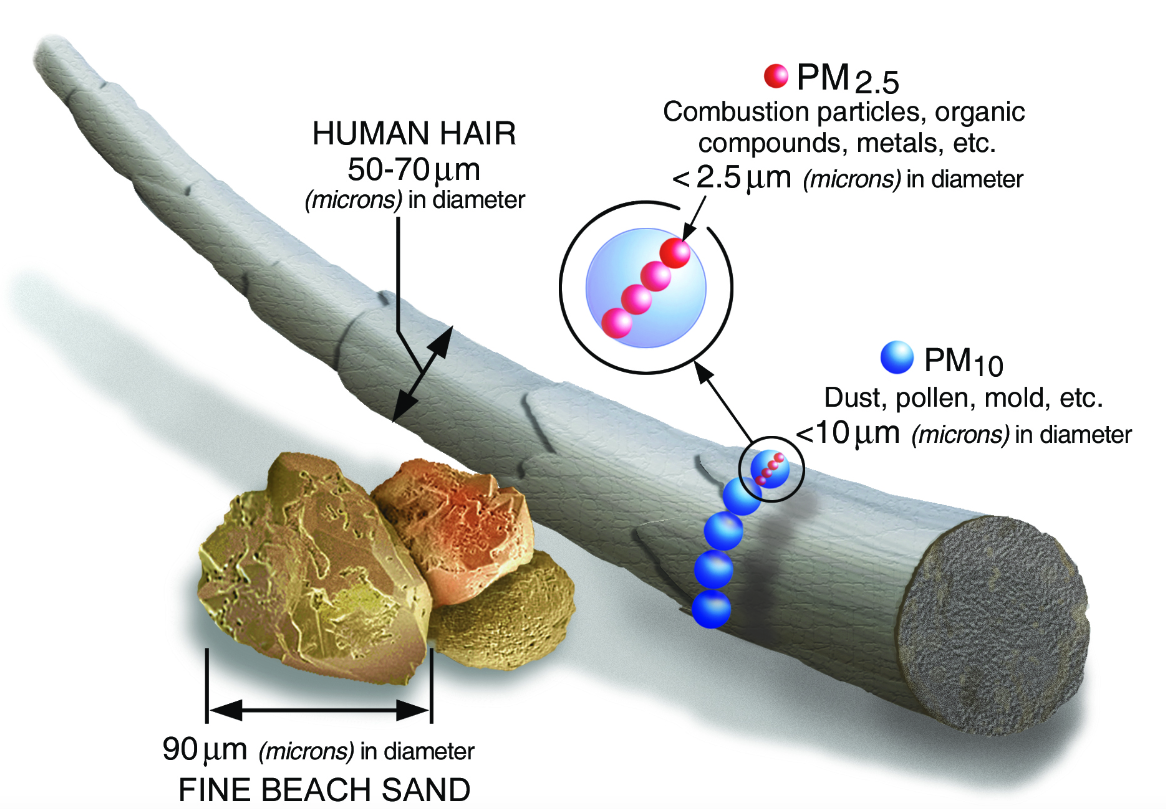
\includegraphics[width=0.75\columnwidth]{introduction/pm-size.png}
  \caption{Size comparisons for PM particles. Image source: US EPA
    (\url{https://www.epa.gov/pm-pollution/particulate-matter-pm-basics}, last
    accessed 2024-09-12).}
  \label{fig:pm-size-scale}
\end{figure}

PM is considered the most important air quality component due to its direct and
widespread impact on public health. Inhaled PM accumulates in the lungs, causing
both short-term and long-term health effects. Fine particulate matter,
specifically PM 2.5, is small enough to pass through the lungs and into the
bloodstream, increasing the risk of cardiovascular diseases, strokes, and cancer
\cite{pm-disease-1, pm-disease-2, pm-cancer}. Due to these combined effects, PM
exposure is estimated to be responsible for millions of premature deaths each
year \cite{pm-mortality-1, pm-mortality-fine}.

In response, many regulatory bodies have introduced new legislation explicitly aimed
at reducing PM levels. The European Union recently revised its air quality
standards to adopt a $10$ $\mu g/m^3$ annual limit for average PM 2.5.
The United States Environmental Protection Agency (EPA) has also adopted tighter
PM regulations, revising its annual PM 2.5 standard to $9$ $\mu g/m^3$ while
maintaining the $35$ $\mu g/m^3$ 24-hour limit.
These developments underscore the growing recognition of the threat posed by PM.


Annual and 24-hour PM regulations are designed to manage long-term exposure but
fail to capture acute spikes from short-term pollution events. These
transient PM spikes can lead to immediate increases in blood pressure, placing
vulnerable populations at heightened risk \cite{pm-bp}. Additionally, short-term
PM exposure has been shown to impair cognitive performance \cite{pm-cognition}.
In fact, the effects of PM on the body are strong enough that short-term PM 2.5
exposure can be independently estimated from a small assortment of biometric
sensors \cite{shawhin-biometrics, shisir-biometrics}. Therefore, high-resolution
PM data are essential for accurately quantifying the immediate impacts of local
PM pollution and facilitating timely mitigation efforts.

\section{Dissertation Goals}

The goal of this dissertation is to advance physical sensing in service of
society by leveraging physically motivated machine learning methods to extract
actionable insights from environmental data. Most modern machine learning models
are designed to solve \textit{general} learning tasks, such as image
classification and language prediction, for which the underly data may come
from a variety of sources with no representation in the real world.
In contrast to these abstract datasets, measurements from physical sensing systems
are governed by physical laws. This requirement imposes a strong constraint on
the space of possible model architectures; the predictions made
for environmental systems must be interpretable in their physical context. We
therefore adopt a physics-based approach, by which we mean machine learning
techniques which strike a balance between data-driven learning and domain-specific
knowledge. This approach includes
\begin{itemize}
\item \textbf{Physically motivated model selection}: The chosen model should
  align with the underlying physical principles of the system under study. For
  example, a model predicting particulate matter should be physically
  realizable so that negative concentrations are disallowed. Similarly, model
  assumptions for the underlying data distribution should apply to the
  measurement data.
\item \textbf{Integration of Prior Physical Knowledge}: Features corresponding
  to relevant physical quantities should be incorporated to improve model
  predictions. For example, the illumination geometry over a water body can
  significantly impact remote sensing imagery, and by extension, the
  estimation of water quality parameters.
\item \textbf{Interpretability}: Understanding \textit{how} a model makes
  predictions is just as important as prediction accuracy. Preference should be
  given to models with explainable structures. Additionally, the quantification of
  model uncertainty is vital for making informed decisions.
\end{itemize}
Towards this end, this work presents a collection of case studies utilizing both
supervised and unsupervised machine learning techniques for the assessment of
water quality and air quality.

In the first category, we are focused on answering the basic question:
\textit{Is this water safe?} Localized in situ measurements for specific water
quality parameters do not provide sufficient spatial coverage to assess water
quality across water bodies with variable topography, composition, and flow. Remote
sensing imagery can cover far wider areas, but simple empirical models
insufficient to robustly map complex spectra to contaminant concentrations. We
therefore utilize machine learning to bridge this gap.

For air quality measurement, our goal is to develop predictive models which can
resolve abrupt pollution spikes in PM time series while \textit{also} enabling
short-term forecasts. Many complicated machine learning models have been
developed for generic time series analysis. In this work, we focus on developing
physically-motivated models based on known PM dynamics. As secondary goal, these
models should be small enough to be deployable on low-cost sensing hardware.


\section{Research Contributions}

The research presented in this dissertation involved the collection of multiple
datasets \textit{and} the creation of software for data processing, modeling,
and analysis. The studies presented in Chapters~\ref{ch:robot-team-supervised}
and \ref{ch:robot-team-gtm} have been published in peer-reviewed journals. The
study from Chapter~\ref{ch:robot-team-gsm} is currently in review, and a
manuscript for the study presented in Chapter~\ref{ch:havok} is in preparation.
A comprehensive list of these various contributions is provided below in
Table~\ref{tab:contributions}


\begin{table}[H]
  \caption{Datasets, software, and publications developed for this dissertation.}
  \label{tab:contributions}
  \begin{center}
    \resizebox{\textwidth}{!}{\begin{tabular}{lccc} \hline
      \textbf{Title} & \textbf{Type} & \textbf{Chapter(s)} & \textbf{Status} \\ \hline
      Autonomous Learning of New Environments with a Robotic Team & & & \\
      Employing Hyper-Spectral Remote Sensing, Comprehensive In-Situ & Article & \ref{ch:robot-team} & published, \cite{robot-team-1}  \\
      Sensing and Machine Learning & & & \\ \hline
      Characterizing Water Composition With an Autonomous Robotic & & & \\
      Team Employing Comprehensive in Situ Sensing, Hyperspectral & Article & \ref{ch:robot-team-supervised} & published, \cite{robot-team-2} \\
      Imaging, Machine Learning, and Conformal Prediction & & & \\ \hline
      Unsupervised Characterization of Water Composition With & & & \\
      Uav-Based Hyperspectral Imaging and Generative Topographic & Article & \ref{ch:robot-team-gtm} & published, \cite{robot-team-gtm} \\
      Mapping & & & \\ \hline
      Generative Simplex Mapping: & & & \\
      Non-linear Endmember Extraction & Article & \ref{ch:robot-team-gsm} & Submitted, In Review \\
      and Spectral Unmixing for Hyperspectral Imagery & & & \\ \hline
      Interpretable Time-delay Embedding Models & & & \\
      for Low-Cost Particulate Matter Sensors: & Article & \ref{ch:havok} & In Preparation \\
      Forecasting and Outlier Detection & & & \\ \hline
      & & & \\
      \texttt{RobotTeam.jl} & Code & \ref{ch:robot-team}, \ref{ch:robot-team-supervised}, \ref{ch:robot-team-gtm}, \ref{ch:robot-team-gsm} & \href{https://github.com/john-waczak/RobotTeam.jl}{Julia Package} \\
      & & & \\ \hline
      & & & \\
      \texttt{SolarGeometry.jl} & Code & \ref{ch:robot-team-supervised} & \href{https://github.com/john-waczak/SolarGeometry.jl}{published, Julia Package} \\
      & & & \\ \hline
      & & & \\
      \texttt{GenerativeTopographicMapping.jl} & Code & \ref{ch:robot-team-gtm}, \ref{ch:robot-team-gsm} & \href{https://github.com/john-waczak/GenerativeTopographicMapping.jl}{published, Julia Package} \\
      & & & \\ \hline
      & & & \\
      \texttt{MLJNonnegativeMatrixFactorization.jl} & Code & \ref{ch:robot-team-gsm} & \href{https://github.com/john-waczak/MLJNonnegativeMatrixFactorization.jl}{published, Julia Package} \\
      & & & \\ \hline
      & & & \\
      HAVOK time series models & Code & \ref{ch:havok} & \href{https://github.com/john-waczak/aq-havok.jl}{Code repository} \\
      & & & \\ \hline

      & & & \\
      Live Air Quality Dashboards & (live) Data & \ref{ch:air-network} & \href{http://mdash.circ.utdallas.edu:3000}{Website} \\
      & & & \\ \hline
      & & & \\
      Air Quality Database & Dataset & \ref{ch:air-network},\ref{ch:havok} & \href{http://mdash.circ.utdallas.edu:8086}{Website} \\
      & & & \\ \hline
      & & & \\
      Robot team Hyperspectral Images & Dataset & \ref{ch:robot-team-supervised}, \ref{ch:robot-team-gtm}, \ref{ch:robot-team-gsm} & \href{https://ncsa.oxn.xsede.org/ees230012-bucket01}{OSN S3 Bucket} \\
      & & & \\ \hline
      & & & \\
      MINTS Air Network Historical Data  & Dataset & \ref{ch:air-network} & \href{https://ncsa.oxn.xsede.org/ees230012-bucket01}{OSN S3 Bucket} \\
      & & & \\ \hline
    \end{tabular}}
  \end{center}
\end{table}



\section{Dissertation Overview}

In Chapter~\ref{ch:robot-team} we first provide a general overview of the
interaction between light and water which motivates the use of hyperspectral imaging
for the assessment of water quality and composition. We then describe a
autonomous robotic team developed to coordinate drone-based hyperspectral imaging
with in situ data collection to greatly accelerate the data acquisition process
for water quality studies. We provide a detailed description of the
georeferencing and reflectance conversion procedures developed to process
hyperspectral images and conclude with an evaluation of total image processing times.

Next, in Chapter~\ref{ch:air-network} we outline measurement techniques for
particulate matter sensing before describing a low-cost network of distributed
air quality monitors designed to collect real-time PM data. We then describe a
containerized data pipeline combining multiple open-source tools to process
network data, provide live visualization dashboards, and enable redundant
data storage.

In Chapter~\ref{ch:robot-team-supervised} we develop a family of supervised
machine learning models to map reflectance spectra to key water composition
parameters. Importantly, this approach utilizes conformal prediction
to assess distribution-free confidence intervals for model predictions. We
examine the relative importance of model features to identify key wavelength
bins for each target variable. Each model is then applied to map the
distributions of physical, chemical, ionic, and biochemical parameters across a
North Texas Pond.

In Chapter~\ref{ch:robot-team-gtm} we expand the capabilities of the robot team
to address situations for which water contaminants are not known in advance. In
this scenario, ground-truth data are not available, and therefore, unsupervised
machine learning methods are needed to identify sources using only hyperspectral
images. We utilize Generative Topographic Mapping for this task and demonstrate
it's ability to visualize the spatial distribution of reflectance spectra across
the water. A rhodamine tracer die released into the pond is then used to
demonstrate that this unsupervised approach successfully identifies unique
spectral signatures which can be used to map contaminant dispersion.

Next, in Chapter~\ref{ch:robot-team-gsm} we present a novel, physics-based
method for unsupervised spectral unmixing and endmember extraction.
This approach builds on the latent variable structure of Generative Topographic
Mapping to directly model linear and nonlinear mixing of radiometric data.
The model is evaluated against Non-negative Matrix Factorization for a
synthetic dataset of mixed spectra from the USGS spectral database. We then
apply the method to unmix water-based hyperspectral images captured by the robot
team. The same rhodamine dye is used to test the ability of the method to map
the dispersion of unknown contaminants across the water.

In Chapter~\ref{ch:havok} we return to the air quality network in order to develop time
series models for local particulate matter data. Given that particulate matter
generally follows a diurnal cycle with intermittent pollution spikes, we
leverage the Hankel Alternative View of Koopman method to simultaneously model
PM time series \textit{and} extract these occasional spikes. We then utilize
this framework to develop short-term forecasting capabilities.

Finally, in Chapter~\ref{ch:future-work} we present directions for future work
before summarizing the conclusions for each study in
Chapter~\ref{ch:conclusions}.




% Big data in the physical sciences
% Comment on the annual data volumes produced by
% \begin{itemize}
%   \item LANDSAT
%   \item Sentinel
%   \item CERN
%   \item James Webb
%   \item SDO AIA
%   \item Medical Imaging (MRI, CT scans, etc...)
% \end{itemize}

% What is machine learning

% Use of machine learning in the physical sciences

% \begin{itemize}
%   \item Remote sensing (inter-instrument calibration, classification, object identification, change monitoring via the NDVI and similar indices, etc.)
%   \item Protein Folding
%   \item Drug discovery
%   \item Surrogate modeling (i.e. for PDE solvers - now very popular at NVIDIA)
% \end{itemize}


% \subsection{Supervised and Unsupervised ML}


% \subsection{Physics-based Machine Learning}





%\chapter{Physical Sensing for Environmental Quality Assessment}\label{ch:physical-sensing}

\chapter{A Coordinated Team of Autonomous Robots for the Rapid Assessment of
  Water Quality}\label{ch:robot-team}

As outlined in Chapter~\ref{ch:intro}, the accurate assessment of water
quality is essential for monitoring ecosystem health and ensuring the safety of
water resources. A plethora of physical parameters
influence local water quality such as turbidity, dissolved organic matter, chlorophyll
concentrations, and suspended particulate matter. Importantly, many of these
contribute measurably to the optical properties of water bodies via
their impact on the scattering and absorption of incident light. Hyperspectral
imaging, which enables the measurement of radiometric quantities
across hundreds of individual wavelength bins, offers a powerful tool for
assessing these parameters. By detecting the subtle variations in
reflectance across the ultraviolet (UV), visible, and Infrared (IR) wavelengths,
hyperspectral imaging enables the differentiation of various water constituents
in complex environments.

In this chapter, we first introduce relevant concepts from radiometry and their
relationship to the measurements made by hyperspectral imagers. We then
describe a variety of physical parameters relevant for the assessment of water
quality and their manifestations in radiometric data. Armed with this
information, we then describe the development of a robotic team incorporating both
drone-based hyperspectral imaging and autonomous in situ data collection with an
autonomous boat. Carefully orchestrating the collection of hyperspectral
images (HSI) coincident with reference data for water quality parameters of
interest allows us to collect data volumes in a few minutes comparable to
decades-long satellite campaigns.

The sensing framework described in this chapter has been published in
\cite{robot-team-1} and was utilized for the studies presented in
Chapters~\ref{ch:robot-team-supervised}, \ref{ch:robot-team-gtm}, and \ref{ch:robot-team-gsm}.


\section{Light and Water}\label{sec:imaging}

Perhaps the greatest achievement of 19th century physics was the unification of
electricity and magnetism by James Clerk Maxwell in which the phenomenon of
light propagation is fundamentally described by oscillations in the electric and
magnetic fields. Therefore, let us first consider a motivating example of
electromagnetic plane waves propagating in a dielectric medium before relating them to
the radiometric measurements made by physical sensors. Recall that Maxwell's
equations in matter are given by
\begin{equation}\label{eq:maxwell}
  \begin{aligned}
    \nabla \cdot \mathbf{D} &= \rho_f, & \nabla \times \mathbf{E} &= - \partial_t \mathbf{B}, \\
    \nabla \cdot \mathbf{B} &= 0, & \nabla \times \mathbf{H} &= \mathbf{J}_f + \partial_t\mathbf{D},
  \end{aligned}
\end{equation}
where $\rho_f$ is the free charge density and $\mathbf{J}_f$ is the free current
density. For linear media of permittivity $\epsilon$, and permeability $\mu$, we
have $\mathbf{D}=\epsilon\mathbf{E}$ and $\mathbf{H}=\frac{1}{\mu}\mathbf{B}$.
In a region where $\rho_f=0$ and $\mathbf{J}_f=0$, these equations reduce to the
wave equation for $\mathbf{E}$ and $\mathbf{B}$, admitting traveling plane-wave
solutions.

A monochromatic plane-wave traveling in the $\hat{x}$ direction is given by
\begin{equation}\label{eq:travelling-wave}
  \begin{aligned}
    \mathbf{E} &= \bar{E}_0\exp(i(\kappa x - \omega t))\hat{y}, \\
    \mathbf{B} &= \bar{B}_0\exp(i(\kappa x - \omega t))\hat{z},
  \end{aligned}
\end{equation}
where $\bar{E}_0$ and $\bar{B}_0$ are complex numbers
(absorbing the phase). Equation~\ref{eq:travelling-wave} trivially satisfies
$\nabla \cdot \mathbf{D} = 0$ and $\nabla \cdot \mathbf{B} = 0$. Substitution into
the remaining equations yields the familiar dispersion relation for
electromagnetic waves:
\begin{equation}
  \kappa^2 = \omega^2\mu\epsilon
\end{equation}

Allowing for $\sqrt{\mu\epsilon}$ to be complex, we can decompose $\kappa$ into
\begin{equation}
  \kappa = \frac{2\pi m}{\lambda}
\end{equation}
where $m=n - ik$ is the \textit{complex index of refraction}. Substituting this expression
into Equation~\ref{eq:travelling-wave} and taking the real part, we obtain
\begin{equation}\label{eq:wave-real}
  \begin{aligned}
    \mathbf{E} &= E_0\exp\left(-\frac{2\pi k x}{\lambda}\right)\cos\left(  \frac{2\pi n x}{\lambda} - \omega t  + \phi \right) \hat{y} \\
    \mathbf{B} &= B_0\exp\left(-\frac{2\pi k x}{\lambda}\right)\cos\left(  \frac{2\pi n x}{\lambda} - \omega t  + \phi \right) \hat{z} \\
  \end{aligned}
\end{equation}

Instruments like the hyperspectral imagers do not measure
the time-dependent amplitudes of the electric and magnetic fields. Instead, they
detect energy deposited through a surface carried by these fields. This energy
flow is characterized by the Poynting vector, $\mathbf{S} =
\frac{1}{\mu}\mathbf{E}\times\mathbf{B}$ which has units of $W/m^2$, in other
words, the energy flux through a surface. Additionally, the sample rates of realistic
instruments are much longer than oscillations in $\mathbf{E}$ and $\mathbf{B}$ so
that the time-averaged Poynting vector $\langle
\mathbf{S} \rangle$ is really measured. Given that $\langle  \cos^2(\theta) \rangle =
1/2$, this results in
\begin{equation}
  \langle \mathbf{S} \rangle = \frac{1}{2}\sqrt{\frac{\epsilon}{\mu}}E_0^2\exp\left(-\frac{4\pi k x}{\lambda}\right) \hat{x}
\end{equation}

Here we see an important consequence of considering a complex index of reaction:
the quantity $a(\lambda)=4\pi k/\lambda$ is called the \textit{absorption coefficient}
which characterizes the amount of incident radiation absorbed by the medium as a
function of the penetration distance $x$. In low-turbidity coral reefs this helps
explains why red colors become muted at increasing depths. Finally, we note that
for a homogeneous solution containing $n$ chemicals, the Bouguer-Beer-Lambert law
relates the total absorption coefficient to each chemical concentration via
\begin{equation}
  a(\lambda) = \sum_i^n c_i\varepsilon_i(\lambda)
\end{equation}
where $c_i$ is the concentration of the $i$-th chemical species in the solution,
and $\varepsilon_i(\lambda)$ is the wavelength-dependent molar absorption
coefficient. The connection between the concentration of constituents in the
water to the interaction of a mixture with incident light motivates the
assessment of water quality by spectroscopic techniques.

\subsection{Radiometry}

\textit{Radiometry} is the science of the measurement of electromagnetic energy
and involves a number of derived quantities. As outlined in the previous
section, most optical and spectroscopic instruments do not directly measure the
oscillations in the electric and magnetic fields, but rather the energy they
transport into a sensing element. 

The \textit{spectral radiance} is defined as
\begin{equation}
  L(\mathbf{x}, t, \hat{\xi}, \lambda) = \frac{\partial^4 Q}{\partial t \partial A \partial \Omega \partial \lambda},
\end{equation}
or in words, the amount of incident radiant energy per area per
second, per solid angle, per wavelength. Importantly, the spectral radiance
depends on the sampling position $\mathbf{x}$ and time $t$ as well as the wavelength
$\lambda$ and direction of light $\hat{\xi}$. Historically many different
conventions for naming radiometric quantities have been used. We follow the
conventions used in \cite{mobley-text} for which the prefix \textit{spectral} is
used to indicate the explicit \textit{per-wavelength} dependence of a
radiometric quantity. $L$ is the fundamental measured quantity which captures
the spatial, temporal, spectral, and orientation dependencies of the light field.

When an instrument samples light from \textit{all} possible directions passing
through a collection area, then the
measured quantity is the \textit{spectral radiance}. Naturally, this quantitiy
depends on the orientation of the sensor. For example, the \textit{downwelling
  spectral radiance}, $E_d$ is defined by
\begin{equation}
  E_d(\mathbf{x}, t, \lambda) = \int_0^{2\pi} \int_0^{\pi/2}L(\mathbf{x}, t, \theta, \phi, \lambda)\cos\theta \sin\theta d\theta d\phi
\end{equation}
where the factor of $\cos\theta$ accounts for the apparent area at an angle
$\theta$ from the surface normal.

Different materials lead to different distributions of scattered light. For
\textit{specular} materials such as polished mirrors or the air-water interface, light
reflected at the surface leaves at an angle identical to the angle of incidence.
The polar opposite of a specular material is a \textit{Lambertian}, or perfectly
diffuse material. Light scattering off of a Lambertian surface is distributed
equally in all directions so that $L$ is independent of $\theta$ and $\phi$. As
a consequence, the spectral irradiance of light from a Lambertian surface is
\begin{equation}
  E = \int_0^{2\pi}\int_0^{\pi/2} L(\mathbf{x}, \lambda)\cos\theta \sin\theta d\theta d\phi = \pi L
\end{equation}

Given measurements for the downwelling (incident) and upwelling spectral
irradiances, the \textit{reflectance} is defined by their ratio:
\begin{equation}
  \rho(\mathbf{x},\lambda) = \dfrac{E_u(\mathbf{x}\lambda)}{E_d(\mathbf{x}, \lambda)}.
\end{equation}
This quantity is valuable as it extracts the useful signal from an image by
\textit{dividing out} the spectrum from the lighting source, in this case,
incident solar radiation.

\subsection{Optical Properties of Water Bodies}\label{sec:optical-properties-water}

The formulation of Maxwell's equations in Equation~\ref{eq:maxwell} treats
macroscopic media as continuous. However, at atomic scales, bodies of water
consist of collections of molecules (\ce{H2O} and other dissolved substances)
together with particulates which vary in size. The interaction of light with
these particles can be approximated by the interaction of light with dielectric
spheres with a specific radius and (potentially complex) index of refraction.
The general solution for the scattered intensity field of light by a dielectric
sphere of \textit{any} radius is known as \textit{Mie Theory} and involves
highly complicated expressions of infinite series of spherical multi-pole
expansions which can be evaluated numerically.

A special case for elastic scattering by particles with a diameter $d <<
\lambda$ is known as \textit{Rayleigh Scattering}. In this regime, the scattered
intensity obeys
\begin{equation}
  I = I_0  \left( \frac{2\pi}{\lambda} \right)^4 \left( \frac{d}{2} \right)^6 \left( \frac{1 + \cos^2\theta}{2R^2} \right)
\end{equation}
where $\theta$ is the scattering angle, $R$ is the distance from the particle to
the measurement point, and $n$ is the (real) index of refraction. Lord Rayleigh
used the $\lambda^{-4}$ dependence of this expression to explain why the sky is
blue: atmospheric particles (which we now understand to be gas molecules) with
diameters much smaller than visible wavelengths scatter blue light
much more than red light.

In addition to scattering, molecules and particulates can absorb incident light
according to their specific structure. For pure water, electronic transitions
lead to absorption in the UV while rotational and vibrational modes are relevant
at longer wavelengths. Critically, there is a transparent \textit{window} of low
absorption for visible wavelengths which enables aquatic life to access solar
energy.

Water bodies contain a variety of constituents leading to a continuous size
distribution from chemicals at the atomic scale ($\sim$$0.1$ nm) to virus
($\sim$$100$ nm), to aquatic animals ($\sim$$1$ m). These components are traditionally
classified into dissolved or particulate matter of organic or inorganic origin.
Most water bodies contain a variety of dissolved salts. For ocean waters these
account for roughly 3.5\% by weight while fresh water bodies tend to contain
trace amounts. Natural waters also contain a variety of dissolved organic
compounds produced by the decay of plant matter. These compounds mostly include
fulvic and humic acids which impart a yellowish-brown color in sufficient
conecntrations and are referred to in the literature as \textit{colored
  dissolved organic matter} (CDOM) \cite{cdom-acids}. Inorganic particulate
matter in natural waters is largely due to the weathering of rocks in soils
while organic particulates include bacteria, phytoplankton, zooplankton, and
larger organic detritus.

Light absorption by CDOM can be reasonably modeld using an exonential function
of the form
\begin{equation}
  a(\lambda) = a(\lambda_0)\exp(-S_g(\lambda - \lambda_0))
\end{equation}
for a reference wavelength $\lambda_0$ \cite{aurin2018remote}. The exact
value of the spectral slope $S_g$ depends on the proprotions of specific types
of CDOM with typical values on the order of $\sim$$0.01$.

Absorption by phytoplankton and many other organic sources is largely due to
photosynthetic pigments with cells such as chlorophyll. Chlorophyll a
absorption is strongest for blue and red wavelengths with peaks at
$\lambda\approx 430$ nm and $\lambda\approx 665$ nm, respectively. Other
relevant pigments include phycoerythrin and phycocyanin  which occur in
blue-green algae. Estimations of their concentration from remote sensing imagery
has been used to track the evolution of harmful algal blooms which often occur
due to increased nutrient concentrations from agricultural and urban runoff
\cite{algal-blooms-rs}.

Lastly, we note that in addition to scattering and absorption, many chemicals
such as crude oil and organic components such as CDOM and chlorophyll undergo
fluorescence when excited at appropriate wavelengths. For example, CDOM excited
by UV light with $\lambda\in[250, 400]$ nm will emit at wavelengths in
$\lambda\in[400, 500]$ depending on the specific types of organic compounds
\cite{cdom-fluorescence}. Fluorometers calibrated for these excitation
and emission properties can therefore be used for in situ assessment of many
water constituent concentrations.

\section{Coordinated Robot Teams}

For decades, multi-spectral imagers which sample a small number of
broad wavelength bands have seen widespread use in
the remote sensing community as a means to take advantage of the wealth of
information contained in the reflectance spectra of materials. Multi-spectral imagers,
like those deployed on MODIS, Sentinel 2, and other satellite platforms, include
wavelength bands ranging from the near-UV,
through the visible spectrum, and into the Infrared and have been applied in a
variety of domains from tracking land change, characterizing deforestation,
monitoring erosion, evaluating crop health, and many others
\cite{remote-sensing-foliage, remote-sensing-applications, thenkabail-indices}.

\begin{figure}[!hbt]
  \centering
  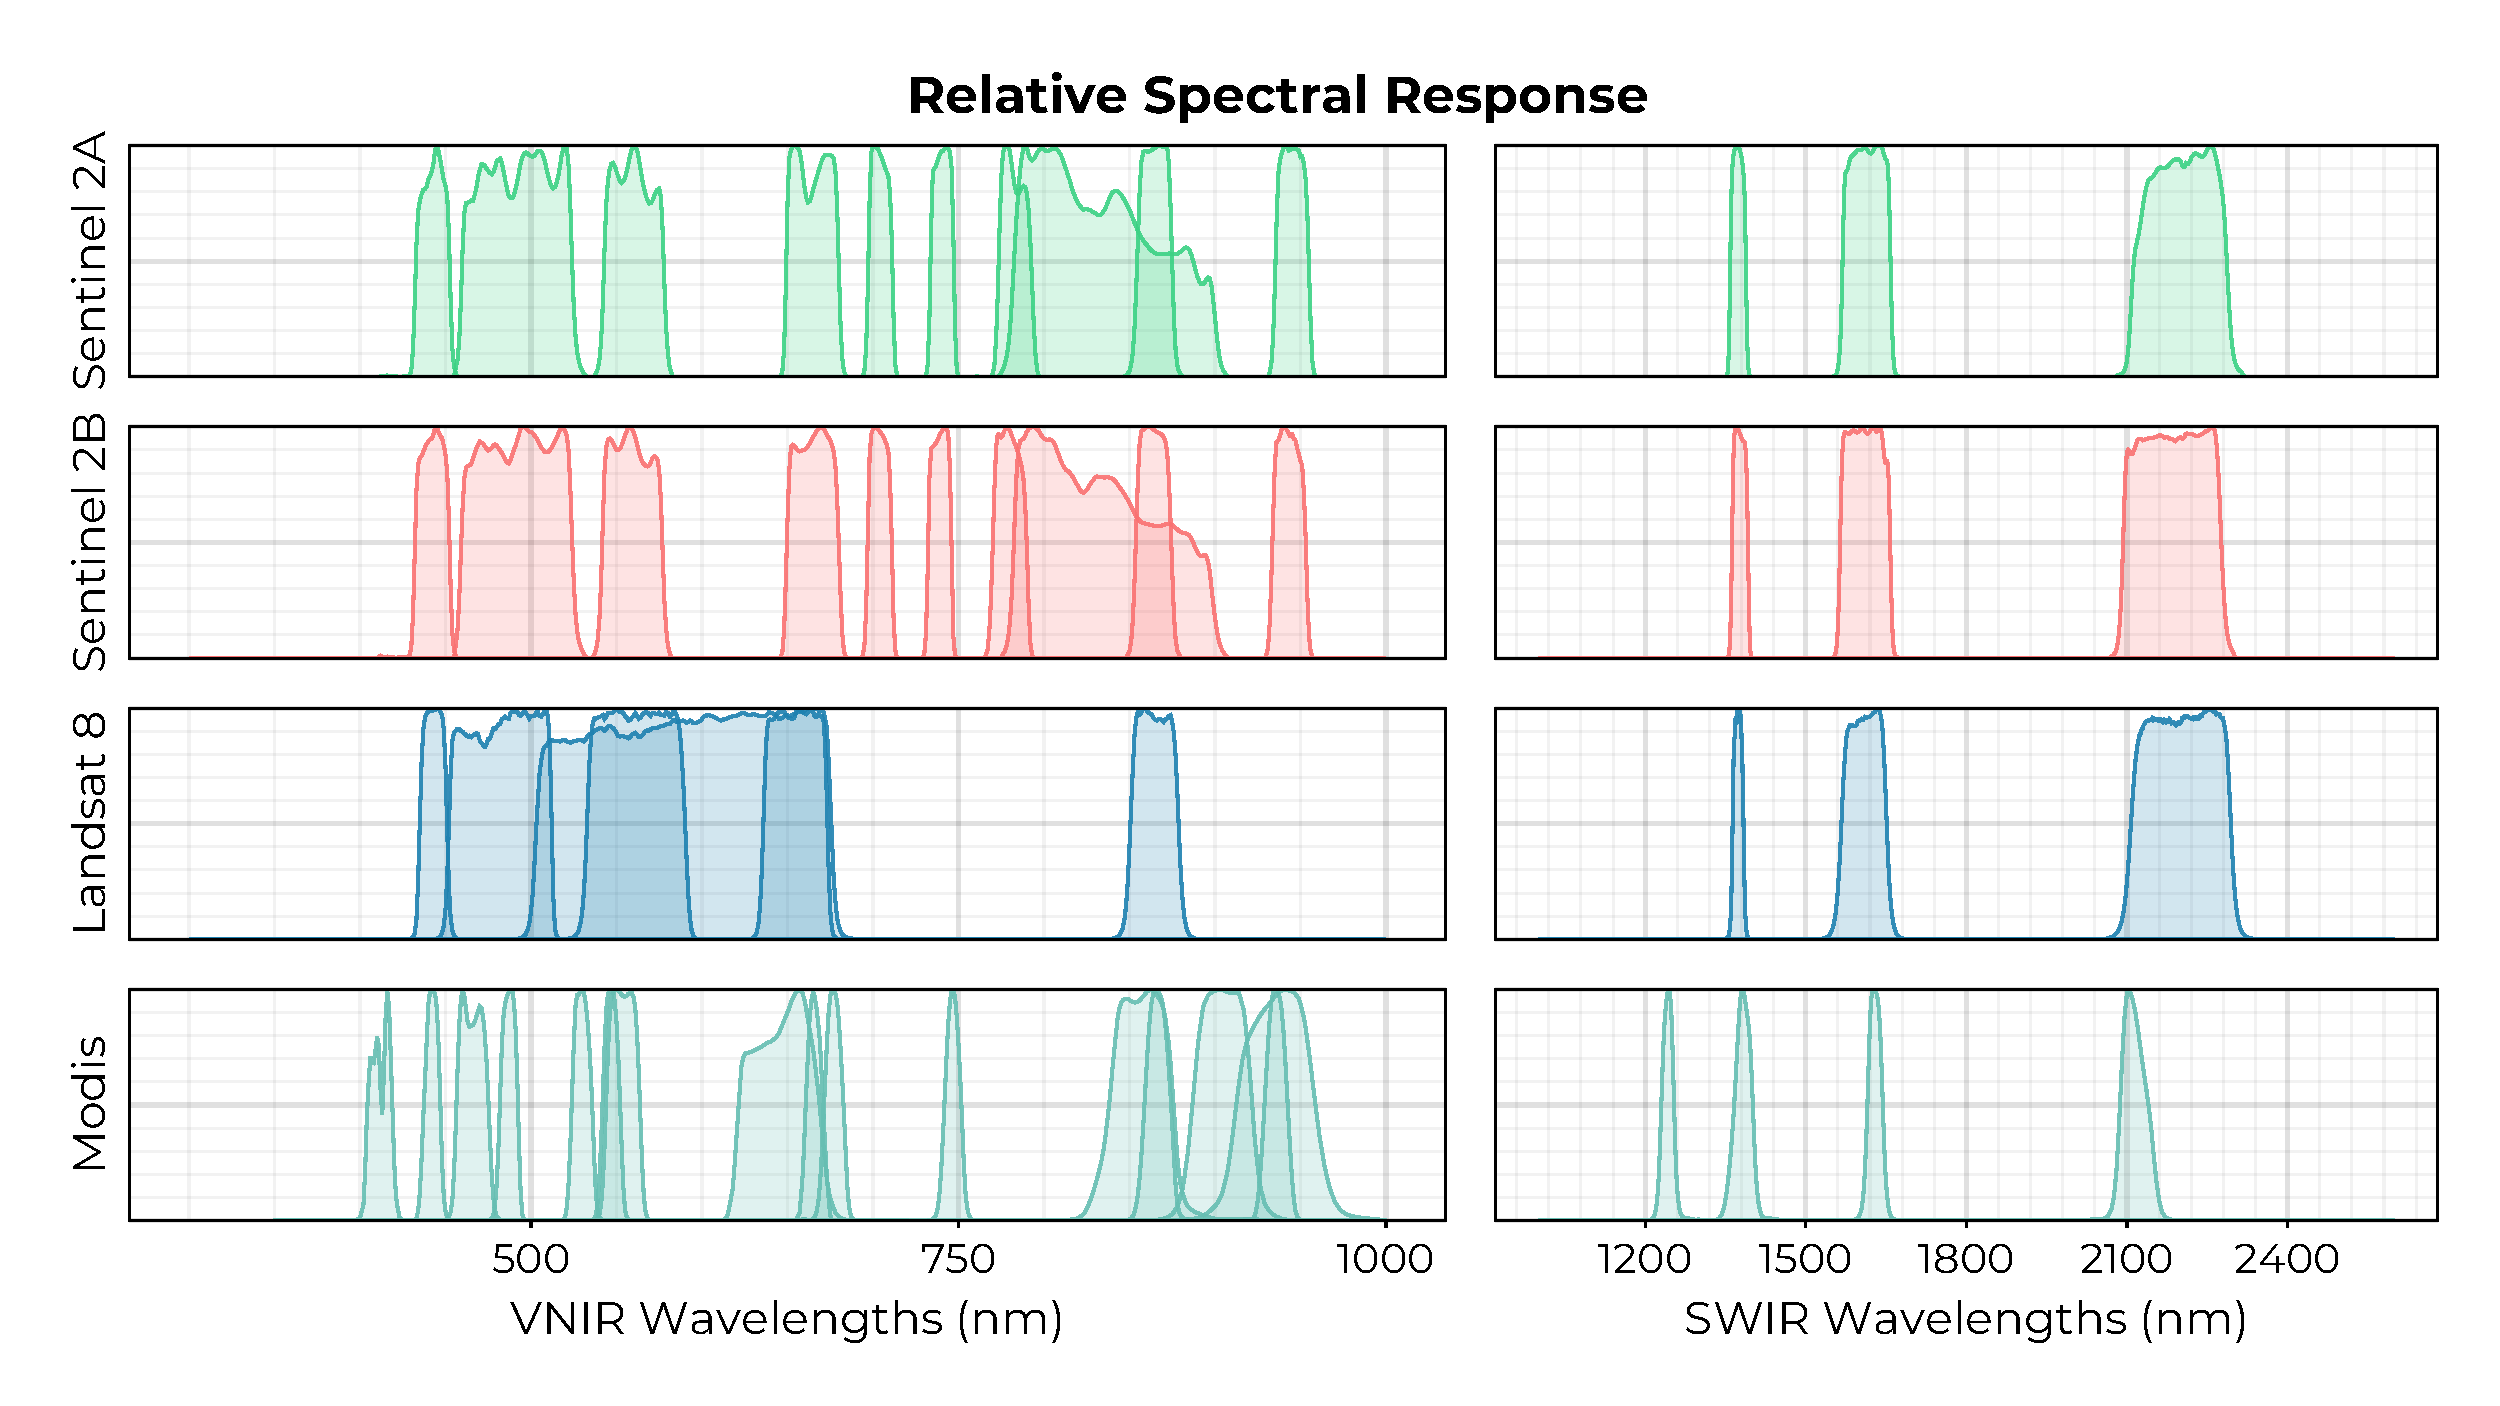
\includegraphics[width=0.85\columnwidth]{robot-team/passbands.pdf}
  \caption{A comparison of the relative spectral response for the passbands of popular multi-spectral imaging remote sensing platforms.}
  \label{fig:passbands}
\end{figure}

Many currently used spectral indices like the normalized difference vegetation
index (NDVI) take advantage of spectral features by comparing ratios of
pigment sensitive passbands to the stable signals in the infrared to infer the
abundance of chlorophyll, and consequently, the health of plants
\cite{ndvi-chlorophyll}.  However, despite the many successful
applications of multi-spectral imaging, there are a few key limitations which
impact their use for the assessment of water quality.

\begin{enumerate}
  \item Multi-spectral imagers have limited use for the assessment of many
    constituents affecting water quality whose spectral features overlap in the
    broad wavelength bands of systems like those shown in Figure~\ref{fig:passbands}.
  \item Satellite-based instruments measure top of atmosphere reflectance and
    must be carefully corrected to obtain values at the surface by accounting for
    absorption and scattering by atmospheric gases and particulates.
  \item Validating models which map remotely sensed reflectance to parameters of
    interest requires the collection of in situ reference data. This relies on
    serendipetous satellite passes over sensing sites often requiring decades of
    observations to collect sufficient quantities needed for model training and
    validation \cite{aurin2018remote, ross2019aquasat}.
\end{enumerate}

Hyperspectral imagers are designed to measure spectral radiance for many
hundreds of wavelengths at each image pixel. Their improved spectral resolution
makes it possible to detect fine spectral features. Developments in
hyperspectral imaging technology have led to dramatic reductions in both their
size and weight so that it is now possible to incorporate the
technology as the payload of highly mobile unmanned aerial vehicles (UAV) such as
drones. By collecting hyperspectral images (HSI) close to the ground, we limit
the need for complicated atmospheric corrections while enabling centimeter-scale
spatial resolutions. However, the massive size of HSI poses a significant
computational challenges for their adoption in real-time
applications.

The typical timescale from starting work on a new remote sensing data
product to its operational readiness is at least a couple of years, but, more
typically, a decade or more. Our goal is to reduce this timescale to be near
real time by utilizing an autonomous robotic team that can both collect the
training data, and then in real time process and stream the remote sensing data
products. The fully autonomous team includes an uncrewed surface vessel (USV)
that carries a suite of sensors to measure in situ water composition,
and an autonomous UAV equipped with a hyperspectral imager, downwelling
irradiance spectrometer, thermal imagers, and embedded compute for onboard machine
learning capabilities. Figure \ref{fig:drone-team} shows photographs of the robot team
during a deployment in North Texas.

\begin{figure}[!hbt]
  \centering
  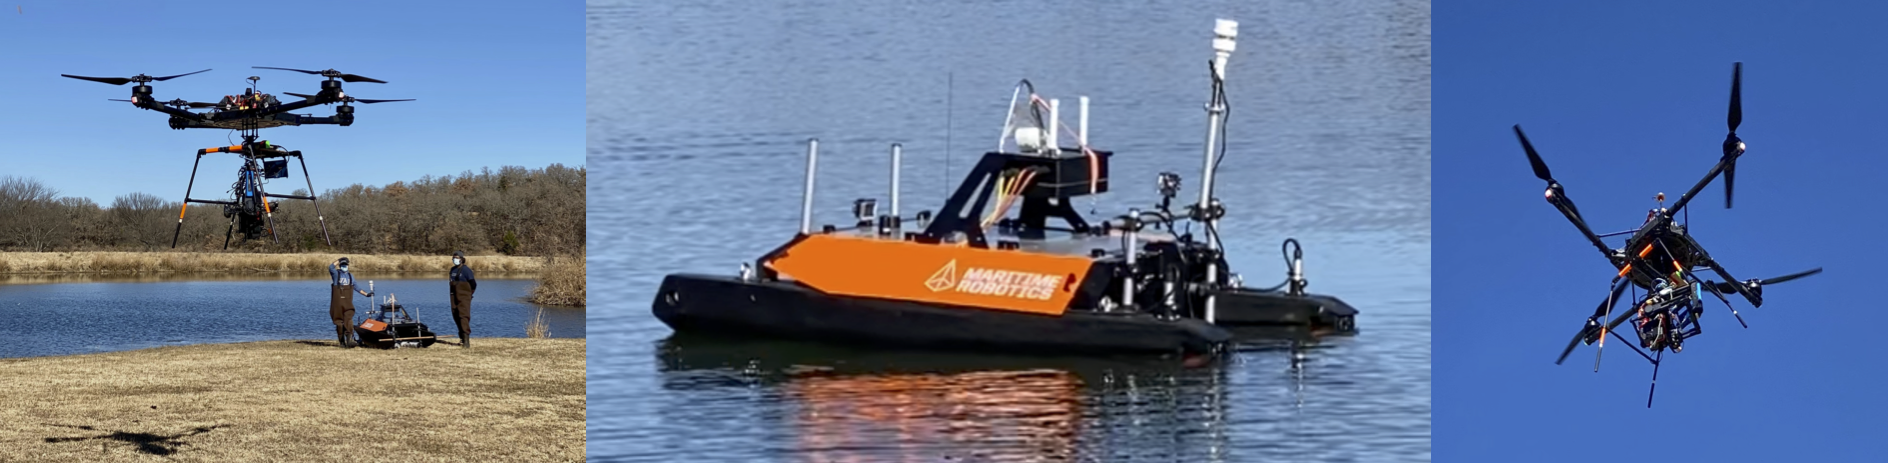
\includegraphics[width=0.9\columnwidth]{robot-team/robot-team-photos.png}
  \caption{The autonomous robotic team. (\textbf{left}) The drone hovering a few
  feet above the ground during take-off. (\textbf{center}) the USV deployed in
  the water. (\textbf{right}) The drone as seen from below.}
  \label{fig:drone-team}
\end{figure}

The autonomous boat used is a
\href{https://www.maritimerobotics.com/otter}{Maritime Robotics Otter }. With a
footprint of only 200 × 108 × 81.5 cm, a weight of 55 kg, and dual electrical
fixed thrusters, it is an easily deployable asset that can be transported in a
van or even within normal airliners to a survey site. At a cruise speed of two
knots, it has a duration of approximately 20 hours per battery charge. It can use
WiFi, cellular, and an optional AIS receiver for communication to the control
station. Our drone is a \href{https://freeflysystems.com/alta-x}{Freefly Alta-X}
professional quad-copter. It was specifically designed to carry cameras, with a
payload capacity of up to 35 lb, a long range data link, and autonomy provided
by the Open PX4 flight stack. The open source QGroundControl software is used to
control the autonomous operations.

Both the UAV and USV carry high-accuracy GPS and inertial
measurement units (IMU) so that every data point can be georeferenced and time
stamped. Each robot can also join the same wireless network which connects the
robots and a ground control stations. For the deployments described in
Chatpers~\ref{ch:robot-team-supervised}, \ref{ch:robot-team-gtm}, and
\ref{ch:robot-team-gsm}, long-range
\href{https://www.ui.com}{Ubiquiti 5 GHz LiteBeam airMAX WiFi} was used for
data transfer and control. The network
also includes a local \href{https://www.synology.com}{Synology network-attached
  storage (NAS)} device which syncs collected data to another NAS in our home laboratory at the
UT Dallas for redundancy.

The robotic boat payload includes a
\href{https://www.biosonicsinc.com/products/mx-aquatic-habitat-echosounder/}{BioSonics
  MX Aquatic Habitat Echosounder sonar} for rapid assessment and mapping of
aquatic vegetation, substrate and bathymetry. Three
\href{https://www.waterprobes.com/multiprobes-and-sondes-for-monitori}{Eureka
  Manta-40 multi-probes}, a
\href{https://www.sequoiasci.com/product/lisst-abs/}{Sequoia Scientific
  LISST-ABS acoustic backscatter sediment sensor}, and an
\href{https://www.airmar.com/weather-description.html?id=153}{Airmar Technology
  Corporation 220 WX ultra-sonic weather monitoring sensor}.

The first Manta-40 multi-probe includes sensors for temperature and turbidity
and
\href{https://www.turnerdesigns.com/cyclops-7f-submersible-fluorometer}{Turner
  Designs Cyclops-7 submersible Titanium body fluorometers} for chlorophyll a,
chlorophyll a with red excitation, blue-green Algae for fresh water
(phycocyanin), blue-green Algae for salt water (phycoerythrin), and CDOM.
The second Manta-40 multi-probe includes sensors for temperature, conductivity
(with specific conductance, salinity, and total dissolved solids, TDS), pH (with
separate ref-erence electrode), optical dissolved-oxygen, turbidity, and ion
selective electrodes by Analytical Sensors and Instruments
(\url{http://www.asi-sensors.com/}, accessed 05/01/2021) for ammonium
(\ce{NH4^+}), bromide (\ce{Br^-}), calcium (\ce{Ca^2+}), chloride (\ce{Cl^-}),
nitrate (\ce{NO3^-}), and sodium (\ce{Na^+}). The third Manta-40 multi-probe
includes sensors for temperature, turbidity, a total dissolved gas sensor, and
additional fluorometers for measuring optical brighteners, crude oil, refined
fuels, and tryptophan.

\begin{figure}[!hbt]
  \centering
  \includegraphics[width=0.9\columnwidth]{robot-team/annotated-drone.pdf}
  \caption{An annotated view of the autonomous drone showcasing the hyperspectral imager and onboard compute.}
  \label{fig:uav-closeup}
\end{figure}

Custom landing gear gear made from light-weight
carbon fiber was manufactured for the UAV to maximize the potential carry
capacity. The installed hyperspectral imager is a
\href{https://resonon.com/Pika-XC2}{Resonon Visible+Near-Infrared (VNIR) Pika
  XC2}, and thermal images are captured with
a \href{https://www.flir.com/products/duo-pro-r/}{FLIR Duo Pro R} installed
in a parallel configuration as indicated in Figure~\ref{fig:uav-closeup}. On top
of the UAV, a sky facing Ocean Optics UV-Vis-NIR spectrometer with an included
cosine corrector measures the incident downwelling irradiance to enable the
conversion of radiance hyperspectral data cubes to reflectance.

During a single 30 minute deployment, the robot team is able to autonomously
collect over a terabyte of HSIs together with over 10,000 in situ measurements
from the suite of sensors on the USV. Coordinating UAV flights to overlap USV
data collection makes it easy to identify reflectance spectra collocated with
USV measurements. This in turn makes it possible quickly train machine learning
models mapping HSI reflectance spectra to water quality parameters of interest.
Once trained, the models may be deployed directly onto the UAV computer to allow
streaming of concentration maps to the ground station during subsequent flights.
The machine learning models developed for the robot team are described in
Chapter~\ref{ch:robot-team-supervised}. Additionally, unsupervised techniques
for assessing the presence of unanticipated contaminants are developed in
Chapters~\ref{ch:robot-team-gtm} and
\ref{ch:robot-team-gsm}.

In the final sections of this chapter, we present the methods implemented to
rapidly georectify captured HSI and convert their radiance measurements to
reflectance using secondary spectra from the downwelling irradiance
spectrometer. This process quickly assigns latitude and longitude coordinates to
each HSI pixel making it possible to generate maps of the reflectance
distribution across an entire body of water. The coordiantes of georectified HSI
are also used to collocate reflectance spectra with in situ USV measurements.



\section{Rapid Processing and Georectification of Hyperspectral Data Cubes}

For an HSI platform to operate in (near) real-time, three key tasks are critical:
\begin{enumerate}
\item \textbf{FileIO}: Raw HSI need to be quickly read by the on-board processing computer.
\item \textbf{Georectification}: HSI must be georeferenced so that each image
  pixel can assigned a location on the ground.
\item \textbf{Radiometric Conversion}: HSI data cubes need to converted to the
  desired radiometric quantity, i.e. the reflectance.
\end{enumerate}

The first item is readily accomplished by means of light-weight, high-volume
solid state drives incorporated into the UAV computer. To address the second, we
need both sufficient compute capabilities and optimized processing software. The
final item relies on both the georectified data cube and the secondary
irradiance spectrum captured by the upward facing downwelling irradiance
spectrometer. To enable this workflow, the UAV utilizes a pair of light-weight
processing computers (Intel NUCs) each have 12 cores and 64 gigabytes of
installed RAM.  One is attached directly to the imager and
manages data acquisition by the camera and saving of raw HSI files. The second
NUC is mounted above the payload and serves as the onboard data processing unit. These
computers can be seen in panels (a) and (b) of Figure~\ref{fig:uav-closeup}.

%The upward facing spectrometer captures the \textit{downwelling} irradiance
%spectrum, $E_d(\lambda)$ which is necessary to enable conversion from radiance units to the

The georectification procedure implements for HSI from the UAV is based on the
methods described in \cite{muller2002program, baumker2001new, mostafa2000multi}
for pushbroom-mode hyperspectral imagers while the reflectance conversion
assumes Lambertian scattering as described previously in Section~\ref{sec:imaging}.
The processing steps are as follows:

\begin{enumerate}
\item Raw imagery (radiance spectra) are continuously captured by the hyperspectral imager and stored in binary ENVI format.
\item The processing computer read an ENVI file into a multi-dimensional array
  once it finishes writing.
\item Associated flight data (GPS and IMU) are read.
\item Flight data are interpolated to match the sample times for each HSI scan-line.
\item Each scan-line is georeferenced to obtain coordinates (lat,lon) for each pixel.
\item The georeferenced HSI is then resampled to a regular grid spatial grid.
\item The downwelling irradiance spectrum associated with the HSI is read.
\item The downwelling spectrum is interpolated to match the wavelength bins of the HSI
\item The HSI is converted o reflectance.
\item Spectral indices (NDVI, etc...) are computed.
\item The final data cube is saved to an HDF5 file.
\end{enumerate}
A visual representation of the pipeline is shown in
Figure~\ref{fig:hsi-pipeline} below.
\begin{figure}[H]
  \centering
  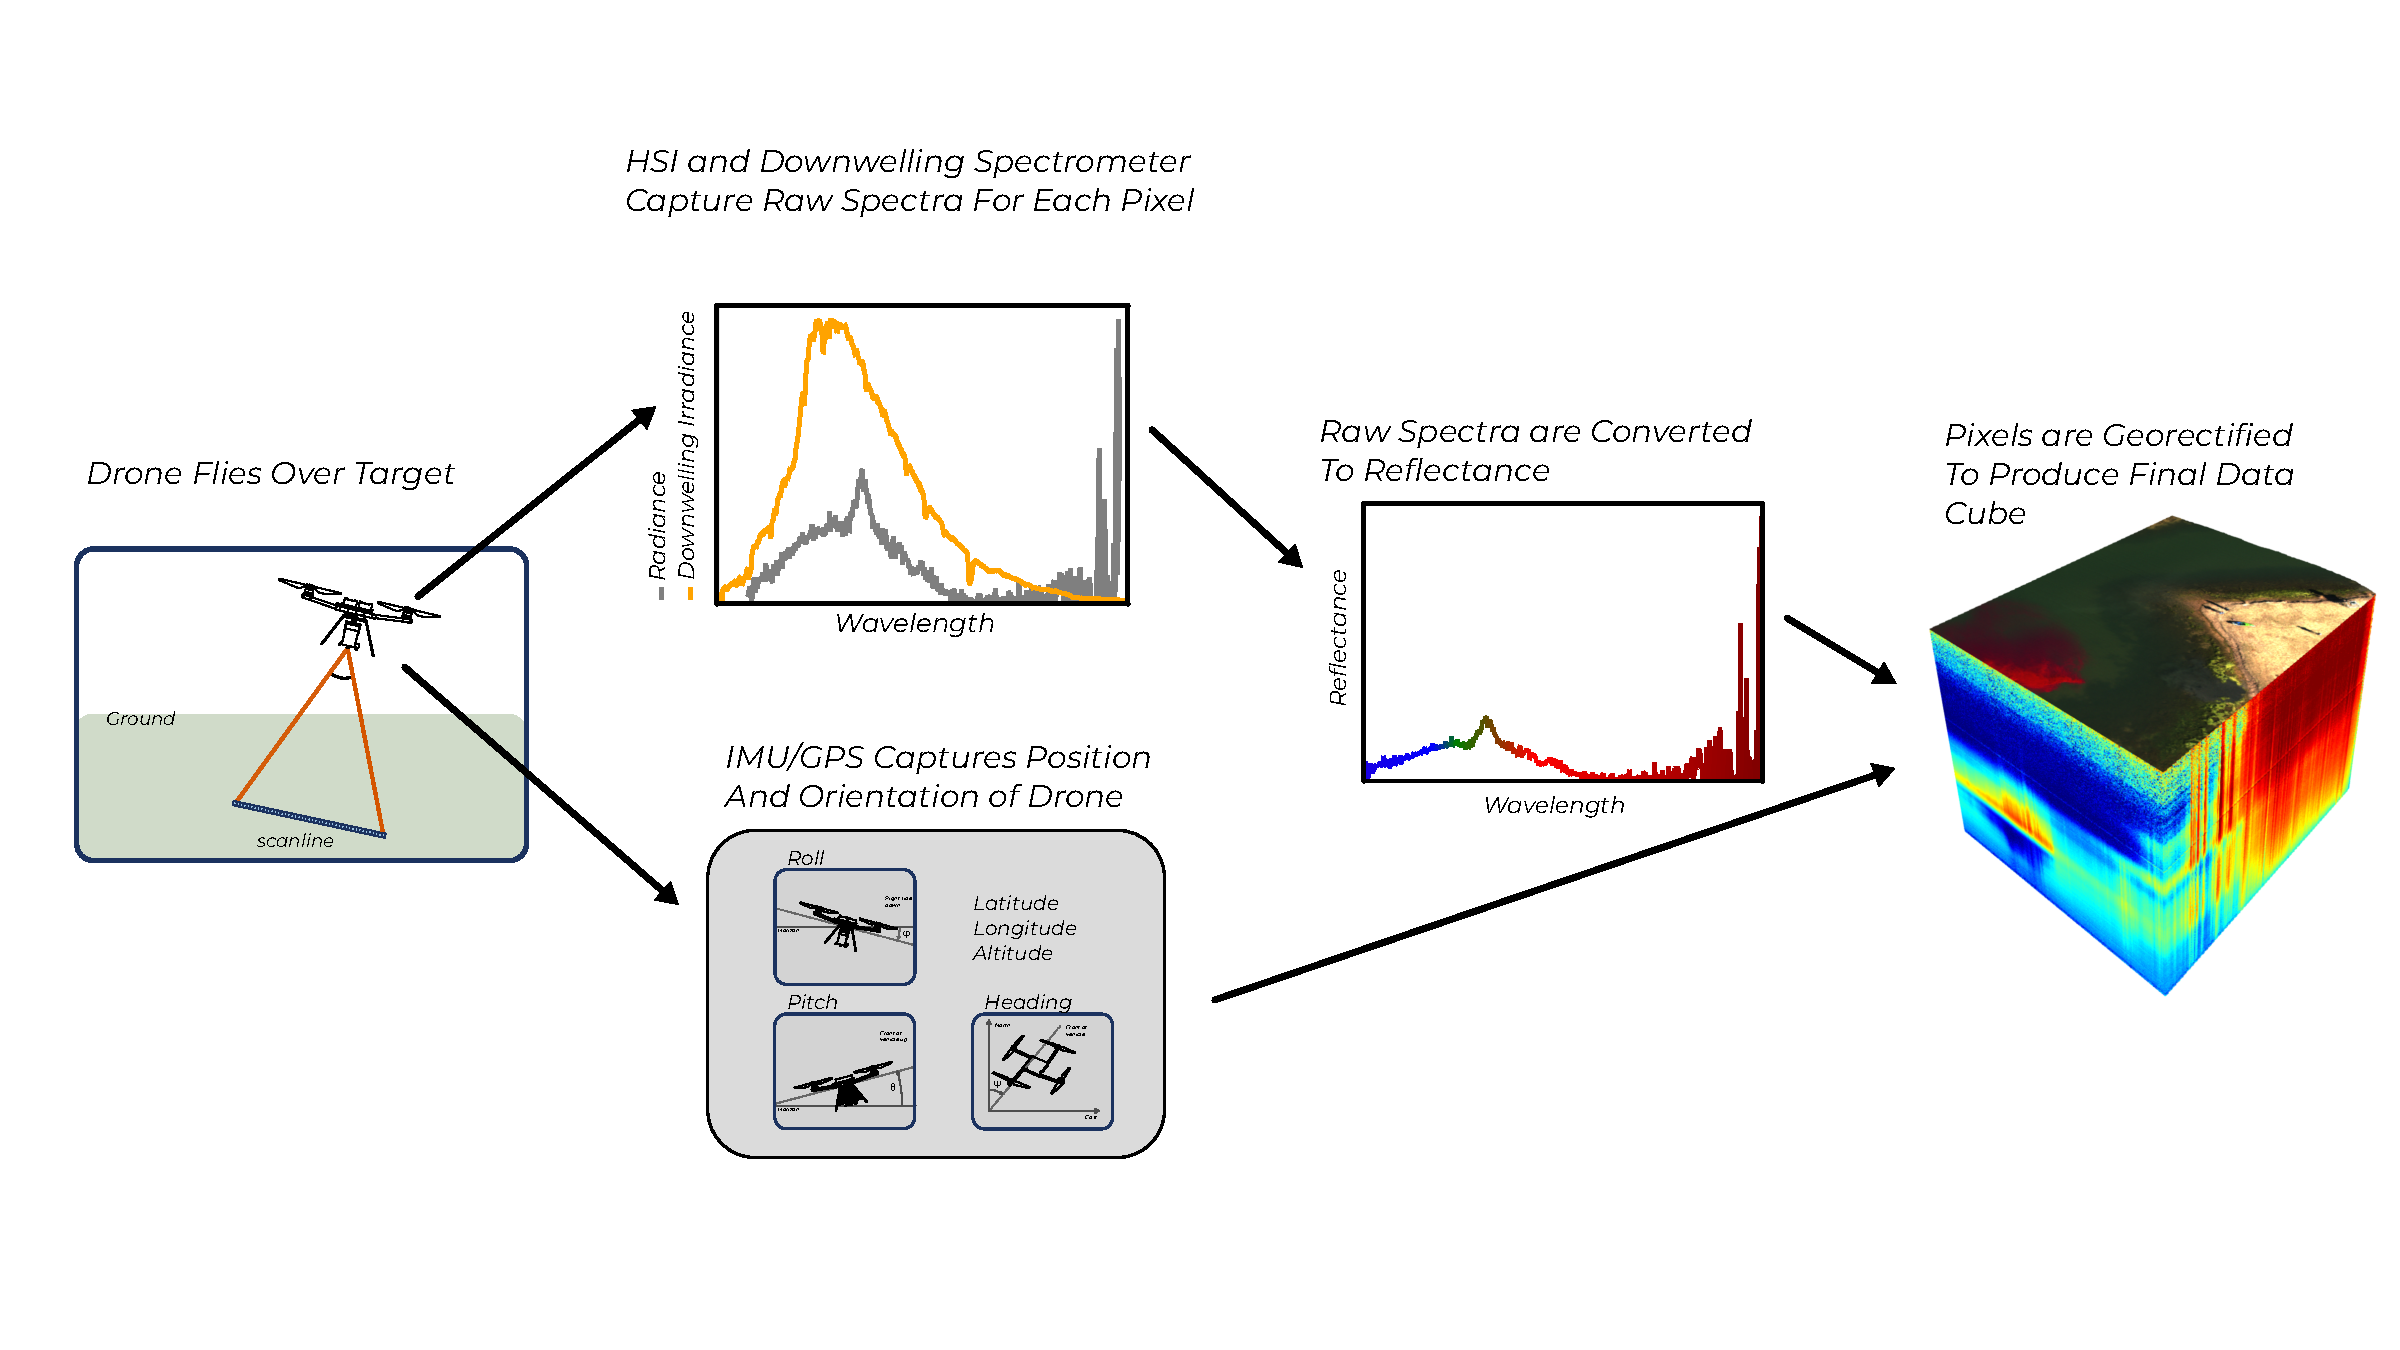
\includegraphics[width=\columnwidth]{robot-team-supervised/materials-and-methods/pipeline-figure-2.pdf}
  \caption{Hyperspectral image processing: Hyperspectral data cubes are
    collected one scan-line at a time (left). By utilizing downwelling
    irradiance spectra, we convert each pixel from spectral radiance to
    reflectance. By using orientation and position data from the on-board GPS
    and INS, we georeference each pixel to assign it a latitude and longitude on
    the ground. The final data product is the georectified hyperspectral
    reflectance data cube (right) visualized as a pseudo-color image with
    reflectance  as a function of wavelength along the
    z-axis.\label{fig:hsi-pipeline}}
\end{figure}


% \begin{figure}[h]
%   \centering
%   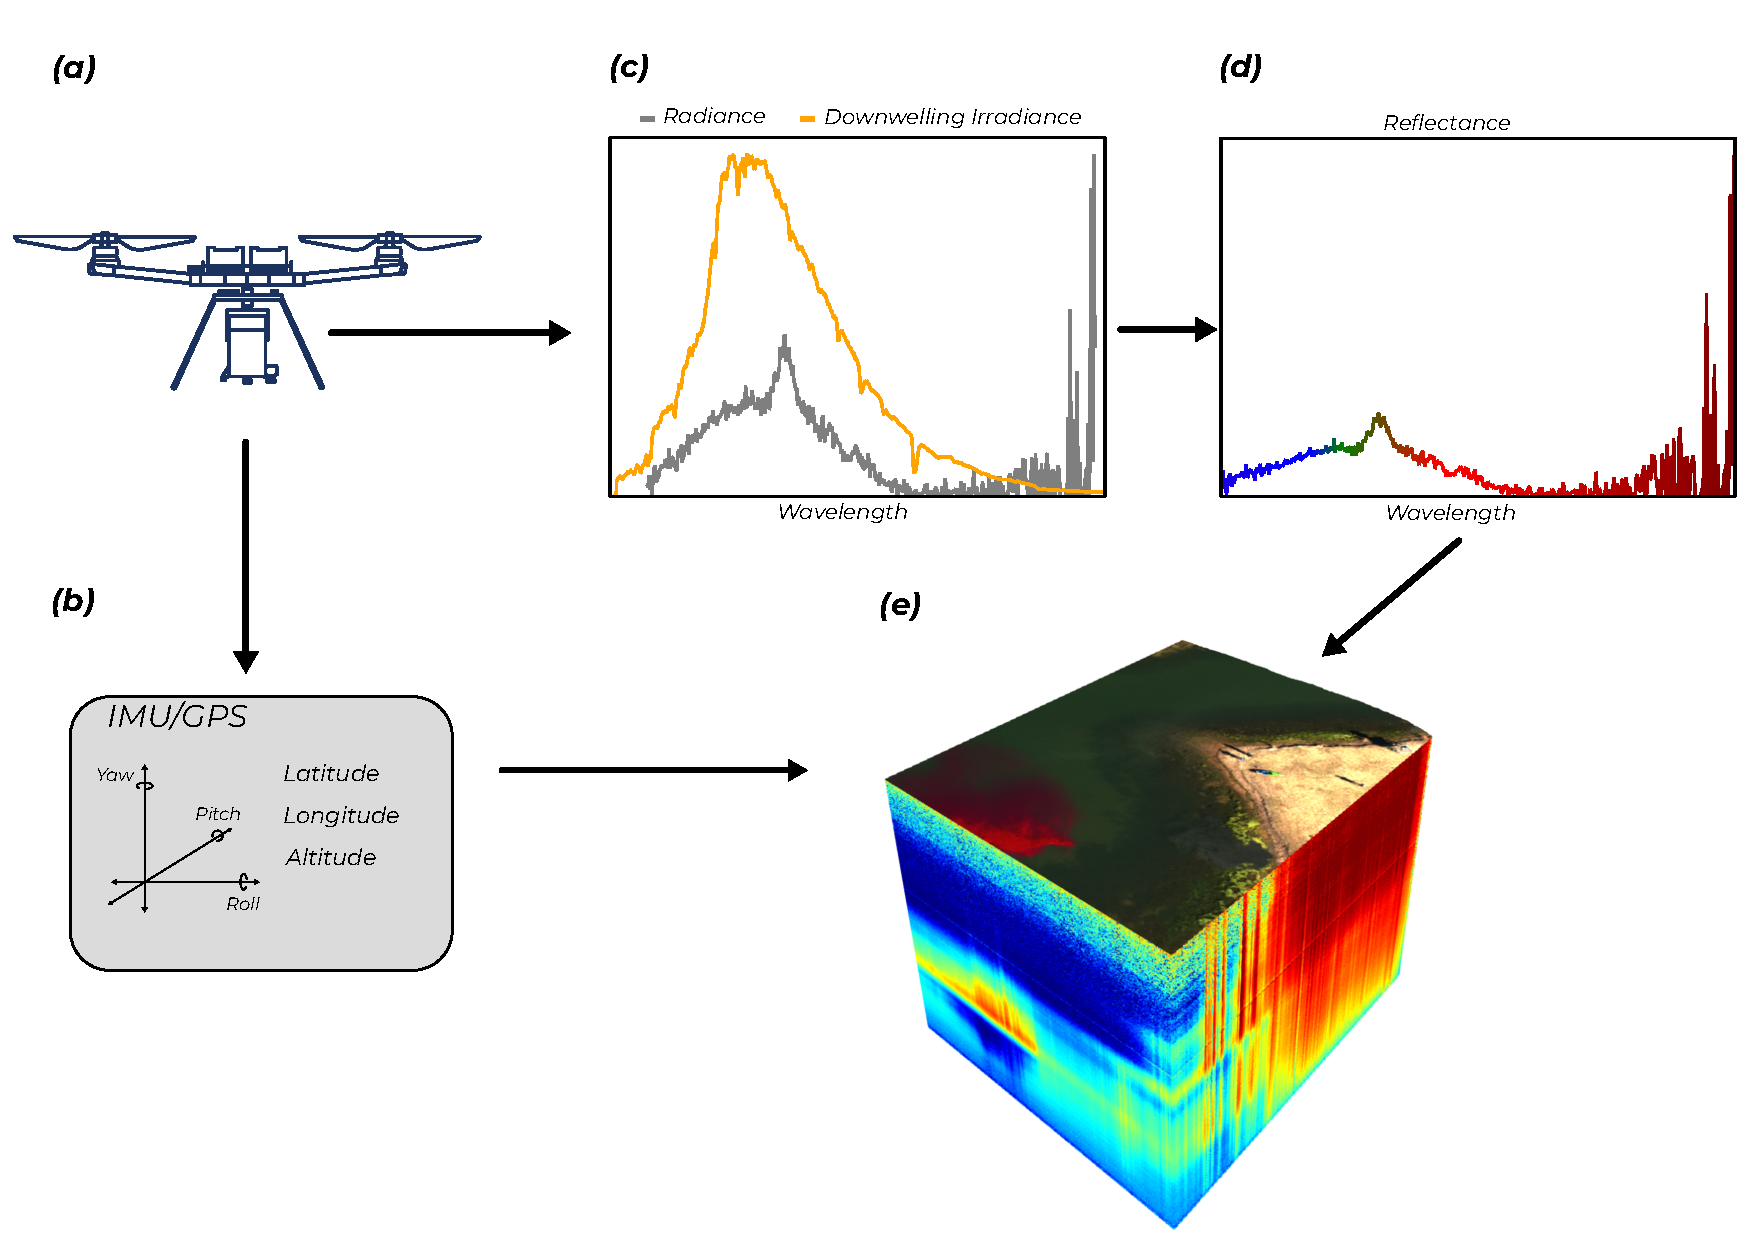
\includegraphics[width=0.85\columnwidth]{robot-team/georectification/pipeline-figure.pdf}
%   \caption{Visual representation of the HSI processing pipeline. HSI images from
%   the UAV (a) are georectified using position and orientation data from the
%   embedded GPS/IMU unit (b). Pixel radiance spectra are combined with
%   downwelling irradiance (c) to yield a reflectance spectrum for each pixel (d).
%   The result is a georectified reflectance data cube (e).}
%   \label{fig:hsi-pipeline}
% \end{figure}


\subsection{Georeferencing and Resampling}

The hyperspectral imager used on the UAV is different from a typical camera;
instead of capturing an image by sampling light across array of sensors, the
hyperspectral imager uses a pushbroom configuration. In this setup, a single
scan-line of pixels is captured by the sensor for each wavelength and an image
is formed as the drone flies along its route. This poses an interesting
challenge for georeferencing as each individual scanline must be transformed
independently. As the drone's path winds and turns, each scanline
is stretched and rotated based on the relative orientation of
the drone to the ground at the time of capture. This sampling geometry as well
as the relevant orientation angles are illustrated in Figure
\ref{fig:georectification}.

\begin{figure}[h]
  \centering
  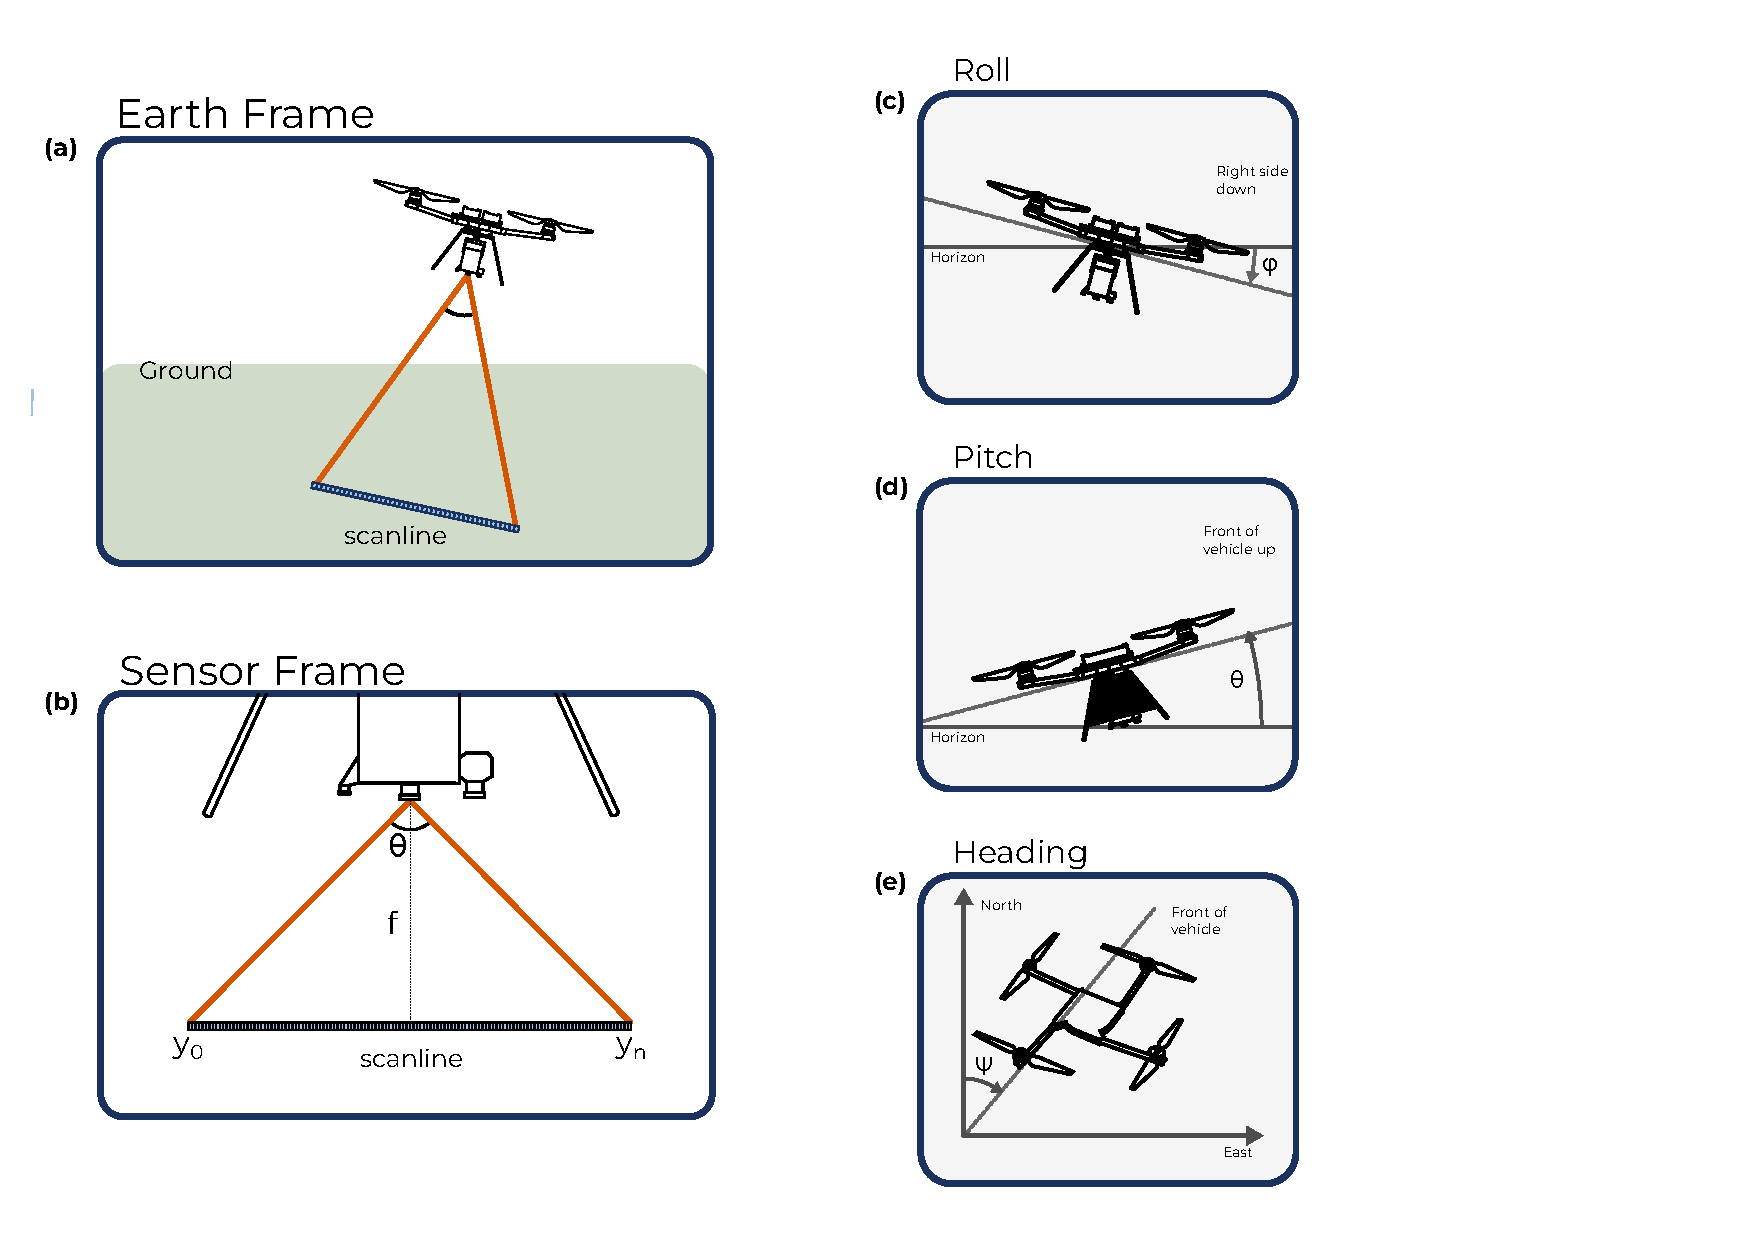
\includegraphics[width=0.95\columnwidth]{robot-team/georectification.pdf}
  \caption{Visual representation of sampling geometry for the UAV. (\textbf{a})
    the scan-line as seen from the Earth frame. (\text{b}) the HSI scan-line as
    represented in the frame of the sensor. (\textbf{d, d, e}) The angles
    describing the orientation of the drone in flight.}
  \label{fig:georectification}
\end{figure}

The GPS and IMU on the hyperspectral imager continuously capture the location $(\lambda,
\Phi, z)^T$  (longitude, latitude, altitude) of our drone as well it's
orientation defined by the angles $\phi$, $\theta$, and  $\psi$ (roll, pitch,
and heading). To georeference each pixel, we therefore must transform its
position from the frame of the sensor (measured in pixels relative to the
imager's sensor) first to the frame of the IMU used to measure the orientation,
then to the navigation frame (East, North, up), and finally to the ground frame. Let us
define the \textit{sensor} frame so that the scan-line falls upon the y axis. As
each scanline must be transformed independently, we can assign it an
x-coordinate of $0$ pixels. Lastly, if the viewing angle of the HSI is
$\theta_{\text{view}}$, then the coordinates of the i-th pixel,
$\mathbf{r}_i^{\text{sensor}}$, in the sensor frame are defined as in panel (b)
of Figure \ref{fig:georectification} to be
\begin{equation}
  \mathbf{r}_i^{\text{sensor}} = \left[ 0, y_i, f \right]^T
\end{equation}
where $y_i\in \left\{-\frac{(N-1)}{2},...,\frac{N-1}{2}\right\}$ and
$f=\frac{(N-1)/2}{\tan(\theta_{\text{view}}/2)}$ for $N$-total pixels per
scan-line. To align the sensor frame with the axes of
the IMU, we apply a sequence of rotation matrices defined using the measured
orientation angles (panels (c), (d), and (e) of Figure
\ref{fig:georectification}), denoted by
\begin{equation}
  \begin{aligned}
    &\mathbf{R}_{\text{sensor}}^{\text{IMU}}(\phi,\theta,\psi) = \\
    &\begin{bmatrix}
    \cos(\psi)\cos(\theta) & \cos(\psi)\sin(\theta)\sin(\phi)-\sin(\psi)\cos(\phi) & \cos(\psi)\sin(\theta)\cos(\phi)+\sin(\psi)\sin(\phi) \\
    \sin(\psi)\cos(\theta) & \sin(\psi)\sin(\theta)\sin(\phi)+\cos(\psi)\cos(\phi) & \sin(\psi)\sin(\theta)\cos(\phi)-\cos(\psi)\sin(\phi) \\
    -\sin(\theta) & \cos(\theta)\sin(\phi) & \cos(\theta)\cos(\phi)
     \end{bmatrix}.
  \end{aligned}
\end{equation}

Next, an orthogonal transformation is applied to transform from the IMU frame to
the navigation frame of the drone. This is important as the axes of the IMU and
the drone itself are not necessarily identical depending on how the IMU is
oriented on the HSI. For the UAV, this amounts to
\begin{equation}
  \mathbf{T}_{\text{IMU}}^{\text{DRONE}} = \begin{bmatrix}
    0 & 1 & 0 \\
    1 & 0 & 0 \\
    0 & 0 & -1
    \end{bmatrix}.
\end{equation}
At this stage, the pixel coordinates have been rotated into the frame of the
drone and must be rescaled from pixel units to meters. This is accomplished by
observing that panels (a) and (b) of Figure~\ref{fig:georectification} form
similar triangles with an shown in Figure~\ref{fig:s-geom}.

\begin{figure}[h]
  \centering
  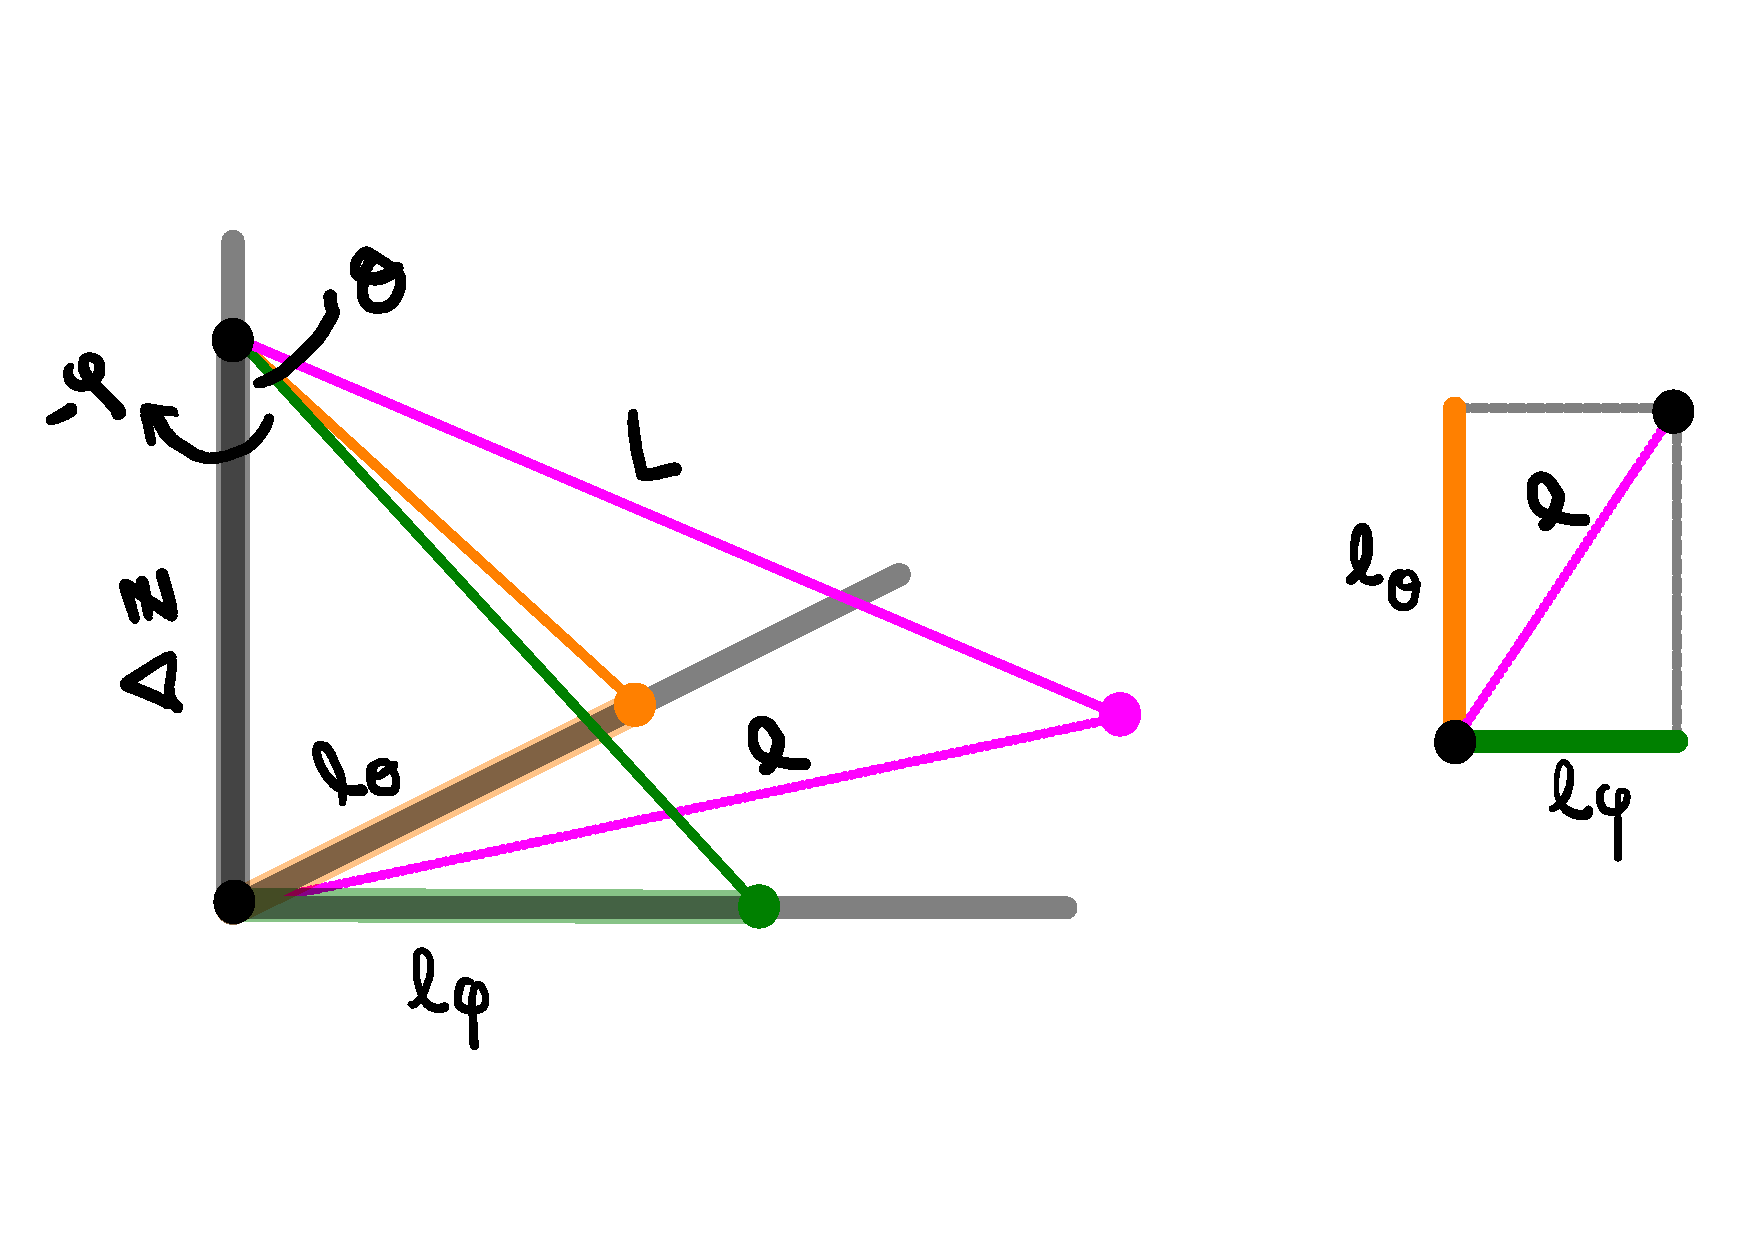
\includegraphics[width=0.6\columnwidth]{robot-team/scale-factor-geometry.pdf}
  \caption{At a height $\Delta z$, the position of an HSI pixel in the Earth
    frame depends on the roll $\theta$ and pitch $\phi$.}
  \label{fig:s-geom}
\end{figure}

For a height $\Delta z = z-z_{\text{ground}}$ above the ground, the distance $L$ from
the camera to an HSI pixel on the ground is
\begin{align*}
  L &= \sqrt{\Delta z^2 + \ell^2} \\
    &= \sqrt{\Delta z^2 + \Delta z^2\tan^2\theta + \Delta z^2\tan^2(-\phi)} \\
    &= \Delta z \sqrt{1 + \tan^2\theta + \tan^2\phi}
\end{align*}
leading to a scale factor
\begin{equation}
  s = \frac{L}{f} = \frac{\Delta z}{f}\sqrt{1 + \tan^2\theta + \tan^2\phi}.
\end{equation}

Finally, the coordinates of each pixel are translated using the position of the
drone in the chosen coordinate system. As the geometric transformations are
scaled to units of meters (by $s$), a coordinate transformation $f$ is applied to
obtain the position of the drone with respect to a local coordinate system such
as the Universal Transverse Mercator (UTM). Written all together, this becomes
\begin{equation}\label{eq:georec-eqn}
  \mathbf{r}_{i}^{\text{UTM}} =
  f_{\text{geo}}^{\text{UTM}}\begin{bmatrix}
    \lambda \\
    \Phi \\
    z_{\text{drone}}
  \end{bmatrix}_{\text{GPS}}^{\text{geo}} + s\mathbf{T}_{\text{IMU}}^{\text{DRONE}}\mathbf{R}_{\text{sensor}}^{\text{IMU}}(\theta, \phi, \psi)\begin{bmatrix}
    0 \\
    y_i \\
    f
  \end{bmatrix}^{\text{sensor}}
\end{equation}

The transformation from Equation~\ref{eq:georec-eqn} is applied \textit{in parallel}
to each scan-line to obtain the ground coordinates $\mathbf{r}_i=(x_i,
y_i,z_i)^T$ of each pixel. Finally, the resulting HSI is resampled to a
rectangular grid at a specified resolution by rounding each pixel's
coordinates to the desired accuracy and averaging all spectra that fall within the
same grid cell. Adjusting the final resolution of the georectified data cube
allows for optimization of compute time against spatial scale for real time
applications.

\subsection{Reflectance Conversion}

Once an HSI is georeferenced and resampled to the desired scale,
the downwelling irradiance spectrum measured during HSI acquisition is used to
convert the raw data from radiance to reflectance. This effectively normalizes
the HSI by \textit{dividing out} the incident light distribution making it possible
to compare spectra captured under variable lighting conditions. First,
the downwelling irraidance spectrum is loaded and interpolated to match the
wavelengths of the spectral bins of the hyperspectral imager. The reflectance at
pixel $(i,j)$ and wavelength $\lambda_k$ is then obtained by
\begin{equation}
  \rho_{ijk} = \frac{\pi L_{ijk}}{E_k}
\end{equation}
where $L_{ijk}$ denotes the original radiance pixel at wavelength bin $k$ and
$E_k$ denotes the downwelling irradiance at wavelength $\lambda_k$.

\begin{figure}[h]
  \vspace{-2cm}
  \centering
  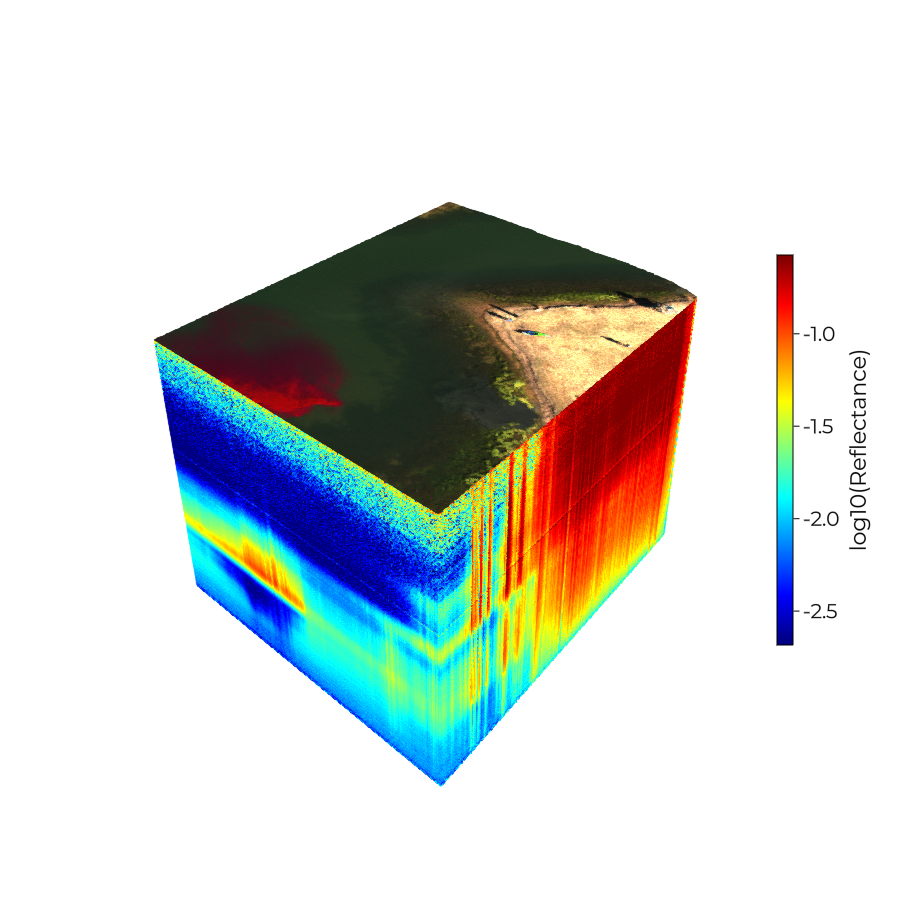
\includegraphics[width=0.55\columnwidth]{robot-team/georectification/demo-rectified-cube.png}
  \vspace{-1cm}
  \caption{Example of a georectified reflectance data cube. A pseudo color image is
    included at the top of the image showing what an observer would see from the
    perspective of the UAV. The log-10 reflectance is plotted at each wavelength
    bin along the z-axis. }
  \label{fig:sample-cube}
\end{figure}

Figure \ref{fig:sample-cube} illustrates an example of a georectified
reflectance data cube. The spectral signature corresponding to
a Rhodamine tracer dye released into the water is clearly visible in the front
left portion of the image.

\subsection{Timing Results}

This processing pipeline was implemented in the Julia programming language and
the associated code is accessible at \url{github.com/john-waczak/RobotTeam.jl}.
Using the package \texttt{BenchmarkTools.jl}, the time to load and georeference
HSI using the UAV processing computer for HSI with 371, 462, and 1000 scan-lines are
shown in Table~\ref{tab:georeference-times}.

\begin{table}[!hbt]
  \caption{Loading and georeferencing time as a function of number of scan-lines}
  \label{tab:georeference-times}
  \centering
  \begin{tabular}{cc}
    \hline
    \textbf{Number of scan lines}	& \textbf{Execution time (s)}\\
    \hline
    371		  &   0.161	\\
    462     &   0.197	\\
    1000    &   0.195  \\
    \hline
  \end{tabular}
\end{table}

The total processing time including resampling and conversion to reflectance as a
function of final resolution is shown in Figure~\ref{fig:regridding-timing} for
an HSI of initial size $1000\times 1600 \times 462$.

\begin{figure}[!hbt]
  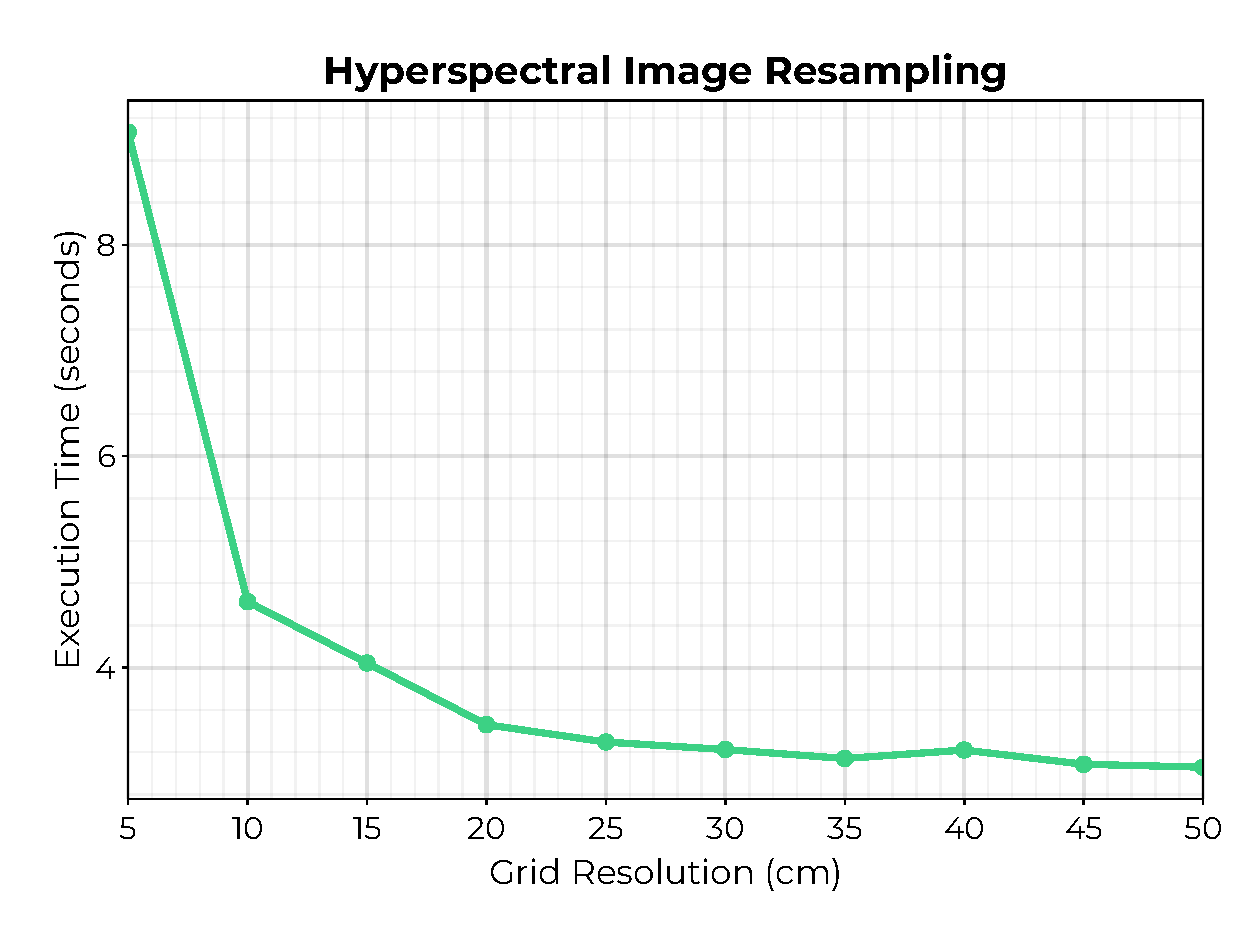
\includegraphics[width=0.85\columnwidth]{robot-team/georectification/regrid-timing.pdf}
  \caption{Timing results (in seconds) for resampling a 1000 scanline HSI as a function of output grid resolution.}
  \label{fig:regridding-timing}
\end{figure}

These timings indicate that processing an HSI to a final spatial resolution of
$20$ cm takes less than $4$ seconds which is comparable to the acquisition rate
of the hyperspectral imager. The key limitation of this implementation is the
assumption that the ground is flat. However, the studies in this dissertation
are focus specifically on imaging over the water where this approximation is
reasonable. For processing HSI collected over rough terrain, a digital elevation
map (DEM) can be used to augment the georectification process. Future iterations
of the drone can include small form-factor computers with integrated graphics
processing units (GPU) to accelerate these calculations. Here the problem of
georectification can be recast into a ray-tracing problem for each pixel
\cite{gpu-georect}.


\chapter{Distributed Sensor Networks for Real-Time Air Quality Assessment}\label{ch:air-network}

As outlined in Chapter~\ref{ch:intro}, air quality is a critical factor
affecting human health and well-being. Many pollutants such as Ozone, \ce{CO},
\ce{NO2}, \ce{SO2}, and volatile organic compounds contribute to poor air
quality. Among the variety of sources, particulate matter (PM) plays a
significant role and has
been linked to increased mortality by numerous studies
\cite{pm-mortality-six-cities, pm-mortality-2}. PM is particularly interesting
because its deleterious impacts on human health derive from both from its
composition \textit{and} its ability to penetrate into the tissues of the human
body. Beyond the obvious impact on lung health, PM pollution has been linked to
cardiovascular mortality \cite{pm-cardiovascular}, increased chronic kidney
disease \cite{pm-kidneys}, and recently, increased incidences of
neurodegenerative diseases like Alzheimer's \cite{pm-neurodegenerative,
  pm-neurodegenerative-2}. Therefore, the accurate assessment of PM exposure is
of paramount importance.

Considerable research efforts have focused on the development of accurate
measurement techniques for particulate matter. Unfortunately, most
reference-grade instruments remain prohibitively expensive, stunting our ability
to characterize spatial and temporal PM variations at scales relevant to dense
urban and suburban environments. Recently, a new class of low-cost PM sensors
based on optical particle counting has emerged. These sensors can be calibrated
against reference instruments using machine learning methods to improve
measurement accuracy and reduce inter-sensor variability
\cite{pm-calibration-lakitha}. Using these devices, our research group has
developed a family of low-cost monitors for real-time PM measurement. To date
over 100 monitors have been built and distributed across the Dallas Fort Worth
metroplex and other Texas cities.

In this chapter, we first describe physical measurement methods for PM. We then
describe the monitors developed by the MINTS research to provide real-time PM
measurements for a broad distribution of particle sizes. Finally, we describe
a comprehensive data pipeline developed for this dissertation which processes
real-time measurements measurement data and provides data visualization
dashboards. This system is designed using a variety of containerized open source
tools to guarantee reproducibility while ensuring the network can scale from
hundreds to thousands of sensors as they are built and deployed. Later
in Chapter~\ref{ch:havok} we analyze measurements collected
by sensors in this network to develop a physics-based method for outlier
detection and forecasting of PM time-series.

\section{Measurement of Particulate Matter}

Broadly speaking, instruments for measuring PM concentrations fall into one of
three categories:
\begin{itemize}
  \item \textbf{Federal Reference Methods} (FRM): These are methods which the US
    Environmental Protection Agency designate as the standard for PM measurement
    and may be used for assessing compliance with air quality regulations. The
    FRM for PM is \textit{gravimetric analysis} which collects size-selected
    particulate matter samples onto a polytetrafluoroethylene (PTFE) filter which are
    then carefully weighed to determine PM concentration by combining the sample
    mass with the sample flow rate \cite{pm-federal-reference-method}. Standard
    sizes are for PM 2.5 and PM 10 which correspond to particles with an
    aerodynamic diameter of $\leq 2.5$ $\mu m$ and $\leq 10$ $\mu m$, respectively.
  \item \textbf{Federal Equivalent Methods} (FEM): These measurement techniques
    include \textit{Beta Attenuation Monitors}  (BAM), \textit{Tapered Element
      Oscillating Ribbon} (TOEM) monitors, and \textit{Optical Particle
      Counters} (OPC) based on light scattering. FEM methods are also approved
    by the US EPA for ambient PM monitoring.
  \item \textbf{Low-cost Sensors}: These sensors are much less expensive than
    FRM and FEM systems but are not approved by the EPA for assessment of
    compliance with government regulations. Most low-cost sensors are simplified
    OPC systems.
\end{itemize}
The PM sensors described in this chapter fall into the low-cost OPC category.

\subsection{Optical Particle Counters}

Particulates scatter light according to their size and relevant physical
properties as described by Mie Scattering Theory for spherical dielectrics of
any radius. Optical particle
counters use light scattered off of particulates to estimate their size and
concentration. This method assumes particles are spherical and uses a
sufficiently slow flow rate so that, statistically speaking, particles enter the
sensing element individually. An example design for an OPC is shown below in
Figure~\ref{fig:opc-diagram}.

\begin{figure}[h]
  \centering
  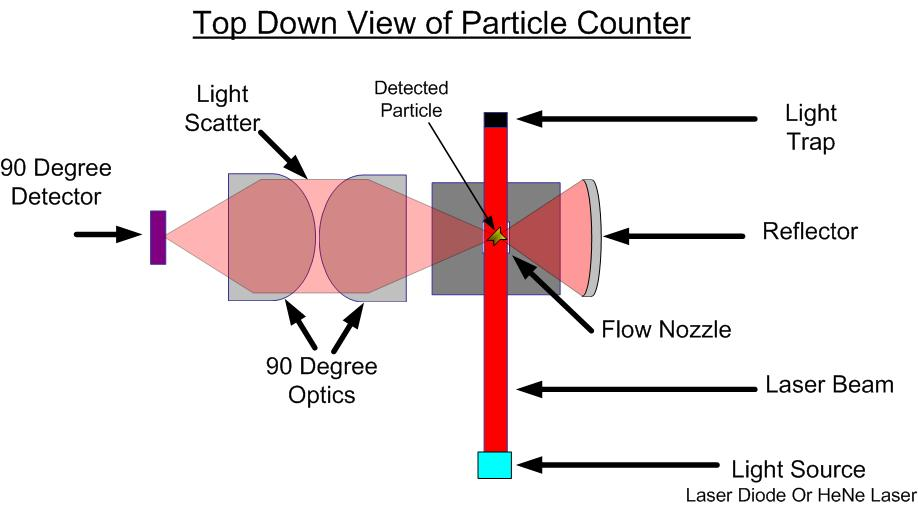
\includegraphics[width=0.7\columnwidth]{air-network/particle-counter.jpg}
  \caption{Optical particle counter: particulates are guided into the sensing
    element where a light source is then scattered off of the sample. This scattered
  light is then directed to detector. The inensity of scattered light is used to
distinguish particles by size. Image source: Morgan Polen, marked as public domain
(\url{https://en.wikipedia.org/wiki/File:Particlecounter.jpg}, accessed 2024-11-09). }
  \label{fig:opc-diagram}
\end{figure}

Particles are counted and sorted into distinct size bins based on the scattered
intensity with the detector oriented to limit the impact of index
of refraction on the scattered signal. For calibration,
most instruments use size-selected polystyrene spheres. Particle counts are then
converted into mass concentrations, for example PM 2.5 measured in $\mu g/m^3$.
This conversion is accomplished by assuming a constant particle density
consistent with observations for urban aerosols \cite{pm-density}.

An important consideration for OPCs is the impact of hygroscopic growth on
particle counts. When the humidity is sufficiently high, water tends to adsorb
onto particulates causing them to swell in size. Additionally, moistened
particulates may also agglomerate, coming together to form a larger particle
masses. This can significantly affect the accuracy of PM measurements by OPCs
leading to distortions in the estimated size distribution causing overestimation
of the true particulate mass. For this reason, FEM instruments using the OPC method
often include humidity control and heating elements. This significantly improves
the accuracy of sensor measurements but decreases the sampling rate to $1-10$
minutes per reading and increasing power consumption and instrument cost.
With the growing interest in low-cost OPC-based sensors, a variety of
corrections using local temperature and humidity data have also been suggested
\cite{opc-corrections}.

The current iteration of air quality monitors designed by the MINTS research
group utilize the Pierra Systems IPS7100 Intelligent Particle Sensor. This
device is capable of measuring PM concentrations at 1 Hz across 7 size bins
enabling concentration measurements for PM $0.1$, $0.3$, $0.5$, $1$, $2.5$, $5$,
and $10$. Estimation of ultra-fine particulates is made possible due to the
detectors $1$ MHz sampling rate. We note that the $0.1$ $\mu m$ size bin, is
extrapolated from the measured size distribution. An example of an individual
IPS7100 sensor is shown in Figure~\ref{fig:ips7100}.

\begin{figure}[!h]
  \vspace{-1cm}
  \centering
  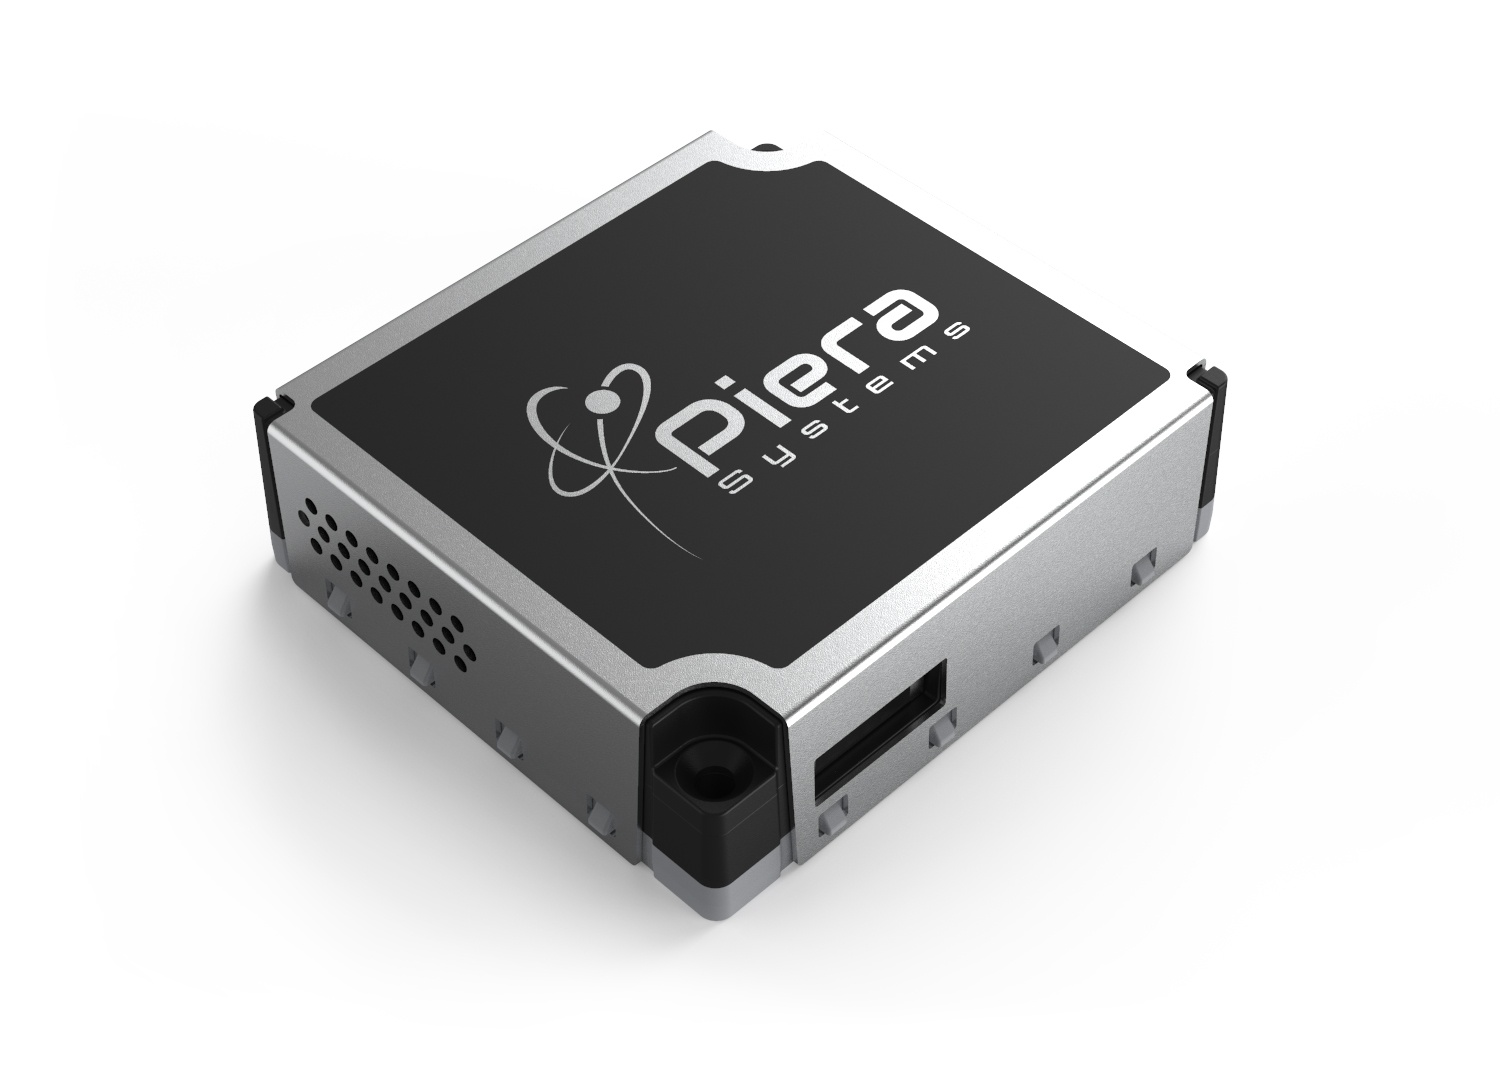
\includegraphics[width=0.4\columnwidth]{air-network/ips7100.jpg}
  \caption{The Pierra Systems IPS7100 Particulate Sensor.}
  \label{fig:ips7100}
\end{figure}

\section{A Low Cost Sensor Network For Air Quality Monitoring}


% The highly expensive cost to acquire, calibrate, and maintain reference grade
% air quality monitors makes it challenging to assess the importance of spatial
% and temporal variability on local air quality. Since factors such as weather,
% terrain, traffic, and the distribution of other sources can all effect local air
% quality, the development of low-cost sensing solutions is vital to address risks
% of poor air quality on local communities. To address this gap, we have developed
% a hierarchy of low-cost air quality monitors which we have deployed throughout
% the Dallas Fort-Worth (DFW) metroplex. In this section, we describe the relevant
% sensor types as well as a robust data processing and visualization pipeline
% developed to enable open access to high quality data.

\subsection{Sensor Nodes}

The sensor network is comprised of a combination of two types of nodes:
\textit{Central Nodes} and \textit{LoRa Nodes}. The central nodes are designed
to be deployed in locations with where dedicated power is available. Each
contains a variety of sensors including the IPS7100, VOCs,
\ce{CO2}, \ce{NO_X}, ionizing radiation, incident light intensity,
sound levels, as well as meteorological variables including temperature,
pressure, relative humidity, and dew point. The powered Central Nodes are
equipped with a cellular modem to facilitate data transfer from the field.


Each Central Node supports a collection of ~10 LoRa nodes (named for the
long rage wireless transmission protocol) which can be separated by distances up
to ~5 km or more if line of sight is established. These smaller sensors are self
powered using a combination of battery and solar cells, and each measures a
similar assortment of air quality parameters including particulate matter
concentrations, gas concentrations, and meteorological parameters. Designs for
the two node types are illustrated in Figure~\ref{fig:mints-nodes}.

\begin{figure}[!hbt]
  \begin{subfigure}{.5\textwidth}
    \centering
    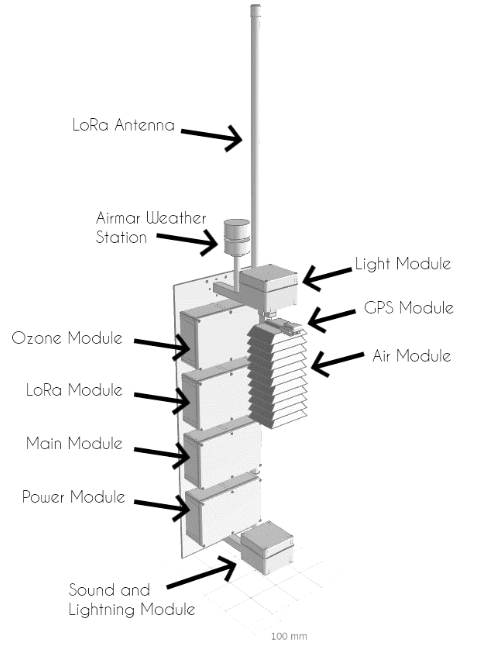
\includegraphics[width=.8\linewidth]{air-network/central-node.png}
    \caption{A 3d model of a Central Node}
  \end{subfigure}
  \begin{subfigure}{.5\textwidth}
    \centering
    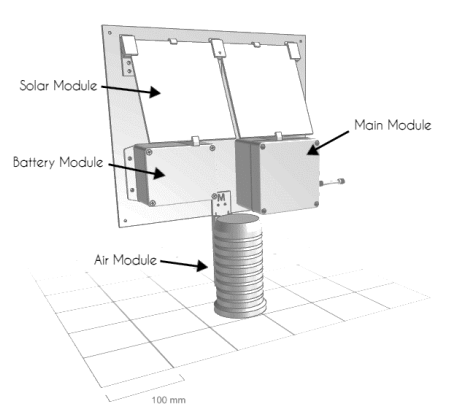
\includegraphics[width=.8\linewidth]{air-network/lora-node.png}
    \caption{A 3d model of a LoRa Node}
  \end{subfigure}
  \caption{Two types of nodes from the MINTS Air Quality network. Reproduced
    with permission from \cite{lakitha-thesis}}
  \label{fig:mints-nodes}
\end{figure}

Using the LoRaWAN protocol, Central and LoRa nodes form a low-power, wide-area
network through which data packets containing live measurements from each
LoRa node are transmitted to the nearest Central Node. The central nodes then
pass measurement data to a to a data processing backend using an MQTT
publish-subscribe model with their build-in cellular connection \cite{mqtt}.
Beginning in 2020, the first generation of nodes were built and installed as
shown in Figure~\ref{fig:sharedair-site}. In addition to sensor from MINTS, the
map also shows EPA reference sensors as well as live sensors from the PurpleAir network.

\begin{figure}[!hbt]
  \centering
  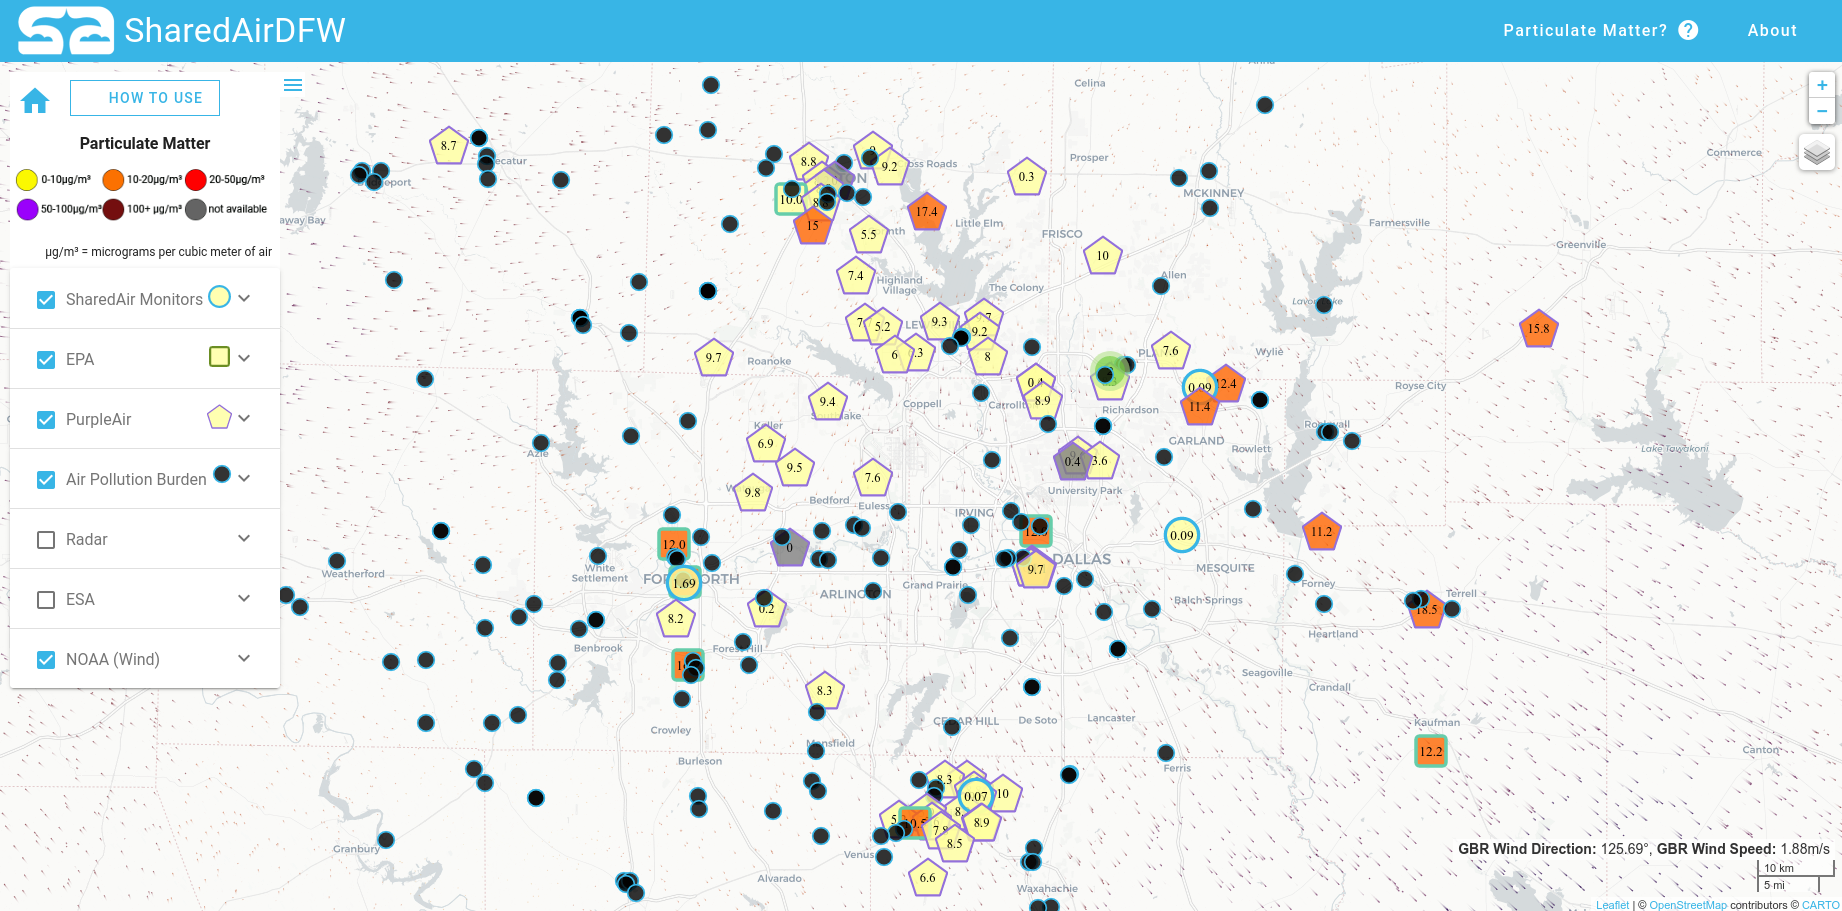
\includegraphics[width=0.85\columnwidth]{air-network/sharedairdfw-homepage.png}
  \caption{Interactive website displaying live sensor data on map. MINTS sensors
  are denoted with circular markers and additional data sources from EPA
  monitoring sites and PurpleAir monitors are included. Wind fields visualized
  using forecasts provided by NOAA.}
  \label{fig:sharedair-site}
\end{figure}


\subsection{The Data Pipeline}

To make real-time data available for public consumption and further analyses, a
containerized pipeline was implemented which combines a variety of open-source
data processing and visualization tools. \textit{Containerization} is a
method of encapsulating software together with
all of its dependencies, libraries, and configuration settings. Critically,
containerization makes software components such as databases and web servers
highly portable so that tools can be developed locally and then deployed to
remote systems.

Containers are defined using \textit{Dockerfiles} and can be networked together
with common data storage to achieve complex workflows. The pipeline developed
for the MINTS air quality network combines three containerized open-source tools:
\begin{itemize}
\item \textbf{NodeRed}: This tool developed by IBM allows the creation of
  data processing pipelines by defining directed acyclic graphs (DAGs)
  composed of individual processing nodes. This tool is utilized to subscribe to
  each sensor's MQTT topics and decode binary data packets into individual
  sensor measurements. Processed data are then injected by NodeRed into a
  time-series database. A key advantage of NodeRed is that the vast set of
  pre-implemented nodes which provde an easily maintainable, low-code data
  processing environment.
\item \textbf{InfluxDB}: This is a open source time-series database optimized
  for large cardinality datasets. By storing processed data in InfluxDB, we are
  able to provide queryable access to live and historic measurements.
\item \textbf{Grafana}: This tool is an visualization platform for
  creating interactive dashboards. Grafana is connected to InfluxDB to provide
  detailed, real-time displays for each sensor in the network. These dashboards
  visualize data from \textit{all} incoming measurements from each node in
  addition to the PM.
\end{itemize}

\begin{figure}[!h]
  \centering
  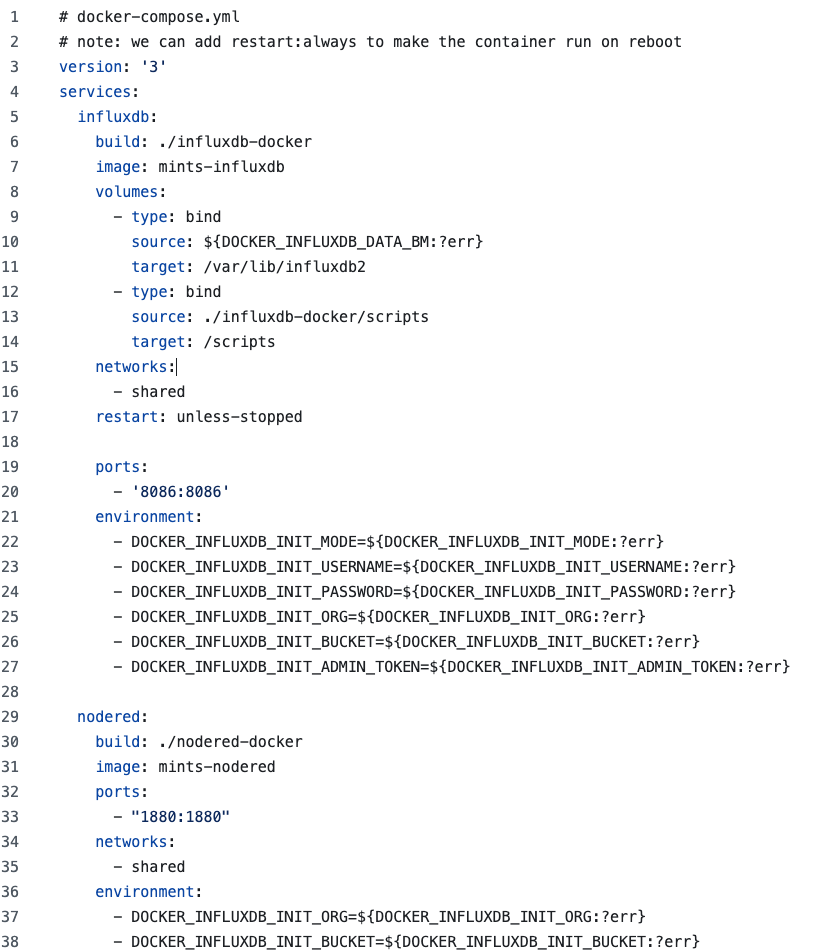
\includegraphics[width=0.95\columnwidth]{air-network/compose-snippet.png}
  \caption{Snippet of the \texttt{docker-compose.yml} file showing the
    combination of InfluxDB and NodeRed. Each individual container can define
    network ports, shared data volumes, and environment variables.}
  \label{fig:compose}
\end{figure}

Container orchestration is accomplished using YAML files like the examples shown
in Figure~\ref{fig:compose}




\begin{figure}[!h]
  \centering
  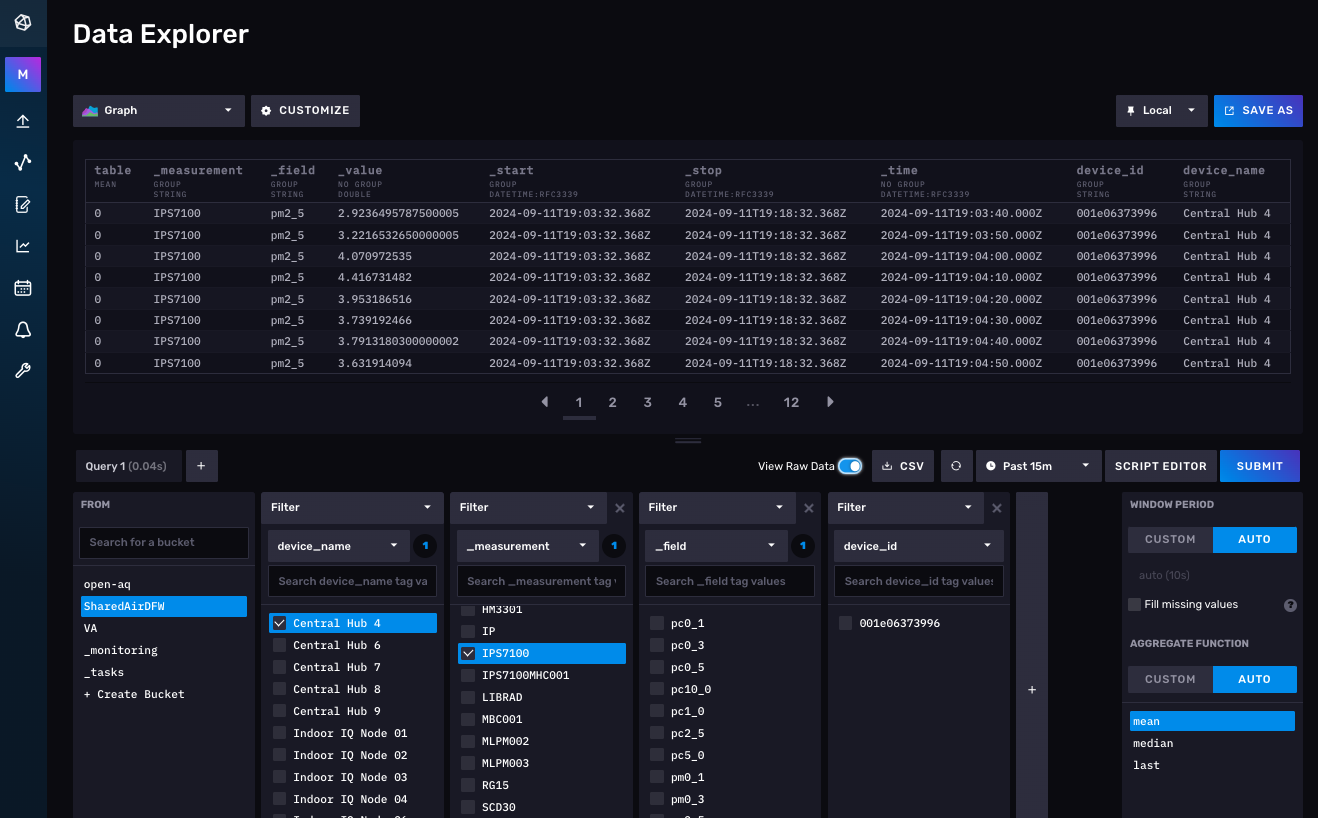
\includegraphics[width=0.95\columnwidth]{air-network/influxdb.png}
  \caption{A view of the time series data accessible from the InfluxDB database.
  Each sensor is assigned a unique device name. Time-series for individual
  sensor measurements can be identified by the sensor name and the specific
  measurement.}
  \label{fig:influxdb}
\end{figure}




\begin{figure}[!h]
  \centering
  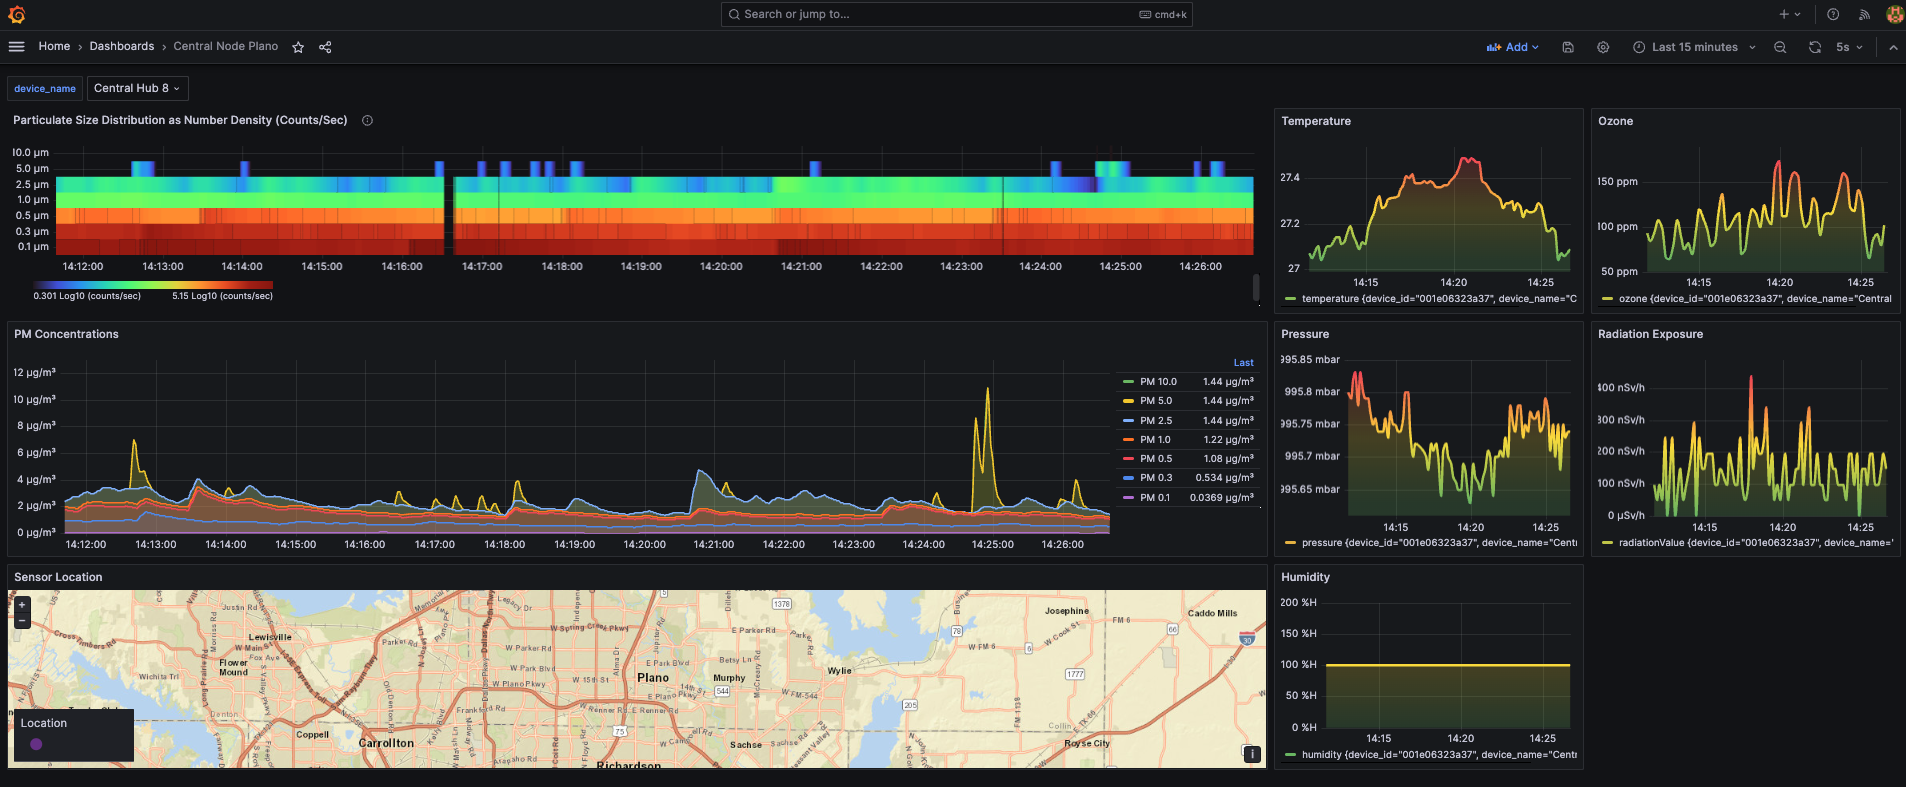
\includegraphics[width=0.95\columnwidth]{air-network/grafana.png}
  \caption{Example grafana dashboard}
  \label{fig:grafana}
\end{figure}





\textbf{Open Storage Network}: With help from Dr. Chris Simmons, we have
  developed a pipeline for long term data storage utilizing the Open Storage
  Network to provide open access to historic sensor data stored in the popular
  S3 format.
 




\chapter{Characterizing Water Quality with Autonomous Robotic Teams and Supervised Learning}\label{ch:robot-team-supervised}


Inland waters pose a unique challenge for water quality monitoring by remote
sensing techniques due to their complicated spectral features and
small-scale variability. At the same time, collecting the reference data
needed to calibrate remote sensing data products is both time consuming and
expensive. In this study, we present the further development of a robotic
team composed of an uncrewed surface vessel (USV) providing in situ
reference measurements and an unmanned aerial vehicle (UAV) equipped with a
hyperspectral imager. Together, this team is able to address the limitations
of existing approaches by enabling the simultaneous collection of
hyperspectral imagery with precisely collocated in situ data. We showcase
the capabilities of this team using data collected in a northern Texas pond
across three days in 2020. Machine learning models for 13~variables are
trained using the dataset of paired in situ measurements and coincident
reflectance spectra. These models successfully estimate physical variables
including temperature, conductivity, pH, and turbidity as well as the
concentrations of blue--green algae, colored dissolved organic matter
(CDOM), chlorophyll a, crude oil, optical brighteners, and the ions
$\mathrm{Ca}^{2+}$, $\mathrm{Cl}^{-}$, and $\mathrm{Na}^{+}$. We extend the
training procedure to utilize conformal prediction to estimate 90\%
confidence intervals for the output of each trained model. Maps generated by
applying the models to the collected images reveal small-scale spatial
variability within the pond. This study highlights the value of combining
real-time, in situ measurements together with hyperspectral imaging for the
rapid characterization of water composition.


\textcolor{red}{
  Make sure to add sentence about the publications where this appears, e,g
  \cite{robot-team-1, robot-team-2}
}

\section{Motivation}


For decades, remote sensing imagery has been used for environmental monitoring, with applications ranging from resource mapping, land type classification, and urban growth assessment to wildfire monitoring, natural disaster tracking, and many more~\cite{melesse2007remote, joyce2009review}. Among these applications, the retrieval of water quality variables from remote sensing imagery remains challenging due to the difficulty of obtaining in situ reference data coincident with available satellite imagery. Traditional approaches to obtain these data have relied on serendipitous satellite passes over fixed sensing sites or sensor-equipped vessels. As a consequence, curating comprehensive datasets can require decades of observations~\cite{aurin2018remote, ross2019aquasat}. This poses a significant challenge for assessing natural and anthropogenic changes to water composition in real time, for example, during oil spills \cite{fingas2017review}.

Where remote sensing imagery and in situ measurements have been combined, studies have demonstrated successful extraction of optically active water quality variables such as colored dissolved organic matter (CDOM), chlorophyll-a, and suspended sediment concentrations by using combinations of spectral bands \cite{remote-sensing-finland,bonansea2015using, absalon2023detection}. These approaches can be further augmented by machine learning methods, which consist of nonlinear and non-parametric models designed to learn representations of functions directly from data \cite{lary2010artificial}. For example, Petersen et al. utilized a deep neural network to successfully estimate blue--green algae, chlorophyll-a, CDOM, dissolved oxygen, specific conductance, and turbidity from a fused dataset of Landsat-8 and Sentinel-2 imagery \cite{peterson2020deep}. Other methods such as support vector machines and decision trees have also been successfully applied to retrieve water quality parameters from remote sensing imagery \cite{belgiu2016random,sagan2020monitoring}. However, the low spatial and spectral resolution of available multiband remote sensing satellites makes it difficult to analyze inland waters with small spatial features and complicated spectral signatures. 

Advances in multispectral and hyperspectral imaging technology have led to considerable reductions in size, making it possible to incorporate these cameras into the payloads of autonomous aerial vehicles (UAVs) \cite{hruska2012radiometric}. Flying at low altitudes enables the collection of centimeter-scale imagery whilst limiting the need for complicated atmospheric corrections to account for scattering by atmospheric aerosols and gasses \cite{adao2017hyperspectral, banerjee2020uav}. Already, UAVs equipped with multispectral and hyperspectral imagers are being used in a variety of domains to great effect, including for biomass estimation, forest management, precision agriculture, and, recently, water quality monitoring \cite{adao2017hyperspectral, padua2017uas,arroyo2019implementation,kurihara2020unmanned, ehmann2019monitoring}. Despite the superior spectral and spatial resolution enabled by UAV platforms, these improvements alone do not address the limited spatial coverage of the in situ reference data used for the associated water composition retrieval. For instance, Lu et al. used a UAV-born hyperspectral imager to develop machine learning models for the inversion of chlorophyll-a and suspended solids using samples from 33 fixed locations \cite{lu2021retrieval}. Similarly, Zhang et al. utilized a UAV equipped with a hyperspectral imager to estimate water quality parameters by collecting imagery coincident with samples taken from 18 sampling sites \cite{zhang2022selection}. In both of these examples, the collection of in situ reference data remains the key challenge for the application of UAV systems to water quality quantification.

To address this gap and enable comprehensive, real-time evaluation of water composition, we have developed a robotic team comprised of an autonomous uncrewed surface vessel (USV) equipped with a collection of reference grade instruments together with a UAV carrying a hyperspectral imager. By incorporating reference instruments on a maneuverable USV platform, we are able to rapidly collect large volumes of water quality data for a comprehensive suite of physical, biochemical, and chemical variables that are precisely collocated with spectra captured by the UAV. Critically, the USV enables the collection of reference data with significantly improved spatial resolution compared to other approaches. In our previous work, we introduced this paradigm and described how in situ measurements collected by the USV can be used to provide the ground-truth data for machine learning models that map the reflectance spectra captured by the hyperspectral imager to the desired water quality variables \cite{robot-team-1}.

The main objective of this study is to expand on our previous work in three new ways: The first is to explore the breadth of water quality variables that can be inferred from collected hyperspectral imagery. With the goal of comprehensive measurement in mind, we demonstrate the ability to accurately predict physical variables such as temperature, conductivity, pH, and turbidity as well as biochemical constituents, including blue--green algae pigments, CDOM, and chlorophyll-a, in addition to concentrations of crude oil, optical brighteners, and a variety of ions. The second addition is to demonstrate that observations from separate collections can effectively be combined by carefully accounting for variability in the viewing and illumination geometries of the scene. Finally, we expand our machine learning approach to take advantage of the considerable volume of collected data in order to determine reliable confidence intervals for each predicted parameter using conformal prediction.




\section{Supervised Learning}
\subsection{Decision Trees}
\subsection{Ensemble Learning and Random Forests}
\subsection{Cross Validation}
\subsection{Conformal Prediction}
Conformalizing Quantile Regression
Conformalizing Scalar Uncertainty Estimates
\subsection{Permutation Importance}



\section{Rapid Processing of Hyperspectral Imagery}
\subsection{Georectification}
\subsection{Reflectance Conversion}
\subsection{Implementation and Timing Results}



\section{Study Overview}

 The robotic team presented in this study consists of two key sensing sentinels: an uncrewed surface vessel (USV) used to collect in situ reference measurements and an unmanned aerial vehicle (UAV) for performing rapid, wide-area surveys to gather remote sensing data products. Both platforms are coordinated using open-source QGroundControl version 4.0.11 software for flight control and mission planning and are equipped with high-accuracy GPS and INS such that all data points collected are uniquely geolocated and time-stamped~\cite{qgroundcontrol}. Both the USV and UAV include long-range Ubiquiti 5 GHz LiteBeam airMAX WiFi to enable streaming of data products to a ground station with network-attached storage to provide redundancy.

\subsection{USV: In Situ Measurements}

The USV employed in the robot team is a Maritime Robotics Otter equipped with an in situ sensing payload consisting of a combination of Eureka Manta+40 multiprobes. These sensors include fluorometers, ion-selective electrodes, and other physical sensors and are mounted on the underside of the boat as illustrated in Figure~\ref{fig:boat-components}. Together, this sensor array enables the collection of comprehensive near-surface measurements including colored dissolved organic matter (CDOM), crude oil, blue--green algae (phycoerythrin and phycocyanin), chlorophyll-a, $\mathrm{Na^+}$, $\mathrm{Ca^{2+}}$, $\mathrm{Cl^-}$, temperature, conductivity, and many others. The full list of measurements utilized in this study is outlined in Table~\ref{tab:sensors} and is categorized into four distinct types: physical measurements, ion measurements, biochemical measurements, and chemical measurements. Additionally, the USV is equipped with an ultrasonic weather monitoring sensor for measuring air speed and direction as well as a BioSonics MX Aquatic Habitat Echosounder sonar, which are not explored in this study.

\begin{figure}[H]
\hspace{-6pt}\includegraphics[width=\columnwidth]{robot-team-supervised/materials-and-methods/annotated-boat.pdf}
\caption{Configuration of the USV: (\textbf{a}) Frontal view of the USV showing the Eureka Manta+40 multiprobes mounted on the underside of the boat. (\textbf{b}) The USV deployed in the water.\label{fig:boat-components}}
\end{figure}

As shown in Table~\ref{tab:sensors}, the physical measurements and ion sensors
are largely based on different electrode configurations, while the chemical and
biochemical measurements are all optically significant in UV and visible light,
enabling their determination by fluorometry
\cite{de2007ion,trees2002fluorometric,tillman2017evaluation}. The pigments
phycoerythrin and phycocyanin are used to determine the blue--green algae
content, which together with chlorophyll-a enables us to assess the distribution
of photosynthetic life in the pond~\cite{Brient2008APP, boyer2009phytoplankton}.
In addition, we also measured the concentration of colored dissolved organic
matter (CDOM), which impacts light penetration and serves as a primary source of
bioavailable carbon. Crude oil (natural petroleum) and optical brightener
concentrations are also measured with fluorometers and are relevant for
identifying sources of industrial contamination, natural seepage, and sewage
\cite{brown2003review,cao2009evaluation}.

\begin{sidewaystable}[p!]
  \caption{In situ reference sensors utilized in this study.}
  \label{tab:sensors}
  \begin{center}
    \begin{tabular}{ccccc} \hline
      \textbf{Sensor}	& \textbf{Units} & \textbf{Resolution} & \textbf{Sensor Type} & \textbf{Target Category}\\ \hline
      Temperature & $^{\circ}$C & 0.01 & Thermistor & Physical \\
      Conductivity & $\mu$S/cm & 0.01 & Four-Electrode Graphite Sensor & Physical  \\
      pH & logarithmic (0--14) & 0.01 & Flowing-Junction Reference Electrode & Physical \\
      Turbidity & FNU & 0.01 & Ion-Selective Electrode & Physical \\
      $\mathrm{Ca^{2+}}$ & mg/L & 0.1 & Ion-Selective Electrode & Ions \\
      $\mathrm{Cl^-}$ & mg/L & 0.1 & Ion-Selective Electrode & Ions \\
      $\mathrm{Na^+}$ & mg/L & 0.1 & Ion-Selective Electrode & Ions \\
      Blue--Green Algae (phycoerythrin) & ppb & 0.01 & Fluorometer & Biochemical \\
      Blue--Green Algae (phycocyanin) & ppb & 0.01  & Fluorometer & Biochemical \\
      CDOM & ppb & 0.01 & Fluorometer & Biochemical \\
      Chlorophyll a & ppb & 0.01 & Fluorometer & Biochemical \\
      Optical Brighteners & ppb & 0.01 & Fluorometer & Chemical \\\
      Crude Oil & ppb & 0.01 & Fluorometer & Chemical
    \end{tabular}
  \end{center}
\end{sidewaystable}


The inclusion of optically inactive variables such as conductivity, pH, and ion concentrations was motivated by a desire to be comprehensive. Multiple studies have classified inland water bodies according to their ionic compositions \cite{piper1944graphic, dordoni2023preliminary}. Other research indicates that the structure of dissolved organic matter is affected by changes in pH and cation concentration~\cite{pace2012ph}. Therefore, changes in physical parameters and ionic content can be expected to be related to the observed distribution of optically active variables in the water. It is therefore reasonable to expect that these parameters may be estimated from hyperspectral images at a given site.


\subsection{UAV: Hyperspectral Data Cubes}

A Freefly Alta-X autonomous quadcopter was used as a UAV platform for the robotic team. The Alta-X is specifically designed to carry cameras and has a payload of up to 35~lbs. We equipped the UAV with a Resonon Pika XC2 visible+near-infrared (VNIR) hyperspectral imager. For each image pixel, this camera samples 462 wavelengths ranging from 391 to 1011 nm.  Additionally, the UAV includes an upward facing Ocean Optics UV-Vis-NIR spectrometer with a cosine corrector to capture the incident downwelling irradiance spectrum. Data collection by the hyperspectral imager is controlled by an attached Intel NUC small-form-factor computer. A second processing NUC is also included for onboard georectification and generation of data products. The collected hyperspectral images (HSIs) are stored locally on a solid state drive that is simultaneously mounted by the processing computer. The configuration of the drone is shown in Figure~\ref{fig:drone-components}.

\begin{figure}[H]
\vspace{-0.3in}
\hspace{-16pt}\includegraphics[width=\columnwidth]{robot-team-supervised/materials-and-methods/annotated-drone.pdf}
\vspace{-0.2in}
\caption{Configuration of the UAV: (\textbf{a}) The hyperspectral imager and acquisition computer. (\textbf{b}) The assembled UAV with secondary processing computer and (upward facing) downwelling irradiance spectrometer. \label{fig:drone-components}}
\end{figure} 

To effectively utilize the spectra collected by our UAV, we must account for the variability of the incident light that illuminates the water and transform the raw hyperspectral data cubes from their native imaging reference frame to a chosen coordinate system compatible with the data collected by the USV. This procedure is illustrated in Figure~\ref{fig:hsi-pipeline}.

\begin{figure}[H]
%\centering
\vspace{-0.3in}
\hspace{-6pt}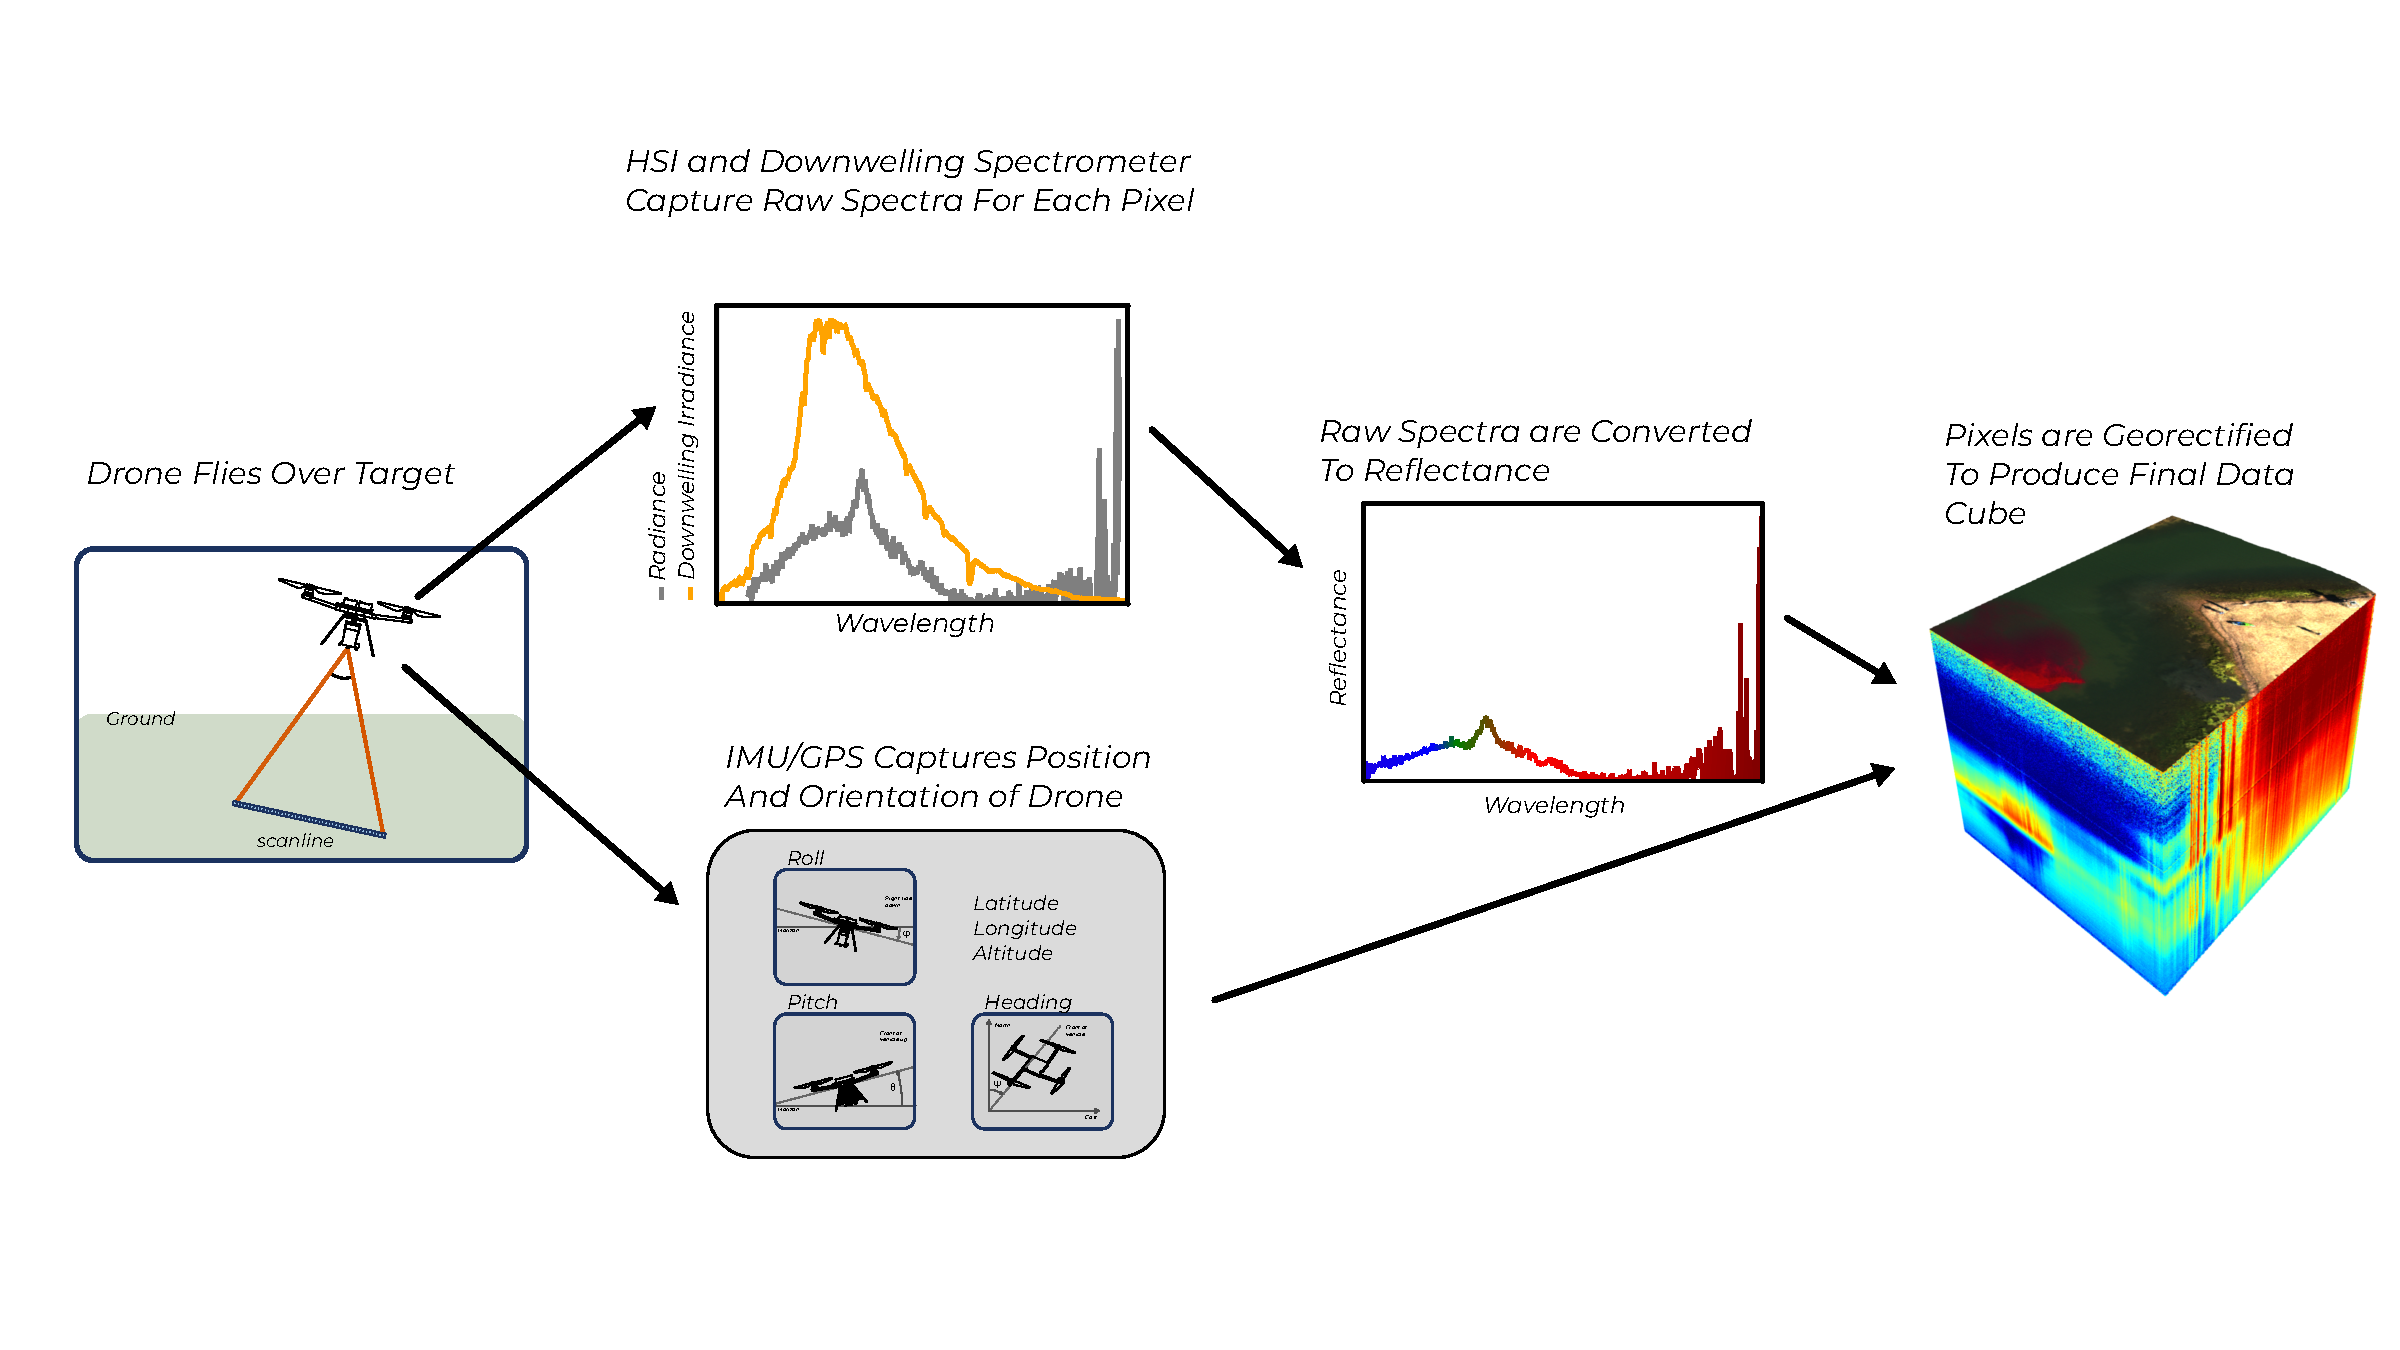
\includegraphics[width=14cm]{robot-team-supervised/materials-and-methods/pipeline-figure-2.pdf}
\vspace{-0.4in}
\caption{Hyperspectral image processing: Hyperspectral data cubes are collected one scan-line at a time (left). By utilizing downwelling irradiance spectra, we convert each pixel from spectral radiance to reflectance. By using orientation and position data from the on-board GPS and INS, we georeference each pixel to assign it a latitude and longitude on the ground. The final data product is the georectified hyperspectral reflectance data cube (right) visualized as a pseudo-color image with reflectance  as a function of wavelength along the z-axis.\label{fig:hsi-pipeline}}
\end{figure}  

The hyperspectral imager utilized in our robot team is in a so-called pushbroom configuration: that is, each image captured by the drone is formed one scan line at a time as the UAV flies. Each scan line consists of 1600 pixels, for which incoming light is diffracted into 462 wavelength bins. In the collection software, a regular cutoff of 1000 lines is chosen so that each resulting image forms an array of size 462 $\times$ 1600 $\times$ 1000 called a hyperspectral data cube. Initially, the captured spectra are in units of spectral radiance (measured in microflicks); however, this does not account for the variability of incident light illuminating the water. To this end, we convert the hyperspectral data cubes into units of reflectance by utilizing the skyward-facing downwelling irradiance spectrometer. When the camera is normal to the water surface, the reflectance is given by
\begin{equation}
    R(\lambda) = \pi L(\lambda)/E_d(\lambda)
\end{equation}
where $L$ is the spectral radiance, $E_d$ is the downwelling irradiance, and a factor of $\pi$ steradians results from assuming the water surface is Lambertian (diffuse) \cite{ruddick2019review}. 

Having converted the hyperspectral data cube to units of reflectance, we must also georeference each pixel into a geographic coordinate system so that each image pixel can be assigned a latitude and longitude corresponding to the location on the ground from which it was sampled. During our three surveys, the UAV was flown at an altitude of approximately %Please ensure meaning has been retained. 
50 m above the water. At this scale, the surface is essentially flat, so the hyperspectral data cube can be reliably georectified without the need for an on-board digital elevation map (DEM). We adopt the approach outlined in \cite{muller2002program, baumker2001new, mostafa2000multi} whereby each scan line is georeferenced using the known field of view (30.8$^\circ$) together with the position and orientation of the UAV as provided by the on-board GPS/INS. After a sequence of coordinate transformations, the pixel coordinates are obtained in the relevant UTM zone (in meters). The resulting image is then re-sampled to a final output resolution. For these collections, a resolution of 10 cm was utilized; however, this can be adjusted to optimize the processing time and final resolution for real-time applications. Finally, the UTM pixel coordinates obtained are transformed to latitude and longitude for easy comparison with in situ data collected by the USV. The final result is a georectified hyperspectral reflectance data cube. In Figure~\ref{fig:hsi-infographic}, we visualize one such data cube, highlighting a selection of exemplar pixel spectra as well as the incident downward irradiance spectrum. A pseudo-color image is generated (plotted on the top of the data cube) to illustrate the scene.

\begin{figure}[H]
\centering
\vspace{-0.1in}
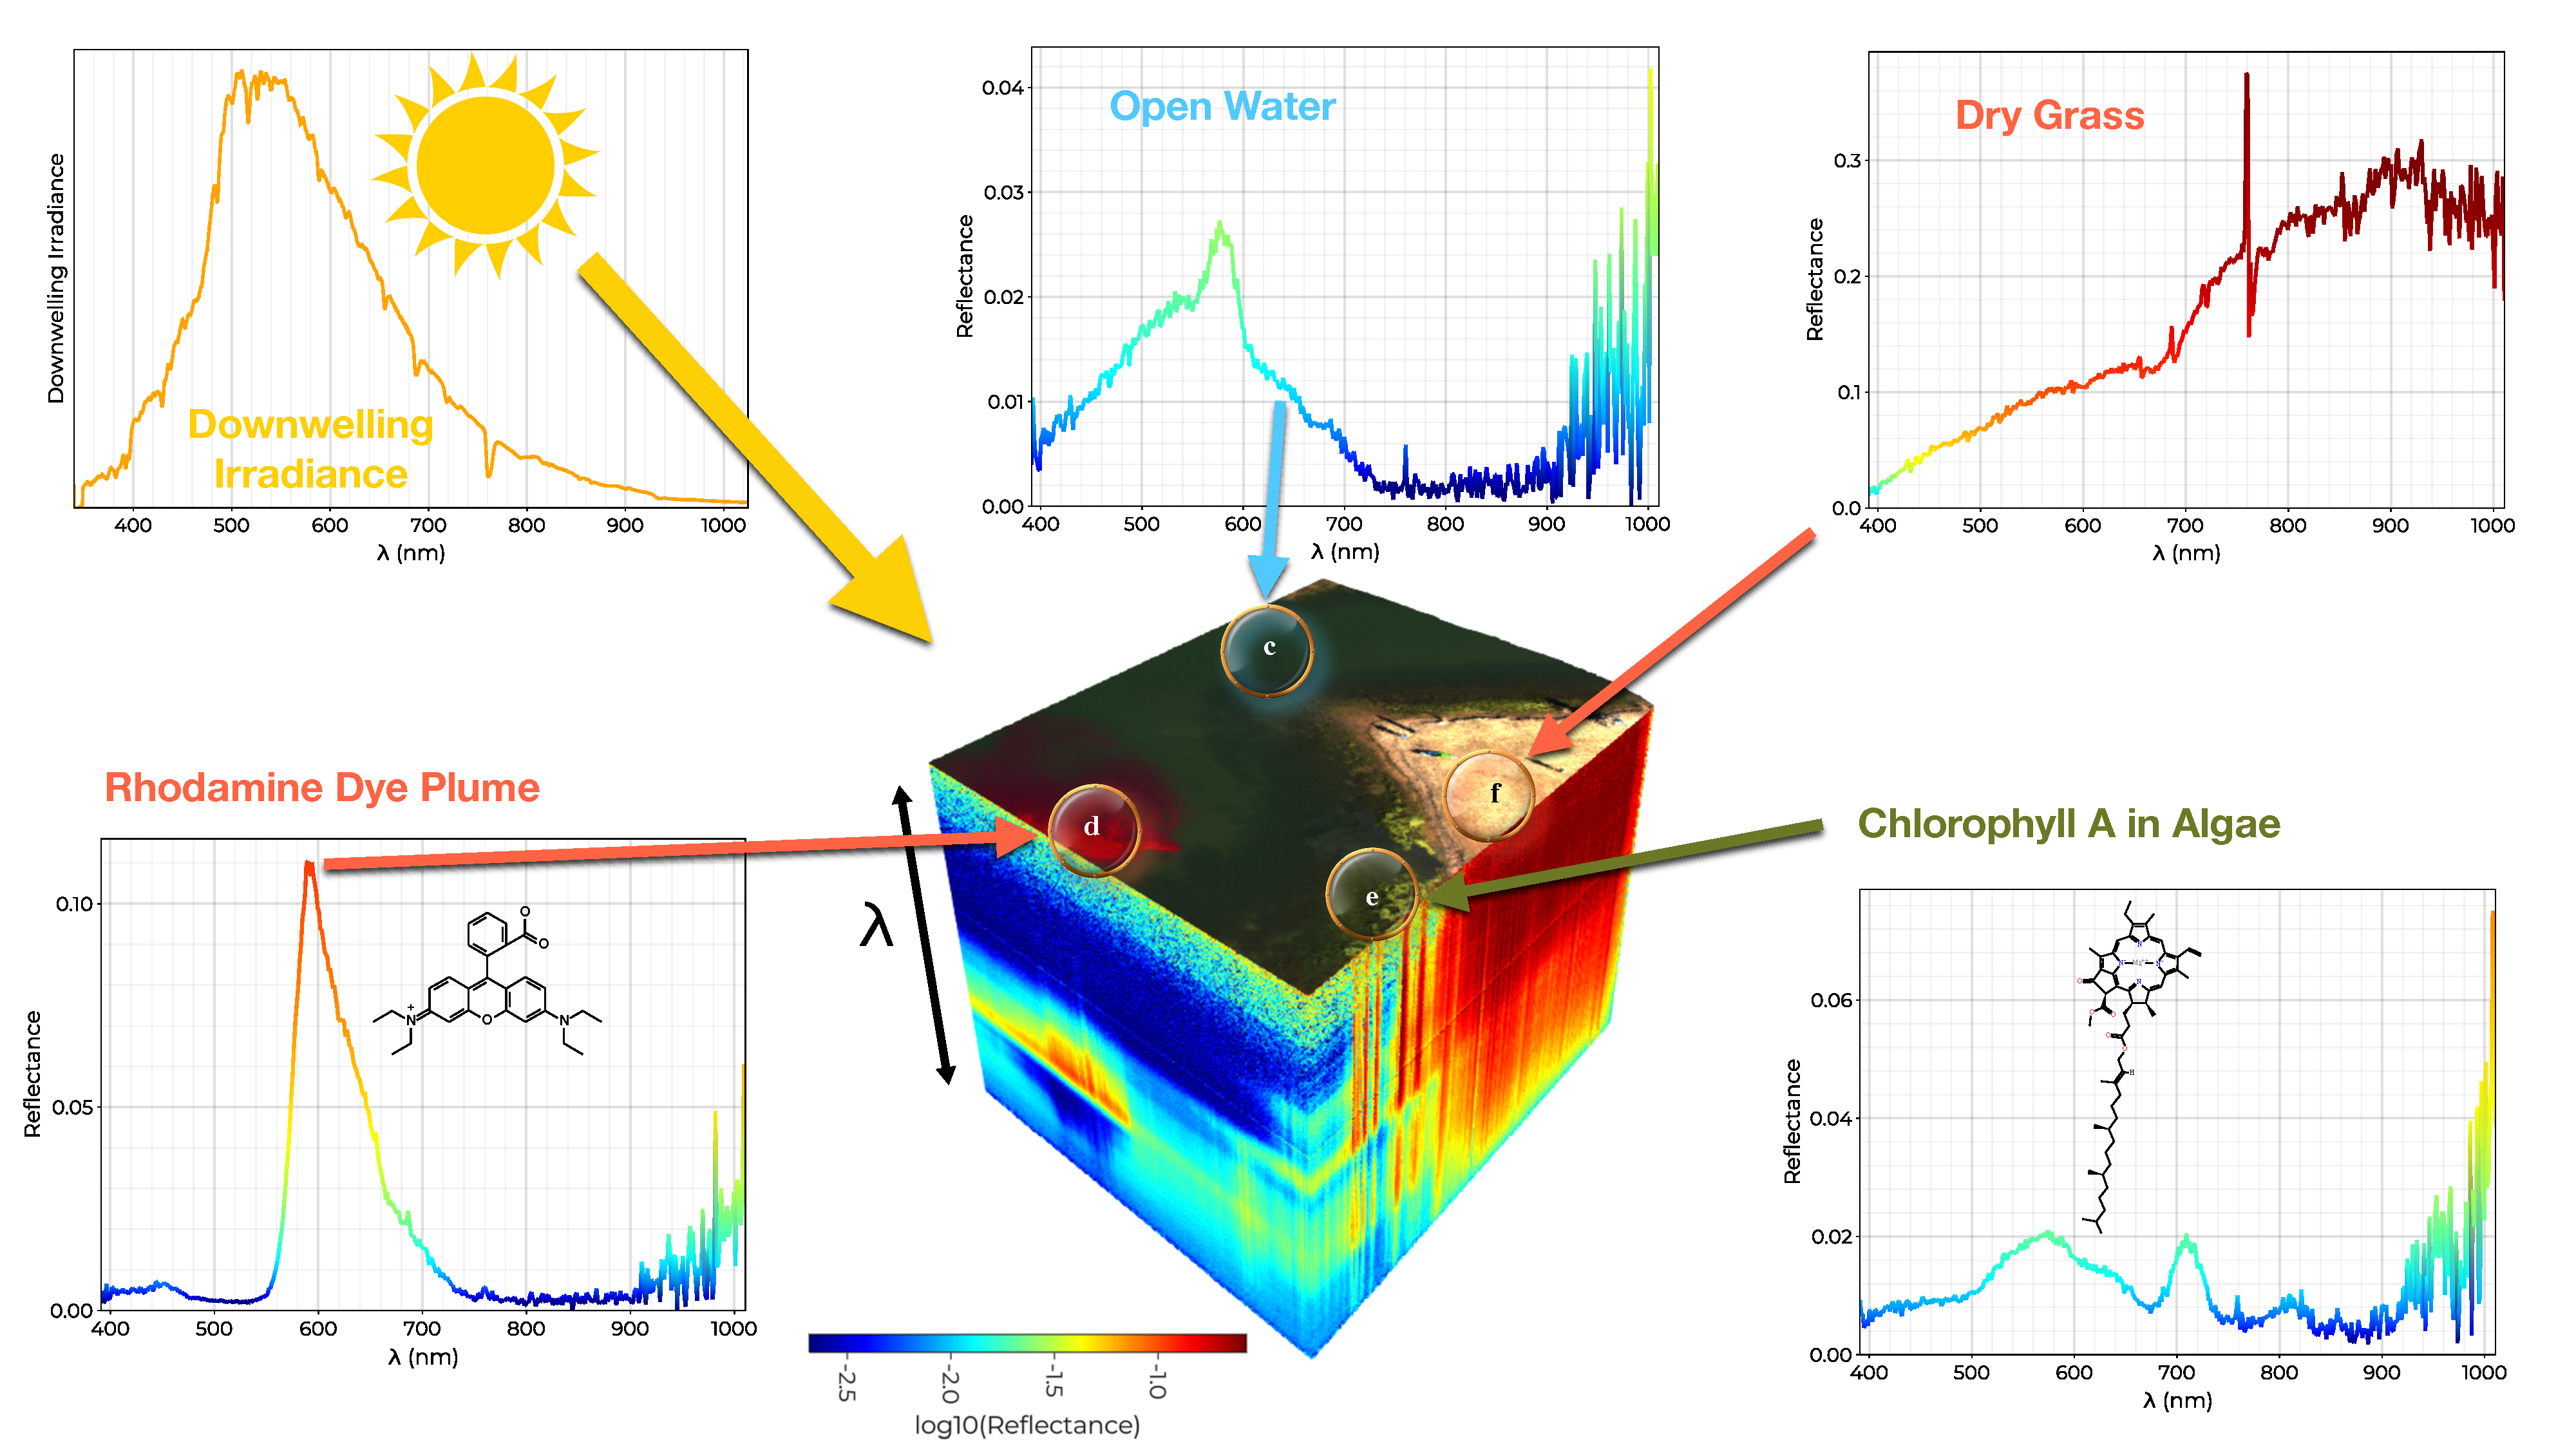
\includegraphics[width=15.5cm]{robot-team-supervised/materials-and-methods/HyperSpectralInfoGraphic.pdf}
\caption{A georectified reflectance data cube is visualized (center) with the $\log_{10}$ reflectance along the z-axis and a pseudo-color image on the top. In the top left, we visualize the downwelling irradiance spectrum (the incident light). The surrounding plots showcase exemplar pixel reflectance spectra for open water, dry grass, algae, and a rhodamine dye plume used to test the system.\label{fig:hsi-infographic}}
\end{figure}  

The above processing workflow was implemented using the Julia programming language: a just-in-time compiled language with native multi-threading support \cite{bezanson2012julia}. By running this pipeline on the onboard computer, we are able to process the collected hyperspectral data cubes in near real time. This feature is critical for time-sensitive applications wherein we need to quickly assess if an area is safe and cannot afford to wait to download and post-process collected imagery after a flight.

\subsection{Data Collection}

The robot team was deployed at a private pond in Montague, Texas, close to the Oklahoma border for three separate collections on 23 November 2020, 9 December 2020, and 10 December 2020. The pond spans an area $<$0.1 km$^{2}$ and has a maximum depth of 3 m. As shown in Figure~\ref{fig:study-area}, the area includes multiple distinct regions with significant small-scale variability. For each acquisition, the UAV first completed a broad survey of the pond, capturing multiple hyperspectral data cubes. Subsequently, the USV sampled across the pond, collecting in situ reference measurements. Each of these reference measurements was then collocated with individual pixel spectra, whereby the USV track overlapped with the UAV's pixels. To account for any time lag in the values measured by the in situ instruments and to account for the USV's size in comparison to the data cube's spatial resolution, each in situ measurement is associated with a 3 $\times$ 3 grid of HSI pixels: that is, a \mbox{30 cm $\times$ 30 cm} square. These combined data form the tabular dataset on which we train regression models; pixel spectra form input features, and each separate USV sensor forms a distinct target variable.

\begin{figure}[H]
\centering
\vspace{-0.1in}
\hspace{-9pt}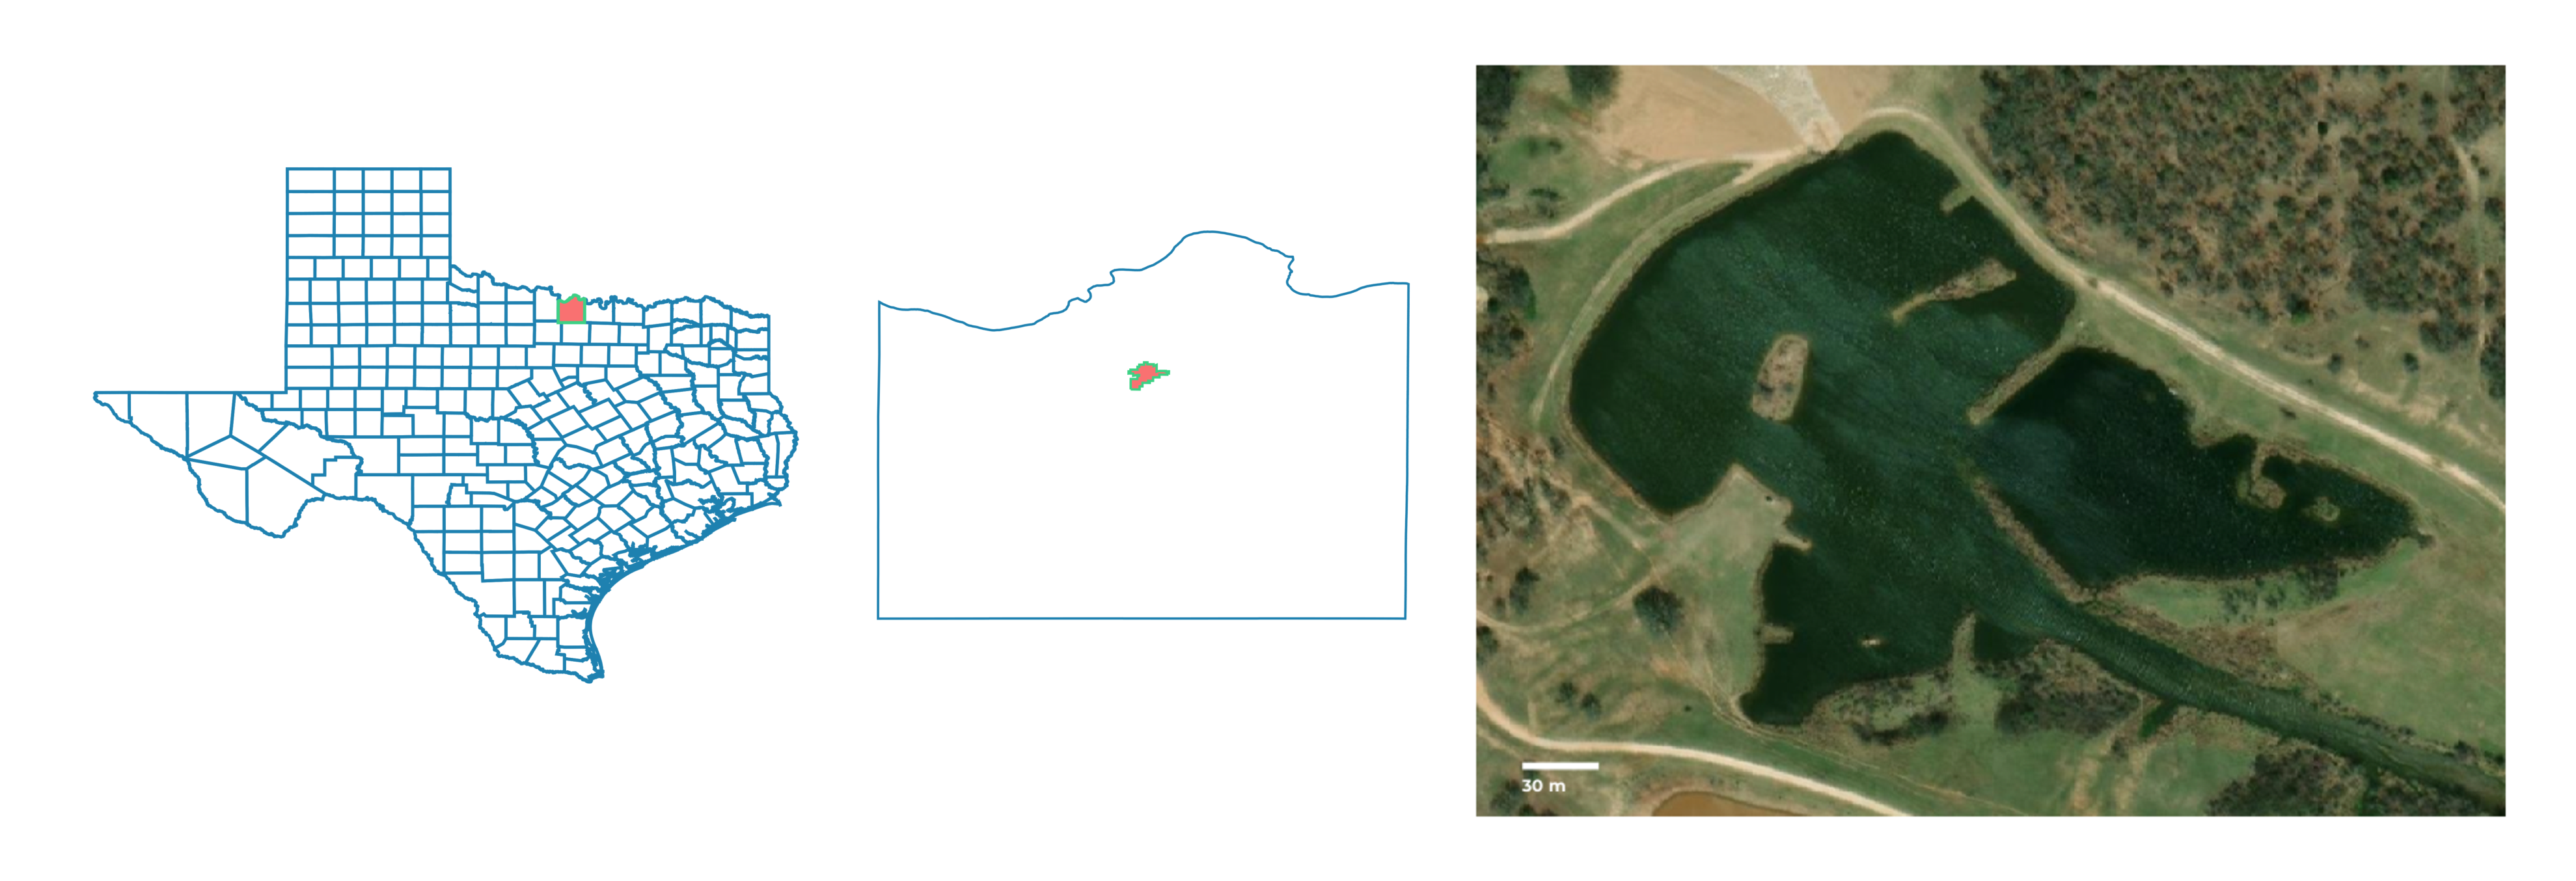
\includegraphics[width=\columnwidth]{robot-team-supervised/materials-and-methods/study-area.pdf}
\vspace{-0.1in}
\caption{The pond in Montague, Texas, where the robot team was deployed. The pond includes multiple distinct regions separated by small islands and grasses. \label{fig:study-area}}
\end{figure}  



Each collection was performed near solar noon to maximize the amount of incident sunlight illuminating the water. For the site in northern Texas, this corresponded to average solar zenith angles of 54.9$^{\circ}$, 56.7$^{\circ}$, and 56.75$^{\circ}$ for 23 November 2020, 9 December 2020, and 10 December 2020, respectively. Given the hyperspectral imager acquires data cubes at nadir, there was little concern for effects due to sunglint. However, to account for any potential variation in lighting conditions between data cubes, we augment the training set with additional features including the drone's viewing geometry (roll, pitch, and heading) and solar illumination geometry (solar azimuth, solar elevation, and solar zenith) as well as the total at-pixel intensity before reflectance conversion, the total downwelling intensity, and the drone's altitude. Further feature engineering is performed to add additional spectral indices that utilize combinations of specific wavelength bands such as the normalized difference vegetation index (NDVI), normalized difference water index (NDWI), simple ratio (SR), photochemical reflectance index (PRI), and more, as outlined in \cite{envi_vegetation_indices, thenkabail2018hyperspectral,kaufman1992atmospherically, SpectralIndexWheat}. A comprehensive list of these added features is provided in Supplementary Table S1. The final dataset includes a total of 526 features (462 reflectance bands plus 64 additional features) with over 120,000 records. 

\subsection{Machine Learning Methods}

For each of the 13 target variables listed in Table~\ref{tab:sensors}, the data were randomly partitioned into a 90:10 training/testing split. To model the data, we chose to use the random forest regressor (RFR) as implemented in the Machine Learning framework for Julia (MLJ) \cite{random-forest-regression, blaom2020mlj}.  Random forests are an ensembling technique based on bagged predictions of individual decision tree regressors trained using the classification and regression trees (CART) algorithm. Each tree in an RFR is trained on a random subset of features and a random subset of training records \cite{decision-trees, random-forest}. Random forests are particularly attractive due to their fast training and inference times. Furthermore, studies continue to observe that tree-based models like random forest remain superior for tabular datasets \cite{grinsztajn2022tree, shwartz2022tabular}.

As reflectance values in adjacent wavelength bins tend to correlate with each other and, therefore, may not necessarily contribute additional information content to the final model, it is desirable to evaluate the relative importance of each feature to the trained model predictions. This is useful both for identifying the most relevant features and for performing feature selection to reduce the final model size. By default, tree-based methods such as RFR allow for impurity-based ranking as described in \cite{random-forest, rfr-importance-ranking}. However, these methods have been shown to be biased towards high cardinality and correlated features \cite{strobl2008conditional}. Therefore, we choose to use the model-agnostic permutation importance as described by \cite{parr2018beware}. To do this, we further partition the training dataset, resulting in an 80:10:10 split with 80\% of the points used for model training, 10\% of the points used for validation and determination of feature importance, and the final 10\% held out as an independent testing set. The importance of the $j^{\text{th}}$ feature is then computed as
\begin{equation}
    \text{Imp}_j = R^2(f(X_{\text{val}}), y_{\text{val}}) - R^2(f(X_{\text{val}}^{(j)}), y_{\text{val}})
\end{equation}
where $(X_{\text{val}}, y_{\text{val}})$ is the validation set, $f(\cdot)$ is the trained model, $R^2(\cdot, \cdot)$ is the coefficient of determination, and $X_{\text{val}}^{(j)}$ is the validation feature set with the $j^{th}$ column randomly permuted. The permutation importance is therefore understood to be the decrease in model performance when the $j^{th}$ feature is replaced by random values from the validation set.

To assess the uncertainty of the final model's predictions, we employed inductive conformal prediction as described in \cite{conformal-prediction-1, conformal-prediction-2, conformal-prediction-3, conformal-prediction-4}. To do this, we computed a set of nonconformity scores of the trained model on the validation set using an uncertainty heuristic: in this case, the absolute error:
\begin{equation}
    s_i = s(X_i, y_i) = \lvert f(X_i) - y_i \rvert = \lvert \hat{y}_i - y_i \rvert
\end{equation}
where $f(X_i)=\hat{y}_i$ denotes the trained ML model applied to the $i^{th}$ calibration record. These n-many scores are sorted, and the interval half width, $d$, is calculated as the $\frac{\lceil(1-\alpha)(n+1) \rceil}{n}$ quantile of this set in order to achieve coverage of $1-\alpha$ on the calibration set. Prediction intervals for new data are then formed as $f(X)\pm d$. For this study, we chose $\alpha=0.1$ for coverage corresponding to a 90\% confidence interval.

Using these tools, the training procedure for each model was as follows: First, each model was trained using six-fold cross-validation on the full 526-feature training set with default hyperparameter values. Feature importances for the trained model were then computed, and the top 25 features were identified. A second model was then trained using the same six-fold cross-validation scheme with only these 25 most important features together with hyperparameter optimization using a random search over the number of trees and sampling fraction. The number of trees was optimized, as it has a significant impact on both model performance and inference time. The sampling ratio determines the fraction of training records that each individual tree is exposed to during training. Tuning this parameter helps limit overfitting by increasing the diversity of trees in the ensemble. Additionally, we chose to fix the maximum tree depth to 20 to control the final model size such that each trained model can fit in-memory on the onboard UAV processing computer. The remaining hyperparameters were left to their default values in order to constrain the total optimization space. The performance of each model was evaluated by computing out-of-fold scores for the coefficient of determination as well as the
\begin{align}
    \text{RMSE} &= \sqrt{\frac{\sum\limits_{i=1}^N (\hat{y}_i-y_i)^2}{N}}, \\
    \text{MAE} &= \frac{\sum\limits_{i=1}^N \lvert \hat{y}_i - y_i \vert}{N},
\end{align}
where RMSE is the root-mean-square error, and MAE is the mean absolute error between the true measurements $y_i$ and the predictions $\hat{y}_i$.

Having identified the model with the best out-of-fold performance, we proceeded to train the final hyperparameter-optimized model on the full training set with the associated uncertainty estimated using conformal prediction.  Then, each final model was evaluated on the previously untouched testing set. We visualize model performance across the distribution of the testing data with a scatter diagram and a quantile--quantile plot, for which successful model predictions should lie close to a 1:1 line.

These trained models can then easily be deployed on the onboard processing computer so that during subsequent surveys, target concentrations can be inferred as imagery are collected and processed. The application of each model to the collected hyperspectral data cubes results in a map of the distribution of the water composition across the pond.




\section{Results}


The final dataset of combined observations from each of the three separate collections contains more than 120,000 individual records. Based on the size of the UAV payload and the available battery capacity, the collection on 23 November 2020 was chosen to cover the broadest possible area, resulting in small horizontal gaps between flight tracks. The collections on 9 December 2020 and 10 December 2020 were designed to complement this collection by sampling a smaller spatial extent with uniform coverage.

The variability of incident lighting conditions for each collection is visualized in Figure~\ref{fig:downwelling-hist}, wherein the distribution of the total downwelling intensity measured by the downwelling irradiance spectrometer across all hyperspectral data cubes is visualized. Despite performing all UAV flights near solar noon, there were differences in the minimum solar zenith angles between collections due to the time of year. Additionally, there was some slight cloudiness during the 9 December and 10 December collections. 

\begin{figure}[H]
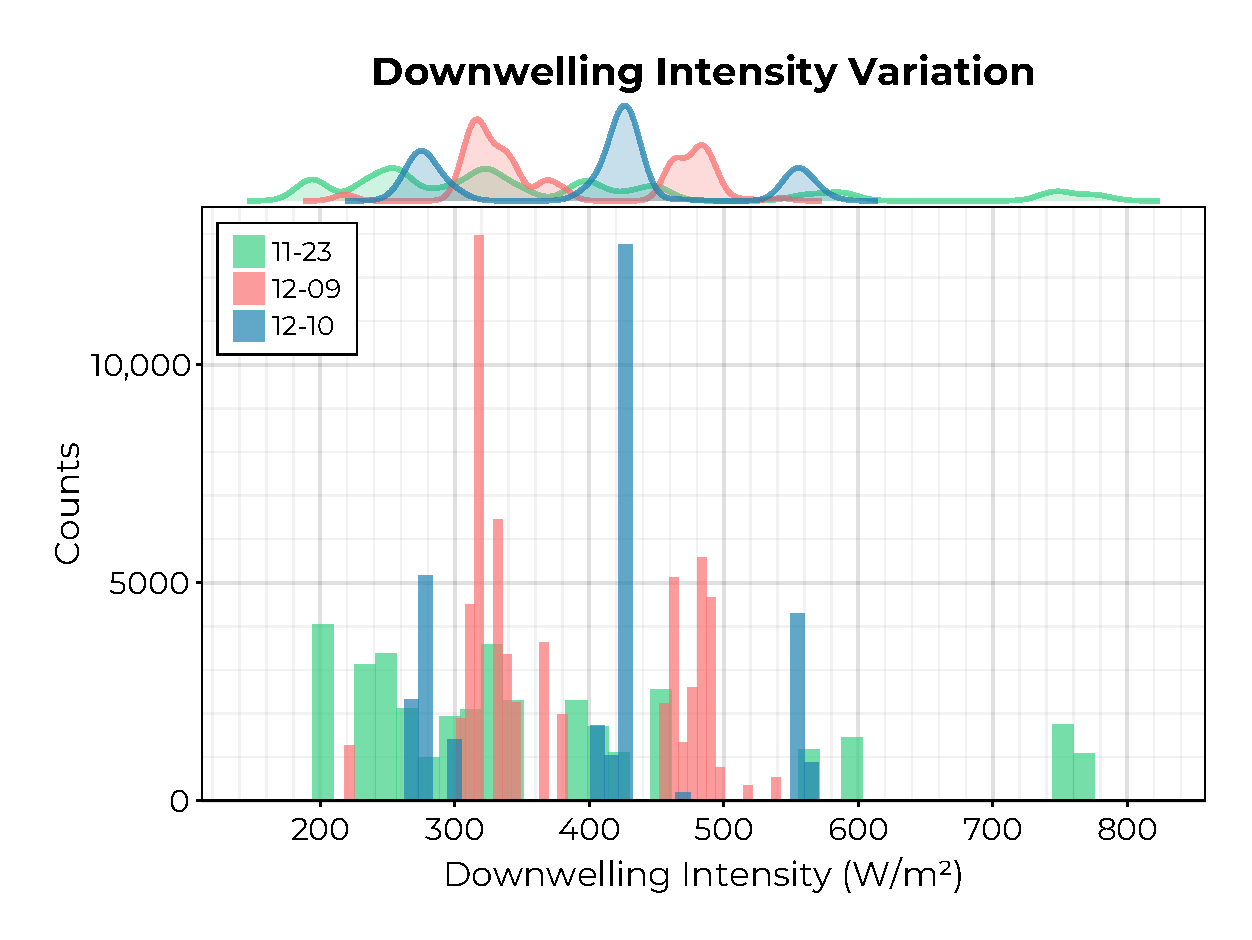
\includegraphics[width=0.7\columnwidth]{robot-team-supervised/results/downwelling-hist.pdf}
\caption{Distribution of total downwelling intensity during each of the three HSI collection flights. The multi-modal nature of these distributions reflects the impact of the relative orientation of the drone to the sun as well as potential occlusion due to the presence of clouds.\label{fig:downwelling-hist}}
\end{figure}   

The results of the model training procedure are presented in Table~\ref{tab:fit-results}. The performance of the model is identified by the $R^2$, RMSE, and MAE out-of-fold estimates (mean $\pm$ standard deviation) of the final hyperparameter-optimized model in the training set, with the target variables ranked in descending order by the $R^2$ value and separated by sensor type (physical variables, ions, biochemical variables, and chemical variables). The final hyperparameter values for each model are listed in Table~\ref{tab:hyperparameters} in Appendix~\ref{Model Hyperparameters}. The small variation in values across folds confirms that the reported performance is independent of how the training set was sampled. Furthermore, we report the interval width that yields a 90\% confidence interval on the holdout validation set determined by the conformal prediction procedure. We then evaluate how the estimated uncertainty generalizes by computing the empirical coverage on the holdout testing set: that is, we compute the percentage of predictions in the test set that actually fall within the estimated 90\% confidence interval. 

From Table~\ref{tab:fit-results},  we see that the empirical coverage achieved by the inferred confidence interval evaluated in the independent test set is within 1\% of our desired coverage for each target modeled. This indicates that the uncertainties obtained by the conformal prediction procedure are reliable---at least within the bounds of the collected dataset. We also note that in all cases, the inferred model uncertainties are larger than the resolution of the in situ sensors. This lends further credence to the inferred uncertainty estimates, as we should not expect to be able to have lower uncertainty than the smallest resolvable difference in reference sensor measurements.

To further examine the differences in model performance between the target variables, we can consider the difference between the RMSE and MAE scores. The MAE is less sensitive to the impact of outliers than the RMSE, and as a consequence, any large difference between the two is indicative of impacts due to the distribution of target values. Indeed, this is the case for turbidity, for which almost all measurements were below 10 FNU, with only a small fraction of observations from a small area near the shore being above this value. %Please ensure meaning has been retained. 
The rest of the models all show mean per-fold RMSE values with sizes comparable to the mean per-fold MAEs. 

In the remainder of this section, we compare the models within each target category.

% \pagebreak

\begin{sidewaystable}[p!]
  \caption{Summary of fitting statistics for each target measurement. Models
    were evaluated using 6-fold cross-validation on the training set. The
    estimated uncertainty is evaluated so that a prediction $\hat{y}\pm \Delta
    y$ achieves 90\% coverage on the calibration holdout set. The empirical
    coverage is the percentage of predictions in the testing set that fall
    within the inferred confidence interval.}
  \label{tab:fit-results}
  \begin{center}
    \resizebox{\textwidth}{!}{\begin{tabular}{lcccccc} \hline
      & & & & & & \\
      %\textbf{Target} & \textbf{Units} & \textbf{$\text{R}^2$} & \textbf{RMSE} & \textbf{MAE} & \textbf{Estimated Uncertainty} & \textbf{Empirical Coverage (\%)} \\
      \textbf{Target} & \textbf{Units} & \textbf{$\text{R}^2$} & \textbf{RMSE} & \textbf{MAE} & \textbf{Estimated} & \textbf{Empirical} \\
      & & & & & \textbf{Uncertainty} & \textbf{Coverage (\%)}\\ \hline
      Temperature & $^{\circ}$C & 1.0 ± 6.04 $\times$ 10$^{-6}$ & 0.0289 ± 0.000466 & 0.0162 ± 0.00016 &  ±0.039 & 90.3 \\
      Conductivity & $\mu$S/cm & 1.0 ± 1.54 $\times$ 10$^{-5}$ & 0.574 ± 0.0128 & 0.322 ± 0.00579 &  ±0.76 & 90.6 \\
      pH & 0--14 & 0.994 ± 0.000288 & 0.0145 ± 0.000304 & 0.00739 ± 9.49 $\times$ 10$^{-5}$ &  ±0.017 & 89.5 \\
      Turbidity & FNU & 0.897 ± 0.00611 & 3.13 ± 0.084 & 0.736 ± 0.0156 &  ±1.1 & 89.8 \\
      \hline
      $\mathrm{Ca}^{2+}$ & mg/L & 1.0 ± 1.06 $\times$ 10$^{-5}$ & 0.285 ± 0.00357 & 0.137 ± 0.00224 &  ±0.33 & 89.8 \\
      $\mathrm{Cl^-}$ & mg/L & 0.995 ± 0.000196 & 0.895 ± 0.0202 & 0.516 ± 0.00759 &  ±1.2 & 90.1 \\
      $\mathrm{Na^+}$ & mg/L &0.993 ± 0.000229 & 6.16 ± 0.102 & 2.83 ± 0.0303 &  ±7.3 & 90.0 \\
      \hline
      Blue--Green Algae (Phycoerythrin) & ppb & 0.995 ± 0.000601 & 0.783 ± 0.0489 & 0.287 ± 0.00959 &  ±0.73 & 89.3 \\
      CDOM & ppb &  0.965 ± 0.00352 & 0.248 ± 0.0142 & 0.0921 ± 0.0024 &  ±0.15 & 89.9 \\
      Chlorophyll-a & ppb & 0.908 ± 0.00664 & 0.37 ± 0.00934 & 0.131 ± 0.00228 &  ±0.27 & 89.2 \\
      Blue--Green Algae (Phycocyanin) & ppb & 0.708 ± 0.00689 & 0.749 ± 0.0129 & 0.446 ± 0.00405 &  ±0.93 & 89.8 \\
      \hline
      Crude Oil & ppb & 0.949 ± 0.00267 & 0.247 ± 0.00597 & 0.0935 ± 0.00114 &  ±0.17 & 89.8 \\
      Optical Brighteners & ppb & 0.943 ± 0.00122 & 0.0806 ± 0.0014 & 0.0481 ± 0.000416 &  ±0.095 & 89.8 \\
    \end{tabular}}
  \end{center}
\end{sidewaystable}

\newpage

\subsection{Physical Variables}

Physical variables included temperature, conductivity, pH, and turbidity. In the combined dataset, the distributions for temperature and conductivity had two distinct, nonoverlapping regions corresponding to the measurements from 23 November and the measurements from 9 December and 10 December, respectively. The pH value of the pond was slightly alkaline, showing a multimodal spatial distribution with values ranging from 8.0 to 8.6. As mentioned above, the pond water was very clear for each observation period, with most turbidity values ranging between 1 and 3 FNU and very few above 10.

The results of the hyperparameter-optimized RFR fits are shown in Figure~\ref{fig:physical-fit}. Temperature and conductivity show the best performance in the independent training set, with $R^2$ values of 1.0 (to three decimal places). Similarly, the pH model achieves an excellent fit, with most predictions falling close to the 1:1 line. Quantile--quantile plots for these three models further confirm that the distributions of the true and predicted values match. The turbidity model also achieves a strong fit, with a $R^2$ value of 0.905. The scatter diagram and quantile--quantile plot for this target show that the model performance degrades with larger values, for which deviation in the predicted distribution is apparent past 25 FNU.

\begin{figure}[H]
  \centering
  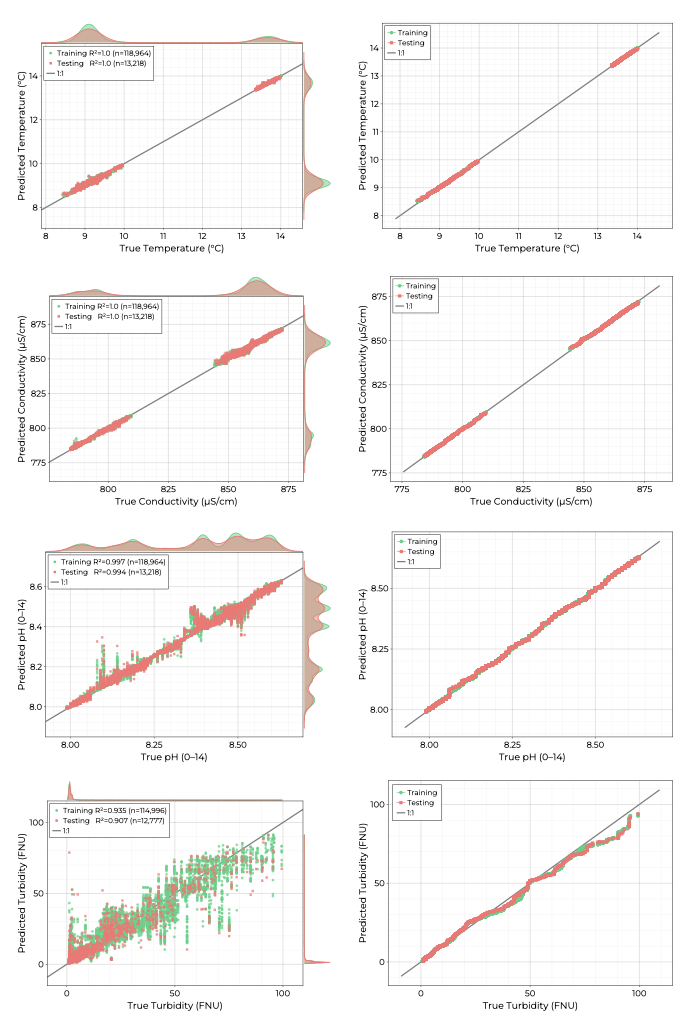
\includegraphics[width=0.8\textwidth]{robot-team-supervised/results/fits/physical-fitres.png}
  \caption{Scatter diagrams (\textbf{left}) and quantile--quantile plots (\textbf{right}) for the hyperparameter-optimized RFR models for the physical variables measured by the USV.\label{fig:physical-fit}}
\end{figure}

The permutation importance of the top 25 features for each of the models of the physical variables is shown in Figure~\ref{fig:physical-fi}. All four models show strong dependence on the solar illumination geometry (solar azimuth, elevation, and solar zenith) as well as the viewing geometry (pitch, altitude, heading, etc.). All four models also include the total downwelling intensity and the total pixel intensity as highly important features. The temperature, conductivity, and pH models all include red-to-infrared reflectance bins and a combination of spectral indices within their most important features. Finally, the turbidity model relies mainly on blue wavelengths from 462 to 496 nm and did not include any spectral indices amongst the 25 most important features.

By applying the trained models to the full hyperspectral data cubes, we can produce maps of the distributions of the target variables as in Figure~\ref{fig:map-physical}. Here, we have chosen to show the map produced from the imagery collected during the 23 November collection period, as it showcases the largest spatial extent. The temperature map shows lower values near the shore, which is to be expected as the air temperature was below the water temperature. The temperature, conductivity, and pH maps all show a distinction between the main body of water and the alcove to the east, which receives little flow from the main body. The turbidity map confirms that the water is largely clear but has elevated levels near the shore.


\begin{figure}[H]
  \centering
  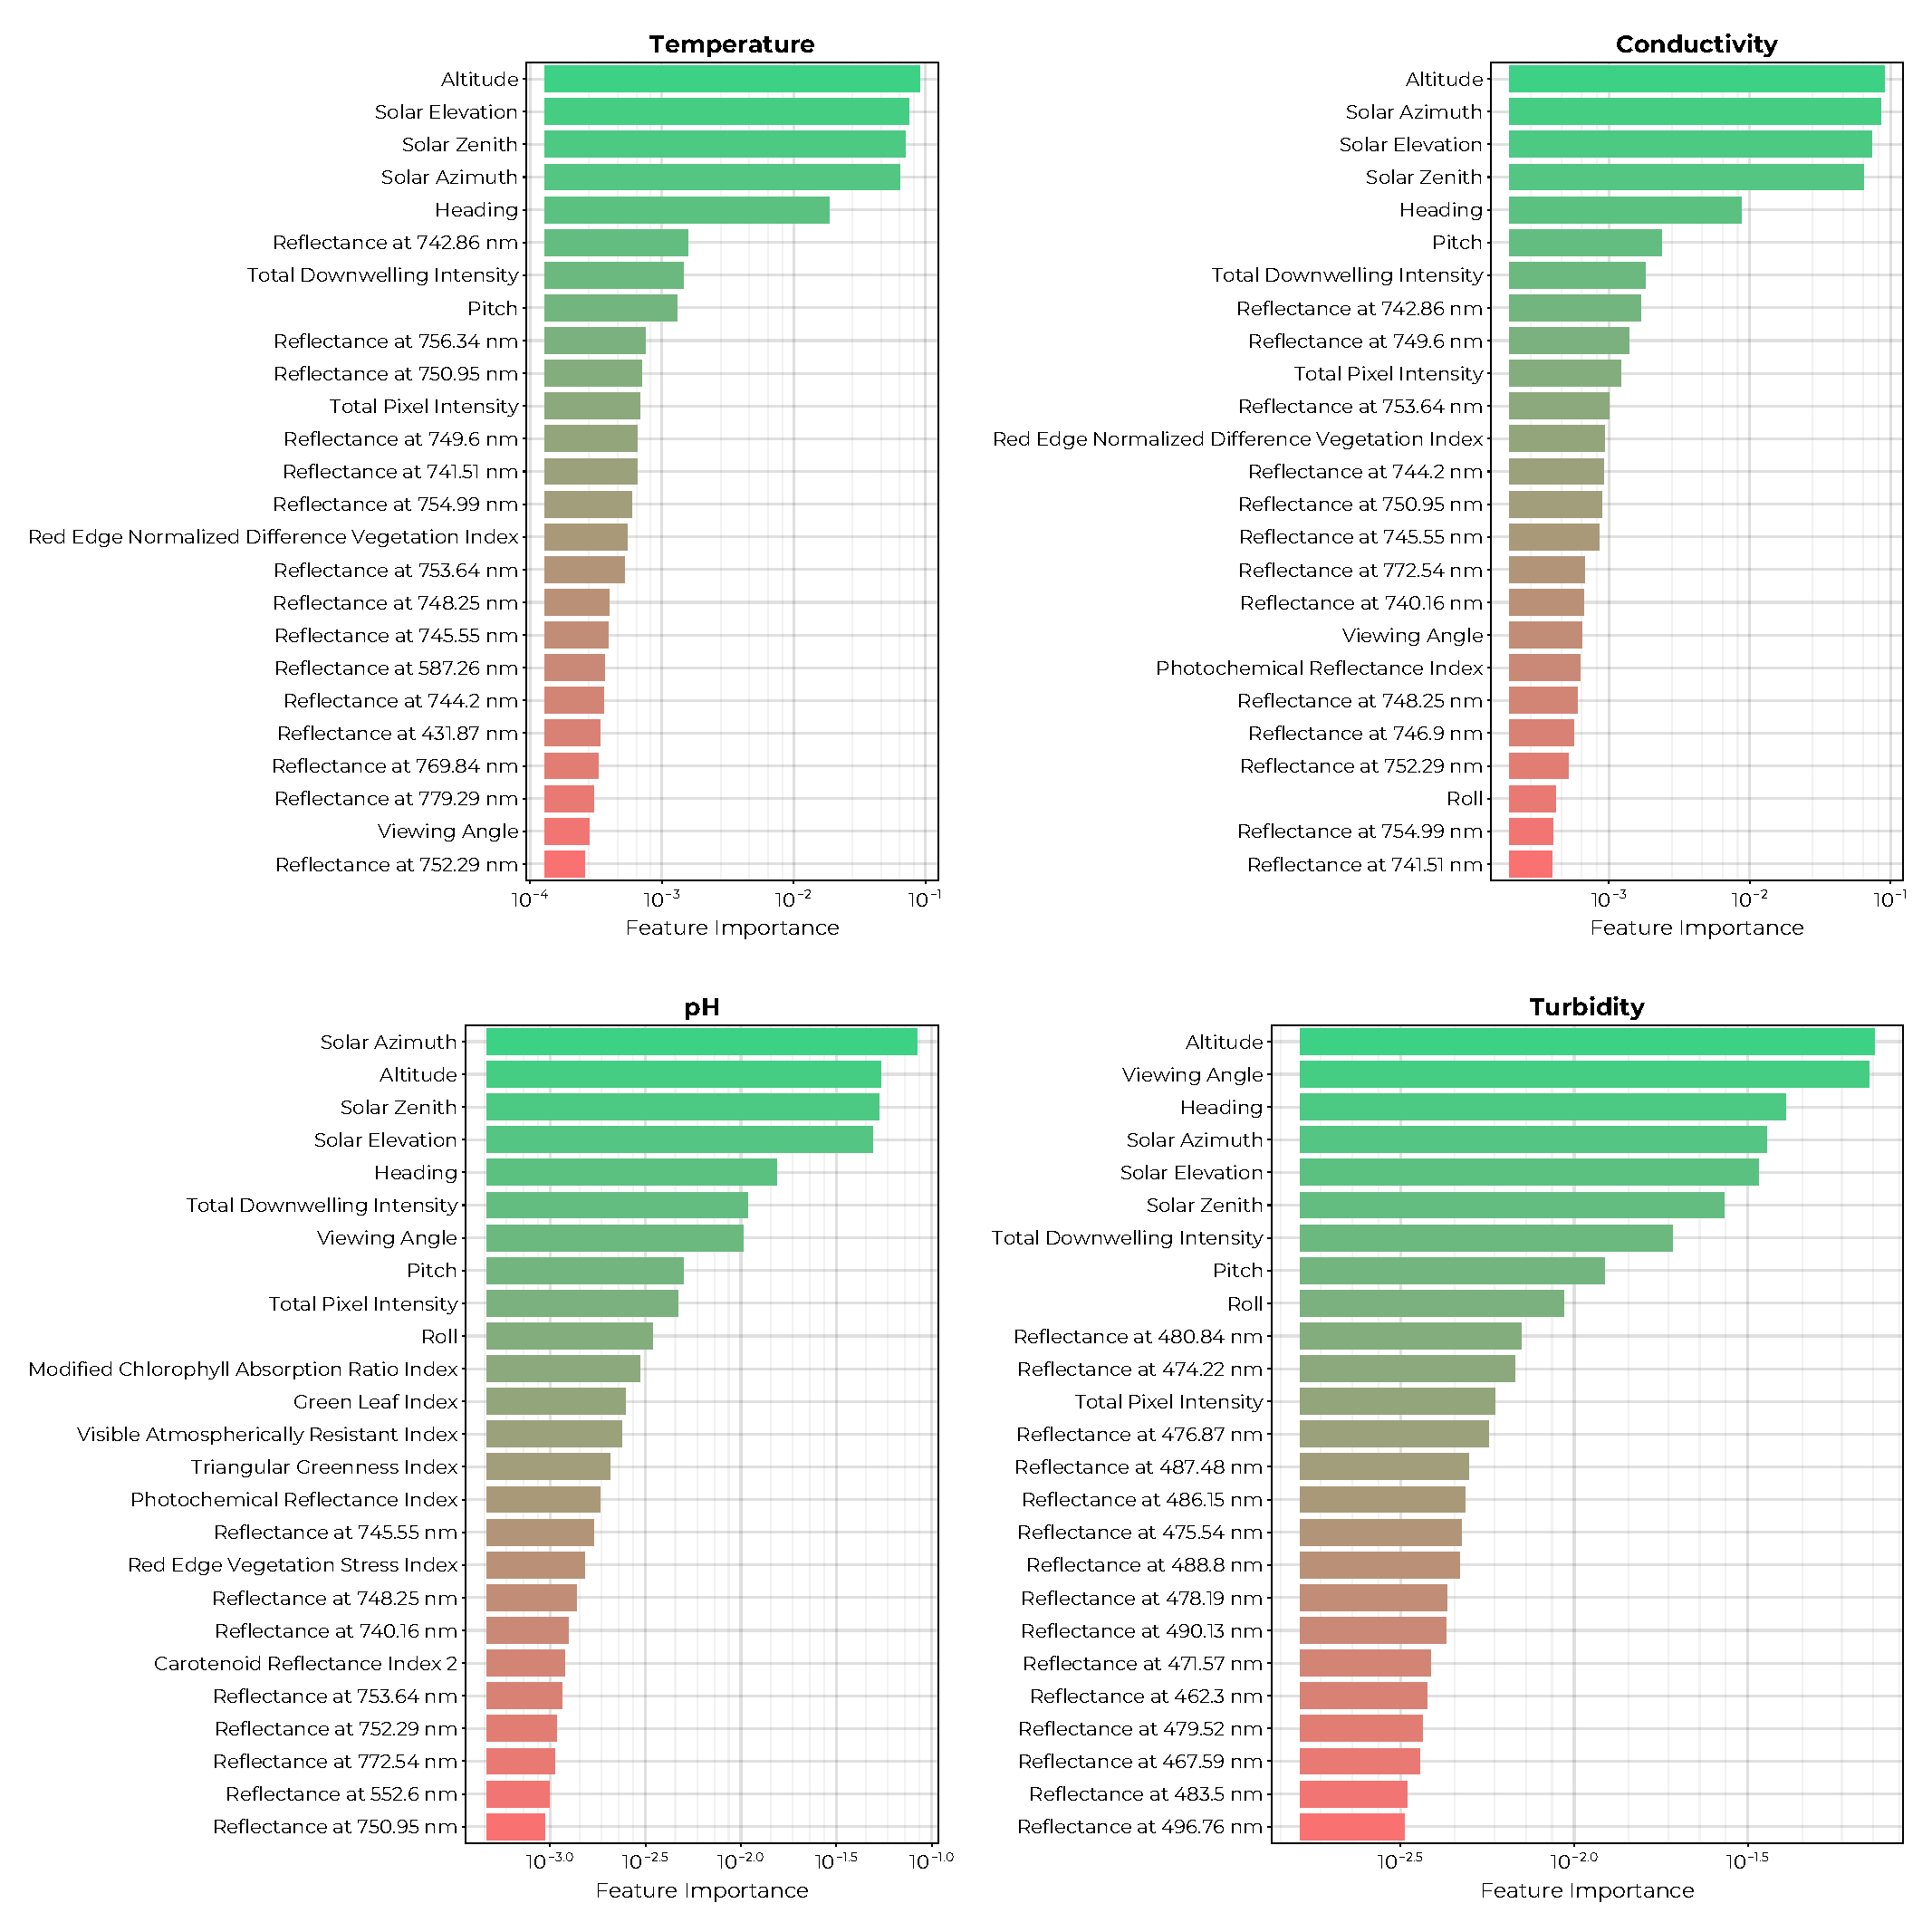
\includegraphics[width=1.0\textwidth]{robot-team-supervised/results/fits/physical-ranking.pdf}
  \caption{Ranked permutation importance for each feature in the physical variable models. Permutation importance measured the decrease in the model's $R^2$ value after replacing each feature in the prediction set with a random permutation of its values.\label{fig:physical-fi}}
\end{figure}


\begin{figure}[H]
  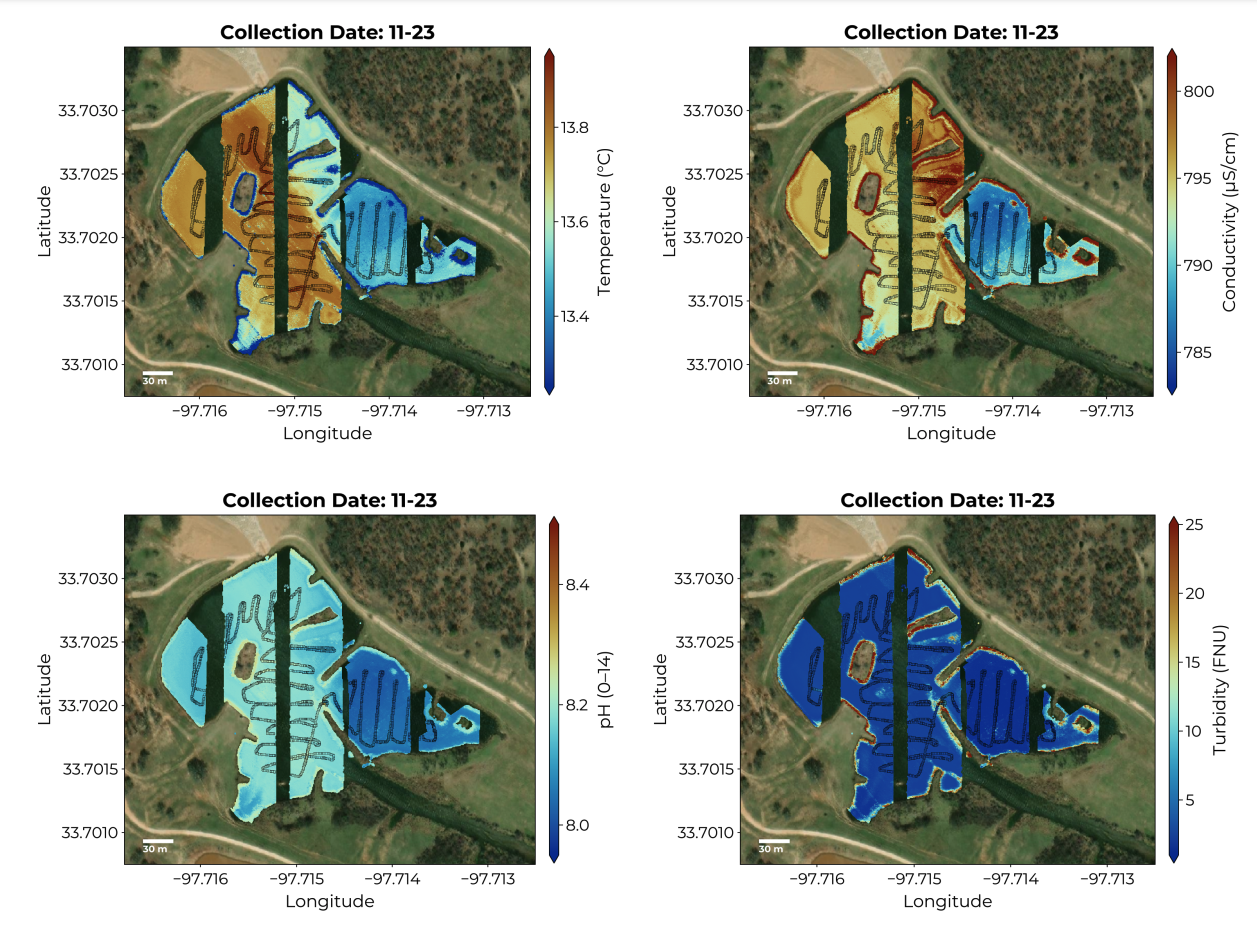
\includegraphics[width=0.9\textwidth]{robot-team-supervised/results/maps/physical.png}
  \caption{Maps generated by applying each of the physical variable models to the hyperspectral data cubes collected on 23 November. Overlaid over the predictions are color-filled squares showing the associated in situ reference data for the same collection period. The size of the squares has been exaggerated for visualization. We note that there is good agreement between the model predictions and the reference data. \label{fig:map-physical}}
\end{figure}



\subsection{Ions}

The measured ions include $\mathrm{Ca}^{2+}$, $\mathrm{Cl}^{-}$, and $\mathrm{Na}^{+}$. All three measurements showed multimodal spatial distributions throughout the pond on each of the three collections. The scatter diagrams and quantile--quantile graphs for the resulting fits are shown in Figure~\ref{fig:ions-fit}. All three models achieved excellent fits, with $R^2$ values of 1.0, 0.996, and 0.993 on the independent testing set, respectively. Furthermore, there is no clear decrease in model performance for low or high concentrations; rather, for $\textrm{Cl}^{-}$ and $\textrm{Na}^{+}$, the models have the most difficulty in the middle of the target distributions. 

The permutation importance rankings for the top 25 features of each of the ion models is shown in Figure~\ref{fig:ions-fi}. Here, we see that all three models depend on the solar illumination and viewing geometries as well as the total downwelling intensity and the total pixel intensity measured by the hyperspectral imager. All three models utilize a combination of spectral indices that combine green, red, and infrared reflectance bins. The $\textrm{Ca}^{+}$ and $\textrm{Cl}^{-}$ models depend on specific red wavelengths of 740 to 769 nm. $\textrm{Cl}^{-}$ and $\textrm{Na}^{+}$ also depend on green and yellow reflectance bins of 541 to 589 nanometers.

The maps produced by applying the fitted models to the hyperspectral data cubes for 23 November are shown in Figure~\ref{fig:map-ions}. Both positive ions $\mathrm{Ca}^{2+}$ and $\mathrm{Na}^{+}$ show high concentrations in the northwest portion of the pond, with lower values being measured in the alcove on the eastern side. Positive ion concentrations also appear to decrease near the shore. The negative ion $\mathrm{Cl}^{-}$ shows the opposite distribution, with larger values in the alcove to the east and the lowest values on the western side of the pond. The $\mathrm{Cl}^{-}$ ion concentration also appears to increase near the shore.

\begin{figure}[H]
  \centering
  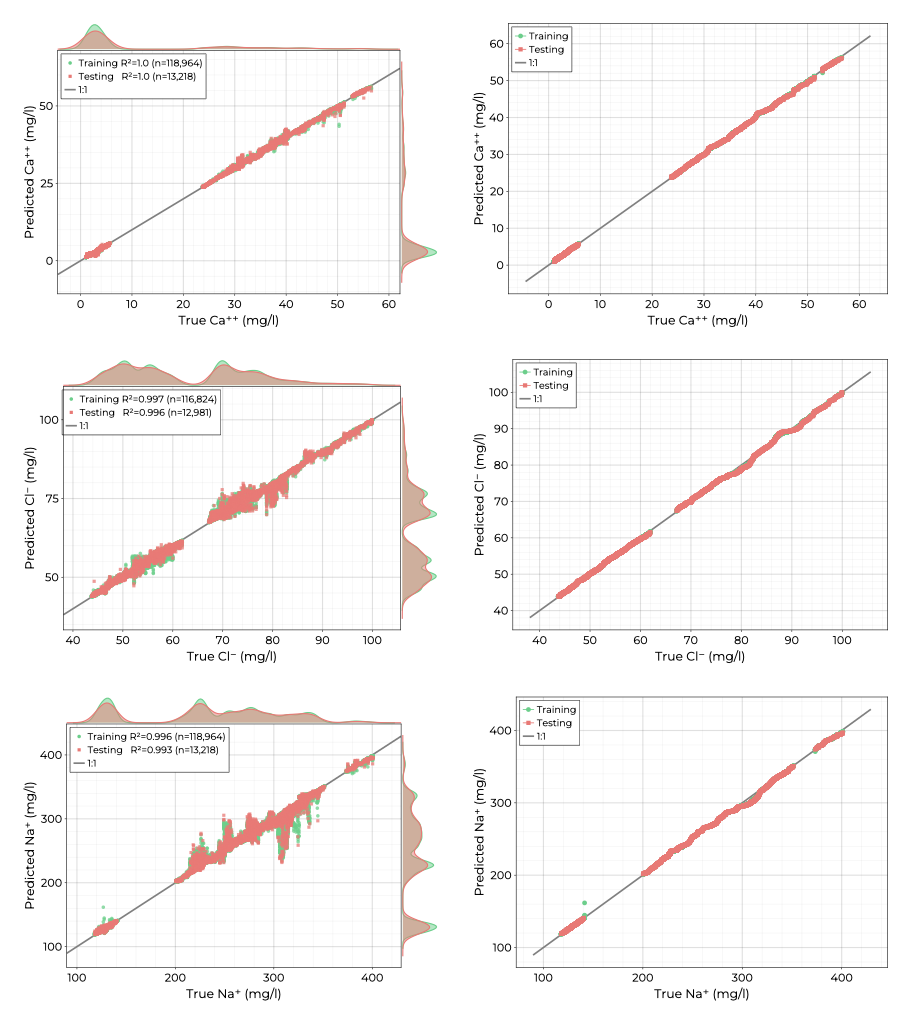
\includegraphics[width=\columnwidth]{robot-team-supervised/results/fits/ions-fitres.png}
  \caption{Scatter diagrams (\textbf{left}) and quantile--quantile plots
    (\textbf{right}) for the hyperparameter-optimized RFR models for the ion
    measurements made by the USV.\label{fig:ions-fit}}
\end{figure}

\begin{figure}[H]
  \centering
  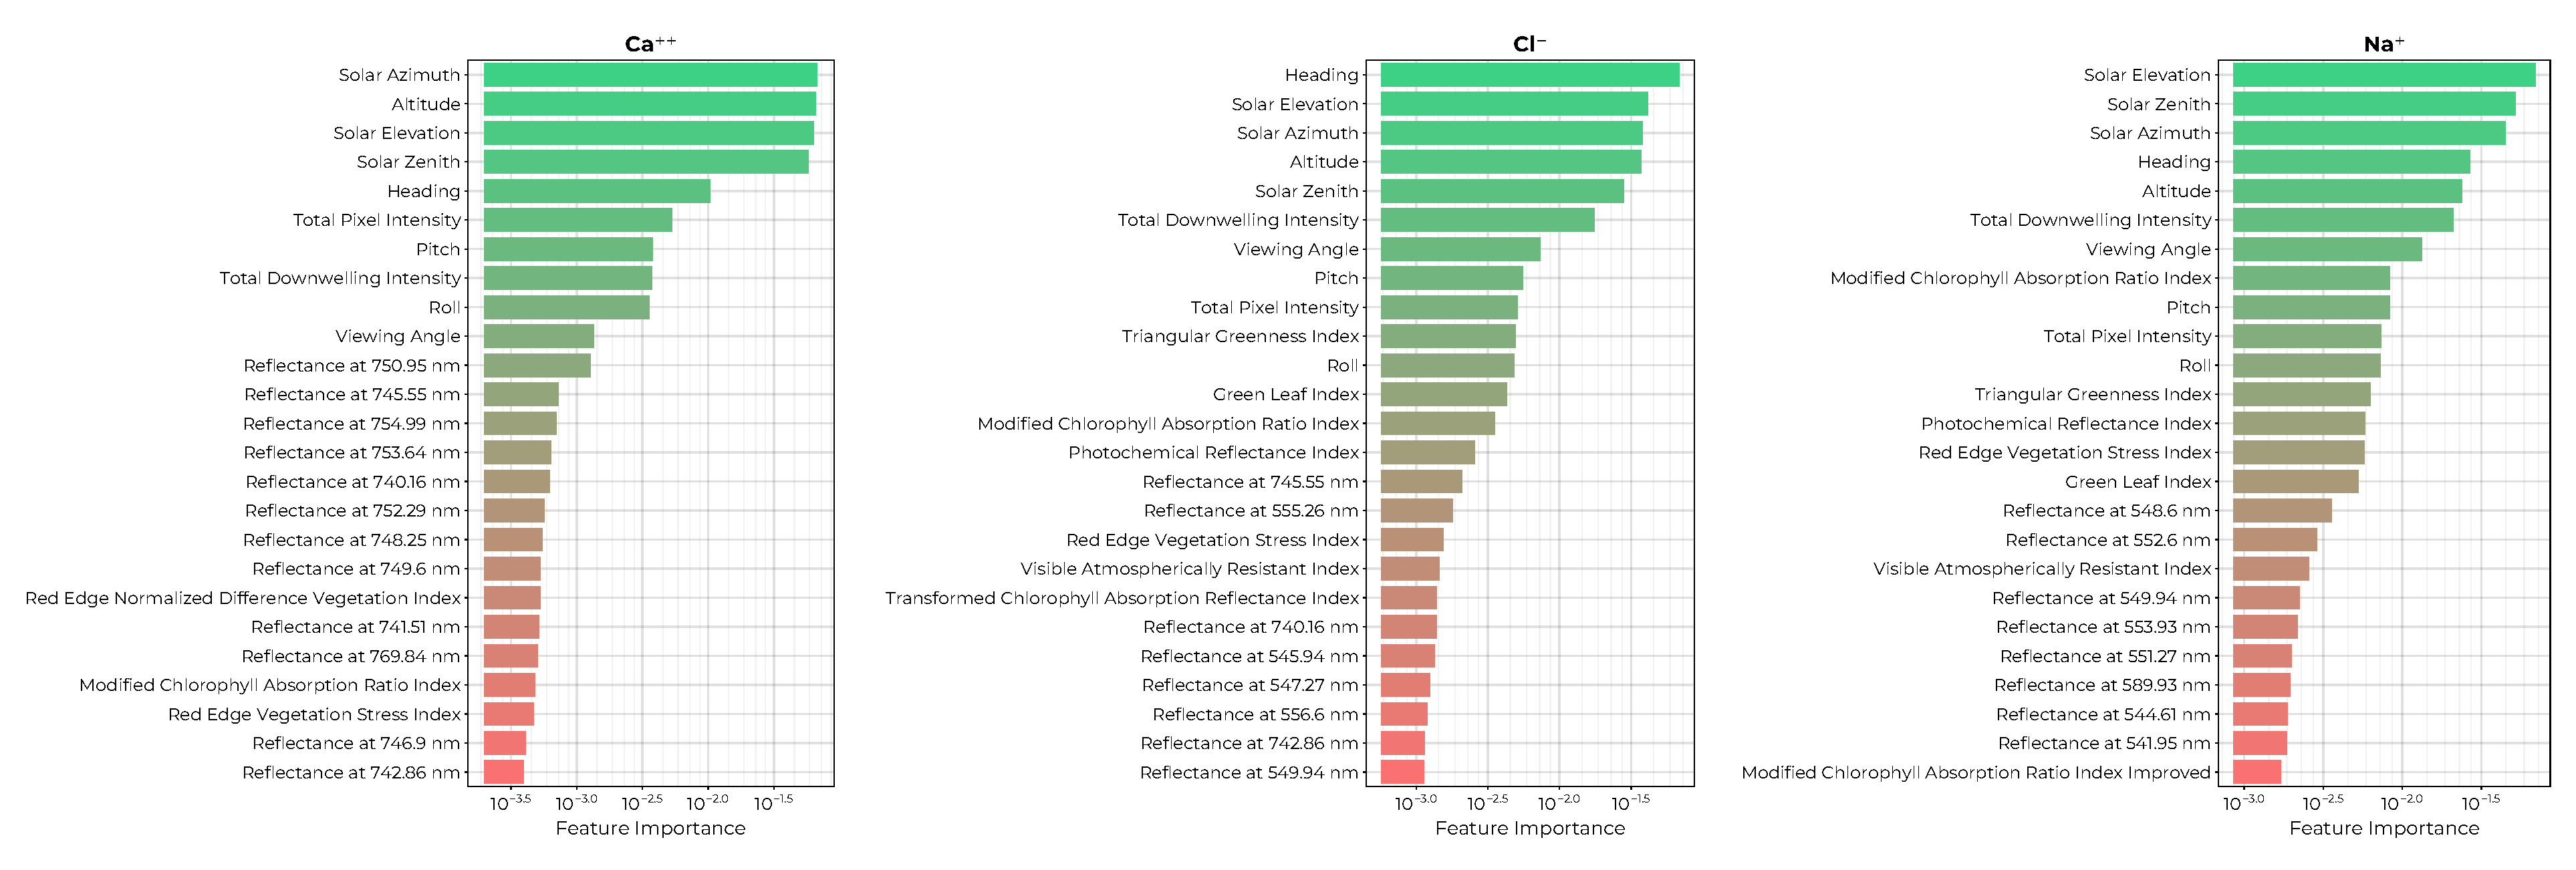
\includegraphics[width=0.9\columnwidth]{robot-team-supervised/results/fits/ions-ranking.pdf}
  \caption{Ranked permutation importance for the top 25 features of the ion
    models. The permutation importance measures the decrease in the model's
    $R^2$ value when each feature is replaced by a random permutation of its
    values.\label{fig:ions-fi}}
\end{figure}  

\begin{figure}[H]
  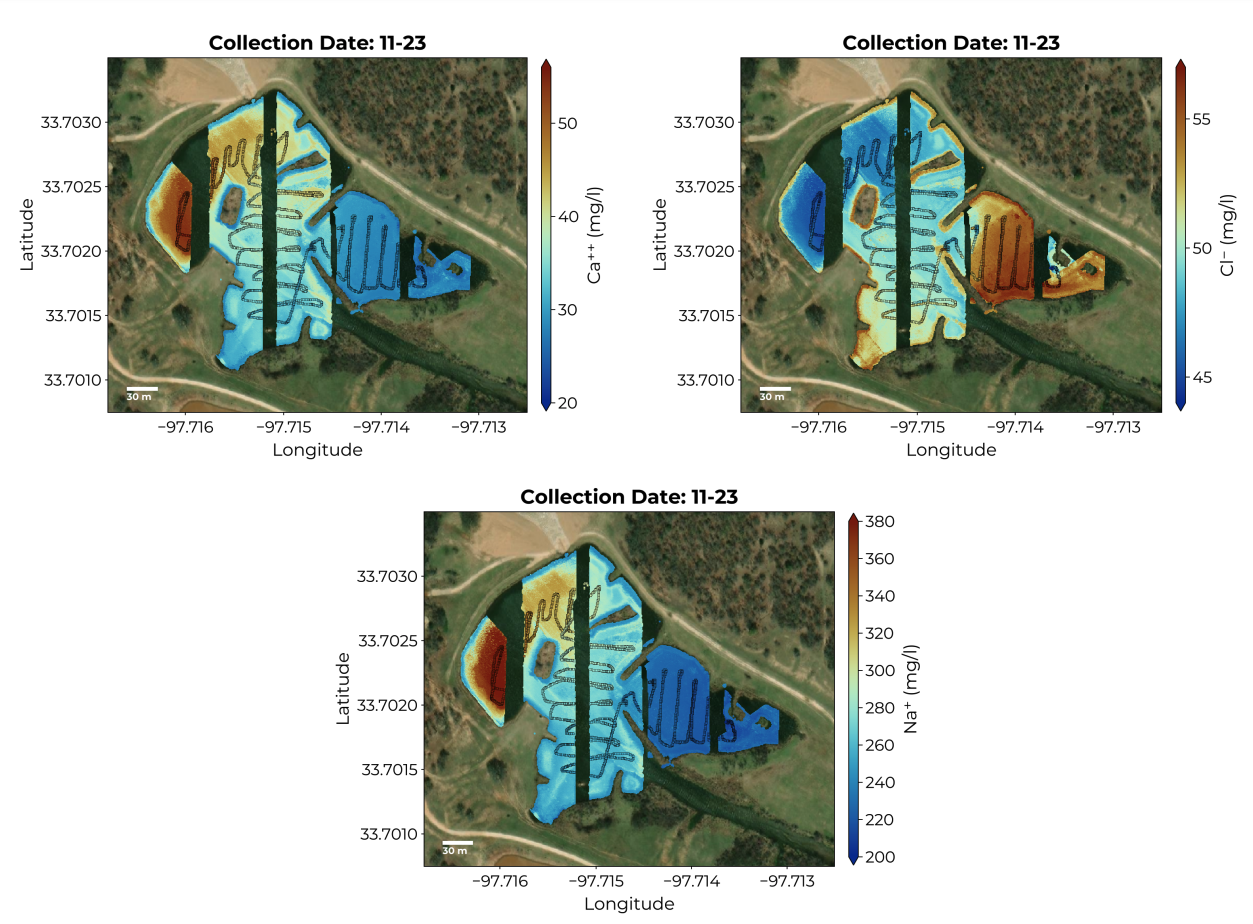
\includegraphics[width=\columnwidth]{robot-team-supervised/results/maps/ions.png}
  \caption{Maps generated by applying the trained ion models to the data cubes collected on 23 November. Overlaid on the maps are the in situ reference measurements for the same collection period. The size of the squares has been exaggerated for the visualization. We note that there is good agreement between the generated map and the reference data. \label{fig:map-ions}}
\end{figure}  



\subsection{Biochemical Variables}

The measured biochemical variables include the pigments phycoerythrin, phycocyanin, and chlorophyll-a, as well as CDOM. Phycoerythrin and phycocyanin are both present in blue--green algae, and chlorophyll-a is found in all photosynthetic organisms except bacteria. In the combined dataset, the three pigments showed multimodal distributions separated by the collection day and with little spatial variation within each individual collection. CDOM showed a variable spatial distribution throughout the pond between the main water body and the eastern alcove on 23 November.

The results of the RFR fits for the biochemical variables are shown in Figure~\ref{fig:biochem-fit}. Phycoerythrin showed the best model performance, with an $R^2$ value of 0.995 in the training set. Both CDOM and chlorophyll-a achieved good performance, with $R^2$ values of 0.967 and 0.917 in the training set. Quantile--quantile plots indicate that the CDOM model degrades for values below 16 ppb, where data are sparse. The chlorophyll-a model shows the opposite trend, with poorer performance for concentrations above 5 ppb, for which there are very few records. The phycocyanin model had the lowest performance of the biochemical sensors, with an $R^2$ value of 0.727 and with model predictions rapidly decreasing in quality for concentrations greater than 3 ppb. 

The permutation importance ranking of the top 25 features of each biochemical model is shown in Figure~\ref{fig:biochem-fi}. Again, all four models include the solar illumination and viewing geometries amongst their most important features as well as the total downwelling intensity and total pixel intensity at the imager. Additionally, all four models include some vegetation indices amongst the top features, which utilize combinations of blue, green, yellow, red, and infrared reflectance bands. The phycoerythrin model shows a preference for green reflectance bins from 544 to 556 nm, while the phycocyanin model prefers blue and red reflectance bins. The CDOM model uses mainly red reflectance values, whereas the chlorophyll-a model includes red, green, and blue reflectance bins.

The maps generated for the 23 November collection by applying trained biochemical models are shown in Figure~\ref{fig:map-biochem}. The three pigments show low concentrations in the body of water but elevated levels near the shore. The CDOM distribution shows spatial variability, with higher values in the eastern alcove---similar to the separation seen in the maps for temperature, conductivity, $\textrm{Ca}^{2+}$, $\textrm{Cl}^{-}$, and $\textrm{Na}^{+}$.

\begin{figure}[H]

\vspace{-0.15in}
\hspace{-6pt}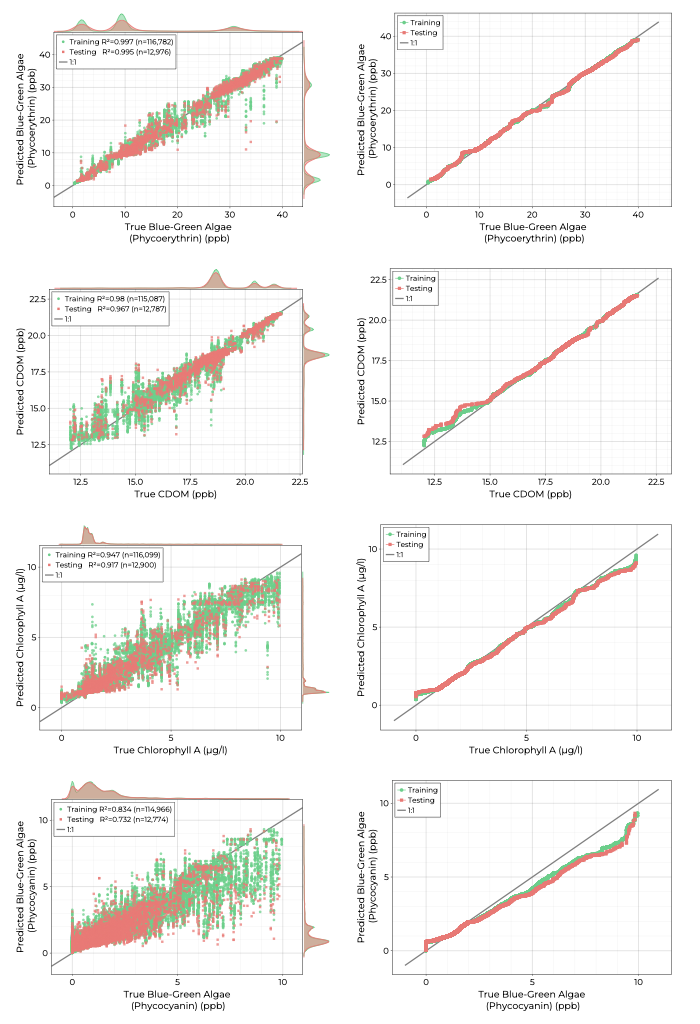
\includegraphics[width=\columnwidth]{robot-team-supervised/results/fits/biochemical-fitres.png}
\vspace{-0.1in}
\caption{Scatter plots (\textbf{left}) and quantile--quantile plots (\textbf{right}) for the final hyperparameter-optimized models for the biochemical targets blue--green algae (phycoerythrin), CDOM, chlorophyll-a, and blue--green algae (phycocyanin). \label{fig:biochem-fit}}
\end{figure}  

\begin{figure}[H]

\vspace{-0.15in}
\hspace{-6pt}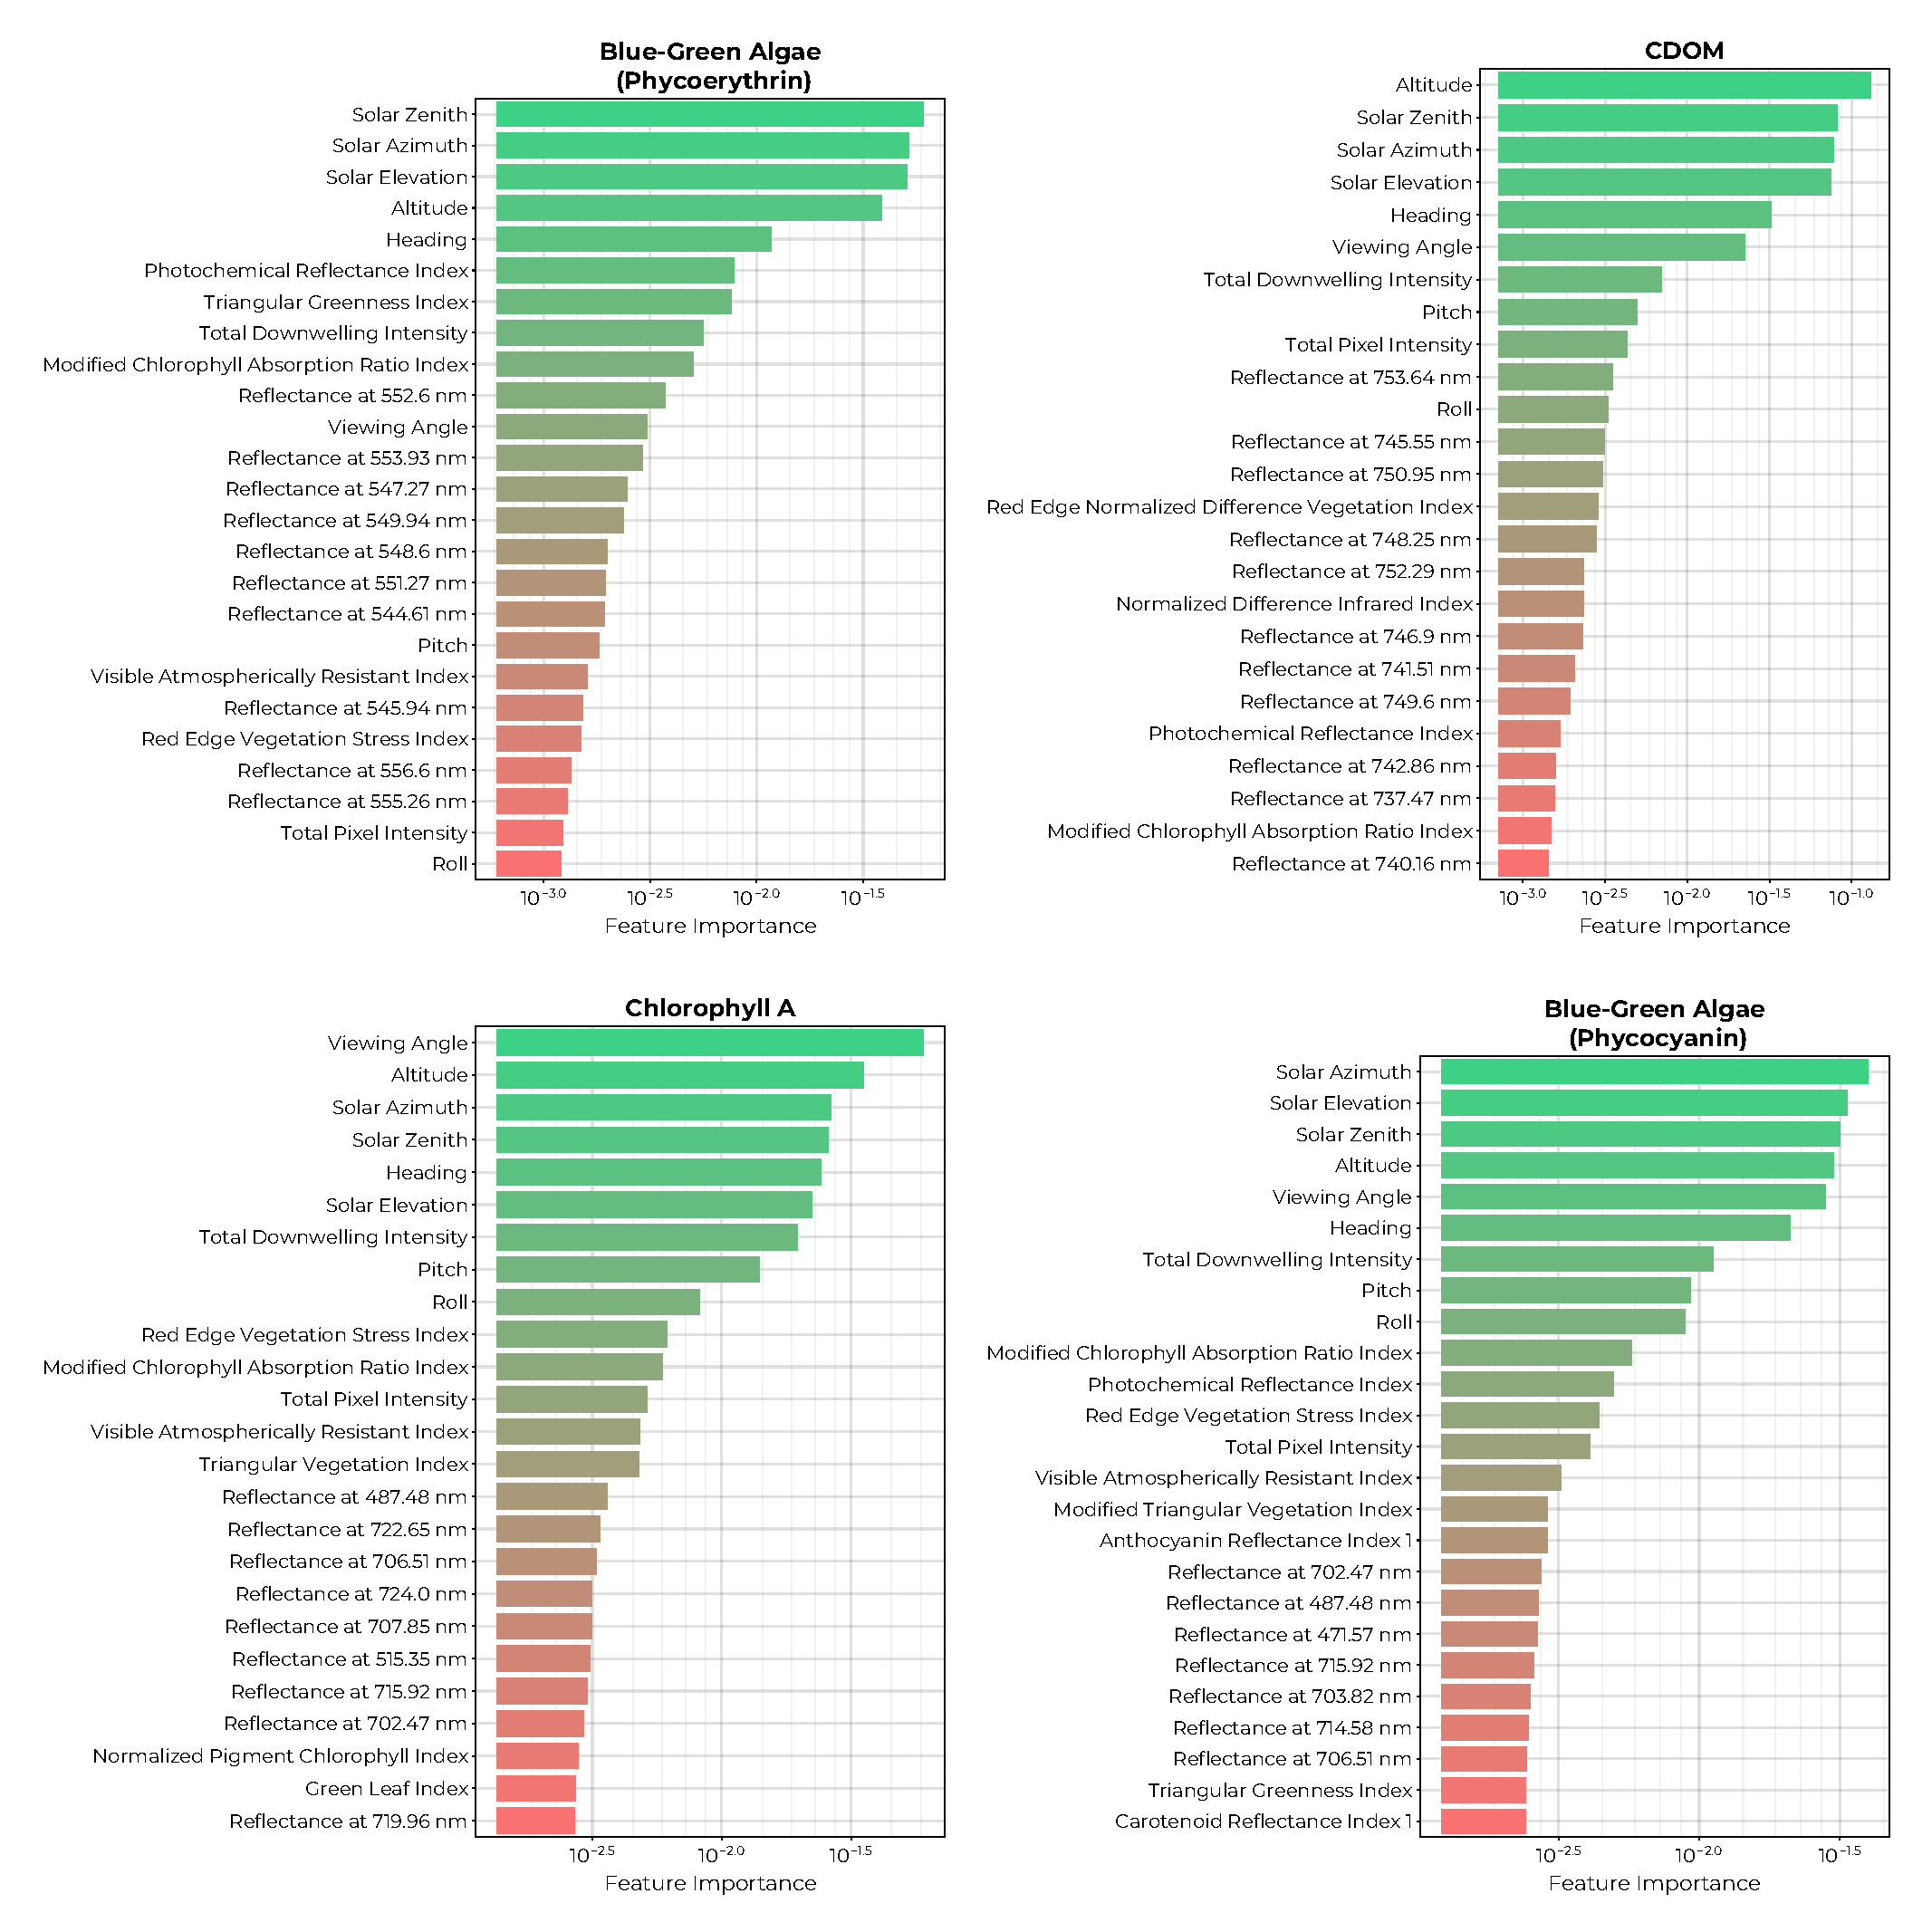
\includegraphics[width=0.9\columnwidth]{robot-team-supervised/results/fits/biochemical-ranking.pdf}
\vspace{-0.1in}
\caption{Ranked permutation importance for each feature in the trained biochemical models. The permutation importance measures the decrease in the model's $R^2$ value after replacing each feature with a random permutation of its values.\label{fig:biochem-fi}}
\end{figure}  


\vspace{-9pt}
\begin{figure}[H]

\vspace{-0.15in}
\hspace{-6pt}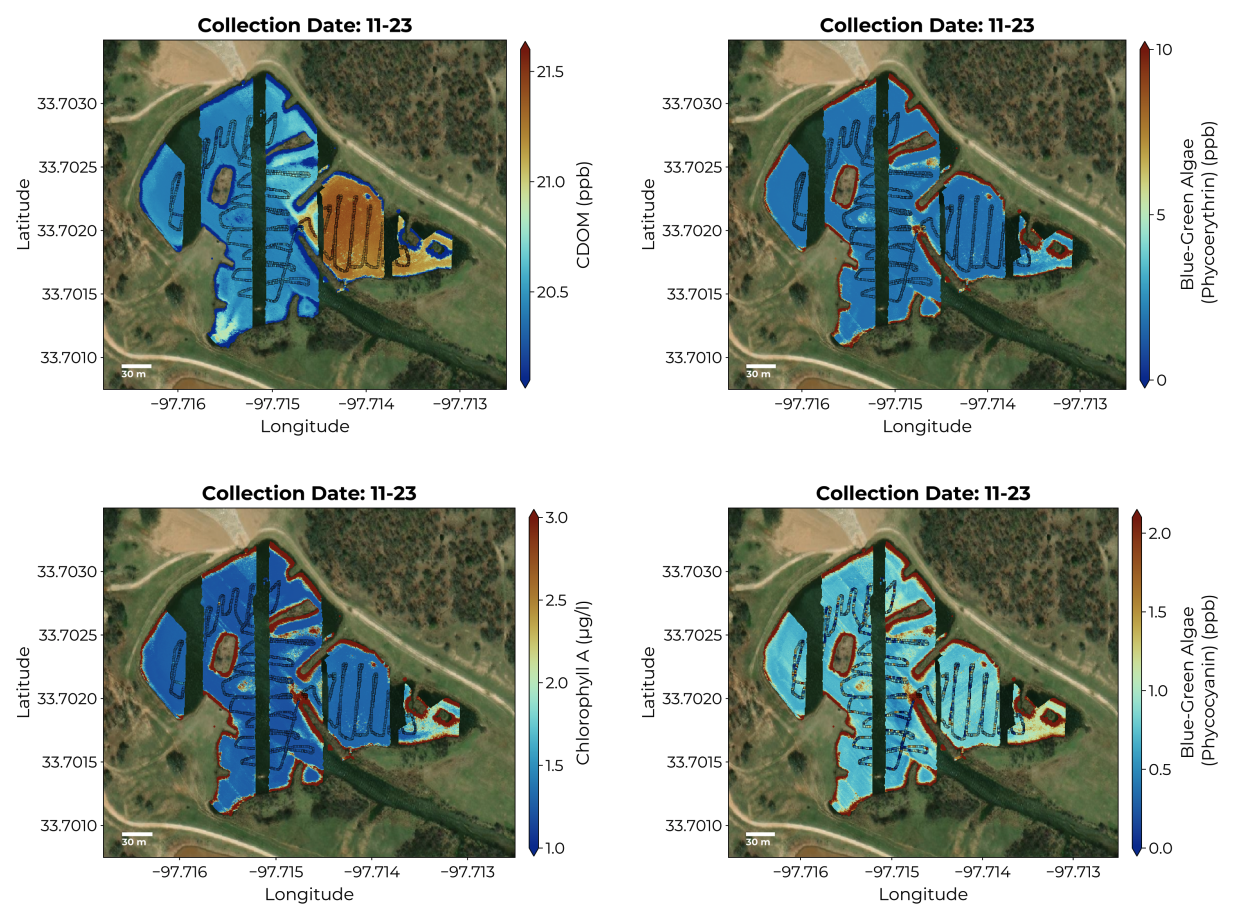
\includegraphics[width=0.92\columnwidth]{robot-team-supervised/results/maps/biochemical.png}
\vspace{-0.1in}
\caption{Maps generated 
 by applying the trained biochemical models to the data cubes collected on 23 November. Overlaid are the in situ reference data for the same collection period. The size of the squares has been exaggerated for the visualization. We note there is good agreement between the predicted map and the reference data. \label{fig:map-biochem}}
\end{figure}  


 

\subsection{Chemical Variables}

The final two models to consider are for the measured chemical concentrations of crude oil (CO) and optical brighteners (OB). The crude oil measurement includes natural unprocessed petroleum, whereas optical brighteners consist of whitening agents that are often added to products such as soaps, detergents, and cleaning agents. Both the crude oil and optical brightener measurements show multi-modal spatial distributions across each collection period. Scatter diagrams and quantile--quantile plots for the fitted models are shown in Figure~\ref{fig:chemicals-fit}. Both models achieve good performance, with $R^2$ values of 0.957 and 0.941 for CO and OB on the holdout test set. The performance of the CO model degrades for concentrations below 24 ppb, for which there are few records. Similarly, the OB model shows worse performance for concentrations below roughly 3.5 ppb.

The ranked permutation importances of the top 25 features for each model are shown in Figure~\ref{fig:chemicals-fi}. Both models rank the solar illumination and viewing geometries together with the total downwelling intensity and total pixel intensities amongst the top features. Both models include a combination of spectral indices using blue, green, yellow, red, and infrared reflectance bins. Additionally, the CO model includes green--yellow reflectances from 539 to 589 nm as well as red reflectances from 749 to 769 nm. The OB model includes yellow reflectance at 584.6 nm and red reflectance bins.

The maps generated by applying the CO and OB models to the 23 November data cubes are shown in Figure~\ref{fig:map-chem}. Both models show a distinct spatial distribution, with elevated values in the eastern alcove of the pond---similar to the CDOM distribution in Figure~\ref{fig:map-biochem}.




% Example of a figure that spans the whole page width. The same concept works for tables, too.
%\begin{figure}[H]
%\centering
%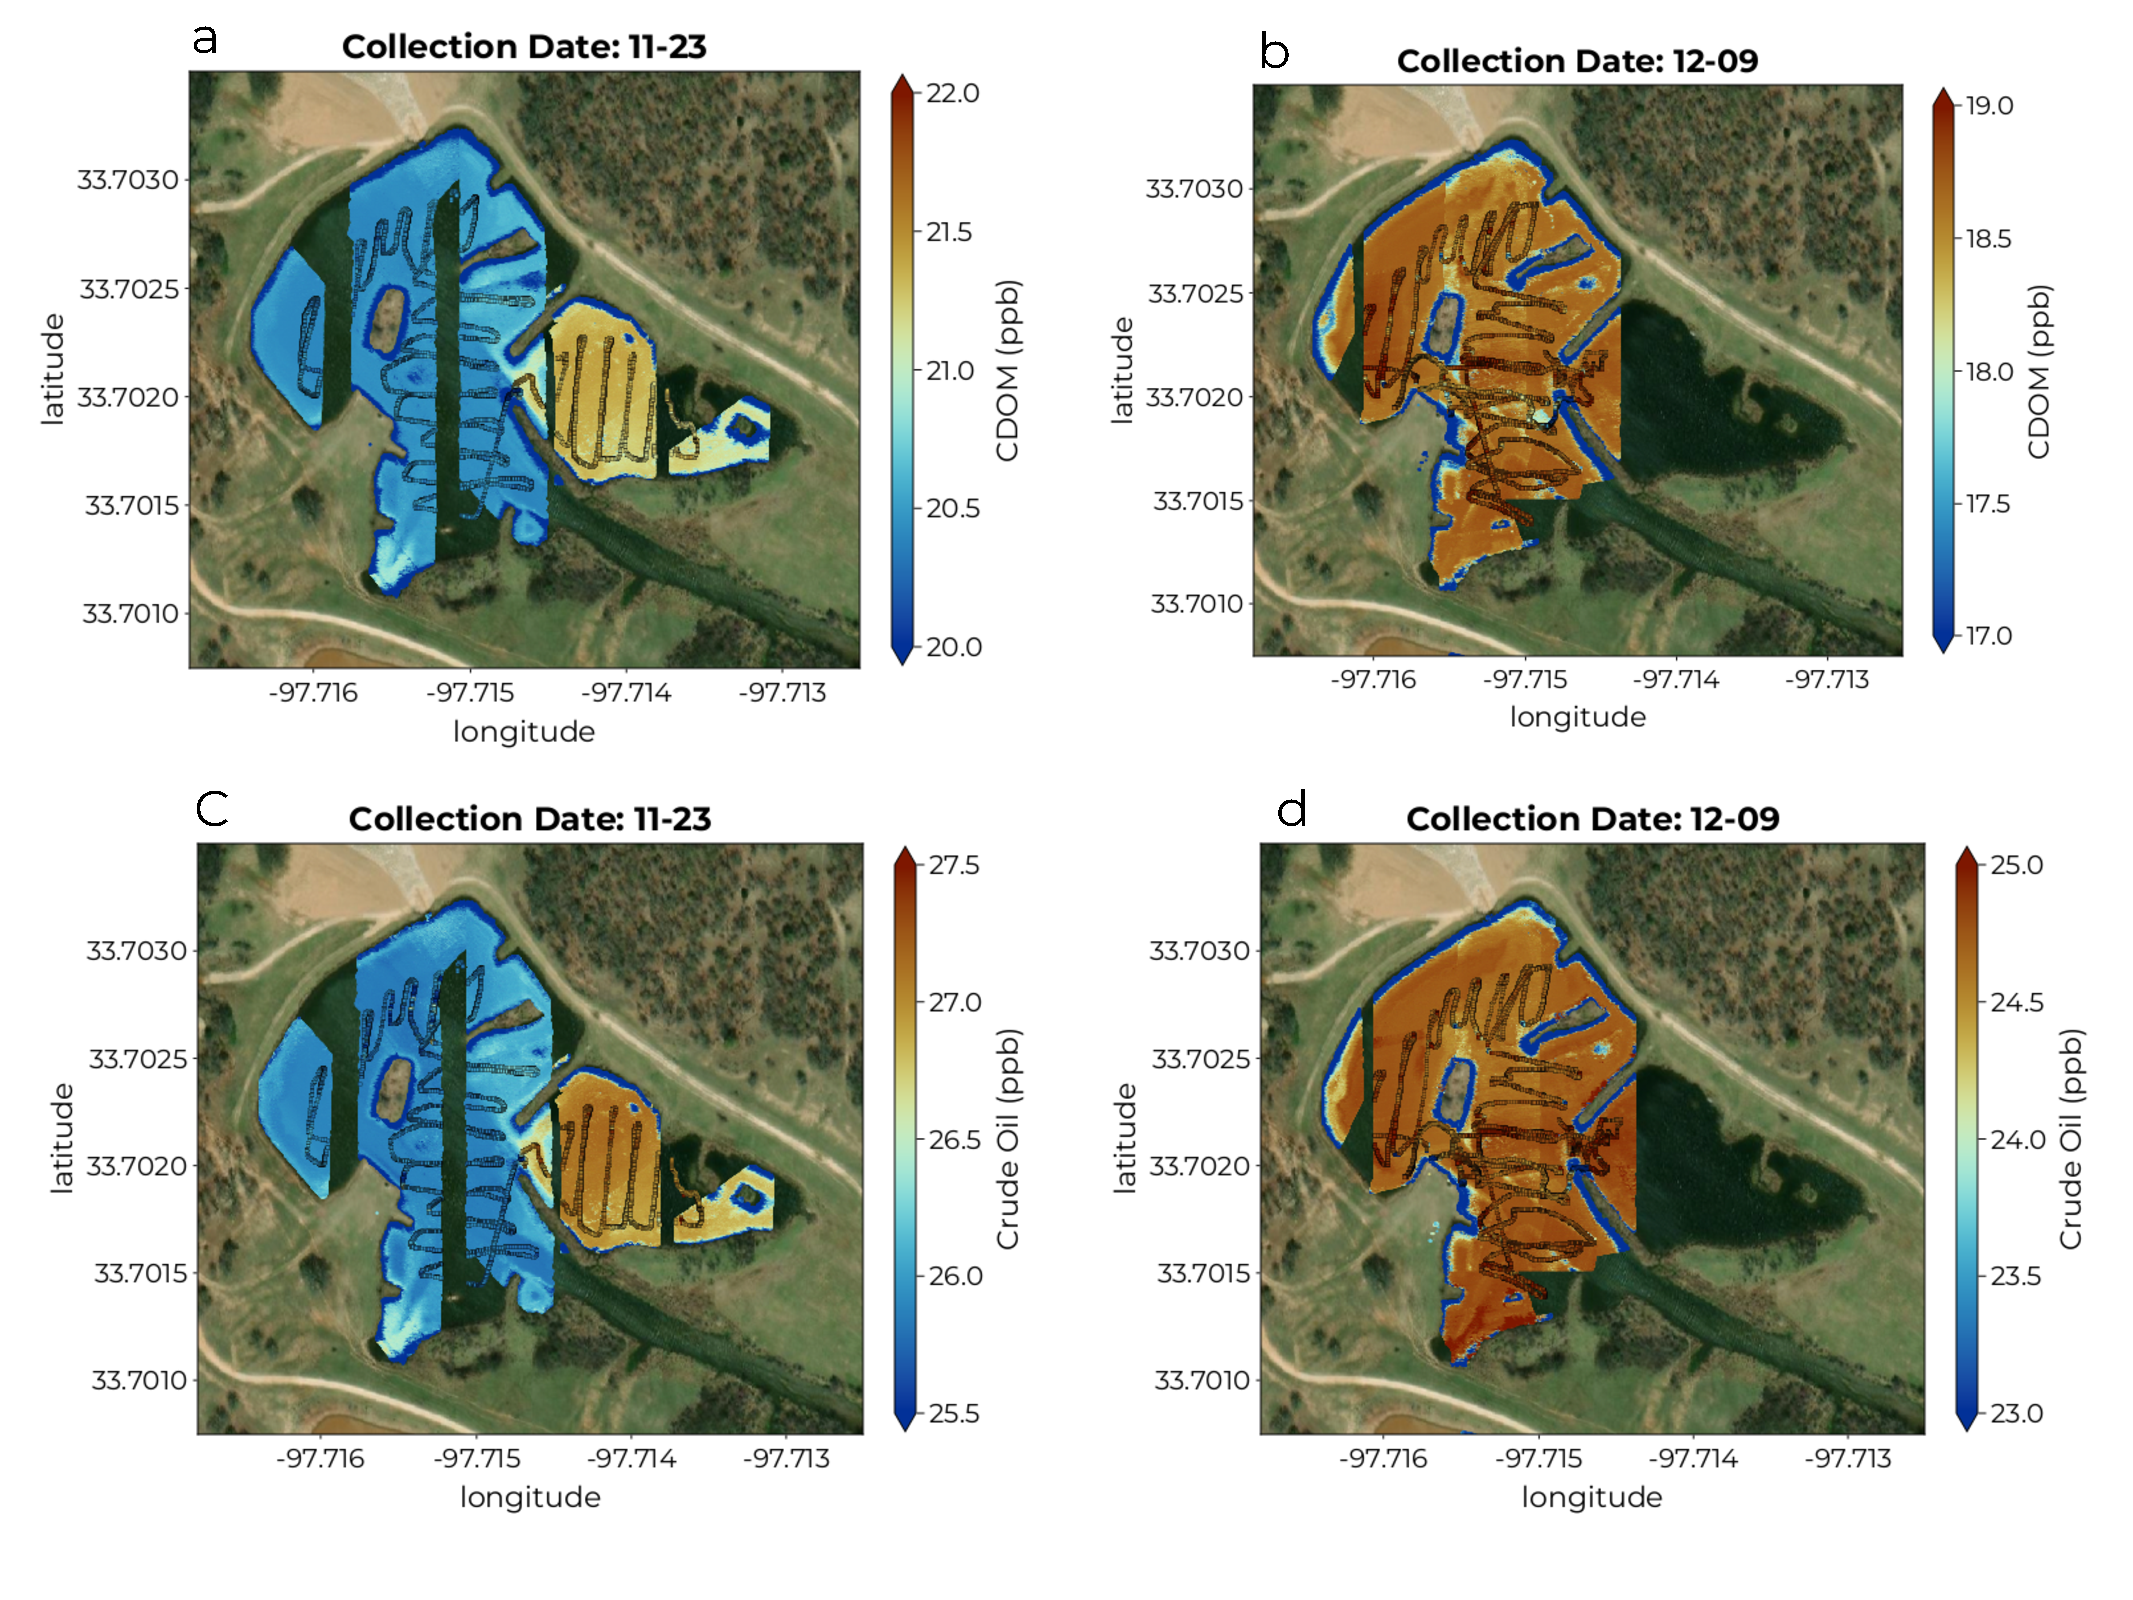
\includegraphics[width=18.0cm]{robot-team-supervised/results/map-combined.pdf}
%\caption{Maps generated by applying the ML model to hyperspectral data cubes. (\textbf{a}) The CDOM model applied to the 11-23 collection. (\textbf{b}) The CDOM model applied the the 12-09 collection. (\textbf{c}) the Crude Oil model applied to the 11-23 collection. (\textbf{d}) The Crude Oil model applied to the 12-09 collection. In each panel, boat data are overlaid as color-filled squares. We note that there is good agreement between estimated values at boat locations and the in situ reference measurements. \label{fig:maps}}
%\end{figure}  
\begin{figure}[H]

\vspace{-0.21in}
\hspace{-6pt}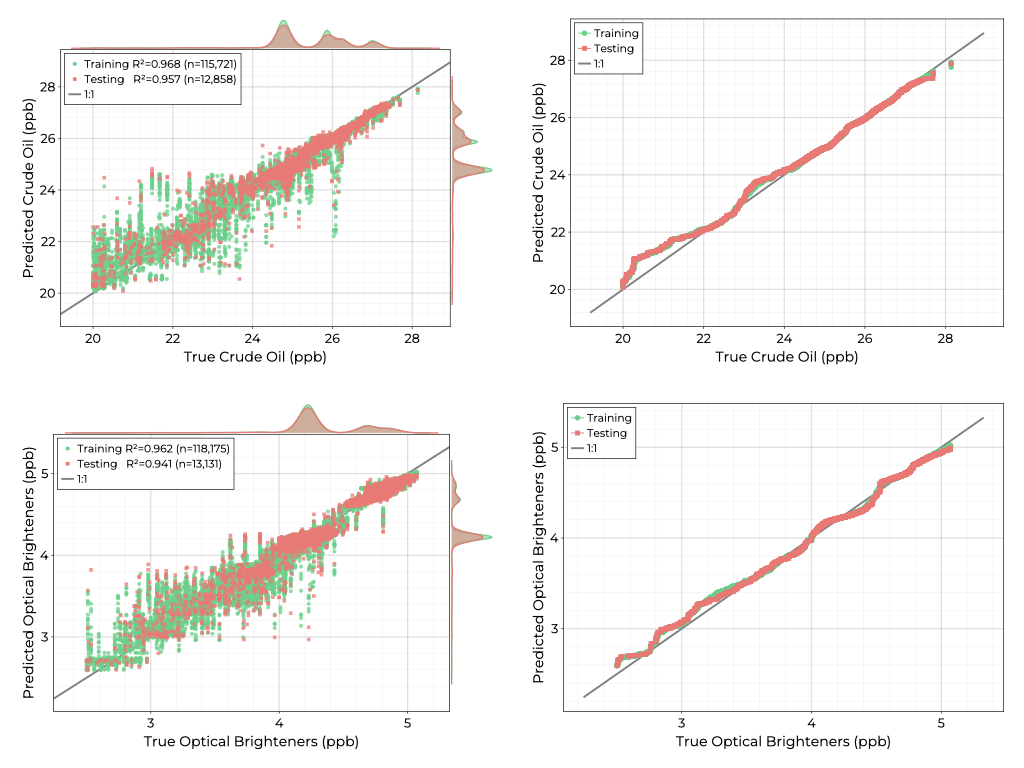
\includegraphics[width=\columnwidth]{robot-team-supervised/results/fits/chemical-fitres.png}
\vspace{-0.11in}
\caption{Scatter diagrams (\textbf{left}) and quantile--quantile plots (\textbf{right}) for the hyperparameter-optimized RFR models for the chemical variables measured by the USV.\label{fig:chemicals-fit}}
\end{figure}  

\vspace{-9pt}
\begin{figure}[H]
\vspace{-0.15in}
\hspace{-6pt}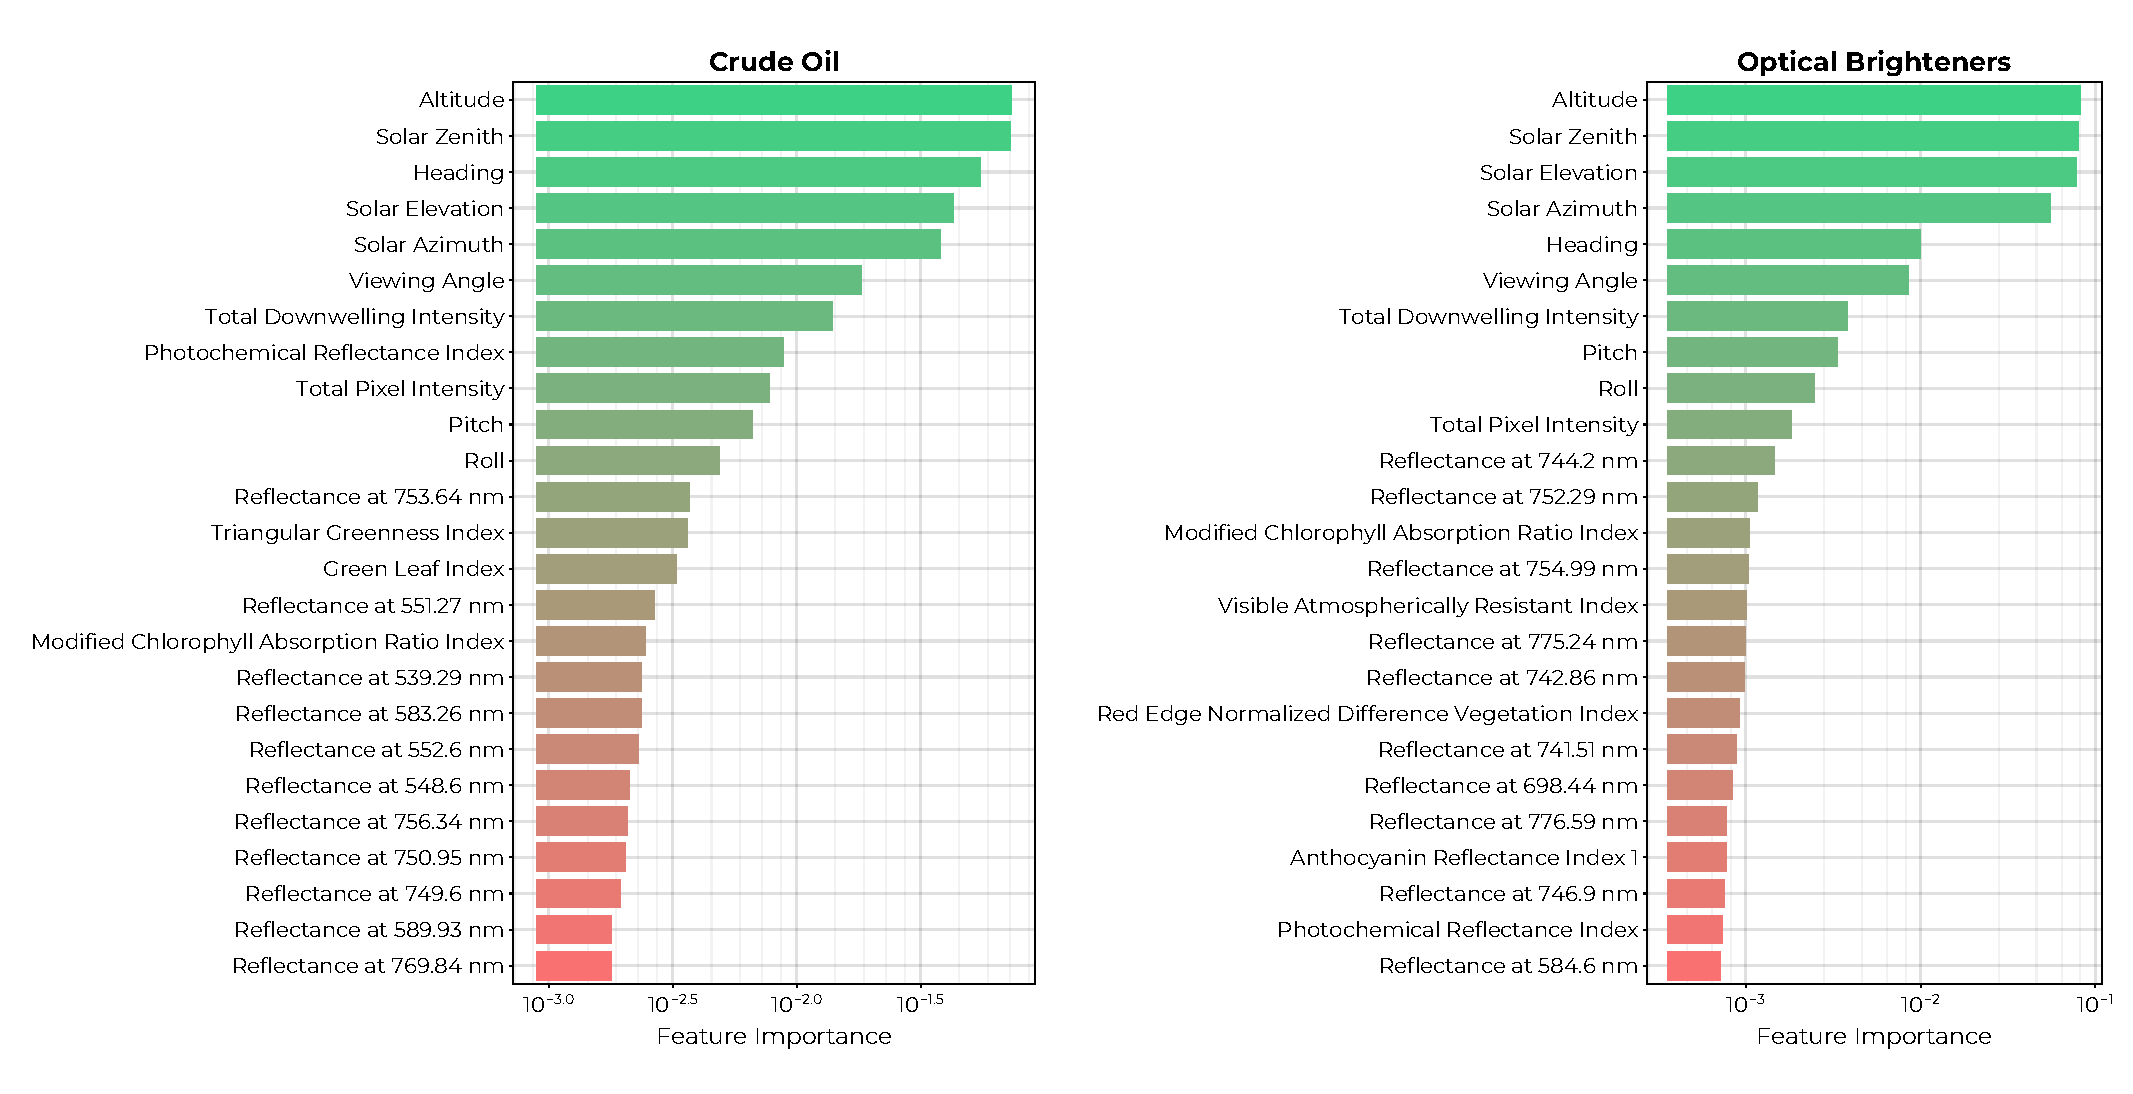
\includegraphics[width=\columnwidth]{robot-team-supervised/results/fits/chemical-ranking.pdf}
\vspace{-0.15in}
\caption{Ranked permutation importance for the top 25 features of the chemical models. The permutation importance measures the decrease in the model's $R^2$ value after replacing each feature in the prediction set with a random permutation of its values.\label{fig:chemicals-fi}}
\end{figure}  

\begin{figure}[H]

\vspace{-0.2in}
\hspace{-6pt}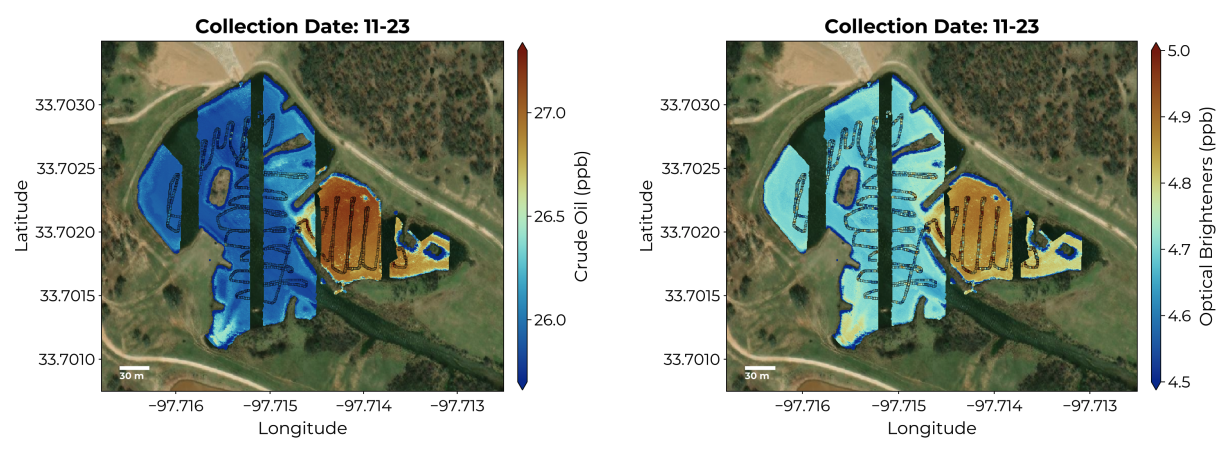
\includegraphics[width=\columnwidth]{robot-team-supervised/results/maps/chemical.png}
\vspace{-0.1in}
\caption{Maps generated by applying the trained chemical variable models to the hyperspectral data cubes collected on 23 November. Overlaid are color-filled squares showing the in situ reference data for the same collection period. The size of the squares is exaggerated for the visualization. We note that there is good agreement between the model predictions and reference data.\label{fig:map-chem}}
\end{figure} 



\section{Discussion}



In recent years, much effort has been spent on the curation of comprehensive datasets combining water quality records with decades of satellite imagery to enable the development of new methods for retrieving water quality parameters. For example, Aurin et al. curated over 30 years of oceanographic field campaign data with associated coincident satellite imagery \cite{aurin2018remote}. Similarly, Ross et al. combined more than 600,000 records of dissolved organic carbon, chlorophyll-a and other water quality variables with historical Landsat reflectance data for the period 1984--2019 \cite{ross2019aquasat}. The sensing paradigm we have demonstrated here was able to rapidly collect comparable volumes of data within the span of just three observation periods. Therefore, despite the fact that individual UAV tracks cover far less spatial extent than remote sensing imagery, the ability to collect coordinated in situ measurements together with detailed hyperspectral images offers a significant improvement over these traditional approaches. With a coordinated robot team, one does not need to rely on infrequent satellite overpasses when planning data collection. Furthermore, the time offset between reference measurements and remote sensing is significantly reduced from days to minutes.

This study is not the first to employ UAVs equipped with multispectral or hyperspectral imagers for the purpose of assessing water composition and quality. Indeed there are many such examples focused on inferring optically active and inactive water quality parameters using band ratios and machine learning methods \cite{vogt2016near,lu2021retrieval, zhang2022selection}. The key advancement demonstrated by our robot team is the ability to combine UAV-borne hyperspectral imagers together with comprehensive, in situ sensing for a significant improvement in data volume. Purposefully coordinating USV sampling with the flight tracks of the UAV greatly accelerates data collection by removing the need to acquire individual samples for the calibration of water quality models. Additionally, the USV facilitates rapid validation of model predictions. When a trained model applied to collected hyperspectral imagery suggests elevated levels of a particular water quality parameter, the USV can quickly be provisioned to confirm these estimates with its reference instruments. 

In \cite{robotTeam1}, we introduced this paradigm. In this study, we have built on this approach in three new ways. First, we have demonstrated the ability to effectively combine observations from disparate collections by augmenting the machine learning models with sufficient features describing the illumination and viewing geometries. As Figure~\ref{fig:downwelling-hist} indicates, we observed variation in the total downwelling intensity between the images collected on the same day and between each separate collection period. These within-collection variations are due to a combination of the stability of the UAV (on which the upward facing downwelling irradiance spectrometer is mounted) together with the occasional interference of clouds. Moreover, the assumption that the water's surface can be treated as Lambertian is clearly violated when the water is not perfectly still. Despite the potential impact of these limitations on the quality of the resulting reflectance data cubes, the smoothness of the maps generated by our models suggests that we have provided sufficient context by including the relevant solar illumination and viewing angles as additional features in the final dataset.  This fact is reinforced by the position of these variables as the most important features for \textit{each} of the estimated water quality variables. As long as we are primarily interested in these values and not the reflectances themselves, we are able to successfully account for these lighting effects when combining data from multiple collections.

The second contribution of this study is to explore the breadth of possible water quality and composition parameters that can be accurately mapped by hyperspectral imagery collected by the UAV. The results presented here confirm the ability of the robot team to predict optically active parameters including blue--green algae, chlorophyll-a, CDOM, crude oil, optical brighteners, turbidity, and temperature. Additionally, we are also able to infer the distributions of optically inactive variables including conductivity, pH, and ion concentrations. Other studies using multispectral and hyperspectral remote sensing imagery have also estimated optically inactive water quality parameters, with the ability to do so stemming from the relationship of these variables to optically active properties of the water \cite{vakili2020determination,guo2021machine,niu2021deep}. We note that in our investigation, the models trained for many of these variables outperformed their optically active counterparts. As the abundance of these variables is likely tied to the specific composition and content of the pond, it is unlikely that models trained for these optically inactive variables will generalize to other bodies of water. 

The third contribution of this work is the extension of our machine learning approach to enable uncertainty quantification through conformal prediction. For water quality risk assessment, the trustworthiness of model predictions is of equal or greater importance to the values themselves. However, robust uncertainty quantification has historically been challenging for many machine learning models, which behave like black boxes.
Conformal prediction is an attractive approach to enable model-agnostic uncertainty estimation and has recently seen adoption to remote sensing classification tasks such as land-type classification and object identification \cite{valle2023quantifying, zhu2024inductive}. In this setting, the goal is to produce predictive sets guaranteed to contain the correct class labels at a predetermined confidence level. Nevertheless, conformal prediction works equally well for regression tasks. By leveraging the large data volume collected by the robot team, we are able to simultaneously train predictive models and evaluate confidence intervals for their predictions. As the final column of Table~\ref{tab:fit-results} confirms, the empirical coverage on the holdout testing set provided by the inferred confidence intervals achieves the desired coverage to within 1\%. We chose to use a 90\% confidence interval for this study, but this can easily be adapted to suite the needs of a specific application if greater confidence is required. 

Despite the wealth of information provided by the increased resolution of hyperspectral images, their considerable size impedes their complete utilization in real-time applications. Often, much of the available spectral information is discarded in favor of indices like the NDVI, which can be quickly computed as images are captured \cite{horstrand2019uav}. Utilizing machine learning allows us to take advantage of the full spectrum captured by each pixel while simultaneously reducing the size of the final data product to single-band ``images'' of selected water quality variables. We note that training a reduced-feature model without further hyperparameter optimization takes roughly one minute per target variable of interest using the processing computer included on the UAV. This means that, in principle, training data can be collected by the USV, imagery can be acquired and processed by the UAV, coincident records can be selected, and the resulting dataset can be used to train machine learning models all while investigators are still in the field. Analyzing the maps produced by applying each trained model enables areas of interest to be readily pinpointed, as demonstrated by the identification of slightly elevated levels of %Please ensure meaning has been retained.
crude oil, optical brighteners, and CDOM in the eastern alcove of the pond on 23 November.

Finally, we note that the high spectral resolution of the UAV imagery together with the ability to collect precisely co-located reference measurements provides fertile ground for the development of new spectral indices targeted towards water quality variables. In this paper, we have shown that permutation importance ranking for trained machine learning models enables a straightforward interpretation of the relative values of each reflectance bin to the final model predictions. In future work, we plan to utilize this information to identify combinations of spectral bands that can be applied to remote sensing imagery captured by satellites equipped with hyperspectral imagers. The recently launched Environmental Mapping and Analysis Program (EnMAP) is one such example and includes over 91 spectral bands in the VNIR that overlap with those of our hyperspectral imager \cite{Storch2023TheEI}. 




\chapter{Unsupervised Characterization of Water Composition with Generative Topographic Mapping}\label{ch:robot-team-gtm}


\section{Motivation}

\section{Unsupervised Learning}

\section{Principal Component Analysis}

\section{Self Organizing Maps}

\section{Generative Topographic Mapping}

\section{Study Overview}

\section{Results}

\section{Discussion}


\chapter{Nonlinear Endmember Extraction and Spectral Unmixing with Generative Simplex Mapping}\label{ch:robot-team-gsm}


\textcolor{red}{In this paper, we introduce a new model for non-linear endmember
  extraction and spectral unmixing of hyperspectral imagery called Generative
  Simplex Mapping (GSM). The model represents endmember mixing using a latent
  space with points sampled within a $(n-1)$-simplex corresponding to the
  abundance of $n$ unique sources. Points in this latent space are non-linearly
  mapped to reflectance spectra via a flexible function combining linear and
  non-linear mixing. Due to the probabilistic formulation of the GSM, spectral
  variability is also estimated by a precision parameter describing the
  distribution of observed spectra. Model parameters are determined using a
  generalized expectation-maximization algorithm. In the event of purely linear
  mixing, non-linear contributions are naturally driven to zero. The GSM
  outperforms three varieties of non-negative matrix factorization for both
  endmember extraction accuracy and abundance estimation on a synthetic data set
  of linearly mixed spectra from the USGS spectral library. In a second
  experiment, the GSM is applied to real hyperspectral imagery captured over a
  pond in North Texas. The model is able to accurately identify spectral
  signatures corresponding to near-shore algae, water, and rhodmaine tracer dye
  introduced into the pond to simulate water contamination by a localized
  source. Abundance maps generated using the GSM accurately track evolution of
  the dye plume as it mixes into the surrounding water.}



\section{Motivation}


Hyperspectral imaging has emerged as a keystone technology in remote sensing, where the ability to discern variations between high-resolution spectra supports a plethora of critical applications such as environmental monitoring, biodiversity conservation, sustainable agriculture, and more. In recent years, many remote sensing platforms have been deployed with hyperspectral imaging payloads such as the Italian PRISMA mission launched in 2019, the German EnMAP launched in 2022, and recently NASA's PACE satellite launched in 2024 \cite{PRISMA-orig, EnMAP-orig, PACE-orig}. Many future missions also plan to incorporate hyperspectral imaging capabilities such as the European Space Agency's CHIME which will include over $200$ bands spanning visible, near-infrared (NIR), and short-wave infrared (SWIR) wavelengths \cite{CHIME-orig}. The continued development of hyperspectral imaging technology has also led to a considerable reduction in size that enables its inclusion in the payloads of small unmanned aerial vehicles (UAVs) \cite{adao2017hyperspectral, arroyo2019implementation}. Despite the proliferation of hyperspectral imaging data sources, the considerable increase in data volume associated with hyperspectral images (HSI) poses significant challenges to real-time analysis at scale.

Many approaches have been developed to make sense of the HSI data. For example, spectral indices such as the popular normalized difference vegetation index (NDVI) can be computed by taking ratios of spectral bands tailored to track specific reflectance characteristics \cite{thenkabail-indices,thenkabail2018hyperspectral}. These indices have the advantage of being easy to compute, but suffer from significant variability between instruments while ignoring most of the information captured in HSI spectra \cite{ndvi-variability}. An alternative approach is to pair HSI data with in situ measurements to enable supervised models that map spectra directly to parameters of interest. However, this approach relies on serendipitous satellite overpasses above sensing sites to generate sufficient quantities of aligned data for model training and evaluation. For example, Aurin et al. combined data from over 30 years of oceanographic field campaigns with paired satellite imagery to develop robust models for the inversion of key water quality indicators such as colored dissolved organic matter \cite{aurin2018remote}. This approach can be accelerated by combining UAV-based hyperspectral imaging with rapid in situ data collection using autonomous boats \cite{robot-team-1, robot-team-2}. However, these supervised methods rely on \textit{a priori} knowledge of expected sources to identify appropriate reference sensors for data collection. In light of these limitations, unsupervised methods are needed that can expediently extract source signatures from high-dimensional HSI.

The spatial resolution of hyperspectral imagers generally results in pixels with mixed signals from multiple sources called endmembers. The task of unsupervised source identification using HSI data therefore involves two steps: endmember extraction and abundance estimation. Techniques such as vertex component analysis (VCA), the pixel purity index (PPI), and N-FINDR solve this first task by identifying HSI endmember spectra assuming the presence of some pure (unmixed) pixels \cite{vca-orig, ppi-orig, N-FINDR-orig}. By further assuming a linear mixing model (LMM) in which observed spectra are described by a linear combination of endmembers with non-negative abundances, HSI can be unmixed using a variety of techniques such as constrained least squares \cite{spectral-unmixing-orig, fcls-unmixing}. Among these methods, Nonnegative Matrix Factorization (NMF) is a widely used approach which extracts endmember spectra and unmixes abundances simultaneously via matrix factorization \cite{nmf-orig, unmixing-nmf-review, unmixing-nmf-review-2}. The update equations for NMF can be formulated as multiplicative updates which guarantee the non-negativity of endmember spectra and their associated abundances \cite{nmf-algorithms}.  For this reason, the continued development of new NMF varieties remains an active area of research.

In realistic scenes, multiple scattering and surface variability can easily challenge the assumption of linear mixing \cite{heylen2014review}. Water-based HSI specifically are prone to non-linear mixing effects due to absorption features of dissolved and suspended substances, fluorescence of organic matter, and particulate scattering in turbid waters \cite{hsi-absorption, hsi-fluorescence, hsi-turibidity}. With the growing popularity of deep learning approaches in remote sensing, a variety of models based on autoencoder architectures have been introduced for unmixing HSI data \cite{non-negative-autoencoders,su2019daen,borsoi2019deep,palsson2020convolutional}. However, the complexity introduced by these models significantly impacts training time and decreases the interpretability of the model. An ideal approach should enable both endmember extraction and non-linear unmixing while accounting for spectral variability. 

The self-organizing map (SOM) is an unsupervised machine learning method that maps high-dimensional data to a low-dimensional grid while preserving the topological relationships between data points \cite{kohonen-som-1}. This low-dimensional representation provides a convenient way to visualize HSI data while the weight vectors for each SOM node can be interpreted as representative spectra \cite{cantero2004analysis, duran2007time,som-hsi}. If labelled reference spectra are available, the SOM can be used to enable semi-supervised labeling of HSI pixels \cite{riese2019supervised}. The SOM has also been shown to be effective for the compression of HSIs acquired by a CubeSat \cite{som-satellite}. Despite these capabilities, the SOM does not offer a probabilistic interpretation and relies on a heuristic training procedure with hyperparameters that can be challenging to tune. To address these shortcomings, Bishop et al. introduced the Generative Topographic Mapping (GTM), a probabilistic latent-variable model inspired by the SOM \cite{gtm-orig}. When choosing a two-dimensional latent space, the GTM can be used to visualize the distribution of HSI spectra while mapping the latent space nodes to the HSI data space provides endmembers \cite{robot-team-gtm}. Unfortunately, the rectangular latent space grid employed by the GTM does not directly translate into endmember abundances. Additionally, the expectation-maximization (EM) algorithm used to train the GTM does not guarantee non-negativity of GTM node spectra. 

In this paper, we introduce a new variant of the GTM dubbed Generative Simplex Mapping (GSM), which can extract endmember spectra and unmix non-linear mixtures. By replacing the rectangular latent space of the GTM with a gridded $n$-simplex, the vertices of the GSM can be immediately interpreted as endmembers corresponding to $n+1$ unique spectral signatures. The mapping from the latent space to the HSI data space models signal mixing while barycentric coordinates for the latent space simplex estimate relative endmember abundances. Furthermore, by taking inspiration from the multiplicative updates of NMF, the GSM algorithm maintains the non-negativity of resulting endmember spectra. If only linear mixing is present, the GSM algorithm drives non-linear contributions to $0$. Prior distributions included for GSM model weights yield hyperparameters which can be tuned to control the smoothness of the resulting spectra and the degree of non-linear mixing applied.

% The remainder of the paper is structured as follows. Section~\ref{sec:gsm} describes the proposed method. Section~\ref{sec:experiments} and Section~\ref{sec:results} describe experiments using real and simulated HSI data to evaluate the GSM model. Section~\ref{sec:disucssion} discusses additional applications and extensions of the GSM to be explored in future work. Finally, Section~\ref{sec:conclusions} finishes the paper with some closing remarks.



\section{Spectral Mixing}

Linear Mixing
Bilinear Mixing
Postlinear Polynomial Mixing

\subsection{Popular Models}
NCA, PPI, MVF, Autoencoders, etc...

\section{Nonnegative Matrix Factorization}

\section{GSM}

In the original GTM formulation, the data vectors $x$ (reflectance spectra) are described by latent variables $z$ mapped into the data space by a non-linear function $\psi$. The data space distribution is taken to be normal with the precision parameter $\beta$ to account for measurement noise and spectral variability. The GSM uses same structure, that is
\begin{equation}\label{eqn:data-space-distribution}
    p(x \mid z, \mathbf{W}, \beta) = \left(\frac{\beta}{2\pi} \right)^{D/2}\exp\left( -\frac{\beta}{2}\lVert \psi(z; \mathbf{W}) - x \rVert^2 \right)
\end{equation}
where $\mathbf{W}$ are model weights which parameterize the mapping $\psi$.

Assuming data are uniformly sampled from an embedded manifold in the data space, the GTM models the latent space using a rectangular grid with $K$-many nodes of equal prior probability. To adapt the GTM to describe endmember mixing, the GSM makes two key changes. The first is to replace the rectangular GTM grid with a gridded simplex with $N_v$ vertices. The barycentric coordinates for each node then describe the relative abundance of each endmember with each vertex corresponding to a pure endmember. The second change is to replace equal prior probabilities with adaptive mixing coefficients $\pi_k$ to allow the GSM to model HSI with nonuniform mixing distributions. Together, this leads to a latent space prior distribution given by
\begin{equation}\label{eqn:latent-distribution}
    p(z) = \sum\limits_k^K \pi_k \, \delta(z - z_k) \quad\text{where}\quad  \sum_k^K\pi_k = 1.
\end{equation}

For a data set containing $N$-many records, these definitions yield a log likelihood function given by
\begin{equation}\label{eqn:llh}
    \mathcal{L} = \sum\limits_n^N \ln \left( \sum\limits_k^K \pi_k \, p(x_n \mid z_k, \mathbf{W}, \beta) \right)
\end{equation}
which can be maximized to obtain optimal values for model weights $\mathbf{W}$, mixing coefficients $\pi_k$, and precision $\beta$. Rather than optimizing Eq~\ref{eqn:llh} directly, we instead choose a particular form for $\psi$ to allow fitting the GSM via an EM algorithm.

In the standard LMM model, the mapping $\psi$ is given by $\psi(z;W) = \mathbf{W}z$ where the columns of $\mathbf{W}$ correspond to endmember spectra. To model non-linear mixing, $z$ is replaced by the output of $M$-many activation functions such that $\psi(z;W) = \mathbf{W}\phi(z)$. The activations applied to each GSM node can then be collected to form a matrix with elements $\Phi_{km} = \phi_m(z_k)$. For $m \leq N_v$, we take $\Phi_{km} = z_k$ to model linear mixing. The remaining  $M-N_v$ activations are computed using radial basis functions (RBF) with centers $\mu_m$ distributed throughout the simplex (but not at the vertices) with 
\begin{equation}\label{eq:act-function}
    \Phi_{km} = \begin{cases}
        \dfrac{s - \lVert z_k - \mu_m \rVert}{s}; & \lVert z_k - \mu_m \rVert \leq s \\
        0; & \lVert z_k - \mu_m \rVert > s
    \end{cases}
\end{equation}
where $s$ is the spacing between RBF centers. In this form, the first $N_v$ columns of $\mathbf{W}$ correspond to endmember spectra, while the remaining columns account for additional non-linear effects. For linear mixing, the GSM training algorithm should therefore drive $W_{dm}$ to $0$ for $m\geq N_v$. A visualization of the GSM model is shown in Figure~\ref{fig:gsm-diagram}.


\begin{figure}[H]
  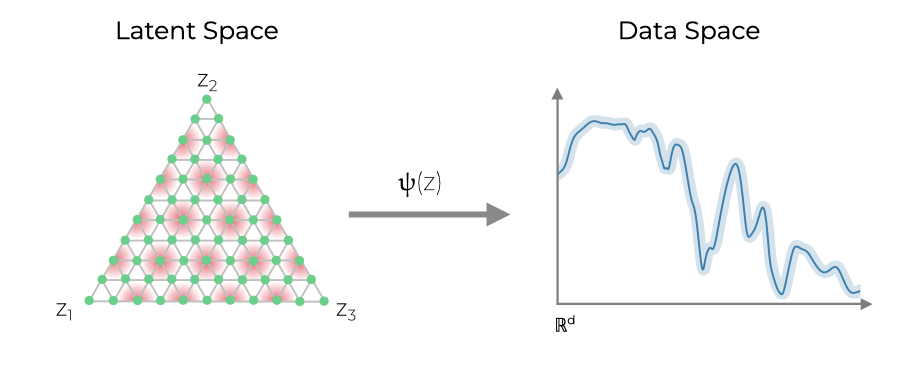
\includegraphics[width=\columnwidth]{robot-team-gsm/methods/gsm/gsm-diagram.png}
  \caption{Illustration of the GSM. The latent space consists of a grid of
    $K$-many points (green dots) distributed throughout a simplex with $N_v$
    vertices. Barycentric coordinates of each node in the simplex correspond to
    the relative abundance of $N_v$-many unique sources. Here, $N_v=3$ has been
    chosen for illustrative purposes. Nodes are mapped into the data space via
    the map $\psi(z)$ utilizing $M$-many radially symmetric basis functions
    (red). Spectral variability is estimated via the precision parameter $\beta$
    shown here in the data space as a light blue band around the spectrum given
    by $\psi(z)$.}
  \label{fig:gsm-diagram}
\end{figure}  

To further constrain the model, we introduce prior distributions on the weights $\mathbf{W}$. For $m\leq N_v$ we take $W_{dm}\sim\mathcal{N}(0, \lambda_e^{-1})$ corresponding to a zero-mean Gaussian with variance $\lambda_e^{-1}$. For $m>N_v$ we use a zero-mean Laplace distribution, $W_{dm}\sim\dfrac{\lambda_w}{2}\exp(-\lambda_w\lvert W_{dm}\rvert)$, with scale parameter $\lambda_w^{-1}$. Under these choices $\lambda_e$ corresponds to $L_2$ regularization on endmember spectra while $\lambda_w$ corresponds to $L_1$ regularization on the non-linear activations. In other words, $\lambda_e$ governs the smoothness of the resulting endmembers while $\lambda_w$ encourages sparsity for the non-linear contributions.

An EM algorithm for the GSM model can now be formulated as follows. Suppose that we have current estimates for the model weights $\mathbf{W}$, mixing coefficients $\pi_k$, and precision parameter $\beta$. During the expectation step we compute the posterior probabilities, that is, the responsibility of each GSM node for each spectrum in the data set:
\begin{equation}\label{eq:responsibility}
    R_{kn}  = p(z_k \mid x_n, \mathbf{W}, \beta) = \dfrac{\pi_k \, p(x_n \mid z_k, \mathbf{W}, \beta)}{\sum\limits_{k'}^K \pi_{k'} \, p(x_n \mid z_{k'}, \mathbf{W}, \beta)}.
\end{equation}
For the maximization step, we consider the expectation of the penalized complete-data log likelihood given by
\begin{equation}\label{eq:complete-data-llh}
\begin{aligned}
    Q &= \sum_n^N\sum_k^K R_{kn} \left(\ln\pi_k + \frac{D}{2}\ln\left(\frac{\beta}{2\pi}\right) - \frac{\beta}{2}\sum_d^D\left(\sum_m^M W_{dm}\Phi_{km} - X_{nd}\right)^2\right) \\ 
    &\qquad + \frac{N_vD}{2}\ln\left(\frac{\lambda_e}{2\pi}\right) - \frac{\lambda}{2}\sum_d^D \sum_{m=1}^{N_v} W_{dm}^2  \\ 
    &\qquad + (M-N_v)D\ln\left(\dfrac{\lambda_w}{2}\right) - \lambda_w\sum_d^D\sum_{m=N_v+1}^{M} W_{dm}
\end{aligned}
\end{equation}
where $X_{nd}$ is the $d$-th component of the $n$-th spectrum in the data set. Eq~\ref{eq:complete-data-llh} is then maximized with respect to $\pi_k$, $\beta$, and $\mathbf{W}$ to obtain new parameter values. For a detailed overview of the EM procedure, the reader is directed to ref. \cite{bishop-prml}.

For $\pi_k$, optimization can be performed using Lagrange multipliers to maintain the condition that $\sum_k\pi_k=1$. Doing so yields
\begin{equation}\label{eq:pi-update}
    \pi_k^{\text{new}}  = \frac{1}{N}\sum_n R_{kn}
\end{equation}

Optimization of Eq~\ref{eq:complete-data-llh} with respect to $\mathbf{W}$ leads to a linear system which can be solved using standard numerical methods. However, in this form, we cannot guarantee the non-negativity of $\mathbf{W}$ required to describe reflectance spectra. Therefore, we take inspiration from the multiplicative updates for NMF introduced by Lee and Seung \cite{nmf-orig}. A standard gradient-based update for $\mathbf{W}$ would normally take the form
\begin{equation}
    \mathbf{W}_{\text{new}} = \mathbf{W} + \eta\frac{\partial Q}{\partial \mathbf{W}}
\end{equation}
for some learning rate $\eta$. Therefore, we differentiate to obtain
\begin{equation}
    \frac{\partial Q}{\partial \mathbf{W}} = -\beta \mathbf{W}\mathbf{\Phi}^T\mathbf{G}\mathbf{\Phi} - \mathbf{\Lambda} + \beta \mathbf{X}^T\mathbf{R}^T\mathbf{\Phi}
\end{equation}
where $\mathbf{G}$ is a diagonal matrix with $G_{kk} = \sum_n R_{kn}$ and $\mathbf{\Lambda}$ is given by 
\begin{equation}
    \Lambda_{dm} = \begin{cases}
        \lambda_e W_{dm}; & m \leq N_v \\ 
        \lambda_w; & m > N_v
    \end{cases}
\end{equation}
If we allow individual learning rates $\eta_{dm}$ for each element of $\mathbf{W}$, then choosing 
\begin{equation}
    \eta_{dm} = \frac{W_{dm}}{\left(\beta \mathbf{W}\mathbf{\Phi}^T\mathbf{G}\mathbf{\Phi}\right)_{dm} + \Lambda_{dm}}
\end{equation}
results in a multiplicative update rule given by
\begin{equation}\label{eq:W-update}
    W_{dm}^{new}  = W_{dm} \cdot \dfrac{\left(\beta \mathbf{X}^T\mathbf{R}^T\mathbf{\Phi}\right)_{dm}}{\left(\beta \mathbf{W}\mathbf{\Phi}^T\mathbf{G}\mathbf{\Phi}\right)_{dm} + \Lambda_{dm}}
\end{equation}
From Eq~\ref{eq:W-update}, it is clear that we are multiplying $W_{dm}$ by strictly non-negative values, and therefore, non-negative $W_{dm}$ will remain so during each update. This update can also be repeated multiple times during each M-step to accelerate convergence.

Optimizing Eq~\ref{eq:complete-data-llh} with respect to $\beta$ yields the final update equation:
\begin{equation}\label{eq:beta-update}
    \frac{1}{\beta^{\text{new}}}  = \frac{1}{ND}\sum\limits_n^N\sum\limits_k^K R_{kn}\lVert \psi(z_k; \mathbf{W}) - x_n \rVert^2.
\end{equation}

To train a GSM model, weights $\mathbf{W}$ are randomly initialized to positive values. The mixing coefficients are initially set to $\pi_k = 1/K$. Finally, the precision parameter $\beta$ is initialized to the variance of the $(N_v+1)$-th principal component. After initialization, the expectation and maximization steps are repeated in turn until $Q$ converges to a predetermined tolerance level. For large $N_v$ we note that generating a regular grid within the simplex becomes cumbersome as the number grid nodes scales as ${k + N_v - 2 \choose N_v - 1}$ for $k$ nodes per edge. An alternative approach is to randomly sample points within the simplex to obtain a total of $K$ nodes. A Dirichlet distribution 
\begin{equation}
    p(z_1,...z_{N_v}) = \frac{\Gamma(\sum_i^{N_v}\alpha_i)}{\prod_{i}^{N_v}\Gamma(\alpha_i)} \prod_{i}^{N_v} z_i^{\alpha_i-1}
\end{equation}
with all $\alpha_i=1$ can be used to uniformly sample within the simplex. Since the mixing coefficients $\pi_k$ are adaptive, variability in node separation should not significantly impact the resulting GSM.

The probabilistic form of the GSM means that a variety of information criteria can be used to evaluate the model fits. In this paper we consider two metrics, the Bayesian Information Criterion (BIC),
\begin{equation}
   \text{BIC} = P\ln(N) - 2\mathcal{L},
\end{equation}
and the Akaike Information Criterion (AIC),
\begin{equation}
    \text{AIC} = 2P - 2\mathcal{L}
\end{equation}
where $P$ is the total number of model parameters and $\mathcal{L}$ is the log likelihood from Eq~\ref{eqn:llh}.

The map $\psi$ provides the representation of each node $z_k$ in the data space. Importantly, applying $\psi$ to each vertex extracts endmember spectra from the GSM. Slices $R_{\left[:,n\right]}$ of the matrix $\mathbf{R}$ define the responsibility of each latent node $z_k$ for the $n$-th spectrum $x_n$ in the data set. Therefore once the GSM has been trained, $\mathbf{R}$ can be used to unmix endmember abundances by representing each record in the latent space via the mean: 
\begin{equation}
    \hat{z}_n = \sum_k^K R_{kn}z_k.
\end{equation}

A freely available implementation of the GSM is provided at \cite{gtm-code}. The code is written in the Julia programming language and follows the Machine Learning in Julia (MLJ) common interface \cite{bezanson2012julia, blaom2020mlj}.





\section{Study Overview}


To illustrate the effectiveness of the GSM, we first demonstrate its ability to model simple linear mixing by driving non-linear weights to zero during the fitting process. To this end, a synthetic data set comprising linear mixtures of three sample spectra from the U.S. Geological Survey digital spectral library was generated by sampling $1000$ abundance vectors from a Dirichlet distribution with $\alpha_1=\alpha_2=\alpha_3=1/3$ \cite{usgs-spectra}. These source spectra and abundances are visualized in Figure~\ref{fig:usgs-data}.

\begin{figure}[H]
  \centering
  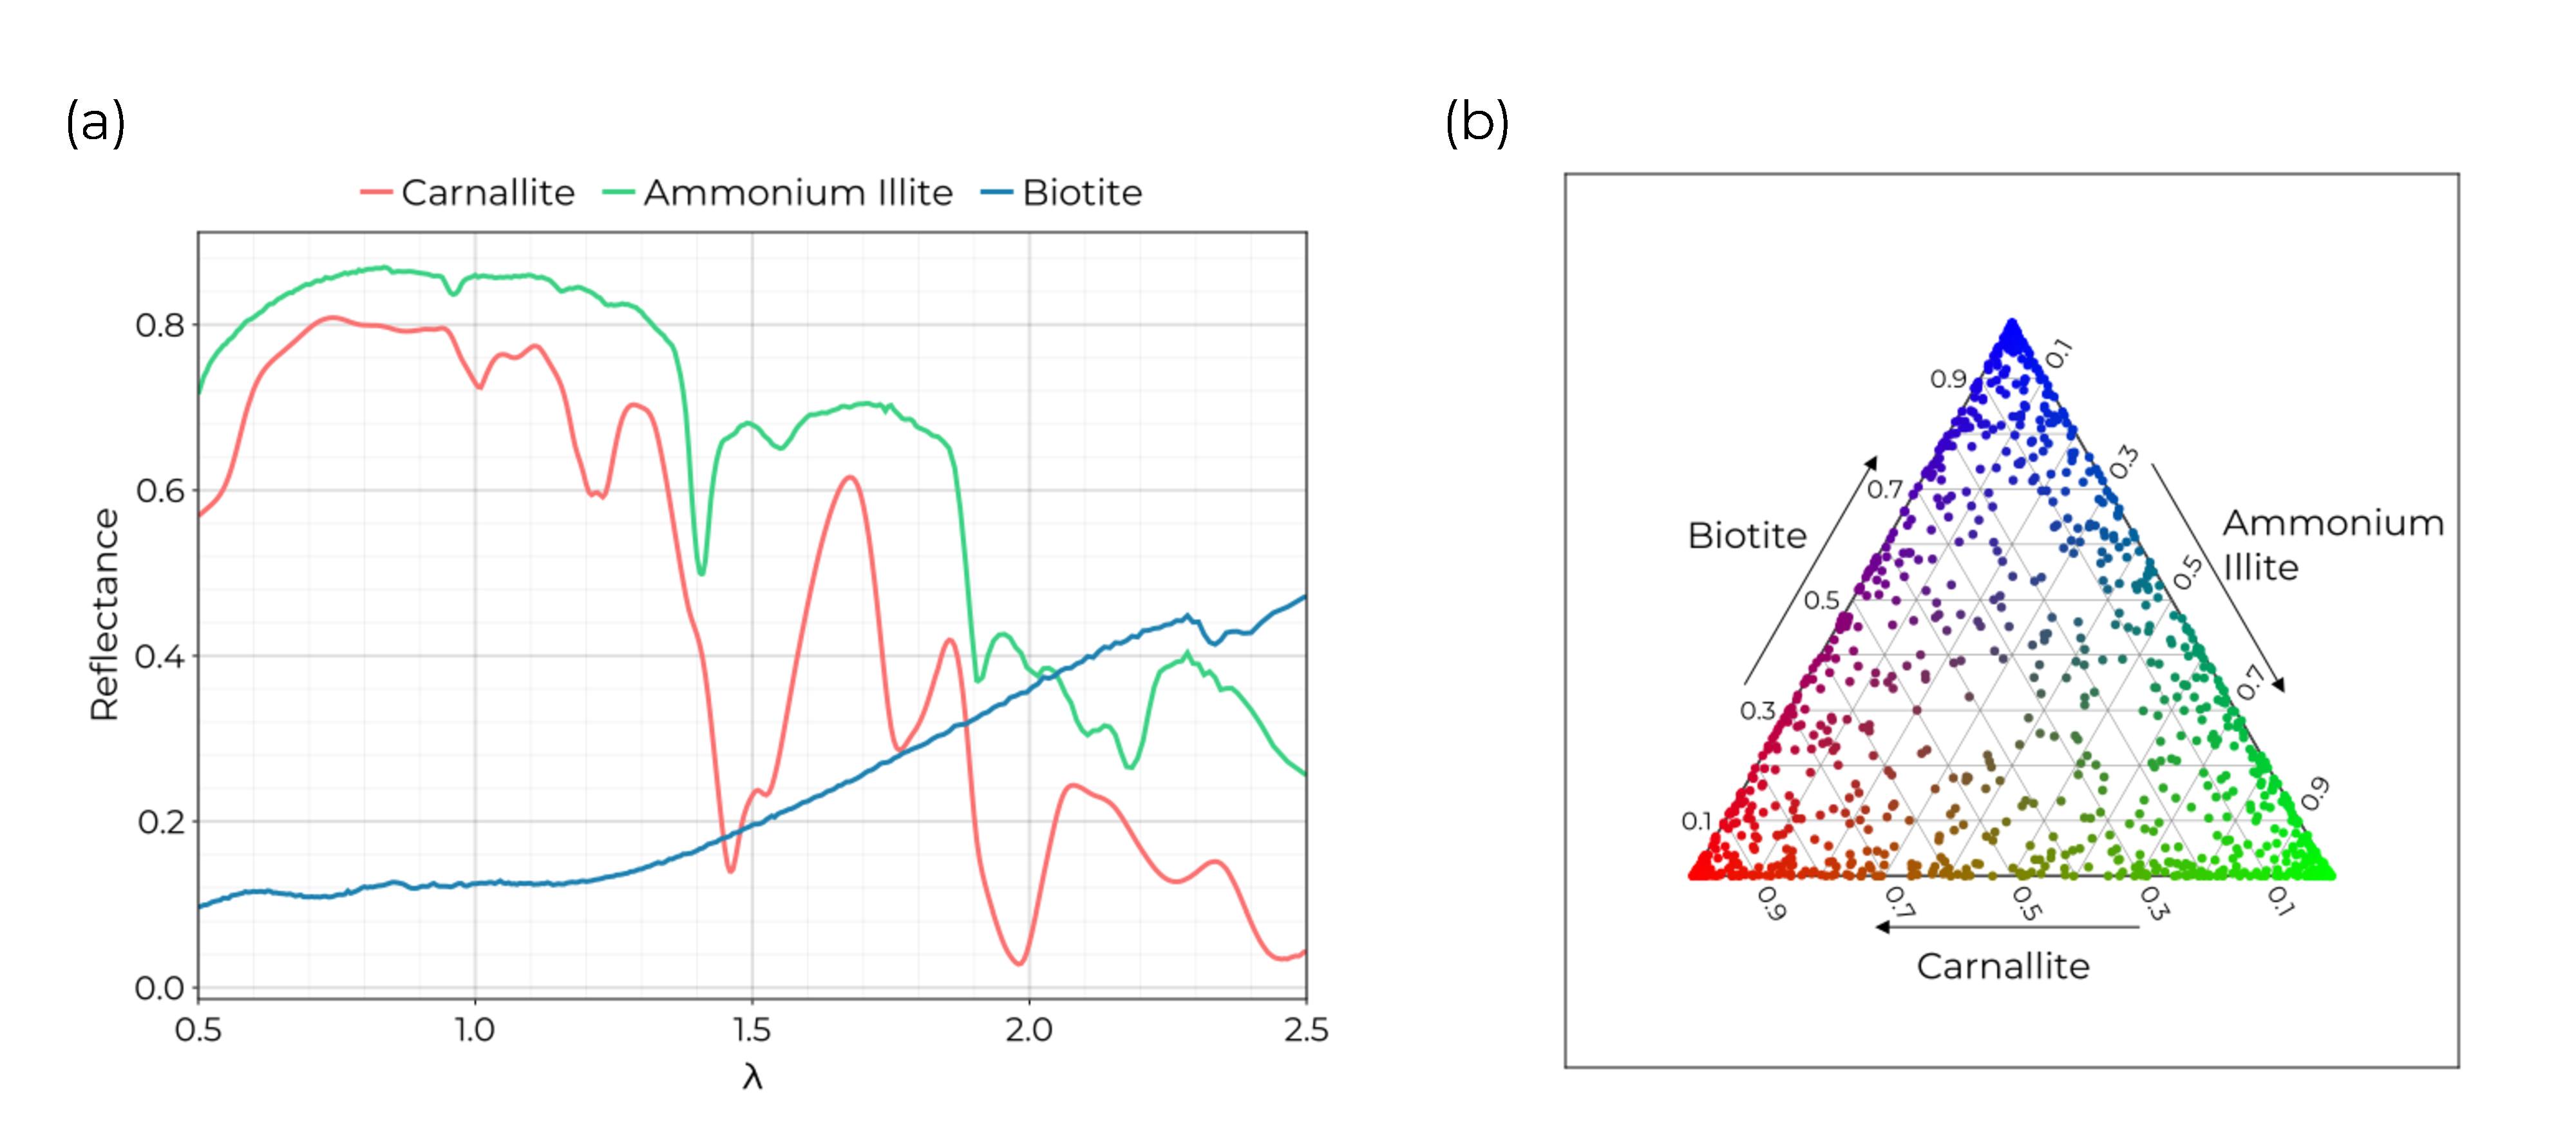
\includegraphics[width=\columnwidth]{robot-team-gsm/methods/usgs/usgs-dataset.pdf}
  \caption{Synthetic data set formed from USGS spectra. \textbf{(a)} Spectra
    from the USGS spectral database used as the ground truth endmembers. These
    spectra were selected following the example in ref. \cite{vca-orig}.
    \textbf{(b)} The abundance distribution sampled for in the data set. Samples
    were generated from a Dirichlet distribution with
    $\alpha_1=\alpha_2=\alpha_3=1/3$.}
  \label{fig:usgs-data}
\end{figure}

Zero-mean Gaussian noise was added to the data to yield $9$ data sets with signal-to-noise ratios (SNR) ranging from $0$ to $\infty$ to examine the impact of random noise on GSM performance. For each of these data sets, a GSM was trained using $25$ nodes per edge with $\lambda_e$ set to the default value of $0.01$ and $\lambda_w$ fixed to $100$. The large value of $\lambda_w$ was chosen to encourage the GSM to prefer models with limited non-linear mixing.

For comparison, NMF models were also trained on each data set as this method is both highly popular and does not include the pure-pixel assumption common to other technqieus like VCA and PPI. Countless variations on the original NMF method have been introduced into the literature with one review identifying more than $100$ distinct NMF variations \cite{unmixing-nmf-review}. For the purpose of evaluating the GSM, we considered the standard $\ell_2$ and KL-divergence formulations introduced by Lee and Seung \cite{nmf-algorithms}. We also included the robust $\ell_{2,1}$ NMF as described by Kong et al \cite{nmf-l21}.

Four metrics were used to compare model performance. For endmember extraction the mean spectral angle and mean RMSE between true endmembers $\rho_i$ and extracted endmembers $\hat{\rho}_i$ were computed where the spectral angle for the $i$-th endmember is defined as
\begin{equation}
    \theta(\rho_i, \hat{\rho}_i) =  \arccos\left( \dfrac{\langle \rho_i, \hat{\rho}_i \rangle}{\lVert \rho_i \rVert \cdot \lVert \hat{\rho}_i \rVert}\right)
\end{equation}
and the RMSE for the $i$-th endmember is
\begin{equation}
    \text{RMSE}(\rho_i, \hat{\rho}_i) = \sqrt{\frac{1}{D-1}\sum_d^D\left(\rho_i(\lambda_d) - \hat{\rho}_i(\lambda_d) \right)^2}.
\end{equation}
Abundance estimation was similarly evaluated using the Mean RMSE between true abundance and estimated abundance values for each endmember. Finally, the reconstruction RMSE, that is, the RMSE computed between the original data set and the data set reconstructed via the extracted endmembers and their associated abundances was computed. This provides a model-agnostic criterion to guarantee that each model sufficiently converged during training.

\subsection{Non-linear Mixing: Water Contaminant Identification}

To assess the ability of the GSM to unmix realistic scenes likely to involve non-linear mixing effects, we consider a data set of real HSI collected in Montague, North Texas on 9 December 2020. A Freefly Alta-X autonomous quadcopter was used as a UAV platform and equipped with a Resonon Pika XC2 visible+near-infrared (VNIR) hyperspectral imager to acquire multiple HSI. Each HSI pixel included 462 wavelength bins ranging from $391$ to $1011$ nm. To evaluate the ability of GSM to identify potential contaminant sources, rhodamine dye, a commonly used tracer in hydrological studies, was released into a pond. Two UAV flights spaced 15 minutes apart were used to capture the evolution of the plume as it dispersed into the surrounding water.

The hyperspectral imager is in a pushbroom configuration so that HSI was captured one scan line at a time. Data from an embedded GPS/INS unit enable direct georectification of captured imagery using the method described in \cite{muller2002program}. Additionally, an upward-facing Ocean Optics UV-Vis NIR spectrometer with a cosine corrector was included on the top of the UAV to measure incident solar irradiance. The configuration of the UAV together with a sample HSI are shown in Figure~\ref{fig:robotteam-data}. For a more detailed description of the system, the reader is directed to ref. \cite{robot-team-1, robot-team-2}.

\begin{figure}[H]
  \centering
  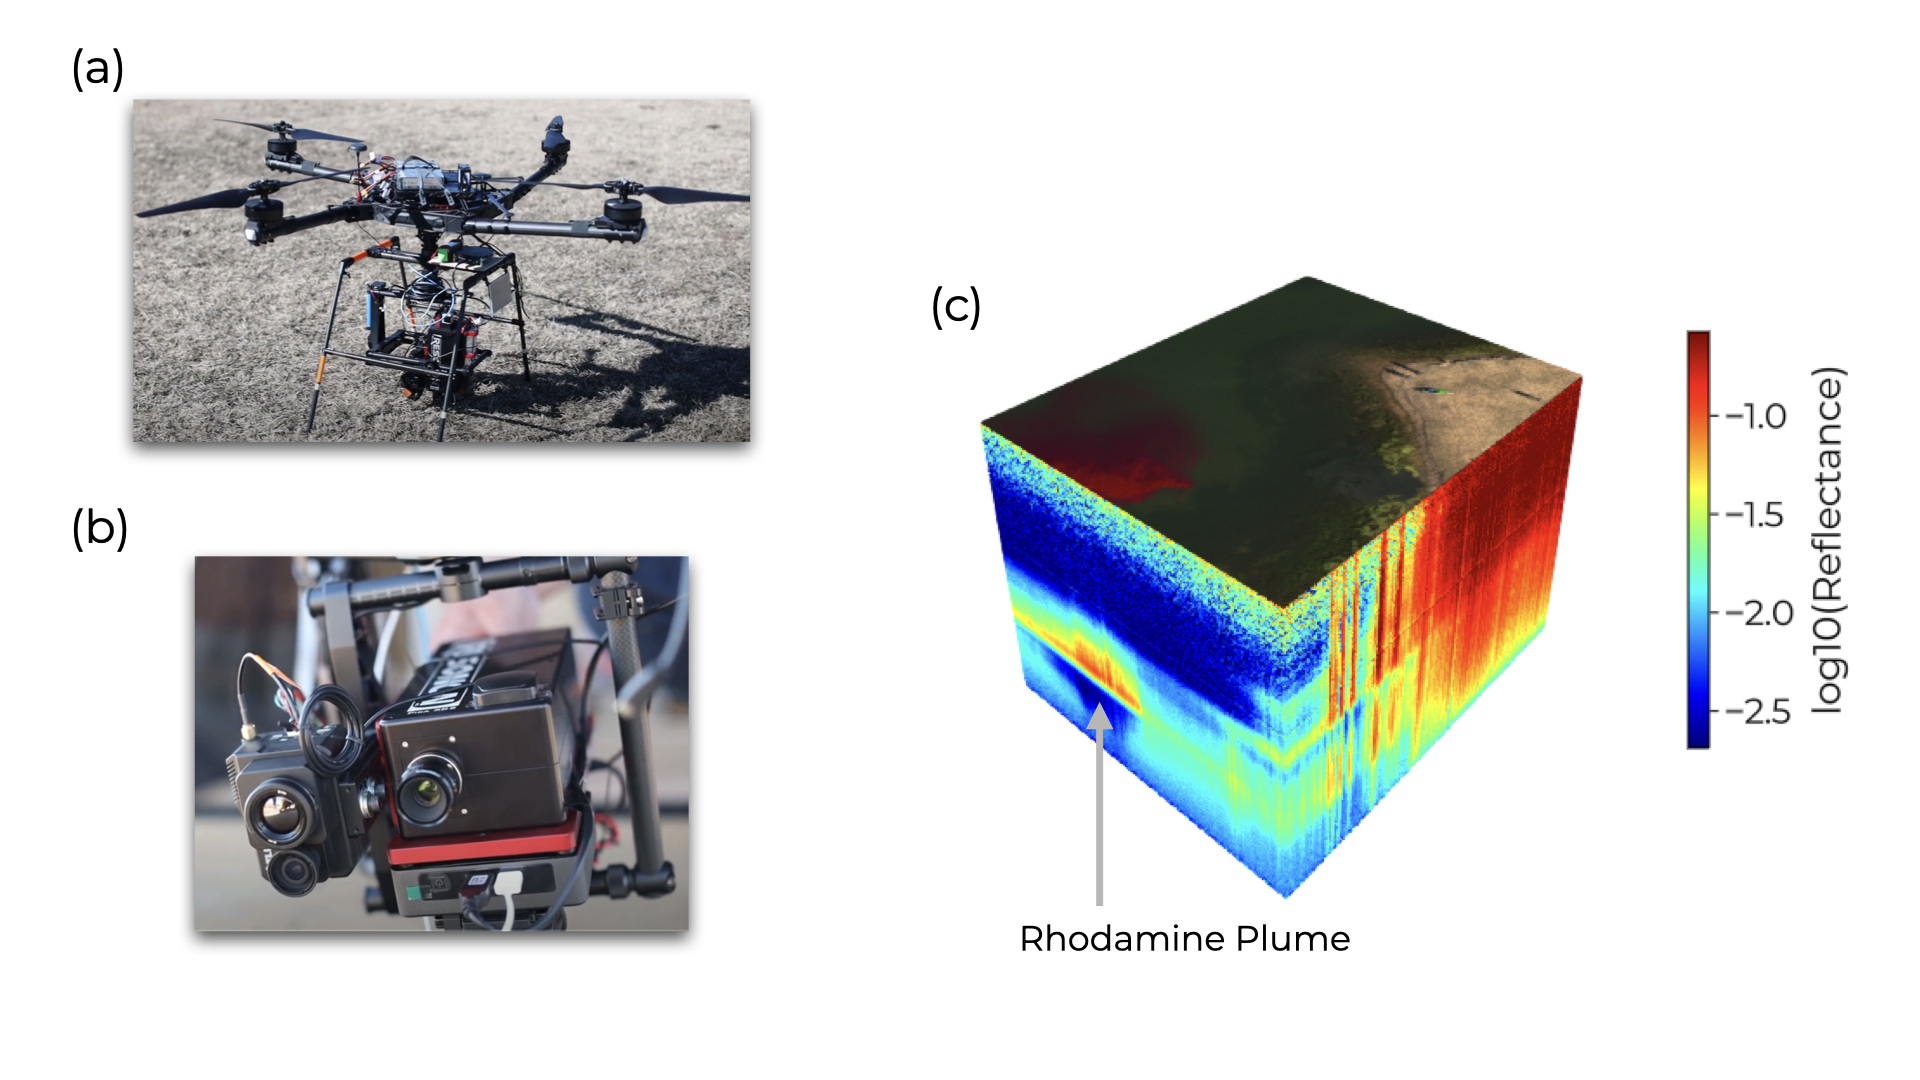
\includegraphics[width=0.9\columnwidth]{robot-team-gsm/methods/robot-team/robot-team-overview.png}
  \caption{Real HSI Data set. \textbf{(a)} the UAV used to collect hyperspectral
    images. \textbf{(b)} The Resonon Pika XC2 hyperspectral imager used to
    acquire HSI. \textbf{(c)} A sample hyperspectral data cube. Spectra a
    plotted using at their geographic position with the log10-reflectance
    colored along the z axis and a pseudocolor image on top. The signature of
    the rhodamine dye plume is clearly identifiable in the
    water.}
  \label{fig:robotteam-data}
\end{figure}

Raw HSI were converted to reflectance using the downwelling irradiance spectrum captured simultaneously with each HSI. Given the UAV flies with the imager oriented to nadir, the reflectance is then given by
\begin{equation}
    \rho(\lambda) = \pi\,L(\lambda)/E_d(\lambda)
\end{equation}
where $L$ is the spectral radiance, $E_d$ is the downwelling irradiance, and a factor of $\pi$ is included resulting from the assumption of diffuse upwelling radiance \cite{ruddick2019review}. The UAV flights were performed near solar noon to maximize the amount of sunlight illuminating the water. For this pond in North Texas, this corresponded to an average solar zenith angle of $56.7^{\circ}$ resulting in HSI with negligible sunglint effects.

From the collected HSI, a water-only pixel mask was generated by identifying all pixel spectra with a normalized difference water index (NDWI) greater than $0.25$ as defined in ref. \cite{ndwi}. Of these water pixels, a combined data set of $15,000$ spectra was sampled for GSM training. As a final processing step, reflectance spectra were limited to $\lambda \leq 900$ nm as wavelengths above this threshold showed significant noise.

In order to justify values for the appropriate number of endmembers, the final data set was decomposed using principal component analysis (PCA). A plot of the explained variance organized for each PCA component is shown in Figure~\ref{fig:robot-team-pca}

The PCA decomposition of the data suggests that at least $3$ endmembers should be used for a mixing model and beyond $6$ there is little added benefit. Based on these observations, multiple GSM models were trained with $N_v$ ranging from $3$ to $6$, $\lambda_e$ ranging from $0.001$ to $1.0$, and $\lambda_w$ ranging from $1$ to $1000$ in order to explore the GSM parameter space. From these, a final model was identified using the BIC, AIC, and reconstruction RMSE. The resulting GSM was then explored to examine extracted endmembers and map the evolution of the rhodamaine plume by using the abundances given by the latent space representation of each pixel in the HSI.

\begin{figure}[H]
  \centering
  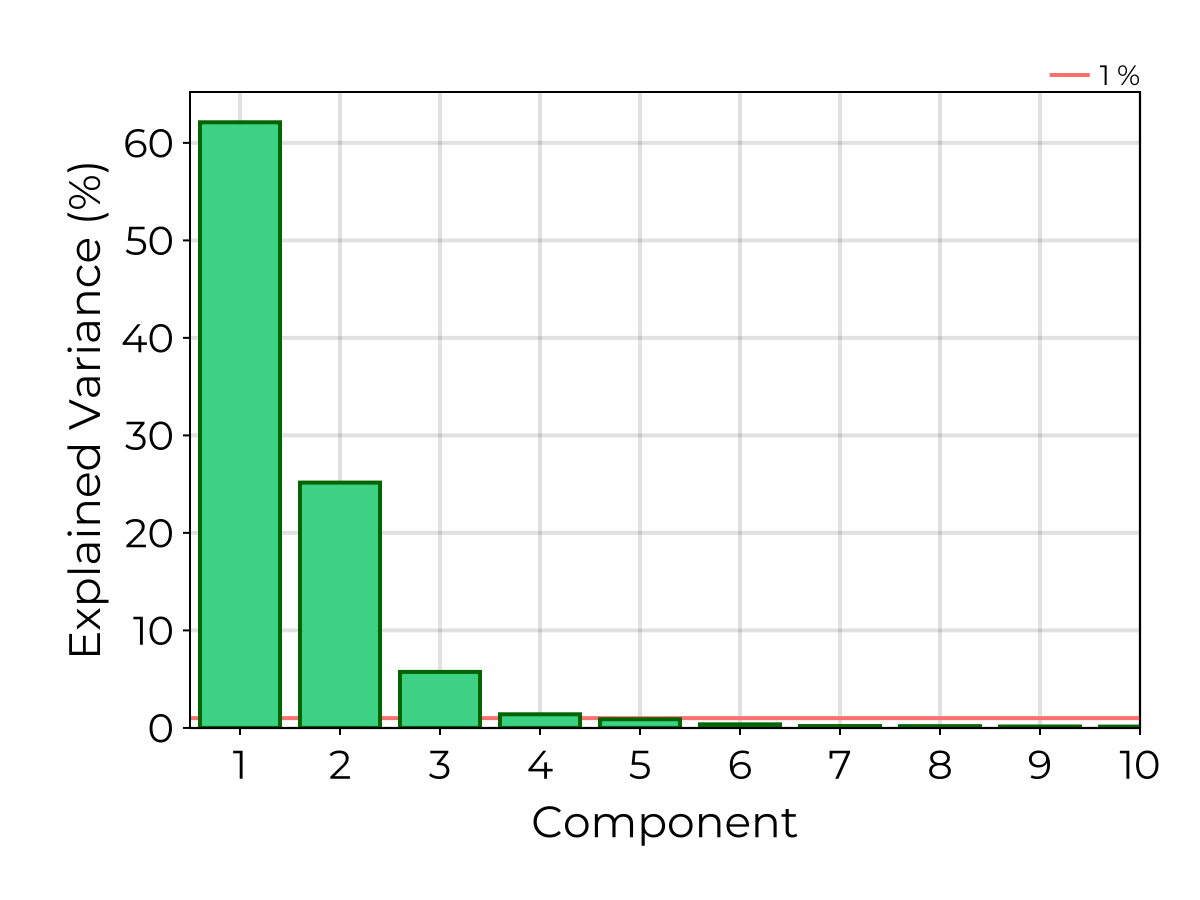
\includegraphics[width=0.60\columnwidth]{robot-team-gsm/results/robot-team/pca-variance.png}
  \caption{Explained variance of PCA components for the real HSI data set. A red
    horizontal line is superimposed on the graph, marking an explained variance
    of $1\%$. All components past the fourth explain less than $1\%$ of the
    observed variance.}
  \label{fig:robot-team-pca}
\end{figure}






\section{Results}


\subsection{Linear Mixing}

The results of GSM training on the synthetic linear mixing data set described in Sec~\ref{sec:experiments} are illustrated in Figure~\ref{fig:usgs-fits}. Three versions of NMF were trained corresponding to Euclidean ($\ell_2$), KL-Divergence, and $\ell_{2,1}$ cost functions. GSM models using both a regular simplex grid and a grid of points sampled using a uniform Dirichlet distribution (referred to as a \textit{big} GSM model) were trained to compare performance in linear mixing tasks.

\newpage

\begin{figure}[H]
  \centering
  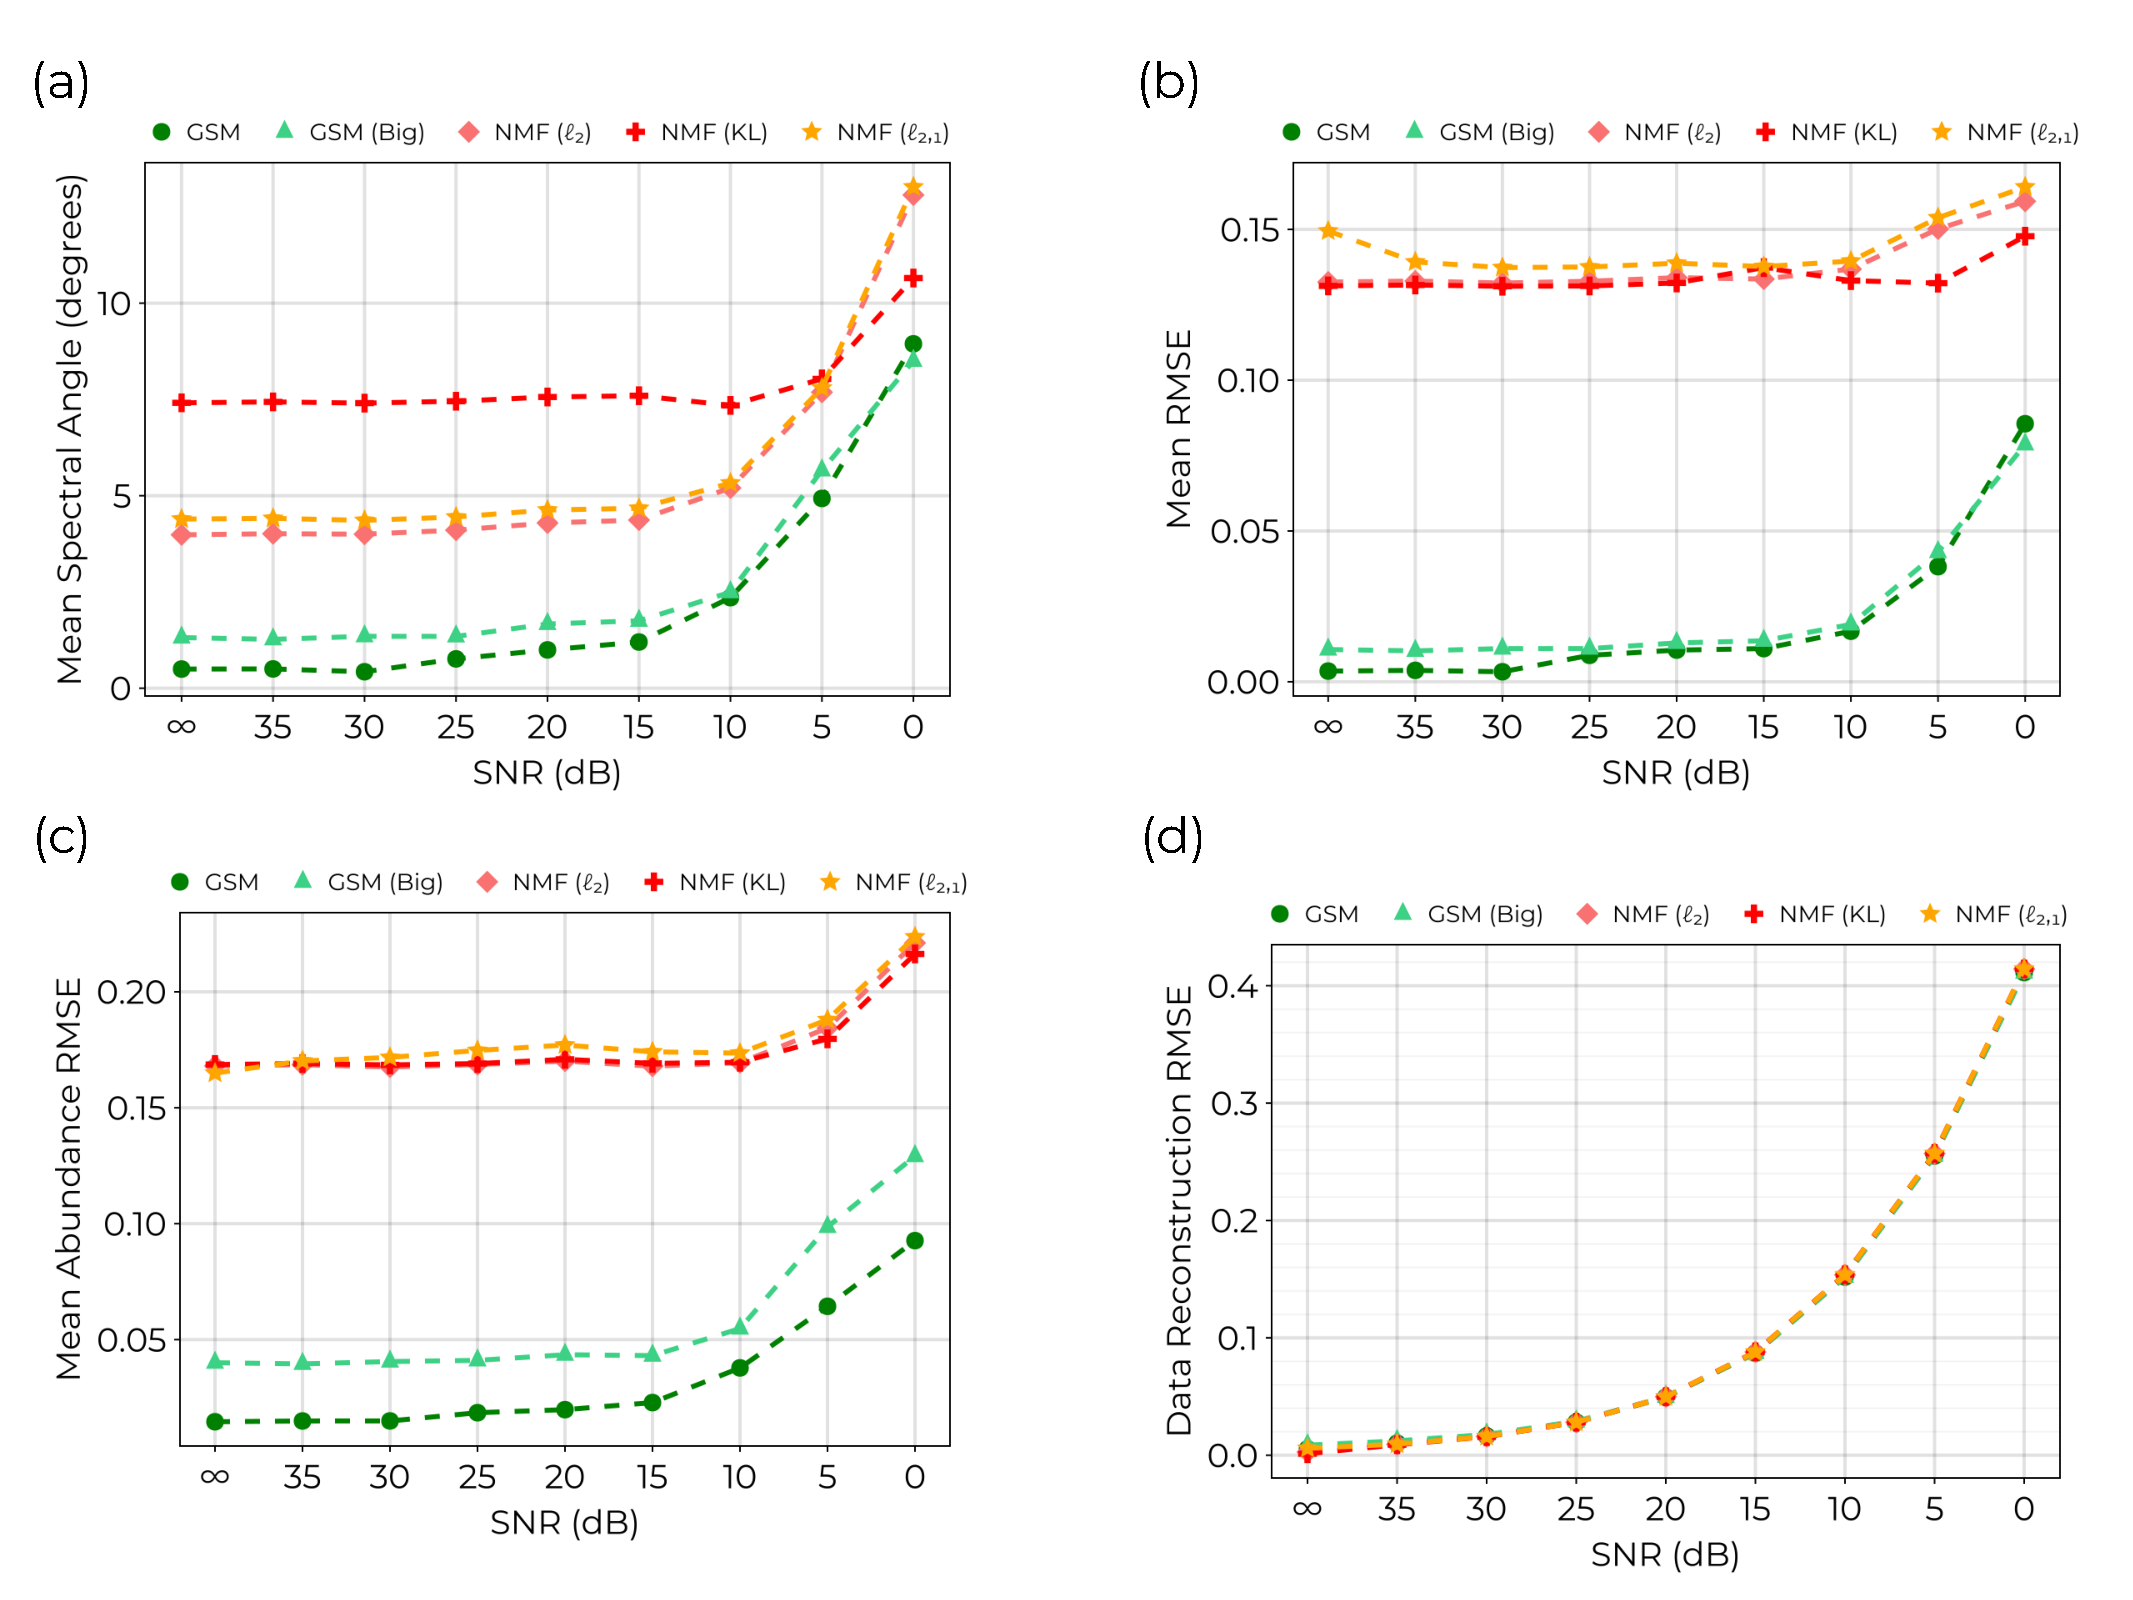
\includegraphics[width=\columnwidth]{robot-team-gsm/results/usgs/fit-comparison.pdf}
  \caption{Comparison of GSM against NMF on simulated linear mixing data set
    using USGS spectra. \textbf{(a)} The mean spectral angle computed between
    extracted endmembers and original endmembers. \textbf{(b)} the mean RMSE
    computed between extracted endmembers and original endmembers. \textbf{(c)}
    The mean abundance RMSE computed between original abundance data for each
    endmember and extracted abundances. \textbf{(d)} The reconstruction RMSE
    which evaluates the quality of fit. All models realized similar values
    reflecting convergence of the models to the level of random noise introduced
    into the data.}
  \label{fig:usgs-fits}
\end{figure}

The quality of endmember extraction is measured by the mean spectral angle and the mean endmember RMSE. As Figure~\ref{fig:usgs-fits} indicates, both versions of the GSM outperformed their NMF counterparts. Additionally, we note that for all GSM models, even including $\text{SNR}=0$, all model weights $W_{dm}$ for $m>N_v$ corresponding to non-linear mixing were driven identically to $0.0$. This confirms that, for data sets with purely linear mixing and random noise, the GSM correctly fits a mixing model without introducing unnecessary complexity.

The quality of the unmixing, that is, the estimation of the abundance, performed by each model was evaluated using the mean abundance RMSE. Here we again see that both versions of the GSM outperformed NMF. To justify that all models were fairly trained to convergence, the RMSE data reconstruction was also computed. This metric uses the trained mixing model to compute the error between the original data set and the reconstructed spectra generated using the extracted endmembers and their abundances. For all GSM and NMF models, the RMSE data reconstruction converged to the level of random noise introduced into the data. These results reflect a fair comparison between the NMF and GSM models.

In Figure~\ref{fig:usgs-endmembers}, we plot the endmembers extracted for the GSM model trained on the synthetic data set with $\text{SNR}=20$.

\begin{figure}[H]
  \centering
  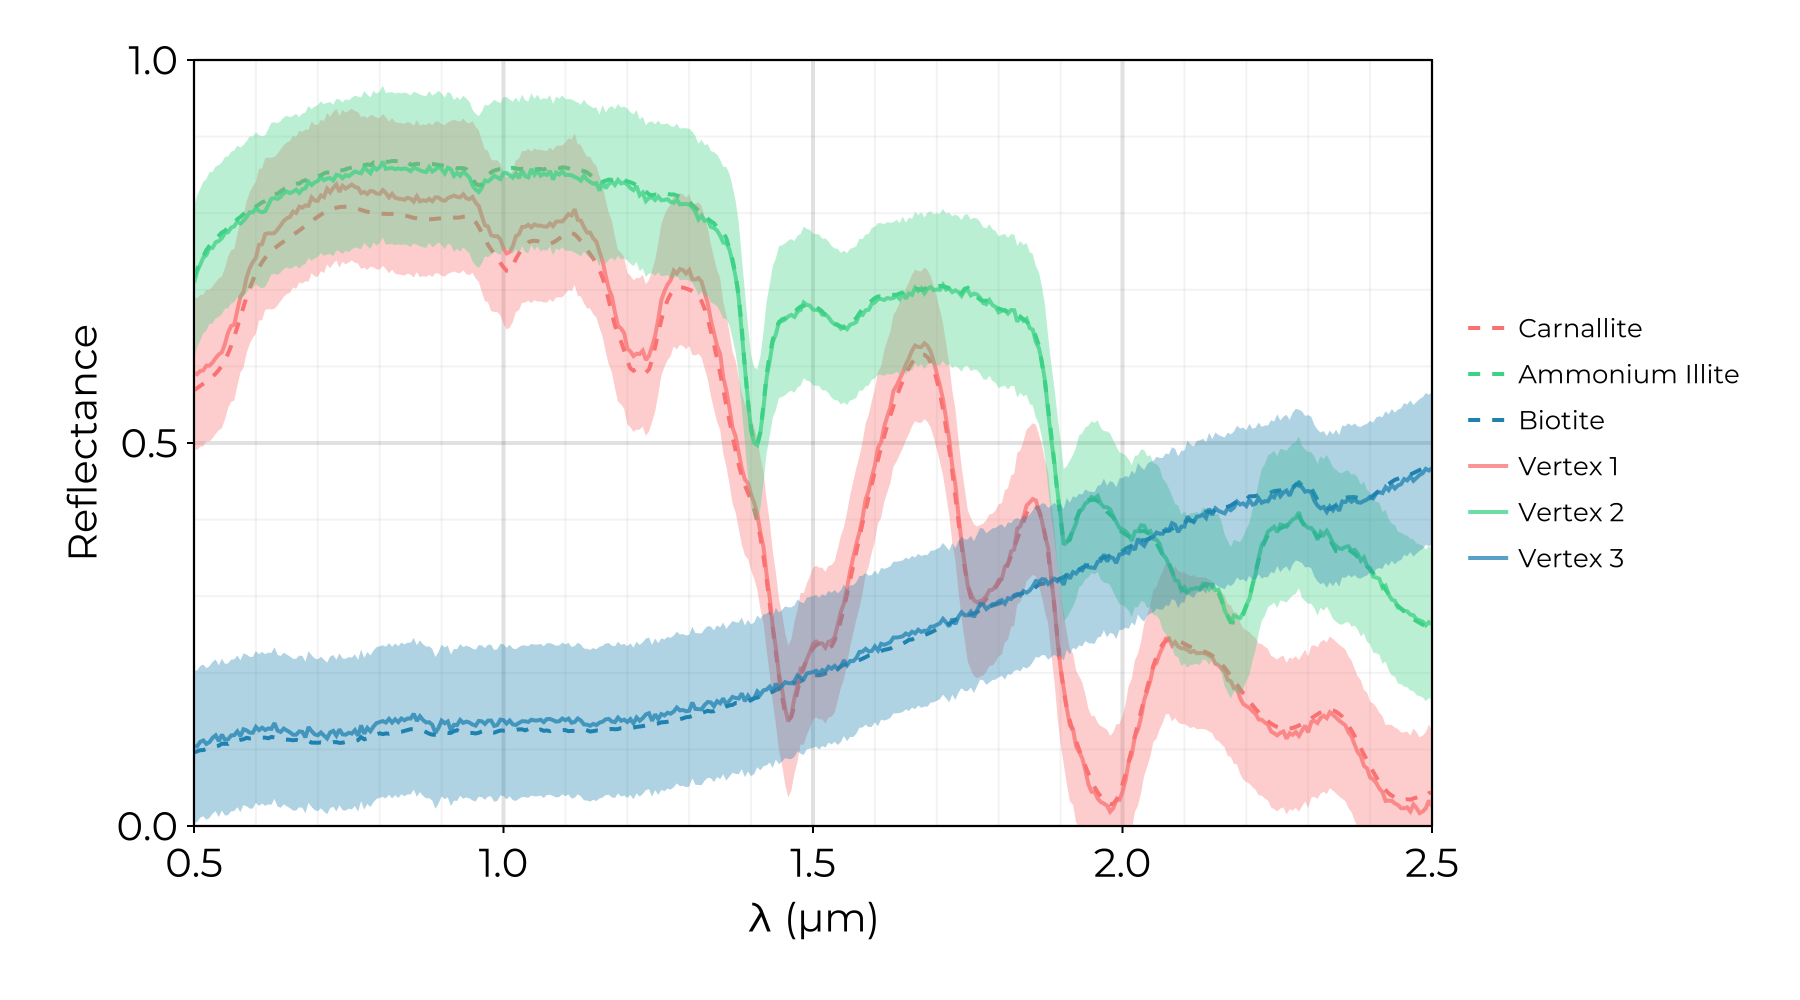
\includegraphics[width=\columnwidth]{robot-team-gsm/results/usgs/extracted-endmembers.png}
  \caption{Endmembers extracted by the GSM for the simulated linear mixing data
    set with SNR$=20$. The dashed lines correspond to original endmember spectra
    from the USGS spectral database. Solid lines superimposed on the plot
    indicate the extracted endmember spectra. Colored bands are included around
    each spectrum corresponding to the spectral variability estimated by the GSM
    precision parameter $\beta$ where the band width is $2\sqrt{\beta^{-1}}$
    corresponding to $2$ standard deviations.}
  \label{fig:usgs-endmembers}
\end{figure}

The extracted endmembers clearly fit the original source spectra while capturing local reflectance features. Furthermore, the GSM precision parameter $\beta$ which is tuned during model training, provides an assessment of spectral variability due to random noise. In Figure~\ref{fig:usgs-endmembers} this is indicated by the colored band centered around each extracted spectrum with a width of $2\sqrt{\beta^{-1}}$ corresponding to 2 standard deviations. The SNR of $20$ added to this example corresponds to zero-mean Gaussian noise with a standard deviation of $\sigma=0.0493$. After training, the GSM found $\sqrt{\beta^{-1}}=0.0495$ that accurately captures the introduced noise. This ability to assess the spectral variability of extracted endmembers is a key advantage of the GSM.

\subsection{Non-linear Mixing: Rhodamine Dye Plume}

For the data set of real HSI spectra described in Section~\ref{sec:experiments},
80 GSM models were trained to explore the GSM hyperparameter space. The
performance of the model was compared using the BIC, AIC and RMSE reconstruction
with the results of the top $10$ performing models shown in
Table~\ref{table:fit-comparison}.

\begin{table}[H]
  \caption{GSM hyperparameter optimization for the real HSI data set: Multiple
    GSM models were trained to explore the impact of model hyperparameters.
    $N_v$ values from $3$ to $6$ were explored as suggested by the PCA
    decomposition of the data set. $\lambda_e$ was varied from $0.001$ to $1.0$
    and $\lambda_w$ ranged from $1$ to $1000$. Here we report the top $10$
    models ranked by increasing BIC. The AIC and reconstruction RMSE are also
    included for comparison.}
  \label{table:fit-comparison}
  \begin{center}
  \begin{tabular}{cccccc} \hline
    \textbf{$N_v$}	& \textbf{$\lambda_e$}	& \textbf{$\lambda_w$} &
    \textbf{BIC} & \textbf{AIC} & \textbf{Reconstruction RMSE}\\ \hline
    $3$ & $0.01$    & $1.0$     & $-6.195\times10^7$   & $-6.269\times10^7$   & $0.000989$ \\
    $3$	& $0.001$   & $1.0$     & $-6.194\times10^7$   & $-6.268\times10^7$   & $0.000989$ \\
    $3$	& $0.1$     & $1.0$	    & $-6.192\times10^7$   & $-6.265\times10^7$   & $0.000991$ \\
    $3$	& $1.0$     & $1.0$	    & $-6.186\times10^7$   & $-6.260\times10^7$   & $0.001190$ \\
    $4$	& $1.0$     & $1.0$	    & $-6.181\times10^7$   & $-6.255\times10^7$   & $0.001002$ \\
    $4$	& $0.1$     & $1.0$	    & $-6.175\times10^7$   & $-6.249\times10^7$   & $0.001008$ \\
    $4$	& $0.01$    & $1.0$     & $-6.173\times10^7$   & $-6.247\times10^7$   & $0.001009$ \\
    $4$	& $0.001$   & $1.0$     & $-6.173\times10^7$   & $-6.247\times10^7$   & $0.001009$ \\
    $4$	& $0.1$     & $10.0$    & $-6.171\times10^7$   & $-6.245\times10^7$   & $0.001011$ \\
    $3$	& $1.0$     & $10.0$    & $-6.166\times10^7$   & $-6.239\times10^7$   & $0.001014$
  \end{tabular}
  \end{center}
\end{table}

As the table indicates, a non-linear GSM with $N_v=3$, $\lambda_e=0.01$, and $\lambda_w=1.0$ achieved minimum BIC, AIC, and reconstruction RMSE values. The lower value of $\lambda_w$ identified from these models reflects the presence of non-linear mixing effects in the HSI data. Although the values of model weights $W_{dm}$ for $m>N_v$ corresponding to non-linear mixing were $0$ for the synthetic data set, here these weights obtained a small but non-negligible median value of $0.0012$.

Reflectance spectra generated by the trained GSM corresponding to the maximum abundance values for each endmember are plotted in Figure~\ref{fig:robot-team-endmembers}. Based on their signatures, these endmembers are identified with water, vegetation (including near shore, filamentous blue-green algae) and the rhodmaine dye plume.

\begin{figure}[H]
  \centering
  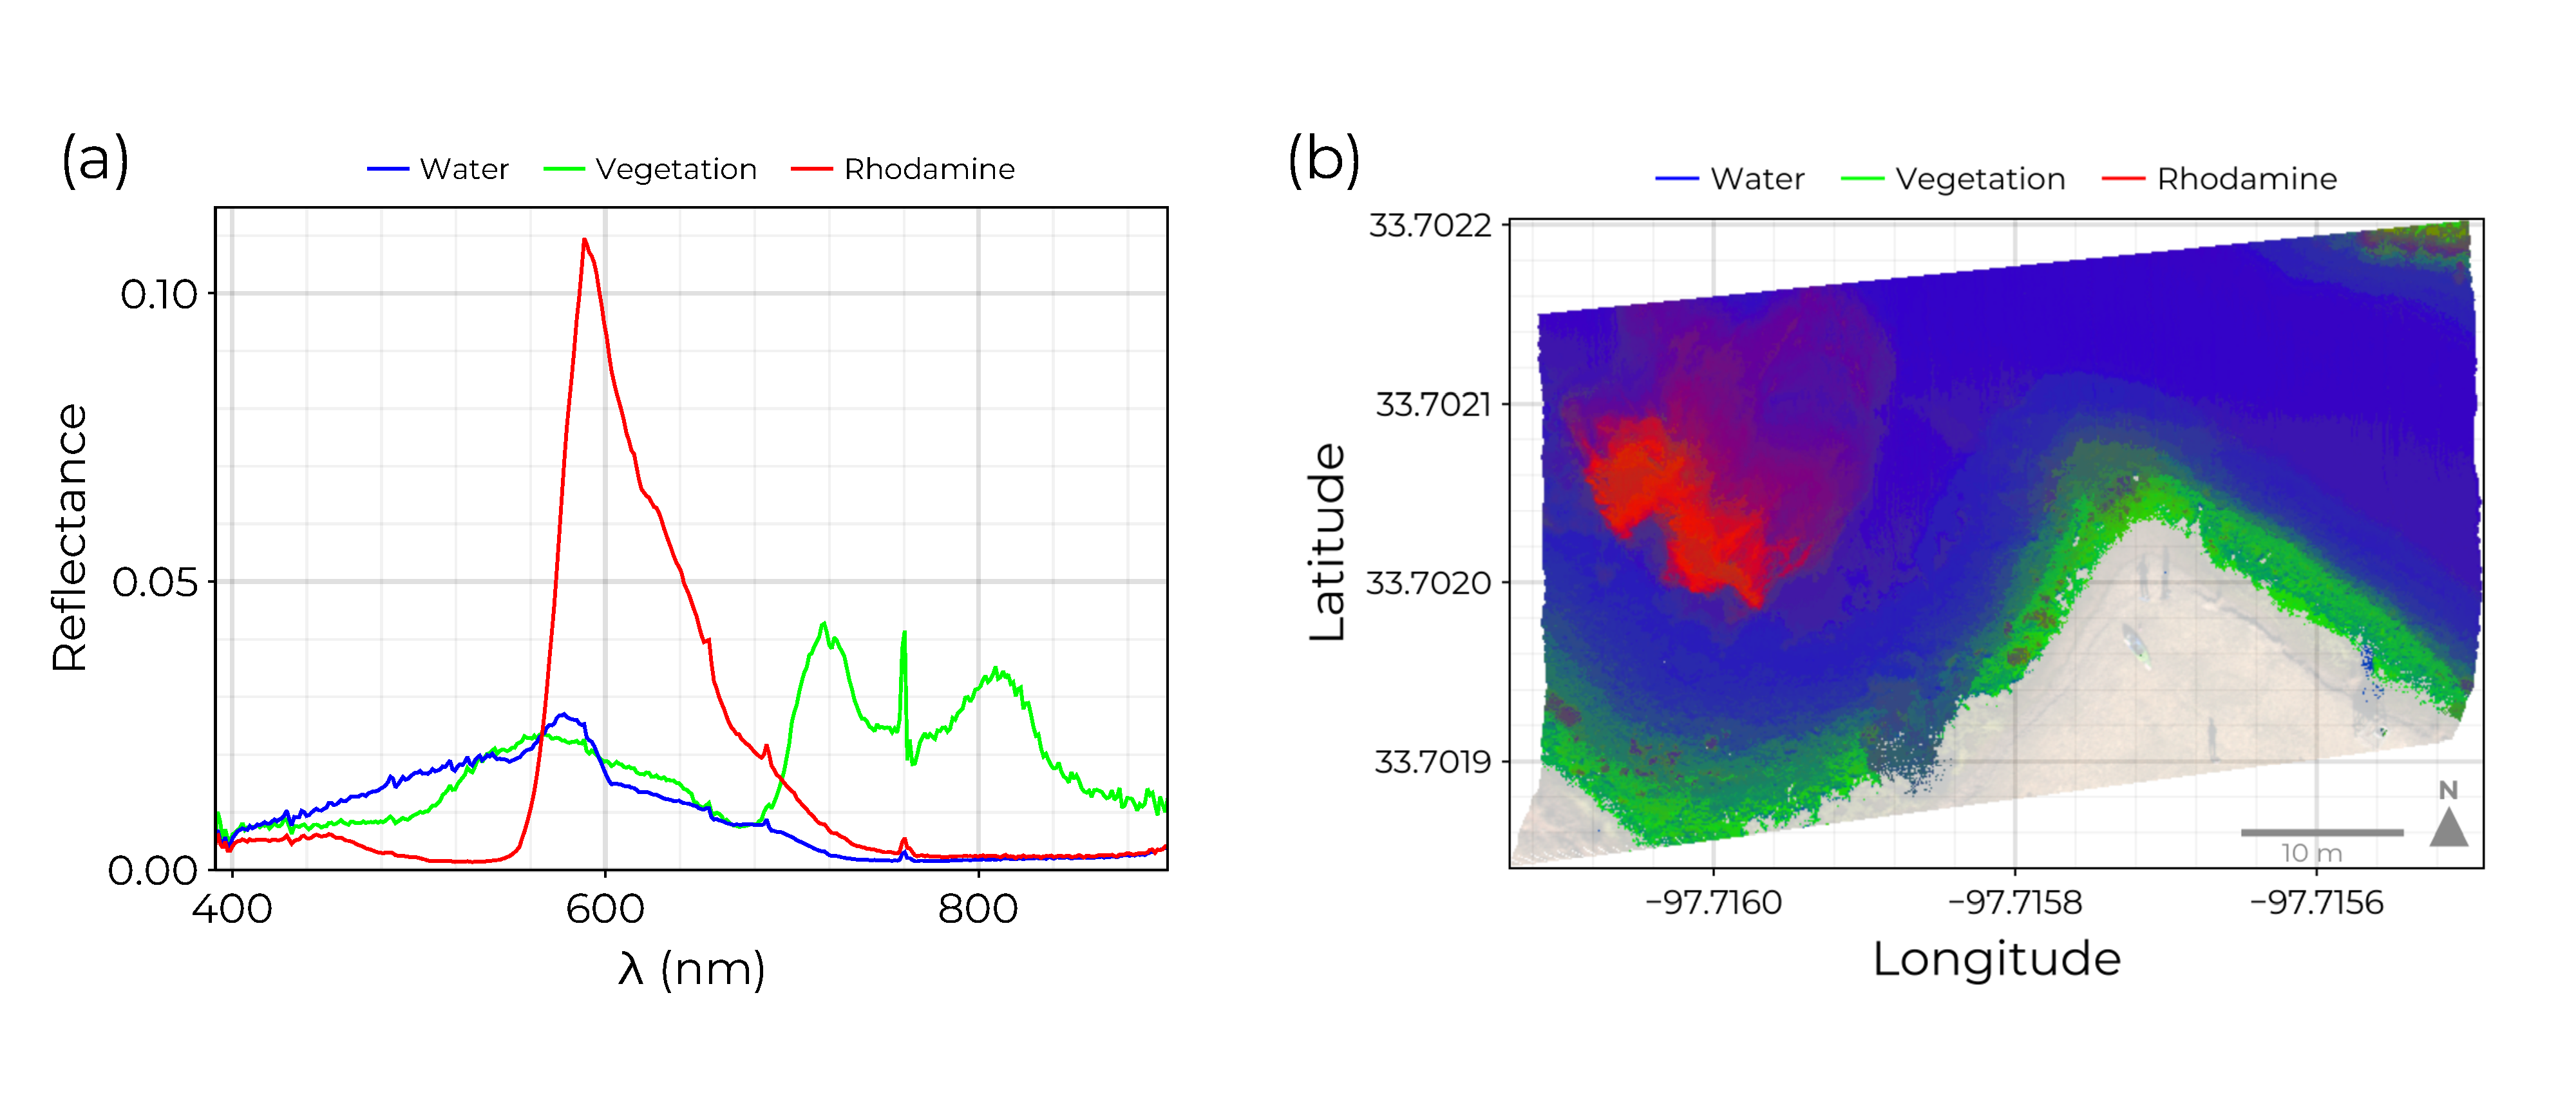
\includegraphics[width=\columnwidth]{robot-team-gsm/results/robot-team/extracted-endmembers.pdf}
  \caption{GSM applied to water spectra from real HSI data set: \textbf{(a)}
    Spectra generated by the trained GSM for samples with maximum abundance for
    each endmember. Based on these spectral profiles, endmembers are identified
    with water, near-shore vegetation, and rhodamine dye. \textbf{(b)} A HSI
    segmented according to the relative abundance of each endmember. Each water
    pixel is colored by smoothing interpolating between red, green, and blue
    colors using the relative abundance estimated for rhodamine, vegetation, and
    water spectra. The rhodamine plume is clearly identifiable in the western
    portion of the HSI.}
  \label{fig:robot-team-endmembers}
\end{figure}



% \clearpage
% \newpage

% \begin{sidewaysfigure}
%   \centering
%   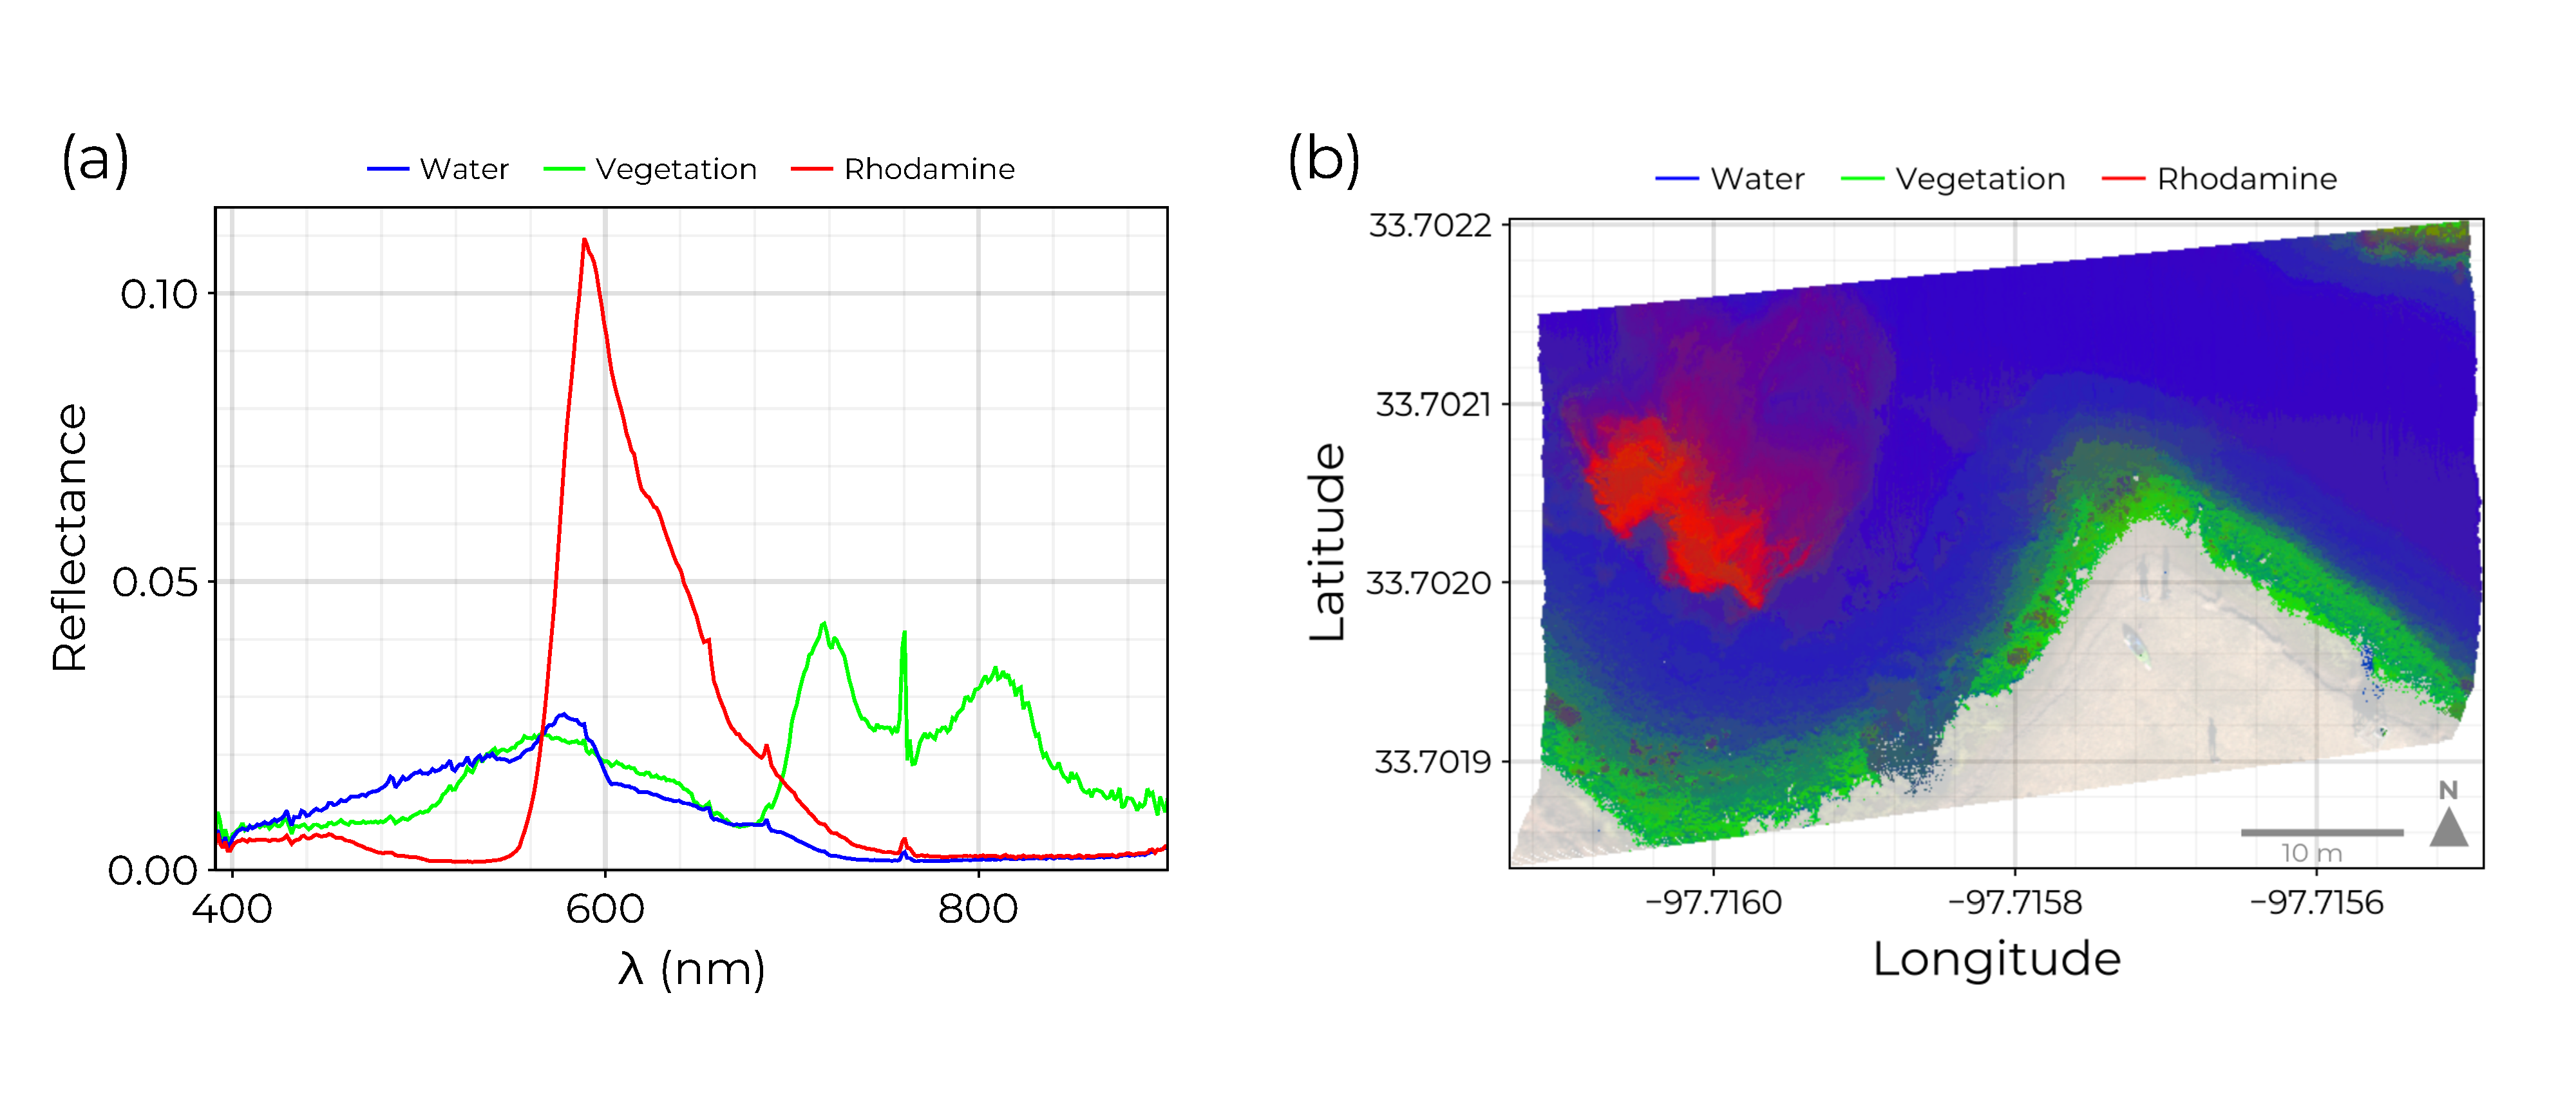
\includegraphics[width=\columnwidth]{robot-team-gsm/results/robot-team/extracted-endmembers.pdf}
%   \caption{GSM applied to water spectra from real HSI data set: \textbf{(a)}
%     Spectra generated by the trained GSM for samples with maximum abundance for
%     each endmember. Based on these spectral profiles, endmembers are identified
%     with water, near-shore vegetation, and rhodamine dye. \textbf{(b)} A HSI
%     segmented according to the relative abundance of each endmember. Each water
%     pixel is colored by smoothing interpolating between red, green, and blue
%     colors using the relative abundance estimated for rhodamine, vegetation, and
%     water spectra. The rhodamine plume is clearly identifiable in the western
%     portion of the HSI.}
%   \label{fig:robot-team-endmembers}
% \end{sidewaysfigure}

% \clearpage
% \newpage

By assigning a unique color to each endmember, the spatial distribution of HSI spectra can be visualized by using estimated abundances to smoothly interpolate between endmember colors as shown in panel b of Figure~\ref{fig:robot-team-endmembers}. In other words, this method provides a fuzzy semantic segmentation of HSI pixels. Alternatively, each HSI pixel could be assigned a single class corresponding to the endmember with maximal abundance. In this way, the GSM can be used to visualize high-dimensional HSI spectra.

To showcase the ability of the GSM to identify spatially localized contaminant sources, abundance maps were generated for each individual end member using the trained GTM to unmix all water pixels in the HSI. In Figure~\ref{fig:endmember-abundance-dist} these abundance maps are compared for each endmember. The abundance map for the water endmember covers a majority of the center of the pond and decreases near the edge of the rhodamine plume where the dye and water mix. The vegetation in shallow water near the shore and the rhodamine dye plume in the western half of the pond are also clearly identified by their abundance maps. Given an HSI pixel resolution of $0.1 \times 0.1$ $\text{m}^2$, the spatial extent of vegetation is estimated to be $378.6$ $\text{m}^2$ while the plume initially extends across $255.7$ $\text{m}^2$.

\newpage

\begin{figure}[H]
  \vspace{-1.5cm}
  \centering
  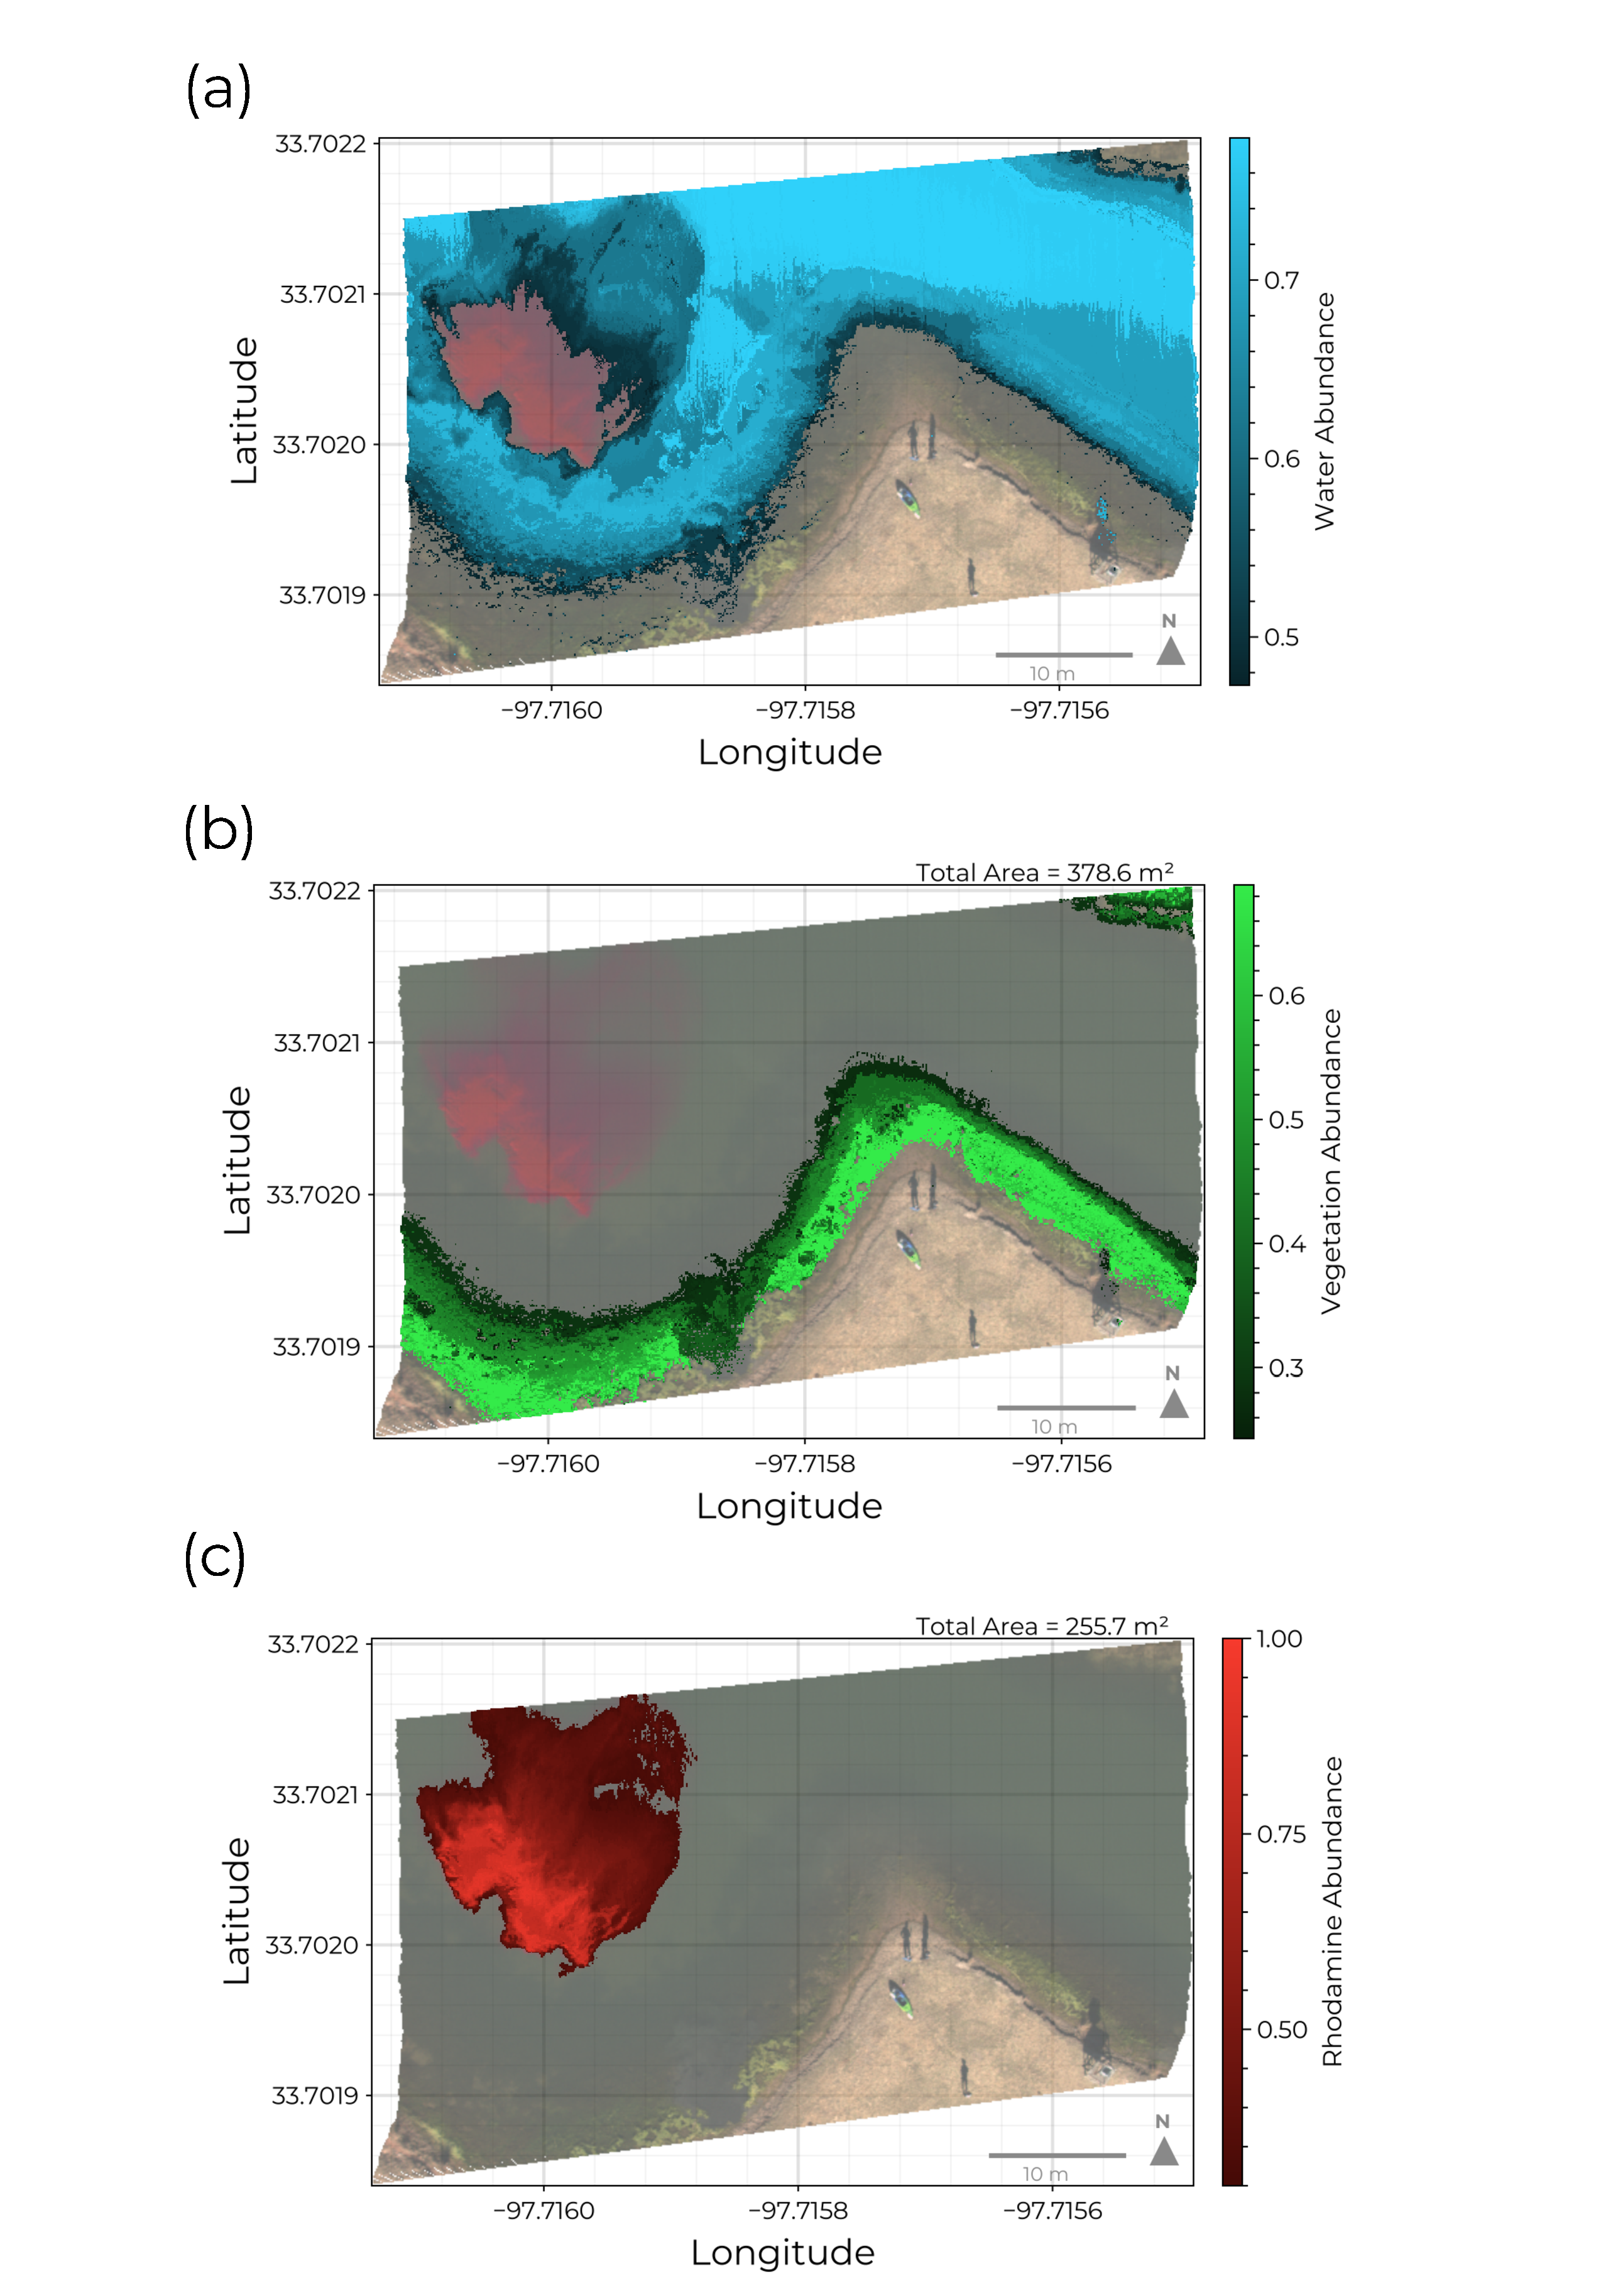
\includegraphics[width= 0.8\columnwidth]{robot-team-gsm/results/robot-team/endmember-abundances.pdf}
  \caption{Endmember abundance distributions: \textbf{(a)} The spatial
    distribution of abundance for the water class. This source dominates in the
    center of the pond and decreases towards the shore where vegetation begins
    to dominate the reflectance signal. The water endmember abundance is also
    observed to decreases near the edge of the rhodamine plume reflecting dye
    mixing and diffusion. \textbf{(b)} The spatial distribution of vegetation.
    This endmember includes filamentous blue-green algae observed to accumulate
    in shallow waters near the shore. \textbf{(c)} The rhodamine dye plume
    extent segmented from the HSI. The total area for near-shore vegetation and
    rhodamine are estimated to be $378.6$ $\text{m}^2$ and $255.7$ $\text{m}^2$,
    respectively.}
  \label{fig:endmember-abundance-dist}
\end{figure}


Applying the trained GSM to unmix HSI from UAV flights provides an efficient way to map the dispersion and transport of contaminant. Figure~\ref{fig:plume-evo} demonstrates this by mapping the growing extent of rhodamine dye between successive UAV flights. In just $15$ minutes, the plume expands from an initial area of $255.7$ $\text{m}^2$ to over $571.8$ $\text{m}^2$ as the dye mixes with the surrounding water.

\clearpage
\newpage

\begin{sidewaysfigure}
  \centering
  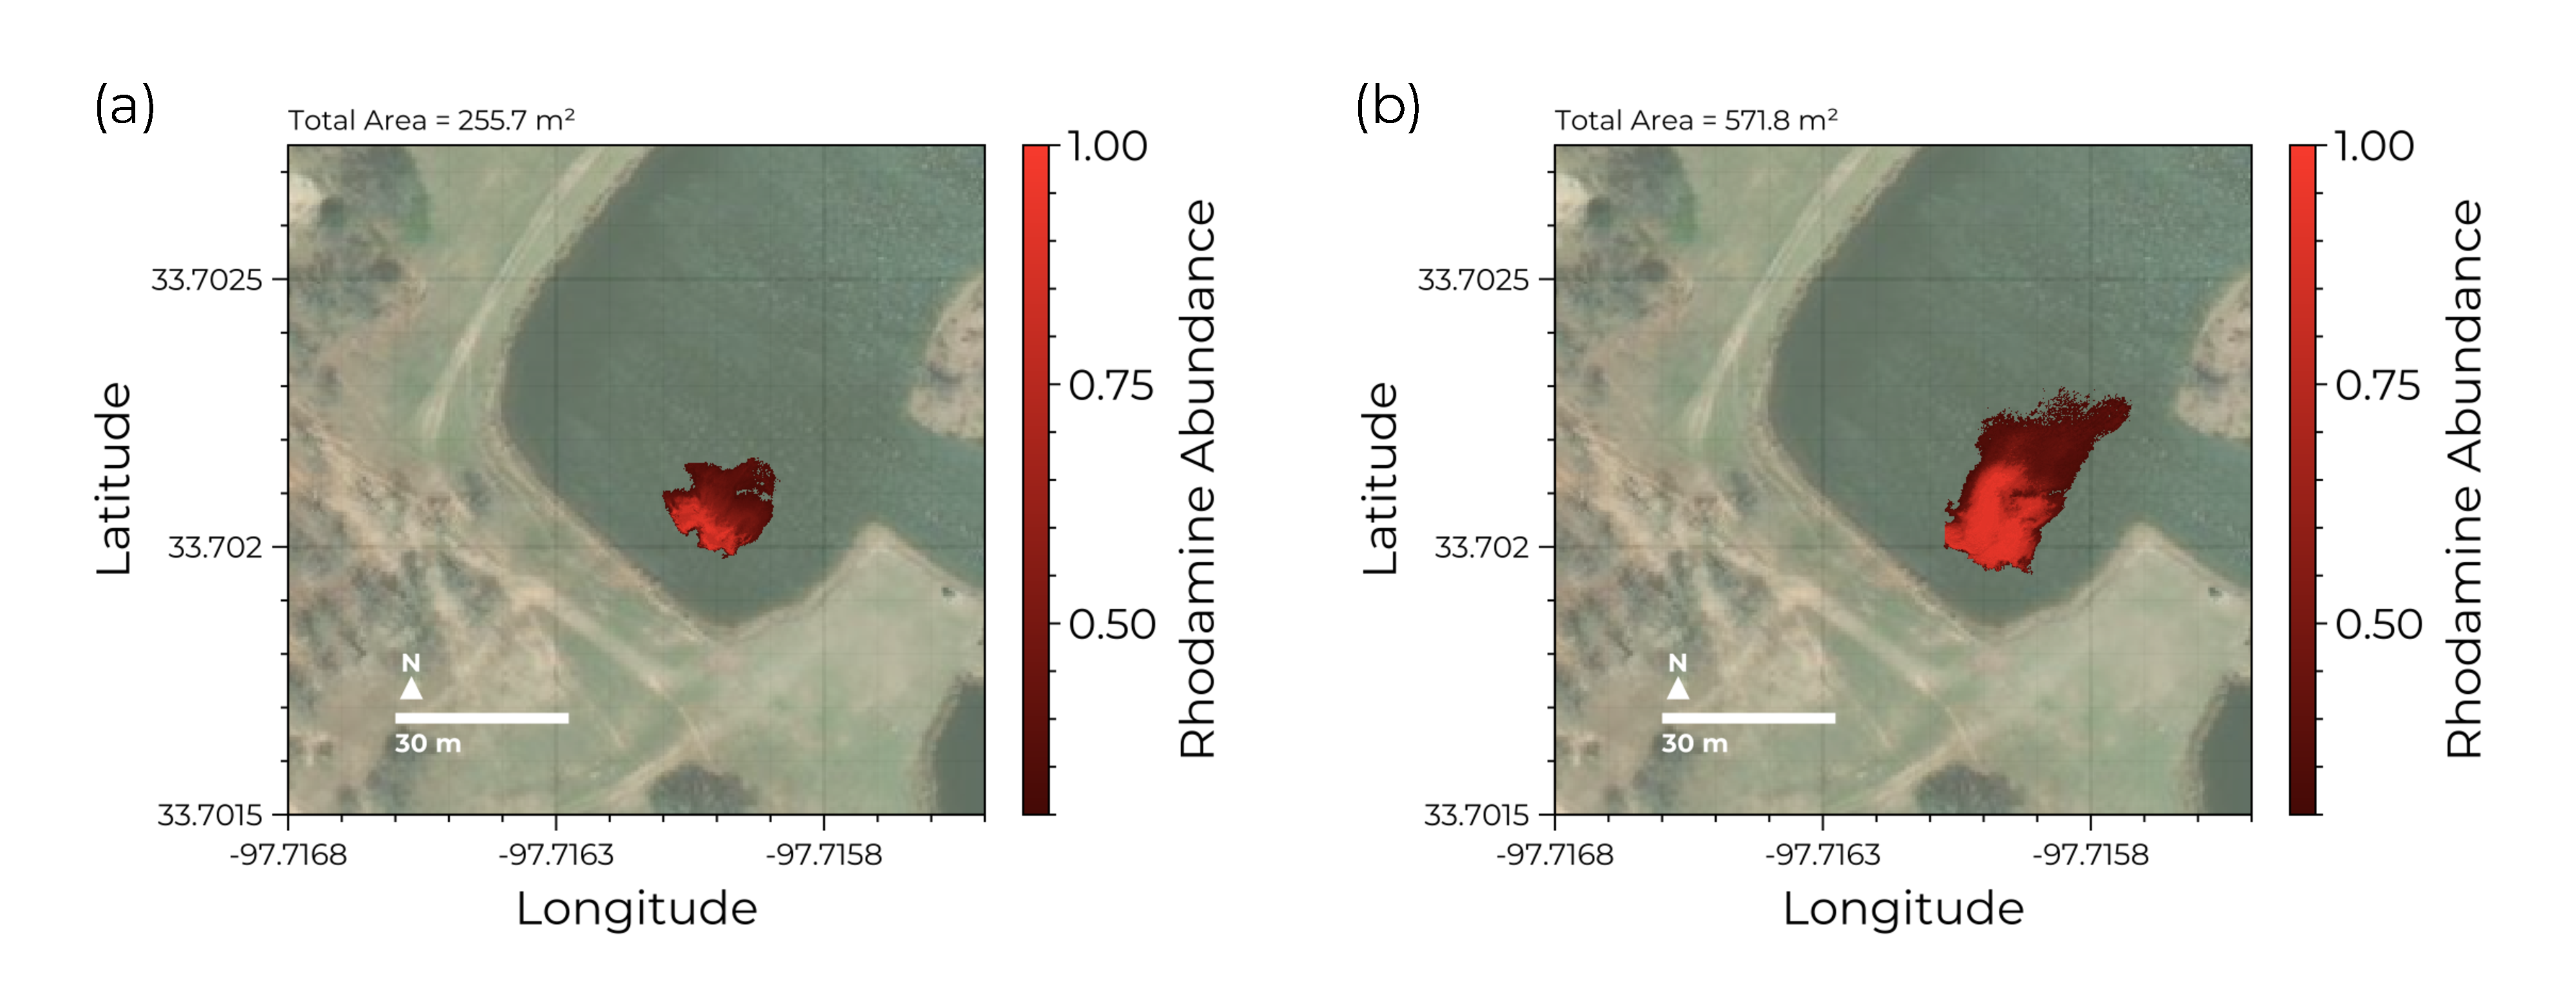
\includegraphics[width=\columnwidth]{robot-team-gsm/results/robot-team/plume-evo.pdf}
  \caption{Rhodamine plume evolution: Using the trained GSM we can track the
    dispersion of the rhodamine dye plume between successive drone flights.
    \textbf{(a)} The initial plume distribution after release. Here the dye
    subsumes an area of $255.7$ $\text{m}^2$. \textbf{(b)} The same plume imaged
    15 minutes later now extends across an area of $571.8$ $\text{m}^2$}
  \label{fig:plume-evo}
\end{sidewaysfigure}



% \begin{figure}[H]
%   \centering
%   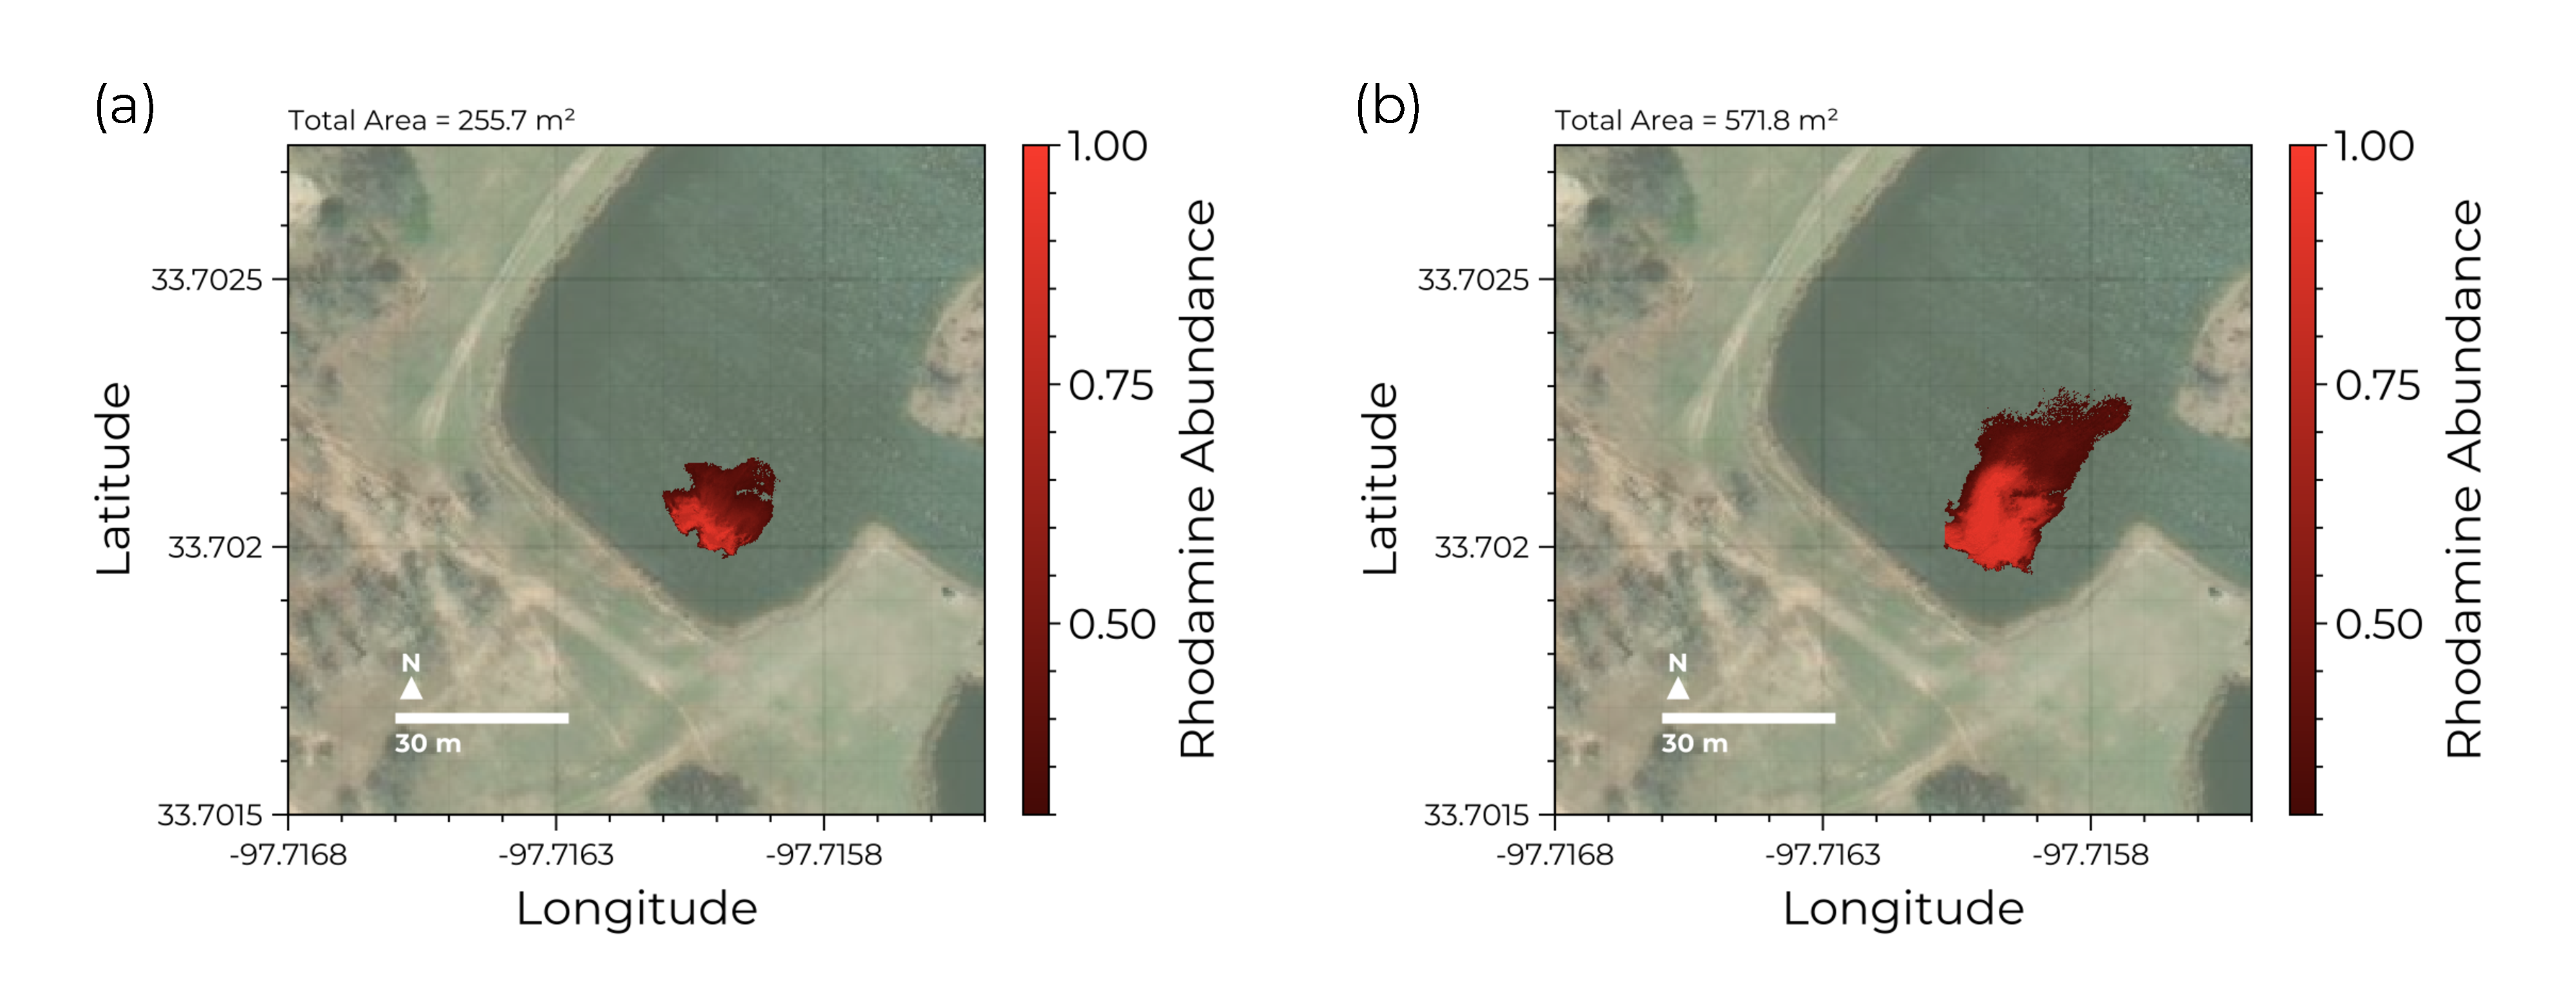
\includegraphics[width=\columnwidth]{robot-team-gsm/results/robot-team/plume-evo.pdf}
%   \caption{Rhodamine plume evolution: Using the trained GSM we can track the
%     dispersion of the rhodamine dye plume between successive drone flights.
%     \textbf{(a)} The initial plume distribution after release. Here the dye
%     subsumes an area of $255.7$ $\text{m}^2$. \textbf{(b)} The same plume imaged
%     15 minutes later now extends across an area of $571.8$ $\text{m}^2$}
%   \label{fig:plume-evo}
% \end{figure}


\clearpage
\newpage

\section{Discussion}



The proliferation of hyperspectral imaging technologies in the remote sensing and environmental monitoring communities underscores the need for efficient algorithms that can make sense of high-dimensional HSI. Of particular interest are unsupervised algorithms which utilize all available wavelength bins to identify unique source profiles that present realistic scenes. The GSM introduced in this paper is a novel method that simultaneously performs endmember extraction and spectral unmixing. Unlike popular endmember extraction algorithms, such as VCA, PPI, and N-FINDR, GSM does not assume the presence of pure pixels in HSI. Furthermore, the flexible structure of the mapping from the GSM latent space to the spectral data space allows the GSM to model non-linear mixing effects, distinguishing it from other widely used linear models such as NMF. Being a probabilistic model also enables the GSM to quantify the spectral variability through the precision parameter $\beta$ as indicated in Figure~\ref{fig:usgs-endmembers}. This additional capability is critical for analysis of realistic HSI where sensor noise, viewing geometry, and scene illumination all introduce uncertainty into extracted endmembers.

The growing popularity of deep learning methods has led many to explore applications of deep learning to the spectral unmixing problem. Variations in auto-encoder architectures are a popular choice for both endmember extraction and unmixing. For example, Borsoi et al. used a variational autoencoder to more accurately identify the spectral variability in a LMM \cite{borsoi2019deep}. Similarly, Palson et al. introduced an autoencoder with convolution layers to extend the LMM by incorporating spatial context from neighboring HSI pixels \cite{palsson2020convolutional}. However, the increased complexity of deep neural network approaches makes interpreting the latent space learned by encoder layers challenging and can dramatically increase training time and data volume requirements. In contrast, the latent space of the GSM is immediately interpretable due to the imposed simplex geometry, while the form of $\psi$ leaves room to explore a variety of non-linear mixing models. In this paper, $\psi$ was constructed to add non-linear effects as additions or perturbations to an underlying linear mixing model with the $\lambda_w$ hyperparameter provided to control the degree of non-linearity considered. In the original GTM formulation that inspired the GSM, the mapping $\psi$ strictly uses non-linear features generated by Gaussian RBFs. Alternatively, one could easily construct $\psi$ for specific non-linear models such as bilinear mixing by introducing features which depend on higher-order combinations of the latent space (abundance) coordinates. However, it is important to note that the EM algorithm formulated for GSM training is made possible due to the linear combination of activations $\phi(z)$ with model weights $\mathbf{W}$. For mixing models which instead depend non-linearly on weights $\mathbf{W}$, an EM algorithm may require iterative non-linear solves during each M step.

The main limitation of the GSM is the curse of dimensionality encountered when generating a grid on the $(N_v-1)$-simplex for large numbers of endmembers, $N_v$. This can be mitigated by instead randomly sampling points within the interior of the simplex using a uniform Dirichlet distribution to obtain a pre-determined number of nodes across the latent space. As the mixing coefficients $\pi_k$ are adapted during training, the variability in the spacing of the internodes should not significantly affect the performance of the model. In fact, this was confirmed for the simulated data set as summarized in Figure~\ref{fig:usgs-fits}. For considerably large data sets, the size of the responsibility matrix $\mathbf{R}$ can also lead to extended training times. This can be addressed by augmenting the EM procedure to updated using mini-batches of training samples during each E-step as described by Bishop et al. for the GTM in ref. \cite{gtm-developments}. Rather than updating the full responsibility matrix, a subset of $\mathbf{R}$ corresponding to a single batch of training data can be evaluated with all other entries kept constant. The GSM may also be extended in other ways, for example, by replacing the precision parameter $\beta$ with a covariance matrix to model wavelength-dependent spectral variability common to many hyperspectral imaging platforms. 

Based on the results of applying the GSM to real HSI as illustrated in Figure~\ref{fig:endmember-abundance-dist} and Figure~\ref{fig:plume-evo}, one clear application of the GSM is to contaminant identification and water quality assessment. Modern UAV platforms make it possible to rapidly image bodies of water where direct access for in-situ data collection is restricted. By equipping UAVs with hyperspectral imagers, the GSM can be used to identify abnormal spectral signatures corresponding to localized contaminant sources. Generating semantic segmentations of collected HSI as in panel b of Figure~\ref{fig:robot-team-endmembers} makes it easy to compare multiple HSI without resorting to pseudocolor images generated from a limited number of wavelength bands. Since the GSM models the distribution of all HSI spectra rather than individual parameters, it may also aid in-situ data collection by suggesting sampling points which maximize the area traversed in the GSM latent space rather than uniformly sampling across a wide spatial extent. Similar approaches have been developed to guide autonomous data collection vehicles by casting route planning as a prize collecting travelling salesman problem subject to resource constraints \cite{balas2007prize, suryan2020learning}.

As a final consideration, we note that the problem of endmember extraction and spectral unmixing for HSI is identical to source apportionment in the context of air quality. Here, the goal is to identify measurement profiles associated with sources of ambient air pollution based on measurements at a receptor site. A popular model for source apportionment studies is Positive Matrix Factorization (PMF) introduced by Paatero and Tapper \cite{pmf-orig, ulbrich2009interpretation}. Just like NMF, PMF decomposes measurements into a linear combination of source profiles and relative abundances subject to non-negativity constraints. These linear receptor models assume that the sources are not transformed during transport to the receptor, ignoring changes due to chemical reactions. Non-linear mixing models such as the GSM introduced here may, therefore, prove beneficial in this additional domain.






\chapter{Modeling Local Particulate Matter Dynamics with Time Delay Embeddings}\label{ch:havok}
% \chapter{Time-delay Embedding Models for Particulate Matter - Outlier Detection and Forecasting}\label{ch:havok}

\textcolor{magenta}{Should we keep the variogram stuff?}


The low-cost sensor network detailed in Chapter~\ref{ch:air-network} collects a
continuous stream of air quality data for a plethora of locations with high
temporal resolution ranging between $0.1$ to $1.0$ Hz. The real-time
visualization dashboards developed for the network offer immediate insight into
local air conditions. However, the challenge remains to extract actionable
insights from the large amounts of historical data. For example, we are concerned
with answering simple questions such as: \textit{What is the typical pattern of
  PM variability at this location}, \textit{Are changes in PM gradual or due to
  identifiable events?}, and \textit{Can we use historical PM measurements to
  provide insight into future air quality trends?}.

In this chapter, we propose a physics-based model rooted in Koopman operator
theory to address these questions by accurately capturing local PM dynamics.
Specifically, we extend the \textit{Hankel Alternative View of Koopman} (HAVOK)
framework introduced by Brunton et al. to apply to time series measurements of
PM data. In this data-driven approach PM dynamics are described via a simple
linear system with aperiodic external forcing. The forcing function extracted
from the model provides a clear method to identify abrupt pollution events from
historical data. The model can be used to provide accurate short-term forecasts.
Importantly, HAVOK models require few parameters, can be fit efficiently using
established numerical linear algebra routines, and are small enough to be
readily deployed directly onto sensor hardware.


\section{Motivation}


% Particulate matter (PM) dynamics exhibit complex behavior influenced by a variety of factors, including meteorological conditions, human activities, and atmospheric processes. PM concentrations typically follow well-established diurnal patterns, with peaks often occurring during morning and evening rush hours due to increased vehicular emissions, and lower concentrations observed during the midday when atmospheric dispersion is more effective (Zhang et al., 2012). Seasonal variations are also common, with higher PM levels in winter due to factors like heating emissions and temperature inversions that trap pollutants close to the ground (Cheng et al., 2013). Numerous models have been developed to analyze and forecast PM levels. These range from statistical models, such as autoregressive integrated moving average (ARIMA) models (Box et al., 1994), to more sophisticated machine learning approaches like neural networks, which can capture nonlinear relationships in the data (Zhang et al., 2020). Physics-based models, including chemical transport models (CTMs), provide detailed representations of atmospheric processes but require substantial computational resources and detailed input data (Seinfeld & Pandis, 2016). More recently, hybrid approaches combining machine learning with physical models have shown promise in improving forecast accuracy by leveraging the strengths of both methodologies (Bi et al., 2021). 

% ---

% **References:**

% 1. Zhang, Y., et al. (2012). "Diurnal variation in PM2.5 concentration and its causes." *Atmospheric Environment*, 45(8), 2017-2024.
% 2. Cheng, Y., et al. (2013). "Wintertime PM2.5 variations in China." *Environmental Pollution*, 182, 44-51.
% 3. Box, G.E.P., et al. (1994). *Time Series Analysis: Forecasting and Control*. Prentice Hall.
% 4. Zhang, Z., et al. (2020). "Air quality prediction using machine learning methods." *Journal of Environmental Management*, 242, 465-473.
% 5. Seinfeld, J.H., and Pandis, S.N. (2016). *Atmospheric Chemistry and Physics: From Air Pollution to Climate Change*. John Wiley & Sons.
% 6. Bi, J., et al. (2021). "A hybrid approach for PM2.5 forecasting: Combining physics-based models with deep learning." *Environmental Modelling & Software*, 139, 105014.



- Dynamics of particulate matter


- Time series models for PM (how good are forecasts)


- Value of a physics-based models, e.g. chemical transport

- Limitations of these models are due to poorly resolved meteorological
obsevations, for example, high resolution ECMWF analysis are at 0.1 x 0.1 km
grids with the lowest vertical model layer hundreds of meters above the ground.

- Many of these are being developed but have yet to see application to
realistic, noisy datasets




It should be noted that
despite the rapid pace of development in the fields of data-driven and
scientific machine learning, many recently developed techniques like the
Universal Differential Equations (UDEs), Hamiltonian Neural Networks, and others
have yet to see wide spread application on noisy, real-world datasets. Our
secondary goal for this chapter is therefore to demonstrate how, with some
slight modifications, these techniques can be applied to real-world problems.


In order to provide actionable insights we must be able to effectively model the
dynamics of our collected time series. In a perfect world, we would measure all
relevant physical quantities such that the time evolution of local air quality
at each sensor could be obtained by simulating the relevant micro-physics.
However, low cost sensor networks are not equipped with all the necessary
reference grade instruments needed to perform such simulations; accurate winds
speed and direction sensors alone can cost hundreds to thousands of dollars and
remote sensing data products are often unreliable at the ground level (i.e. in
the human head space). We therefore are motivated to develop techniques to model
our collected time series using only the data provided at a single node. There
are many approaches to this task in the statistics and machine learning
literature including statistical models like ARIMA and deep learning methods
like Recurrent Neural Networks \cite{intro-to-time-series-models,
  time-series-rnns}. While these methods can often lead to robust short term
predictions, they do not incorporate prior physics knowledge and therefore are
not primed to take advantage of underlying dynamical laws. Recently two
interesting physics-informed, data driven techniques have been developed for
just this type of scenario. The first we shall examine is the so-called
\textit{Hankel Alternative View Of Koopman} (HAVOK) framework which extends the
principle of dynamic mode decomposition to nonlinear systems
\cite{brunton-havok}. The second is an technique dubbed the \textit{Hamiltonian
  Neural Network} which extends the notion of a Neural Ordinary Differential
Equation to allow a neural network to learn coordinate transformations or the
original time series data which satisfy \textit{Hamiltons equations}
\cite{greydanus-hnn}.




Note the additional constraint that our model should be both physically
interpretable and small enough to be easily trained and deployed at scale. While
complicated DNN based approaches such as deep recurrent networks may provide an
ability to forecast, the size and training times involved for these approaches
are prohibitively high if we wish to train and deploy these models directly to
sensors in the network in an automated fashion. Also note the other HAVOK paper
which attempts to use HAVOK for predictions which showed that the HAVOK model
provides a superior one step prediction compared to other state of the art
models.


\section{Hankel Alternative View of Koopman}

\subsection{Koopman Operator Theory}

\subsection{Time-Delay Embeddings and Taken's Theorem}

\subsection{Hankel Alternative View of Koopman}


\subsection{Simple Example: Lorenz System}


\begin{figure}[h]
  \centering
  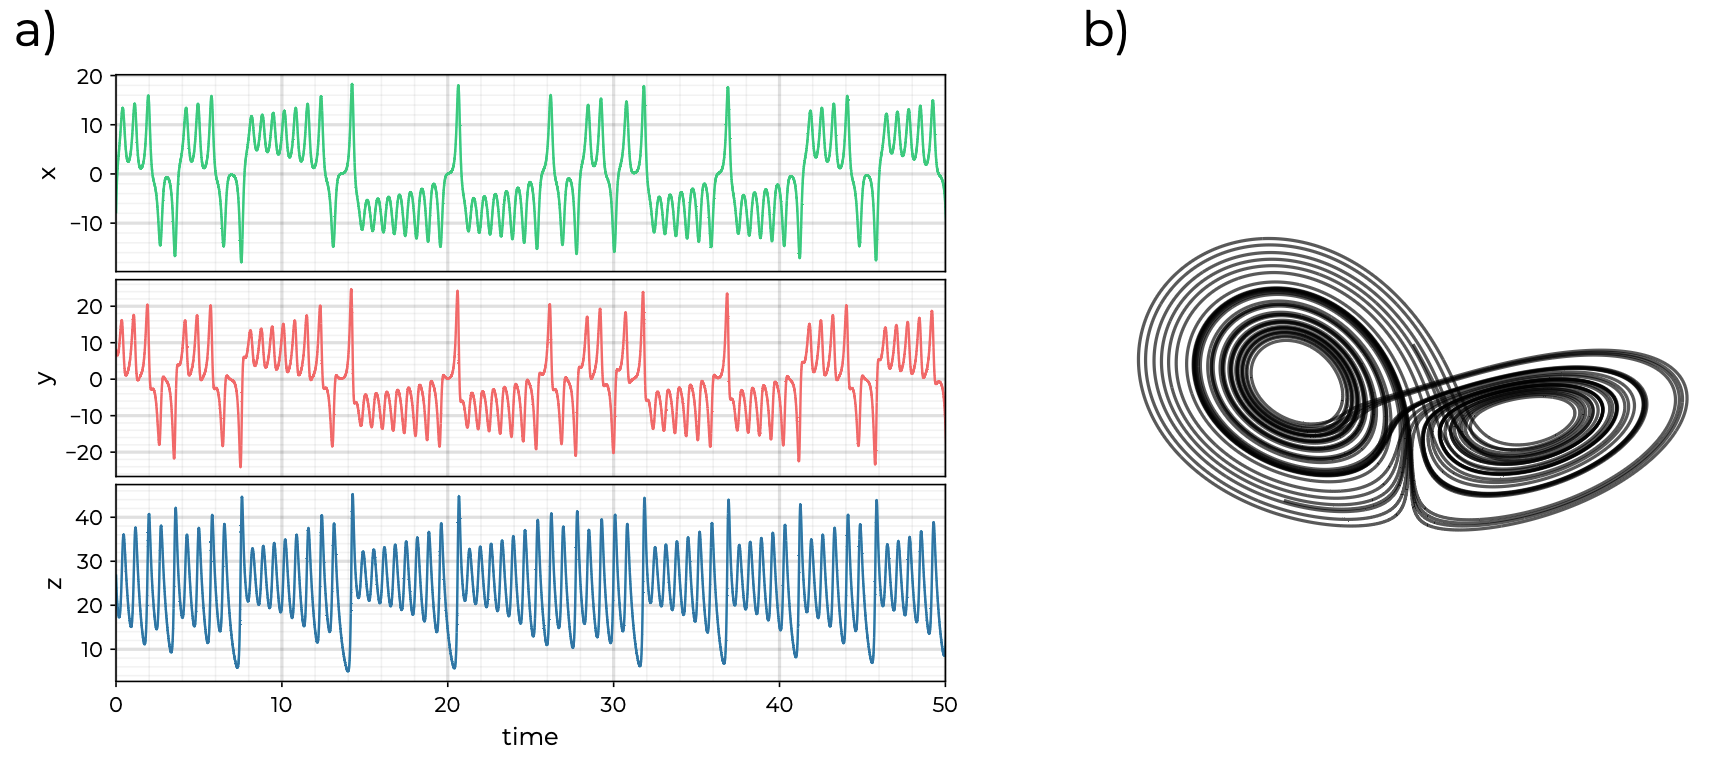
\includegraphics[width=\columnwidth]{havok/0-havok-lorenz/2__lorenz-orig.png}
  \caption{(\textbf{a}) Time series for the $x$, $y$, and $z$ components of the
    Lorenz system. (\textbf{b}) 3-dimensional visualization of the attractor
    formed from $x$, $y$, and $z$ components. We note that there are two clear
    lobes corresponding to the two attractors of the system.}
  \label{fig:lorenz-time-series-orig}
\end{figure}


\begin{figure}[h]
  \centering
  \includegraphics[width=0.5\columnwidth]{havok/0-havok-lorenz/1b_A-B-sHAVOK.pdf}
  \caption{Fitted operators $\mathbf{A}$ and $\mathbf{B}$ for the Lorenz system
    learned by the HAVOK model corresponding to the linear dynamics and
    intermittent forcing.}
  \label{fig:lorenz-A-B-heatmap}
\end{figure}


\begin{figure}[h]
  \centering
  \includegraphics[width=\columnwidth]{havok/0-havok-lorenz/3__havok-embedding.pdf}
  \caption{(\textbf{a}) Time series for first 3 components $v\_i$ of the HAVOK
    model. Original time series for each component are shown in blue. Time
    series predicted by the HAVOK model are overlaid in red. (\textbf(b)) The
    attractor formed by the first 3 embedding coordinates. By Taken's theorem,
    this attractor is diffeomorphic to the original attractor.}
  \label{fig:lorenz-havok-embedding}
\end{figure}



\begin{figure}[h]
  \centering
  \includegraphics[width=0.75\columnwidth]{havok/0-havok-lorenz/6__forcing-statistics.pdf}
  \caption{Proabability density function for forcing time series learned by the
    HAVOK model. The PDF is compared to a Gaussian fit for the same data. The
    wide tails of the PDF reflect that the forcing is intermittent.}
  \label{fig:lorenz-forcing-stats}
\end{figure}


\begin{figure}[h]
  \centering
  \includegraphics[width=\columnwidth]{havok/0-havok-lorenz/7__attractor-w-forcing.pdf}
  \caption{(\textbf{a}) The original time series $x(t)$ plotted with the squared
  forcing time series $v_r(t)$. Red colors indicate forcing above a chosen
  threshold which accurately identify lobe-switching events. (\textbf{b}) The
  Lorenz attractor colored using the same scheme.}
  \label{fig:lorenz-attractor-forcing}
\end{figure}



\begin{figure}[h]
  \centering
  \includegraphics[width=0.9\columnwidth]{havok/0-havok-lorenz/9__timeseries-reconstruction.pdf}
  \caption{The reconstructed time series for $x(t)$ using the learned HAVOK model.}
  \label{fig:lorenz-reconstruction}
\end{figure}




\section{Study Overview}

- Describe dataset, e.g. the specific central node, focus on PM 2.5, and the
collection period (find continuous data during no-rain period during the summer
of 2023 to evaluate HAVOK model independent of problems introduced by
hygroscopic growth)


\begin{figure}[h]
  \centering
  \includegraphics[width=0.8\columnwidth]{havok/1-havok-pm/1__timeseries-full-short.pdf}
  \caption{Time series of PM $2.5$ measurements from Central Hub 4 located in
    Planeo, Tx starting on 2023-08-04. This time series was selected during the
    long period of no precipitation during 2023 in order to limit the impact of
    hygroscopic growth on observed values. Note the occasional, thin vertical
    spikes corresponding to acute pollution events.}
  \label{fig:pm-timeseries-orig}
\end{figure}


\begin{figure}[h]
  \centering
  \includegraphics[width=0.7\columnwidth]{havok/1-havok-pm/1__pca-explained-variance.pdf}
  \caption{Explained variance of components from a principal component
    decomposition of the PM 2.5 time series sorted in decreasing order. A red
    line is superimposed indicating a $1\%$ explained variance. All components
    past the sixth contribute less than $1\%$ to the total explained variance. }
  \label{fig:pm-timeseries-pca}
\end{figure}


\section{Results}


\begin{figure}[h]
  \centering
  \includegraphics[width=0.8\columnwidth]{havok/1-havok-pm/1b__train-test-timeseries-short.pdf}
  \caption{Train-test split used for training the HAVOK model. To prevent data
    leaks, i.e. information from the future being incorporated into forecasts,
    the data was partitioned into two continuous sets to be used separately for
    model fitting and evaluation.}
  \label{fig:pm-train-test-split}
\end{figure}



\begin{table}[h]
  \caption{Results of HAVOK model hyperparameter search. Models were trained
    varying the embedding size ($N$), number of state variables $(r)$, and
    number of forcing terms ($n$). The top 10 models are presented here as
    evaluated by their RMSE and MAE values ranked in descending order.
    Additionally the top 3 models with $n=1$ are included for comparison.}
  \label{tab:havok-fit-results}
  \centering
  \begin{tabular}{ccccc} \hline
    \textbf{N} & \textbf{r} & \textbf{n} & \textbf{RMSE}  & \textbf{MAE} \\ \hline
    $30$ & $6$ & $5$ & $0.216703$ & $0.155912$ \\
    $45$ & $10$ & $5$ & $0.3649$ & $0.268842$ \\
    $30$ & $6$ & $4$ & $0.472797$ & $0.397746$ \\
    $45$ & $8$ & $5$ & $0.487448$ & $0.358938$ \\
    $30$ & $7$ & $5$ & $0.583654$ & $0.518485$ \\
    $30$ & $8$ & $5$ & $0.58551$ & $0.428986$ \\
    $30$ & $7$ & $4$ & $0.586575$ & $0.520145$ \\
    $30$ & $8$ & $4$ & $0.610296$ & $0.447673$ \\
    $30$ & $8$ & $3$ & $0.620928$ & $0.455369$ \\
    $60$ & $12$ & $5$ & $0.697797$ & $0.507499$ \\
    $\vdots$ & $\vdots$ & $\vdots$ & $\vdots$ & $\vdots$ \\
    $105$ & $3$ & $1$ & $1.48989$ & $1.09792$  \\
    $120$ & $3$ & $1$ &  $1.58473$ & $1.1494$ \\
    $180$ & $5$ & $1$ & $1.77659$ & $1.29506$ 
  \end{tabular}
\end{table}



\begin{figure}[h]
  \centering
  \includegraphics[width=0.75\columnwidth]{havok/2-havok-eval/1__predicted-ts-training.pdf}
  \caption{Time series predicted by HAVOK model with forcing functions provided.
  Inset into the figure is a subset of the }
  \label{fig:pm-havok-predictions}
\end{figure}




\begin{figure}[h]
  \centering
  \includegraphics[width=0.65\columnwidth]{havok/2-havok-eval/2__A-B-Havok.pdf}
  \caption{Operators learned by the HAVOK model with $r=6$ and $n=5$. We note
    that the $\mathbf{A}$ matrix displays the expected banded diagonal
    structure. Additionally, the values of the forcing matrix $\mathbf{B}$
    decrease with each column}
  \label{fig:pm-havok-operators}
\end{figure}



\begin{figure}[h]
  \centering
  \includegraphics[width=0.35\columnwidth]{havok/2-havok-eval/3__A-eigvals.pdf}
  \caption{Eigenvalues of the learned HAVOK operator $\mathbf{A}$ visualized in
    the complex plane. We note that no eigenvalues had any postive real
    component reflecting the model's stability for integration over long time periods. }
  \label{fig:pm-havok-eigvals}
\end{figure}



\begin{figure}[h]
  \centering
  \includegraphics[width=0.65\columnwidth]{havok/2-havok-eval/4__forcing-statistics.pdf}
  \caption{Probability density function evaluated for the first forcing function
  compared to a zero-mean Gaussian distribution fit to the forcing data. The
  wide tails of the estimated distribution reflect the intermittent activation
  of forcing.}
  \label{fig:pm-forcing-stats}
\end{figure}


\begin{figure}[h]
  \centering
  \includegraphics[width=\columnwidth]{havok/2-havok-eval/forcing-time-series.pdf}
  \caption{(\textbf{a}) Time series of first forcing function activation for the
    duration of the training set. (\textbf{b}) The same time series zoomed in to
    the first hours. The mean value for the forcing function was $7.94\times
    10^5$ reflecting the fact that the learned forcing functions tend to be
    centered about zero with no long-term trend.}
  \label{fig:pm-forcing-time-series}
\end{figure}


\begin{figure}[h]
  \centering
  \includegraphics[width=\columnwidth]{havok/2-havok-eval/6__timeseries-with-forcing.pdf}
  \caption{The original PM 2.5 time series plotted together with the squared
    value of the first forcing function, $\lVert  f_1(t) \rVert^2$. By
    thresholding the values of $f_1$, the intermittent PM spikes are easily
    identified. }
  \label{fig:pm-time-series-w-forcing}
\end{figure}




\begin{table}[h]
  \caption{Evaluation of HAVOK forecasting performance as a function of
    prediction horizon from 10 seconds to 4 minutes.}
  \label{tab:havok-forecasting-results}
  \centering
  \begin{tabular}{ccccccc} \hline
    \textbf{Duration} & \textbf{RMSE}  & \textbf{RMSE} & \textbf{MAE}   & \textbf{MAE}  & \textbf{MAPE}  & \textbf{MAPE} \\
                      & \textbf{train} & \textbf{test} & \textbf{train} & \textbf{test} & \textbf{train} & \textbf{test} \\\hline
    10 sec.	  & 0.0611 & 0.0589 & 0.0415 & 0.0415 & 0.0054 & 0.0057 \\
    1 min.	  & 0.2555 & 0.2398 & 0.1757 & 0.1720 & 0.0231 & 0.0235 \\
    2 min.	  & 0.7056 & 0.6764 & 0.4874 & 0.4945 & 0.0640 & 0.0674 \\
    3 min.	  & 1.0552 & 1.0366 & 0.7290 & 0.7691 & 0.0957 & 0.1052 \\
    4 min.	  & 1.3759 & 1.3567 & 0.9530 & 1.0185 & 0.1252 & 0.1389 \\
    5 min. 	  & 1.6696 & 1.6530 & 1.1611 & 1.2475 & 0.1525 & 0.1703
  \end{tabular}
\end{table}






\begin{figure}[h]
  \centering
  \includegraphics[width=\columnwidth]{havok/3-forcing-fit/forecast-scatter.pdf}
  \caption{Scatter diagrams for multistep forecasts. (\textbf{a}) 10 second
    forecast. (\textbf(b)) 1 minute forecast. (\textbf{c}) 2 minute forecast.
    (\textbf{d}) 5 minute forecast. The integration time step was $\Delta t =
    10$ s so that a 5 minute forecast corresponds to a 30 step future prediction.}
  \label{fig:pm-time-series-w-forcing}
\end{figure}



% \chapter{A Chemical Data Assimilation Framework for Indoor Air Quality Assessment}\label{ch:autochem}


\section{Gaussian Processes}

\section{Adjoint Methods for Optimization}
\subsection{Linear Systems}
\subsection{Nonlinear Systems}
\subsection{Ordinary Differential Equations}


\section{Data Assimilation}
\subsection{Kalman Filter}
\subsection{Extended Kalman Filter}
\subsection{Continuous-discrete Extended Kalman Filter}
\subsection{3d-Var}
\subsection{4d-Var}

\section{Physics of Chemical Reactions: Chemical Reaction Kinetics}
\subsection{Overview}
\subsection{Chemical Equilibrium and the Law of Mass Action}
\subsection{Reaction Rate Laws}

\section{Summary of Chemical Mechanism Kinetics}

\section{Characterization of Photolysis Rates}
\subsection{Absorption Cross Sectionss}
\subsection{Quantum Yields}
\subsection{Photolysis Rate Determination}

\section{Chemical Data Assimilation}

\section{Results}

\section{Discussion}


\chapter{Future Work}\label{ch:future-work}

\section{Robot Team}

Minaturization of drones - next generation hyperspectral imagers (smaller) on smaller drones with additional payloads for visible and thermal imagers (not previously utilized)

Multi-sensor fusion and super resolution, e.g. use fine spatial resultion of visible imager together with spectral resolution of HSI and thermal to create a blended data product

Combine drone based imaging with remote sensing hyperspectral data, e.g. Enmap, PACE, etc...

Drone swarms for faster data collection

Additional data collection (can we test the generalizability across water bodies)

Additional ions with application to battery stuff...

\section{GTM}

GTM for guided data collection viat prize-collecting travelling salesman problem.

GTM for dust source identification. We can encourage finer cluserting behavior by augmenting the GTM to use adaptive mixing coefficients $\pi_k$ as we did for the GSM.

Batch version implementation of the GTM for \textit{big} datasets and online learning.

\section{GSM}

GSM for algal bloom identifiaction using remotely sensed hyperspectral imagery.

GSM for source apportionment of air quality measurements

Batch version of the GSM for \textit{big} dtaasets.


\section{PM Modeling}

Using HAVOK model to automatically identify pollution events and generate short term predictions near real time.

\section{Air Parcel Back Trajectories}

Compute back trajectories of PM data using meteorological analysis (and re-analyses).

Applications to human health outcomes: Alzheimers


\section{Chemical Data Assimilation}

Air quality chamber.







\chapter{Conclusions}\label{ch:conclusions}

\textcolor{red}{\textbf{Robot Team Supervised:}}
In this study, we address two key limitations of current remote sensing
approaches to characterize water quality: namely, the limited spatial, spectral,
and temporal resolution provided by existing satellite platforms and the lack of
comprehensive in situ measurements needed to validate remote sensing data
products. By equipping an autonomous USV with a suite of reference sensors, we
rapidly collect significantly more data than existing approaches that rely on
the collection of individual samples for lab analysis or are constrained to
continuous sensing at fixed sites. Utilizing an autonomous UAV equipped with a
hyperspectral imager in tandem with the USV allows us to quickly generate
aligned datasets that are used to train machine learning models mapping measured
reflectance spectra to the desired water quality variables. By virtue of this
increased data volume, we are able to simultaneously estimate the uncertainty of
our models by using conformal prediction. Finally, the hyperspectral data cube
processing workflow employed onboard the UAV makes it possible to deploy these
trained models to swiftly generate maps of the target variables across bodies of
water. The rapid turnaround time from data collection to model deployment is
critical for real-time water quality evaluation and risk assessment.




\textcolor{red}{\textbf{Robot Team GTM}}
In this study, we present  GTM as a useful unsupervised method for the visualization of UAV-based hyperspectral imagery and associated extraction of spectral endmembers. Using data collected at a North Texas pond, we demonstrate how the latent space of the GTM can be used to visualize the distribution of observed reflectance spectra revealing the small-scale spatial variability of water composition. Spectral signatures extracted from GTM nodes are used to successfully map the abundance of algae near the shore and to track the evolution of a rhodamine tracer dye plume. These examples illustrate the power of combining unsupervised learning with UAV-based hyperspectral imaging for the characterization of water composition. Future work will further develop the GTM as a tool to guide in situ data collection and enable contaminant localization for real-time applications.




\appendix % required only if you have appendixes
\chapter{Spectral Indices}\label{appendix:spectral-indices}

For hyperspectral reflectance indices, we make the
following identifications:

\begin{align}\label{eq:ref-bands}
\begin{split}
    \rho_b &= \rho(440 \text{ nm}) \\
    \rho_g &= \rho(550 \text{ nm}) \\
    \rho_b &= \rho(650 \text{ nm}) \\
    \rho_{nir} &= \rho(860 \text{ nm}).
\end{split}
\end{align}

We also define $\rho_{far} = \rho(1009 \text{ nm})$ as the band
representing the farthest infrared bin for our hyperspectral imager
which we use instead of the usual SWIR band.

\begin{sidewaystable}[p]
  \caption{Spectral indices supplied as extra features to each ML model. For each index, $\rho_{\lambda}$ denotes the reflectance at wavelength $\lambda$ used to compute the index. Reflectances $\rho_b$, $\rho_g$, etc are as defined in Equation \ref{eq:ref-bands}. Where relevent, $\gamma = 1$ and $\eta = 2(\rho_{nir}^2 - \rho_r^2) + 1.5\rho_{nir} + 0.5\rho_r$ have been used.}
  \label{table:spectral-indices}
  \begin{center}
  %\begin{tabular}{lcp{2.5in}}\hline
  \begin{tabular}{lcc}\hline
  \textbf{Spectral Index} & \textbf{Acronymn} & \textbf{Formula} \\ \hline
  Difference Vegetation Index & DVI & $\dfrac{2.5(\rho_{nir} - \rho_r)}{\rho_{nir} + 6\rho_r - 7.5\rho_b + 1}$ \\
  Global Environmental Monitoring Index & GEMI & $\eta(1 - 0.25\eta) - \dfrac{\rho_r - 1.125}{1 - \rho_r}$ \\
  Green Atmospherically Resistant Index & GARI & $\dfrac{\rho_{nir} - (\rho_g - \gamma(\rho_b - \rho_r))}{\rho_{nir} + (\rho_g - \gamma (\rho_b - \rho_r))}$ \\
  Green Chlorophyll Index & GCI & $\dfrac{\rho_{nir}}{\rho_g} - 1$ \\
  Green Difference Vegetation Index & GDVI & $\rho_{nir} - \rho_g$ \\
  Green Leaf Index & GLI & $\dfrac{(\rho_g - \rho_r) + (\rho_g - \rho_b)}{2 \rho_g + \rho_r + \rho_b}$ \\
  Green Normalized Difference Vegetation Index & GNDVI & $\dfrac{\rho_{nir} - \rho_g}{\rho_{nir} + \rho_g}$ \\
  Green Optimized Soil Adjusted Vegetation Index & GOSAVI & $\dfrac{\rho_{nir} - \rho_g}{\rho_{nir} + \rho_g + 0.16}$ \\
  Green Ratio Vegetation Index & GRVI & $\dfrac{\rho_{nir}}{\rho_g}$ \\
  Green Soil Adjusted Vegetation Index & GSAVI & $\dfrac{1.5(\rho_{nir} - \rho_g)}{\rho_{nir} + \rho_g + 0.5}$ \\
  Infrared Percentage Vegetation Index & IPVI & $\dfrac{\rho_{nir}}{\rho_{nir} + \rho_r}$ \\
  Leaf Area Index & LAI & $3.618 \left(\dfrac{2.5 (\rho_{nir} - \rho_r)}{\rho_{nir} + 6\rho_r - 7.5 \rho_b + 1}\right) - 0.118$ \\
  Modified Non-Linear Index & MNLI & $\dfrac{1.5(\rho_{nir}^2 - \rho_r)}{\rho_{nir}^2 + \rho_r + 0.5}$ \\
  Modified Soil Adjusted Vegetation Index 2 & MSAVI2 & $\dfrac{2\rho_{nir} + 1 - \sqrt{(2\rho_{nir} + 1)^2 - 8(\rho_{nir} - \rho_r)}}{2}$ \\
  Modified Simple Ratio & MSR & $\dfrac{\rho_{nir}/\rho_r - 1}{\sqrt{\rho_{nir} / \rho_r} + 1}$ 
  \end{tabular}
  \end{center}
\end{sidewaystable}


\begin{sidewaystable}[p]
  \contcaption
  \begin{center}
  \begin{tabular}{lcc}\hline
  \textbf{Spectral Index} & \textbf{Acronymn} & \textbf{Formula} \\ \hline
  Non-Linear Index & NLI & $\dfrac{\rho_{nir}^2 - \rho_r}{\rho_{nir}^2 + \rho_r}$ \\
  Normalized Difference Vegetation Index & NDVI & $\dfrac{\rho_{nir} - \rho_r}{\rho_{nir} + \rho_r}$ \\
  Normalized Pigment Chlorophyll Index & NPCI & $\dfrac{\rho_{680} - \rho_{430}}{\rho_{680} + \rho_{430}}$ \\
  Optimized Soil Adjusted Vegetation Index & OSAVI & $\dfrac{\rho_{nir} - \rho_r}{\rho_{nir} + \rho_r + 0.16}$ \\
  Renormalized Difference Vegetation Index & RDVI & $\dfrac{\rho_{nir} - \rho_r}{\sqrt{\rho_{nir} + \rho_r}}$ \\
  Soil Adjusted Vegetation Index & SAVI & $\dfrac{1.5(\rho_{nir} - \rho_r)}{\rho_{nir} + \rho_r + 0.5}$ \\
  Simple Ratio & SR & $\dfrac{\rho_{nir}}{\rho_r}$ \\
  Transformed Difference Vegetation Index & TDVI & $\dfrac{1.5\rho_{nir} - \rho_r}{\sqrt{\rho_{nir}^2 + \rho_r + 0.5}}$ \\
  Triangular Greenness Index & TGI & $\dfrac{(\lambda_r-\lambda_b)(\rho_r- \rho_g) - (\lambda_r-\lambda_g)(\rho_r - \rho_b)}{2}$ \\
  Visible Atmospherically Resistant Index & VARI & $\dfrac{\rho_g - \rho_r}{\rho_g + \rho_r - \rho_b}$ \\
  Wide Dynamic Range Vegetation Index & WDRVI & $\dfrac{0.2 \rho_{nir} - \rho_r}{0.2 * \rho_{nir} + \rho_r}$ \\
  Atmospherically Resistant Vegetation Index & ARVI & $\dfrac{\rho_{800} - (\rho_{800} - 1(\rho_{450} - \rho_{680}))}{\rho_{800} + (\rho_{680} - 1 (\rho_{450} - \rho_{680}))}$ \\
  Modified Chlorophyll Absorption Ratio Index & MCARI & $((\rho_{700} - \rho_{670}) - 2(\rho_{700} - \rho_{550}))\dfrac{\rho_{700}}{\rho_{670}}$ \\
  Modified Chlorophyll Absorption Ratio Index Improved & MCARI2 & $\dfrac{1.5( 2.5(\rho_{800} - \rho_{670}) - 1.3 (\rho_{800} - \rho_{550}))}{\sqrt{(2\rho_{800} + 1)^2 - (6\rho_{800} - 5 \sqrt{\rho_{670}}) - 0.5}}$ \\
  Modified Red Edge Normalized Difference Vegetation Index & MRENDVI & $\dfrac{\rho_{750} - \rho_{705}}{\rho_{750} + \rho_{705} - 2\rho_{445}}$ \\
  Modified Red Edge Simple Ratio & MRESR & $\dfrac{\rho_{750} - \rho_{445}}{\rho_{705} - \rho_{445}}$
  \end{tabular}
  \end{center}
\end{sidewaystable}

\begin{sidewaystable}[p]
  \contcaption
  \begin{center}
  \begin{tabular}{lcc}\hline
  \textbf{Spectral Index} & \textbf{Acronymn} & \textbf{Formula} \\ \hline
  Modified Triangular Vegetation Index & MTVI & $1.2 (1.2 (\rho_{800} - \rho_{550}) - 2.5 (\rho_{670} - \rho_{550}))$ \\
  Modified Triangular Vegetation Index & MTVI & $1.2 (1.2 (\rho_{800} - \rho_{550}) - 2.5 (\rho_{670} - \rho_{550}))$ \\
  Red Edge Normalized Difference Vegetation Index & RENDVI & $\dfrac{\rho_{750} - \rho_{705}}{\rho_{750} + \rho_{705}}$ \\
  Transformed Chlorophyll Absorption Reflectance Index & TCARI & $3\left((\rho_{700} - \rho_{670}) - 0.2(\rho_{700} - \rho_{550})\dfrac{\rho_{700}}{\rho_{670}}\right)$ \\
  Triangular Vegetation Index & TVI & $0.5(120 (\rho_{750} - \rho_{550}) - 200 (\rho_{670} - \rho_{550}))$\\
  Vogelmann Red Edge Index 1 & VREI1 & $\dfrac{\rho_{740}}{\rho_{720}}$ \\
  Vogelmann Red Edge Index 2 & VREI2 & $\dfrac{\rho_{734} - \rho_{747}}{\rho_{715} + \rho_{726}}$ \\
  Vogelmann Red Edge Index 3 & VREI3 & $\dfrac{\rho_{734} - \rho_{747}}{\rho_{715} + \rho_{720}}$ \\
  Photochemical Reflectance Index & PRI & $\dfrac{\rho_{531} - \rho_{570}}{\rho_{531} + \rho_{570}}$ \\
  Structure Insensitive Pigment Index & SIPI & $\dfrac{\rho_{800} - \rho_{445}}{\rho_{800} + \rho_{680}}$ \\
  Structure Independent Pigment Index & SIPI1 & $\dfrac{\rho_{445} - \rho_{800}}{\rho_{670} - \rho_{800}}$ \\
  Plant Senescence Reflectance Index & PSRI & $\dfrac{\rho_{680} - \rho_{500}}{\rho_{750}}$ \\
  Anthocyanin Reflectance Index 1 & ARI1 & $\dfrac{1}{\rho_{550}} - \dfrac{1}{\rho_{700}}$ \\
  Anthocyanin Reflectance Index 2 & ARI2 & $\left(\dfrac{1}{\rho_{550}} - \dfrac{1}{\rho_{700}}\right)\rho_{800}$ \\
  Carotenoid Reflectance Index 1 & CRI1 & $\dfrac{1}{\rho_{510}} - \dfrac{1}{\rho_{550}}$ \\
  Carotenoid Reflectance Index 2 & CRI2 & $\dfrac{1}{\rho_{510}} - \dfrac{1}{\rho_{700}}$ \\
  Normalized Difference Water Index 1 & NDWI1 & $\dfrac{\rho_g - \rho_{nir}}{\rho_g + \rho_{nir}}$ \\
  Normalized Difference Water Index 2 & NDWI2 & $\dfrac{\rho_{nir} - \rho_{far}}{\rho_{nir} + \rho_{far}}$
  \end{tabular}
  \end{center}
\end{sidewaystable}



\begin{sidewaystable}[p]
  \contcaption
  \begin{center}
  \begin{tabular}{lcc}\hline
  \textbf{Spectral Index} & \textbf{Acronymn} & \textbf{Formula} \\ \hline
  Modified Normalized Difference Water Index & MNDWI & $\dfrac{\rho_g - \rho_{far}}{\rho_g + \rho_{far}}$ \\
  Water Band Index & WBI & $\dfrac{970}{900}$ \\
  Anthocyanin Content Index & ACI & $\dfrac{\rho_g}{\rho_{nir}}$ \\
  Chlorophyll Index Red Edge & CIre & $\dfrac{\rho_{nir}}{\rho_{705}} - 1$ \\
  Modified Anthocyanin Reflectance Index & MARI & $\left(\dfrac{1}{\rho_{550}} - \dfrac{1}{\rho_{700}} \right)\rho_{nir}$ \\
  Moisture Stress Index & MSI & $\dfrac{\rho_{far}}{\rho_{nir}}$ \\
  MERIS Terrestrial Chlorophyll Index & MTCI & $\dfrac{\rho_{753.75} - \rho_{708.75}}{\rho_{708.75} - \rho_{681.25}}$ \\
  Normalzied Difference Infrared Index & NDII & $\dfrac{\rho_{nir} - \rho_{far}}{\rho_{nir} + \rho_{far}}$ \\
  Normalized Difference Red Edge & NDRE & $\dfrac{\rho_{790} - \rho_{720}}{\rho_{790} + \rho_{720}}$ \\
  Red Green Ratio Index & RGRI & $\dfrac{\rho_r}{\rho_g}$ \\
  Red Edge Vegetation Stress Index & RVSI & $\dfrac{\rho_{714} + \rho_{752}}{2} - \rho_{733}$
  \end{tabular}
  \end{center}
\end{sidewaystable}






\chapter{Derivatives of the complete data log-likelihood for the GSM}\label{appendix:gsm-deriv}


The penalized complete data log-likelihood function for the the GSM is given by
\begin{equation}
\begin{aligned}
    Q &= \sum_n^N\sum_k^K R_{kn} \left(\ln\pi_k + \frac{D}{2}\ln\left(\frac{\beta}{2\pi}\right) - \frac{\beta}{2}\sum_d^D\left(\sum_m^M W_{dm}\Phi_{km} - X_{nd}\right)^2\right) \\
    &\qquad + \frac{N_vD}{2}\ln\left(\frac{\lambda_e}{2\pi}\right) - \frac{\lambda}{2}\sum_d^D \sum_{m=1}^{N_v} W_{dm}^2  \\
    &\qquad + (M-N_v)D\ln\left(\dfrac{\lambda_w}{2}\right) - \lambda_w\sum_d^D\sum_{m=N_v+1}^{M} W_{dm}
\end{aligned}
\end{equation}
Differentiating with respect to $W_{st}$, we obtain
\begin{align*}
  \frac{\partial Q}{\partial W_{st}} &= \sum_n^N\sum_k^K R_{kn}(-\beta)\sum_d^D \left( \sum_m^M W_{dm}\Phi_{km} - X_{nd}\right)\frac{\partial}{\partial W_{st}}\left( \sum_\lambda W_{d\lambda}\Phi_{k\lambda} \right) - \Lambda_{st} \\
                                     &= \sum_n^N\sum_k^K (-\beta)R_{kn}\sum_d\left( \sum_m W_{dm}\Phi_{km} - X_{nd} \right)\Phi_{k\lambda}\delta_{ds}\delta_{\lambda t} - \Lambda_{st} \\
                                     &= \sum_n^N\sum_k^K (-\beta)R_{kn}\left( \sum_m W_{sm}\Phi_{km}\Phi_{kt} - X_{ns}\Phi_{kt}\right) - \Lambda_{st} \\
  &= \sum_n^N\sum_k^K \beta X_{ns}R_{kn}\Phi{kt} - \sum_k^K\sum_m^M\beta W_{sm}\Phi_{km}G_{kk}\Phi_{kt} - \Lambda_{st}
\end{align*}
where $\Lambda$ is a matrix with elements
\begin{equation}
  \Lambda_{st} = \begin{cases}
    \lambda_eW_{st}, & m\leq N_v \\
    \lambda_w, & m > N_v
  \end{cases}
\end{equation}
and $\mathbf{G}$ is a diagonal matrix with entries $G_{kk} = \sum_n R_{kn}$.
Translating from index notation, we obtain the final expression
\begin{equation}
    \frac{\partial Q}{\partial \mathbf{W}} = -\beta \mathbf{W}\mathbf{\Phi}^T\mathbf{G}\mathbf{\Phi} - \mathbf{\Lambda} + \beta \mathbf{X}^T\mathbf{R}^T\mathbf{\Phi}
\end{equation}


%%\chapter{Chemical Reaction Mechanisms}\label{appendix:mechanisms}

\textcolor{red}{UPDATE REQUIRED!}

%% \chapter{Reproducible Research Techniques}
\textcolor{red}{\textbf{UPDATE REQUIRED!}}

\section{Environment Management in Julia}
\section{Version Control (git)}
\section{CI/CD with github worfklows}
discuss automated tests as well as automatic document generation here

\section{Literate Programming and Automatic Documentation with Quarto}
\section{Containerization with Docker and Docker Compose}
Discuss NodeRed, InfluxDB, Grafana, etc...


%% \chapter{Optimization Methods}

Describe standard gradient descent and it's utility for machine learning. Expand to briefly describe the extensions used in our work:
\begin{itemize}
\item Gradient Descent
\item Gradient Descent with Momentum
\item ADAM
\item BFGS
\item LBFGS
\item The method we used for the variogram method that works specifically for quadratic loss functions...
\end{itemize}

We should also comment on which particular methods are best (and when)


%% \chapter{High Performance Computing}


Provide an overview of relevant concepts in high performance computing i.e.
\begin{itemize}
\item slurm
\item multi-threading
\item parallelization (distribured computing)
\item Memory management (i.e. preallocating data containers and writing functions that mutate, not allocate)
\end{itemize}


%% \chapter{A Chemical Data Assimilation Framework for Indoor Air Quality}




\section{Physics of Chemical Reactions: Chemical Reaction Kinetics}

\subsection{Overview}

Since the early successes of Newton's descriptions of mechanics by means of simple forces acting on masses, scientists have sought to understand the dynamics of chemical reactions in terms of the detailed microphysics of molecular collisions. As we shall see, this approach can be utilized productively to justify the complicated temperature and pressure dependence of the reaction rate coefficients of many elementary reaction. However, even when considering the asymmetric structure of many molecules, and therefore, the dependence on orientation at the collision site, kinetic theory alone is unable to model reaction rates in all relevant temperature and pressure regimes. To do this, one can utilize the modern treatment of \textit{Potential Energy Surface} (PES) theory together with the notion of short-lived, unstable intermediate reaction states to calculate reaction rate coefficient functions for specific reactants. \textit{Ab initio} solution of the Schrodinger equation for the relevant nuclear geometries ($3N$ reaction coordinates for $N$ atoms) together with scattering and spectroscopic methods as suggested by \cite{transition-state-spectroscopy-bimol} have led to significant improvements in our understanding of reaction dynamics.



\begin{figure}[h]
  \centering
  \includegraphics[width=0.85\textwidth]{introduction/reaction-timescales.png}
  \caption{An illustration of the broad range of reaction time scales from the long-lived nuclear decay to rapid degradation of molecules by photolysis. Figure taken from \cite{arnaut2006chemical}}
  \label{fig:reaction-timescales}
\end{figure}


However the computational complexity of this task makes it prohibitively expensive to perform at the scale required for our desired chemical mechanism which consists of many hundreds to thousands of reactants together with as many as 16,000 unique reactions. Therefore in the following discussion, we shall primarily utilize the kinetic theory to justify the functional form for \textit{most} rate coefficients with some reference to the extensions made by PES theory. We note that in practice, kinetic evaluations such as the periodic reports from the NASA Jet Propulsion Laboratory \cite{jpl-kinetic-evaluation-2020} utilize (justified) empirical fits to provide suggested functional forms for reaction rate coefficients.

\subsection{Chemical Equilibrium and the Law of Mass Action}

Before outlining the dynamics involved during complex chains of chemical reactions, it is worth spending some time to consider how we should treat chemical equilibrium. Usually in these scenarios we can not hold the internal energy fixed due to interactions with the environment, but rather, the temperature and pressure can often be treated as so. For example, we may be interested in gas-phase reactions occurring in ambient indoor air at or near standard temperature and pressure. In such scenarios, one finds the relevant potential energy to be the Gibbs, given by
\begin{equation}
  G = U - TS + PV,
\end{equation}
which is minimized in equilibrium under constant temperature and pressure.

This equation leads to the convenient thermodynamic identity
\begin{equation}
  dG = -SdT + VdP + \sum_i \mu_i dN_i
\end{equation}
from which we may identify the \textit{chemical potential} of the $i^{th}$ species as
\begin{equation}
  \mu_i  = \left(\frac{\partial G}{\partial N_i} \right)_{T,P,N_{j\neq i}}.
\end{equation}
The fact that each $\mu_i$ depends only on intensive state variables allows us to further simplify the relationship by considering what would happen were we to gradually increase the size of the system while maintaining the values of intensive parameters $T$, $P$, $\mu_i$. The result is G must increase in direct proportion to the increase in each $N_i$, that is:
\begin{equation}
  \label{eq:free-energy-definition}
  G = \sum_i \mu_i N_i.
\end{equation}
From equation \ref{eq:free-energy-definition} it is clear that the $\mu_i$ can be understood as molecular \textit{potentials} (i.e. chemical energy per molecule) in analogy to the notion of electric potential as a energy per unit charge.


For an ideal gas consisting of a single component we can combine equation \ref{eq:free-energy-definition} together with the identity
\begin{equation}
  V = \left(\frac{\partial G}{\partial P}\right)_{T,N}
\end{equation}
to obtain
\begin{equation}
  \left(\frac{\partial \mu}{\partial P}\right)_{T,N} = \left(\frac{\partial}{\partial P}\frac{G}{N}\right)_{T,N} = \frac{1}{N}\left(\frac{\partial G}{\partial P} \right)_{T,N} = \frac{V}{N} = \frac{kT}{P}
\end{equation}
so that by integration from a reference pressure, say $P_0= 1$ atm, we obtain the handy expression for the chemical potential
\begin{equation}
  \label{eq:mu-ideal}
  \mu(T,P) = \mu(T,P_0) + kT\ln(P/P_0)
\end{equation}
which we shall use again momentarily.

%% To understand what happens to $G$ at equilibrium where we know $dG=0$, let's now consider a homogeneous dilute mixture of a chemical species $B$ into species $A$. In the absence of $B$, we should have
%% \begin{equation}
%%   \label{eq:gibbs-A}
%%   G = N_{A}\mu_{0}(T,P)
%% \end{equation}
%% where $\mu_0$ denotes the chemical potential of the pure substance with just $A$. Adding a single particle of $N_{B}$ would then lead to an increase in free energy by some intrinsic amount $f(T,P)$ in addition to an increase from the added entropy due to the fact that we can place the particle (to a reasonable approximation) near anyone of the $N_{A}$ original particles. Therefore, we should expect an increase of
%% \begin{equation}
%%   dG = f(T,P) -T(k\ln(N_{A}))
%% \end{equation}

%% If we continue to add more particles until $N_{B}$, we will have added a total of $N_{B}$ contributions of $f(T,P)$ in addition to an entropy increase from an added multiplicity of states amounting to $N_{A}^{N_{B}}/N_{B}!$ or,
%% \begin{equation}
%%   \begin{aligned}
%%     dG &= N_{B}f(T,P) - N_{B}kT\ln(N_{A}) + kT\ln(N_{B}!) \\
%%     &\approx N_{B}f(T,P) - N_{B}kT\ln(N_{A}) + kTN_{B}(\ln(N_{B})-1) \qquad\text{(Stirling)}
%%     \end{aligned}
%% \end{equation}
%% putting this together with equation \ref{eq:gibbs-A}, we obtain
%% \begin{equation}
%%   G = N_{A}\mu_0(T,P) + N_{B}f(T,P) - N_{B}kT\ln(N_{A}) + N_{B}kT\ln(N_{B}) - N_{B}kT
%% \end{equation}

Returning now to the notion of chemical equilibrium, recall that we must have $dG=0$ so that $G$ is minimized. At constant temperature and pressure, this means
\begin{equation}
  0 = dG = -\cancel{SdT} + \cancel{VdP} + \sum_i \mu_i dN_i = \sum_i\mu_i dN_i
\end{equation}
and therefore, a generic reaction of the form
\begin{equation}
  \nu_1X_1 + \nu_2X_2 + \cdots \leftrightarrow \nu_3 X_3 + \nu_4 X_4 \cdots
\end{equation}
with chemical species $X_i$ and stoichiometric coefficients $\nu_i$ satisfies the condition that
\begin{equation}
  \nu_1\mu_1 + \nu_2\mu_2 + \cdots = \nu_3\mu_3 + \nu_4\mu_4 + \cdots.
\end{equation}

If we now make use of equation \ref{eq:mu-ideal} with the identification of $\mu^0 = \mu(T,P_0)$, then we obtain
\begin{equation}
  \sum_{i}^{\text{products}}\nu_i\mu_i^0 + \nu_i kT\ln(P_i/P_0) = \sum_{j}^{\text{reactants}} \nu_j\mu_j^0 + \nu_j kT\ln(P_j/P_0).
\end{equation}
collecting terms involving the $\mu^0_k$ to one side and multiplying through by Avogadro's constant, we obtain
\begin{equation}
  RT\ln\left(\frac{\prod\limits_j^{\text{reactants}}\left(\frac{P_i}{P_0}\right)^{\nu_i}}{\prod\limits_j^{\text{products}}\left(\frac{P_j}{P_0}\right)^{\nu_j}}\right) = R\left(\sum_j^{\text{reactants}}\nu_j\mu_j^0 -  \sum_i^{\text{products}} \nu_i\mu_i^0\right) = \Delta G^0
\end{equation}
so that by exponentiation, we arrive at the simple expression:
\begin{equation}
  \frac{\prod\limits_j^{\text{products}}\left(\frac{P_j}{P_0}\right)^{\nu_j}}{\prod\limits_i^{\text{reactants}}\left(\frac{P_i}{P_0}\right)^{\nu_i}} = \exp(-\Delta G^0/RT)
\end{equation}
which through further application of the ideal gas law yields
\begin{equation}
  \label{eq:law-of-mass-action}
  \boxed{\frac{\prod\limits_j^{\text{products}}\left(X_j\right)^{\nu_j}}{\prod\limits_i^{\text{reactants}}\left(X_i\right)^{\nu_i}} = K_{\text{eq}}}
\end{equation}
Here $K_{\text{eq}}$ is a temperature dependent constant called the \textit{equilibrium constant} for the reaction, and equation \ref{eq:law-of-mass-action} is called the \textit{law of mass action}. This expression indicates what we can expect to find if we allow our reactive system to proceed far enough to reach equilibrium. We shall later utilize this expression to perform a thermodynamic \textit{sanity check} as is described in \cite{boldi-thesis}. 


\subsection{Reaction Rate Laws}

Having established the expected behavior at equilibrium, our task now is to establish the correct dynamical laws describing the variety of reactions which take place. To begin, let us consider again a generic chemical reaction of the form
\begin{equation}
  \nu_{1}X_1 + \nu_{2}X_2 + \cdots \longrightarrow \nu_{3}X_3 + \nu_{4}X_4 + \cdots
\end{equation}

To describe the dynamical process of a reaction, we can introduce a parameter $\xi$ called the \textit{reaction extent} such that at any time we have
\begin{equation}
  \xi(t) = \frac{\lvert N_i(t) - N_i(0) \rvert}{ \nu_i}
\end{equation}
where $N_i(t)$ is the number  of the $i^{th}$ species and $\nu_i$ is the stoichiometric coefficient. The reaction rate is then easily understood as the rate of change of the reaction extent,
\begin{equation}
  r := \frac{d\xi}{dt} = \frac{1}{\nu_i}\left\lvert \frac{dN_i(t)} { dt} \right\rvert.
\end{equation}
Manipulating this expression to introduce the volume then leads us to
\begin{equation}
  r(t) = \frac{1}{\nu_i}\left\lvert\frac{dN_i}{dt}\frac{V}{V} \right\rvert = \frac{V}{\nu_i}\left\lvert \frac{d[X_i]}{dt} \right\rvert
\end{equation}
where $[X_i]$ denotes the concentration (number density) of the $i^{th}$ species participating in the reaction. All this is to say that upon rearranging the expression, we find
\begin{equation}
  \left\lvert \frac{d[X_i]}{dt} \right\rvert = \nu_i\frac{r(t)}{V} = \nu_iv,
\end{equation}
or in words, the absolute change in concentration of the $i^{th}$ species as a function of time is proportional the quantity $v=r(t)/V$ (called the reaction \textit{velocity}) scaled by the stoichiometric coefficient $\nu_i$ of the $i^{th}$ species. For the purposes of our modeling tasks, we must now establish appropriate forms for the reaction velocity in terms of the relevant thermodynamic variables (i.e. temperature, and pressure) and constituent concentrations.

To begin, let us consider a bimolecular reaction
\begin{equation}
  A + B \longrightarrow \text{Products}.
\end{equation}
The simplest approach to modeling the reaction velocity for reactions of this type is to make the assumption that \textit{each molecular collision leads to a reaction}. From this perspective, should then be able to derive the reaction velocity using the established statistics of molecular velocities together with appropriate data for the size of each reactant.

Let us treat reacting species as \textit{hard spheres} of radii $r_{A}$ and $r_{B}$ respectively, or in other words, the molecules are spheres which only interact by contact (no long range interactions). Then a collision will occurs if the separation $d_{AB}$ satisfies
\begin{equation}
  d_{AB} = r_{A} + r_{B}
\end{equation}

\textcolor{red}{NOTE: Add image of hard spheres here}

To start, let's consider collisions where $B$ are stationary and $A$ is seen to move with velocity $\mathbf{v}_{A}$.

\textcolor{red}{NOTE: Add image of hard spheres forming cylinder here}

Then during a time $dt$, the molecule $A$ sweeps out a cylindrical volume
\begin{equation}
  dV = \pi d_{AB}^2 v_{A}dt
\end{equation}
in which collisions may occur. Supposing we have a density $N_{B}/V$ of species $B$, then the collision rate (collisions per second) for a single particle of $A$ will be
\begin{equation}
  \frac{dV}{dt}\frac{N_{B}}{V} = \frac{\pi d_{AB}^2 v_{A}N_{B}}{V}
\end{equation}
and therefore, the reaction velocity for $N_{A}$ particles with average velocity $\overline{\mathbf{v}}_{A}$ is
\begin{equation}
  v = \frac{\pi d_{AB}^2 \overline{v}_{A}N_AN_B}{V^2}
\end{equation}

if instead particles of both $A$ and $B$ move relative to each other, then their \textit{relative} velocity is given by the law of cosines:
\begin{equation}
  v_{AB}^2 = v_{A}^2 + v_{B}^2 - 2v_{A}v_{B}\cos(\theta)
\end{equation}
which, since all directions are equally probable, yields an average relative velocity of
\begin{equation}
  \overline{v_{AB}}^2 = \sqrt{\overline{v_{A}}^2 + \overline{v_{B}}^2}.
\end{equation}

The relative velocity describes the motion of the reduced mass $\mu=m_{A}m_{B}/(m_{A}+m_{B})$ and therefore under the standard Maxwellian velocity distribution, leads to
\begin{equation}
  \overline{v_{AB}} = \sqrt{\frac{8kT}{\pi \mu}}
\end{equation}
Combining everything together yields the reaction velocity
\begin{equation}
  v = \pi d_{AB}^2\frac{N_{A}}{V}\frac{N_{B}}{V}\sqrt{\frac{8kT}{\pi \mu}} = \pi d_{AB}^2[A][B]\sqrt{\frac{8kT}{\pi \mu}}
\end{equation}
which we might further simplify as
\begin{align}
  v &= k[A][B] \\
  k &= \pi d_{AB}^2\sqrt{\frac{8kT}{\pi \mu}} = \sigma \sqrt{\frac{8k_BT}{\pi \mu}}
\end{align}
where $k$ is called the \textit{reaction rate coefficient} and $\sigma$ is the \textit{reaction cross section}.

Excellent! We have discovered a couple of key features for the reaction velocity, namely, that it depends on a polynomial combination of reactant concentrations, \textit{and} that there is clear temperature dependence due to the relationship between molecular velocities and temperature.

There are, however, some obvious limitations.
\begin{enumerate}
  \item Not all collisions occur with orientations favorable for reaction (i.e. the hard sphere model isn't realistic for species).
  \item Not all collisions will have enough enough energy for the reaction to proceed.
\end{enumerate}
These limitations were well known, and in particular, Arrhenius suggested a competing function based on empirical studies of with
\begin{equation}
  k = A\exp(-\alpha/T)
\end{equation}
where $\alpha$ is some constant that depends on the reaction taking place. We can address the first point in a \textit{hand-wavy} manner by simply including a geometric correction factor, $g\leq 1$, to account for the distribution of favorable orientations. To address the second point, it is worth establishing some minimal energy required for the reaction, $E_a$, by examining our Maxwellian distribution in closer detail. As we shall see, this will allow us to recover the exponential dependence suggested by Arrhenius.

The velocities $\mathbf{v}_{A}$ and $\mathbf{v}_{B}$ of each colliding pair of reactants define a plane. Therefore, for ease of calculation, we approximate the distribution of velocities near the collision site by the 2-dimensional Maxwellian speed distribution:
\begin{equation}
  f(v) = \frac{\mu}{k_BT}v\exp\left(-\frac{\mu v^2}{k_BT}\right)
\end{equation}
so that the fraction of particles with speed in the range $[v, v+dv]$ is
\begin{equation}
  \frac{dN(v)}{N_{tot}} = f(v)dv = \frac{\mu}{k_BT}v\exp\left(-\frac{\mu v^2}{k_BT}\right)dv.
\end{equation}
For an ideal gas under no external forces, we may identify the energy $\epsilon = \mu v^2/2$ so that $d\epsilon = \mu vdv$. Therefore, in energy space, this ratio becomes
\begin{equation}
  \frac{dN(\epsilon)}{N_{tot}} = \frac{1}{k_BT}\exp(-\epsilon/k_BT)d\epsilon
\end{equation}
If $E_a$ is the minimum (\textit{activation}) Energy required to engage the reactants, then the ratio of reactants with sufficient energy for the reaction to proceed is determined by integration to be
\begin{equation}
  \left.\frac{N(\epsilon)}{N_{tot}}\right\rvert_{\epsilon > E_{a}} = \int\limits_{\E_{a}}^{\infty}\frac{1}{k_BT}\exp(-\epsilon/k_BT)d\epsilon = \exp(-E_a/k_bT)
\end{equation}
so that we may justify an additional correction to our reaction rate coefficient
\begin{equation}
  k = g\pi d_{AB}^2\sqrt{\frac{8k_BT}{\pi \mu}}\exp(-E_{a}/k_BT)
\end{equation}

The final augmentation we can perform without before leaving collision theory behind is to observe that the cross-section $\sigma$ was treated independently from the requirement of a minimum activation energy. With that in mind, suppose instead that a reaction cross section \textit{only makes sense} if the reactants have the required minimum energy, that is
\begin{equation}
  \sigma(\epsilon) = \begin{cases}
    \pi d_{AB}^2 & \epsilon > E_{A} \\
    0 & \text{otherwise}
  \end{cases}
\end{equation}
If this is true, we can not keep the cross section outside of the ensemble average.

Allowing ourselves to utilize the full, three-dimensional Maxwellian speed distribution, we have
\begin{equation}
  \begin{aligned}
  k &= \int\limits_0^\infty \sigma(v)v f(v) dv \\
  &= 4\left(\frac{\mu}{2\pi k_BT} \right)^{3/2}\int\limits_0^\infty \sigma(v)v \cdot v^2\exp\left(-\frac{\mu v^2}{2k_BT} \right)dv
  \end{aligned}
\end{equation}
which in terms of energy yields
\begin{equation}
  \begin{aligned}
  k(T) &= \left(\frac{1}{\pi \mu} \right)^{1/2}\left(\frac{2}{k_BT}\right)^{3/2}\int\limits_{0}^{\infty}\epsilon\sigma(\epsilon)\exp(-\epsilon/k_BT)d\epsilon \\
  &= \left(\frac{1}{\pi \mu} \right)^{1/2}\left(\frac{2}{k_BT}\right)^{3/2}\int\limits_{E_a}^{\infty}\epsilon\pi d_{AB}^2\exp(-\epsilon/k_BT)d\epsilon \\
  &= \pi d_{AB}^2 \sqrt{\frac{8k_BT}{\pi \mu}}\left(1 + \frac{E_a}{k_BT} \right)\exp(-E_a/k_BT)
  \end{aligned}
\end{equation}

In summary, we have established that for bimolecular reactions, the (simple) theory of molecular collisions allows us to model the reaction velocity by
\begin{align}
  v &= k(T)[A][B] \\
  k(T) &\approx \pi d_{AB}^2 \sqrt{\frac{8k_BT}{\pi \mu}}\left(1 + \frac{E_a}{k_BT}\right)\exp(-E_a/k_BT)
\end{align}

To derive a more accurate form for the rate coefficient $k$, we can result to PES, simulation, and statistical sampling techniques \cite[for example]{pes-h-h2, pes-for-k}. For our purposes, it is enough to have justified the kinds of functional dependence on temperature we can expect to encounter when when collating available data on rate coefficients in the present literature.




\section{Photolysis}

Give an overview for photolysis (perhaps borrow from Dr. Lary's Textbook)

For experimental reasons, the wavelengths ($\lambda$) most commonly used for initiating photochemical processes vary between the ultraviolet ($200-250$ nm) and the near infrared ($750-800$ nm). Light at these wavelengths has an energy which corresponds roughly to $600-50 $ kJ $\text{mol}^{-1}$, which is very close to the energies of many chemical bonds.



\section{Summary of Chemical Mechanism Kinetics}

Give a summary of kinetics for each of the 3 reaction types. Then finish by writing the form of the combined differential equations for the entire system (and it's Jacobian)



\section{Characterization of Photolysis}

\subsection{Absorption Cross Sections}

\begin{figure}[h]
  \centering
  \includegraphics[width=0.85\columnwidth]{heart-chamber/photolysis/O3/cross-section/o3-data.svg}
\end{figure}


\subsection{Quantum Yields}
\subsection{Photolysis Rate Determination}


\section{HEART Chamber Sensing System}



\section{Chemical Data Assimilation}



\section{An Evaluation of Photocatalytic Ionization}



%% \begin{itemize}
%% \item sensor fusion
%% \item photolysis
%% \item docker ingestion framework
%% \item Master Chemical Mechanism
%% \item CRI Mechanism
%% \item AutoChem
%% \item data assimilation
%% \item Overview of all sensor in sensor matrix
%% \item Overview of measurement capabilities (list of species, uncertainty levels, etc...)
%% \item Overview of containerized data acquisition pipeline
%% \item NodeRed
%% \item InfluxDB
%% \item Grafana
%% \item Quarto
%% \item Automatic Alerts
%% \item Automatic Reports
%% \item MCM Implementation in Julia
%% \item Direct computation of Photolysis rates
%% \item Combination with Dr. Lary's AutoChem
%% \item Addition of Ion Chemistry from MIT Lightning disseration
%% \item Visualization of chemical cycles
%% \item SciML methods to infer below detection limits
%% \item Ion Chemistry
%% \item Indoor Air Quality
%% \item Photocatalytic Ionization
%% \end{itemize}





% Begin the bibliography:
\begin{thesisbib}  % <--- THIS LINE IS REQUIRED!
  \bibliography{./references.bib}
\end{thesisbib}  % <-- THIS LINE IS REQUIRED!



\begin{biosketch}
  John Waczak received his BS in Physics and Mathematics from Oregon State
  University. Interested in combining his passions for modeling, programming,
  and electronics, he then pursued a graduate degree in Physics at the
  University of Texas at Dallas where he conducted research under Dr. David Lary
  at the center for Multi-scale Integrated Interactive Intelligent Sensing and
  Simulation for Actionable Insights (MINTS). His research leverages methods from
  machine learning to analyze data from physical sensing systems to produce
  environmental insights in service of society.
\end{biosketch}


\begin{vita}  % <-- THIS LINE IS REQUIRED!

  \begin{center}
    {\LARGE\bfseries John L.~Waczak} \\[5pt]
    September 23, 2024
  \end{center}

  \bigskip

  {\large\bfseries Contact Information:\par}
  \medskip
  \noindent\vtop{\hsize=.49\hsize
    Department of Physics\par
    The University of Texas at Dallas\par
    800 W.~Campbell Rd.\par
    Richardson, TX 75080-3021, U.S.A.\par}
  \hfil\vtop{\hsize=.49\hsize
    Voice: (503) 330-1280\par
    Email: \texttt{john.waczak@utdallas.edu}\par
    Email (personal): \texttt{john.louis.waczak@gmail.com}\par
  }\par

  \bigskip

  {\large\bfseries Educational History:\par}
  \medskip
  B.S., Physics, Oregon State University, 2019\par
  B.S., Mathematics, Oregon State University, 2019\par
  Ph.D., Physics, The University of Texas at Dallas, 2024\par
  \medskip
  \textit{Physical Sensing and Physics-based Machine Learning for Actionable
    Envirionmental Insights}\par
  Ph.D.~Dissertation\par
  Department of Physics, The University of Texas at Dallas\par
  Advisor: Dr.~David Lary\par
  \medskip
  \textit{Simulating the Brownian Dynamics of a Two-Dimensional Model for the
    Dynein Protein}\par
  Undergraduate Thesis\par
  Department of Physics, Oregon State University\par
  Advisor: Dr.~David Roundy

  \bigskip

  {\large\bfseries Employment History:\par}
  \medskip
  Research Assistant, The University of Texas at Dallas, January
  2022~--Present \par
  Research Scientist, ActivePure, March 2022~-- January 2024 \par
  Teaching Assistant, The University of Texas at Dallas, August 2019~-- January
  2022 \par
  NSF REU, The Center for Astrophysics \textbar~Harvard \&
  Smithsonian, June 2018~-- August 2018 \par
  Learning Assistant, Oregon State University, September 2018~-- June 2019 \par
  Intern, SailBri Cooper, Inc., December 2015~-- August 2018 \par

  \bigskip

  {\large\bfseries Awards \& Honors:\par}
  \medskip
  Teaching Assistant of the Year, Department of Physics, UTD, 2021 \par
  WIC Culture of Writing In Physics Award, Honorable Mention, OSU, 2019 \par
  Graduated \textit{summa cum laude} , Oregon State University, 2019\par




\end{vita}  % <-- THIS LINE IS REQUIRED!


\end{document}

